%%%%%%%%%%%%%%%%%%%%%%%%%%%%%%%%%%%%%%%%%
%
% Master's Thesis -- Hochschule Esslingen, Automotive Systems (M.Sc.)
%
%   "An adapted V-Model for the safe development of autonomous
%    driving systems with reinforcement learning"
%
%   Samuel Sanchez Moreno
%   Supervisor: Prof. Dr.-Ing. Ralf Schueler
%
% Typeset with the PSIThesis template (University of Bamberg,
% Dominik Herrmann), which is itself based on MastersDoctoralThesis.cls.
% Template licence: CC BY-SA 4.0 (guide) / LPPL v1.3c (class file).
% Upstream: https://github.com/UBA-PSI/psi-thesis-guide
%
% BUILD: LuaLaTeX only (fontspec + TTF/OTF fonts + microtype \textls).
%        pdfLaTeX will NOT work.
%
%   lualatex -shell-escape main.tex && biber main && \
%   lualatex -shell-escape main.tex && lualatex -shell-escape main.tex
%
% or simply:  make
%
%%%%%%%%%%%%%%%%%%%%%%%%%%%%%%%%%%%%%%%%%

%----------------------------------------------------------------------------------------
%	PACKAGES AND OTHER DOCUMENT CONFIGURATIONS
%----------------------------------------------------------------------------------------

\PassOptionsToPackage{english,ngerman}{babel}
\documentclass[
11pt,
english,
singlespacing,
parskip,
nohyperref,
consistentlayout,
]{PSIThesis}

% NOTE. A pair of repository-provenance macros used to sit here, under a comment
% claiming they were printed on the title page. They were not: misc/titlepage.tex
% never referenced either of them, so the block was a dead definition carrying a
% false statement about the document. Removed 05.09.2026. If a printed copy should
% state the commit it was built from, add the field to misc/titlepage.tex first and
% define the macro next to it.

\input{misc/setup.tex}
\input{misc/commands.tex}
%%%%%%%%%%%%%%%%%%%%%%%%%%%%%%%%%%%%%%%%%%%%%%%%%%%
%
% File: misc/thesis-commands.tex
%
% Project-specific macros. NOT part of the upstream PSIThesis template.
%
% The thesis runs on a single, non-reusable identifier space
% (docs/01_id_conventions.md). Marking those identifiers semantically
% rather than typing them as literal text buys three things:
%
%   1. one place to change how an identifier looks;
%   2. \index-ability and \label-ability later, without touching prose;
%   3. a grep-able source, so a traceability checker could be pointed at
%      the .tex files as well as at the Markdown.
%
%%%%%%%%%%%%%%%%%%%%%%%%%%%%%%%%%%%%%%%%%%%%%%%%%%%

% ---------------------------------------------------------------------------
% Inline semantic markup
% ---------------------------------------------------------------------------
% These five live in main.tex in the stock template, where they are declared
% after \mainmatter. They are declared here instead so that the front matter
% (abstract, preface, abbreviations) can use them as well.

\newcommand{\keyword}[1]{\textbf{#1}}
\newcommand{\tabhead}[1]{\textbf{#1}}
\newcommand{\code}[1]{\texttt{#1}}
\newcommand{\file}[1]{\texttt{#1}}
\newcommand{\option}[1]{\texttt{\itshape#1}}

% ---------------------------------------------------------------------------
% Identifier space
% ---------------------------------------------------------------------------
% Usage: \hz{01} \sr{003} \cagerule{06} \scn{NOM-01} \met{S1} \dec{69}
%        \gate{4} \phase{F4}
%
% \nbh is a non-breaking hyphen so an identifier never splits over a line
% break -- which matters here because the whole argument of the thesis is
% that these identifiers are atomic.

\newcommand{\nbh}{\mbox{-}}

\newcommand{\hz}[1]{\mbox{H\nbh #1}}
\newcommand{\sr}[1]{\mbox{SR\nbh #1}}
\newcommand{\cagerule}[1]{\mbox{C\nbh #1}}
\newcommand{\scn}[1]{\mbox{SC\nbh #1}}
\newcommand{\met}[1]{\mbox{M\nbh #1}}
\newcommand{\dec}[1]{\mbox{D\nbh #1}}
\newcommand{\gate}[1]{\mbox{G#1}}
\newcommand{\phase}[1]{\mbox{#1}}

% ---------------------------------------------------------------------------
% Verdict labels
% ---------------------------------------------------------------------------
% The campaign aggregator emits three literal verdicts. They are set in the
% monospace face, small caps off, so that a verdict in running prose is
% visibly a machine output and not the author's adjective -- a distinction
% the thesis leans on repeatedly.

\newcommand{\verdictsat}{\textcolor{ubgreen!70!black}{\texttt{SATISFIED}}}
\newcommand{\verdictnot}{\textcolor{ubred}{\texttt{NOT SATISFIED}}}
\newcommand{\verdictind}{\textcolor{gray50}{\texttt{INDETERMINATE}}}
\newcommand{\verdictna}{\textcolor{gray50}{\texttt{N/A}}}
\newcommand{\verdictopen}{\textcolor{gray50}{\texttt{NOT EXECUTED}}}

% Mode names (enforcement / monitoring) -- used often enough to be worth
% a macro, and italicising them consistently keeps the counterfactual legible.
\newcommand{\enf}{\emph{enforcement}}
\newcommand{\mon}{\emph{monitoring}}

% ---------------------------------------------------------------------------
% Evidence-status flags
% ---------------------------------------------------------------------------
% Phase-5 physical evidence is bring-up evidence, never verdict evidence.
% The manuscript says so in prose every time; in this layout the margin is
% the right place for that qualifier, so it never interrupts the sentence.

\newcommand{\prelimflag}{%
  \marginnote{\textcolor{ubred}{\textbf{PRELIMINARY}}\\
  N=1, \mon, unscored. Does not re-score any gate.}}

\newcommand{\retracted}[1]{%
  \marginnote{\textcolor{ubred}{\textbf{RETRACTED}}\\ #1}}

% A short caveat in the margin, without a number. Use for qualifications
% that would otherwise become a parenthesis inside a long sentence.
\newcommand{\caveat}[1]{\marginnote{#1}}

% ---------------------------------------------------------------------------
% Figures
% ---------------------------------------------------------------------------
% The template's \image prepends "../figures/". These wrappers do not, so
% they resolve through \graphicspath and also work for figures/auto/.
%
%   \fig[placement]{width}{file}{caption}{label}
%   \figwide[placement]{file}{caption}{label}   -- spans text + margin column
%   \figmargin[offset]{file}{caption}{label}    -- lives in the margin column
%
% \detokenize on the file argument: every figure in this thesis has an
% underscored name (fig_8_2_safety_invariant). Written straight into the
% document, \includegraphics copes with that; passed through a wrapper macro
% like these it is safer to hand graphicx catcode-12 characters, because the
% underscore has already been tokenised as a subscript by the time the wrapper
% sees it. \detokenize costs nothing when the name is plain.

\newcommand{\fig}[5][t]{%
	\begin{figure}[#1]
		\centering
		\includegraphics[width=#2]{\detokenize{#3}}
		\caption{#4}
		\label{fig:#5}
	\end{figure}
}

\newcommand{\figwide}[4][t]{%
	\begin{figure*}[#1]
		\centering
		\includegraphics[width=\widefigurewidth]{\detokenize{#2}}
		\caption{\label{fig:#4}#3}
	\end{figure*}
}

\newcommand{\figmargin}[4][1]{%
	\begin{marginfigure}[#1\baselineskip]
		\includegraphics[width=\marginparwidth]{\detokenize{#2}}
		\caption{\label{fig:#4}#3}
	\end{marginfigure}
}

% Placeholder for a figure that has not been regenerated on this host.
% Draws a visible frame instead of failing the build, so a missing render
% is obvious in the PDF rather than silent.
%
% Unlike \fig and friends, this macro is the one that TYPESETS the file name
% instead of handing it to \includegraphics, so the name needs protecting:
% every figure here is called fig_something_something, and a raw underscore in
% text mode is "Missing $ inserted". \detokenize re-emits the argument as
% catcode-12 characters, which \texttt sets literally.
%
% \par\medskip rather than \\[...]: inside a fixed-height box a \\ that lands
% next to a \centering can raise "There's no line here to end", and \par is
% unambiguous.
\newcommand{\figmissing}[3][t]{%
	\begin{figure}[#1]
		\centering
		\fbox{%
			\begin{minipage}[c][38mm][c]{0.88\textwidth}
				\centering\sffamily\small
				\textcolor{ubred}{Figure not available on this host}\par\medskip
				\texttt{\detokenize{#2}}\par\medskip
				{\footnotesize regenerate it on the compute host}
			\end{minipage}}
		\caption{#3}
	\end{figure}
}

% ---------------------------------------------------------------------------
% Tables
% ---------------------------------------------------------------------------
% Every table in this thesis is a small evidence table, so they all get the
% same treatment: booktabs rules, tabularx for the wide ones, and a caption
% ABOVE the table (KOMA default), which reads better in a narrow column.

\newcommand{\tabnote}[1]{%
  \par\vspace{0.4em}\noindent{\footnotesize\sffamily #1}}

% The appendix registers -- hazards, requirements, ODD attributes, cage
% parameters, traceability -- are wide tables of sentence-length cells that run
% over a page. They need three things at once that no single stock environment
% gives: page breaking (longtable), the full text+margin width, and a repeating
% header.
%
% longtable cannot live inside table*, and it centres itself in \textwidth by
% default. Setting \LTleft to 0pt and \LTright to \fill pins it flush with the
% text block and lets it run out into the margin column, which is empty on
% these pages. Column widths must sum to \widefigurewidth.
%
% Usage:  \begin{registertable}{@{}L{12mm}L{45mm}...@{}}  ... \end{registertable}
\newenvironment{registertable}[1]
  {\begingroup
   \setlength{\LTleft}{0pt}%
   \setlength{\LTright}{\fill}%
   \scriptsize
   \setlength{\tabcolsep}{3pt}%
   \begin{longtable}{#1}}
  {\end{longtable}\endgroup}

% ---------------------------------------------------------------------------
% \widefigurewidth, made safe for tabularx
% ---------------------------------------------------------------------------
% PSIThesis.cls line 398 defines
%     \def\widefigurewidth{\dimexpr(\marginparwidth + \textwidth + \marginparsep)}
% with NO \relax terminator. That is fine for \includegraphics[width=...],
% where the keyval parser terminates the scan -- which is the only use the
% template itself makes of it.
%
% It is NOT fine as the width argument of tabularx. tabularx measures its
% columns over several passes and does arithmetic on that width repeatedly; an
% unterminated \dimexpr expression is not a length register, and the scan runs
% on into the column specification. Nine tables in this thesis pass
% \widefigurewidth to tabularx.
%
% So: compute it once into a real length and point \widefigurewidth at that.
% Both uses then work, and the class file stays unmodified.
\newlength{\wtw}
\AtBeginDocument{%
  \setlength{\wtw}{\dimexpr\marginparwidth+\textwidth+\marginparsep\relax}%
  \def\widefigurewidth{\wtw}%
}

% A column type that wraps and stays left-aligned inside tabularx.
\newcolumntype{L}[1]{>{\RaggedRight\arraybackslash}p{#1}}
\newcolumntype{Y}{>{\RaggedRight\arraybackslash}X}

% ---------------------------------------------------------------------------
% Units and quantities
% ---------------------------------------------------------------------------
% siunitx is already loaded by the class. These shorthands keep the many
% millimetre / metre-per-second figures consistent.
%
% NOTE on naming: \deg, \m and \sec already exist in LaTeX, and \H is an
% accent. Every shorthand below is therefore prefixed with "q" (quantity)
% so nothing in the kernel or in siunitx is clobbered.

\newcommand{\qmm}[1]{\SI{#1}{\milli\meter}}
\newcommand{\qm}[1]{\SI{#1}{\meter}}
\newcommand{\qmps}[1]{\SI{#1}{\meter\per\second}}
\newcommand{\qdeg}[1]{\SI{#1}{\degree}}
\newcommand{\qhz}[1]{\SI{#1}{\hertz}}
\newcommand{\qs}[1]{\SI{#1}{\second}}
\newcommand{\qpc}[1]{\SI{#1}{\percent}}
 % project-specific macros (IDs, verdicts, figures)

\addbibresource{literature.bib}

%----------------------------------------------------------------------------------------
%	THESIS INFORMATION
%----------------------------------------------------------------------------------------

\newcommand{\thesistype}{Master}

\thesistitle{An Adapted V-Model for the Safe Development of Autonomous Driving Systems with Reinforcement Learning}

% Subtitle -- not part of the stock template, printed by our titlepage.tex
\newcommand{\thesissubtitle}{Runtime safety cage and traceable validation on a lane-following case study (SE4AI)}

\def\tdate{\monthyeardate\today}
\newcommand{\submissiondate}{15 September 2026}

\author{Samuel S\'anchez Moreno}
\newcommand{\matriculation}{[to be completed]}

\supervisor{Prof.\ Dr.-Ing.\ Ralf Sch\"uler}
\newcommand{\secondexaminer}{Prof.\ Dr.\ Markus Enzweiler}

\university{\href{https://www.hs-esslingen.de/en/}{Hochschule Esslingen}}
\group{Faculty of Mobility and Technology}
\department{Automotive Systems (M.Sc.)}
\faculty{Master of Science in Automotive Systems\\ \href{https://www.hs-esslingen.de/en/}{Hochschule Esslingen --- University of Applied Sciences}}
\addresses{Esslingen am Neckar, Germany}
\subject{Systems Engineering for Artificial Intelligence}
\keywords{reinforcement learning; autonomous driving; lane following; safety cage; functional safety; ISO 26262; SOTIF; SE4AI; scenario-based validation; traceability; sim-to-real gap; PPO; ROS2; Gazebo; CobraFlex}

%----------------------------------------------------------------------------------------
%	END OF THESIS INFORMATION
%----------------------------------------------------------------------------------------

\begin{document}

\selectlanguage{english}
\frenchspacing

\frontmatter

\hypersetup{urlcolor=black}
%%%%%%%%%%%%%%%%%%%%%%%%%%%%%%%%%%%%%%%%%%%%%%%%%%%
%
% File: misc/titlepage.tex
%
% Adapted from the PSIThesis template title page for
% Hochschule Esslingen -- University of Applied Sciences.
%
% Changes against the stock PSIThesis title page:
%   * the University of Bamberg logo is removed (see TODO below);
%   * the thesis type, degree programme, subtitle, both examiners,
%     the matriculation number and the submission date are printed,
%     because the HS Esslingen Thesis Writing Guidelines require them;
%   * the guide-only version/DOI block is removed;
%   * geometry option "showframe" is NOT set (the upstream guide sets it
%     deliberately to illustrate the type block).
%
% Licence of the original file: LPPL v1.3c
%
%%%%%%%%%%%%%%%%%%%%%%%%%%%%%%%%%%%%%%%%%%%%%%%%%%%

\pagestyle{plain}

%----------------------------------------------------------------------------------------
%	TITLE PAGE
%----------------------------------------------------------------------------------------

\begin{titlepage}

\newgeometry{
	inner=4cm,
	outer=4cm,
	marginparwidth=0cm,
	marginparsep=0mm,
	bindingoffset=.5cm,
	top=2.5cm,
	bottom=2.5cm,
}

\begin{center}

\vspace*{.04\textheight}

% TODO: place the Hochschule Esslingen logo here, preferably as a vector PDF:
% \includegraphics[width=45mm]{misc/hse-logo.pdf}
% \vspace*{.04\textheight}

{\LARGE \textls[130]{\MakeUppercase{\univname}}\par}\vspace{0.6\baselineskip}

{\large University of Applied Sciences}\\[1.4\baselineskip]

{\large \groupname}\\[0.4\baselineskip]
{\large Master of Science in Automotive Systems (M.Sc.)}

\vspace{1.4cm}

\textsc{\Large \thesistype's~Thesis}\\[0.9cm]

\HRule\\[0.7cm]

{\huge \bfseries \ttitle\par}\vspace{0.7cm}

{\large \itshape \thesissubtitle\par}

\HRule\\[1.2cm]

\textsc{\Large by}\\[0.7cm]

{\Large \authorname}\\[0.35cm]

{\small Matriculation number: \matriculation}

\vspace{1.4cm}

\begin{tabular}{@{}r@{\hspace{1.5em}}l@{}}
  \emph{First examiner and supervisor:} & \supname\\[0.35cm]
  \emph{Second examiner:}               & \secondexaminer\\
\end{tabular}

\vfill

{\large Esslingen am Neckar}\\[0.35cm]
{\large Submitted on \submissiondate}

\vspace{0.9cm}

{\footnotesize Typeset with the PSIThesis template (University of Bamberg), CC BY-SA 4.0}

\vspace{0.4\baselineskip}

\end{center}

\restoregeometry

\end{titlepage}

\hypersetup{urlcolor=ubblue80}

%----------------------------------------------------------------------------------------
%	CERTIFICATION OF AUTHENTICITY (required as a preliminary page by the
%	HS Esslingen Thesis Writing Guidelines)
%----------------------------------------------------------------------------------------

% GENERATED by md2tex.py from ../draft_v5_en/front/05_declaration.md -- do not edit by hand.
% Change the Markdown and run `python md2tex.py`; edits here are overwritten.
\begin{declaration}
\addchaptertocentry{\authorshipname}

\noindent I hereby declare that I have written the attached work alone and without any other reference works than those mentioned. All thoughts or quotations taken directly or indirectly from other sources have been noted as such. Furthermore, I have not used this work, parts of this work or basic ideas from this work to achieve credits in any academic course at any time.

\bigskip\bigskip

\noindent
\begin{tabular}[b]{@{}l@{}}
	In line with the principle of transparency that this work applies to its own results, I hereby explicitly declare the use of generative artificial intelligence tools during its preparation.
\end{tabular}
\hspace{\fill}
\begin{tabular}[b]{@{}l@{}}
	\rule{42mm}{0.4pt}\\
	\textbf{Tools used:} Assistants based on large language models, used interactively on the project repository [Claude Opus 5 and Claude Code by Anthropic and DeepL Translator].
\end{tabular}

\end{declaration}


%----------------------------------------------------------------------------------------
%	ABSTRACT
%----------------------------------------------------------------------------------------

\begin{abstract}
% Converted from: manuscript/draft_v5_en/front/10_abstract.md
% Abstract --- body only; main.tex wraps this in \begin{abstract} ... \end{abstract}.

The functional safety engineering frameworks of the automotive industry --- headed by the ISO 26262 V-Model --- assume that the behaviour of a component is derived from a specification written in advance, is verified against expected outputs and is validated statically before deployment. Components trained by reinforcement learning (RL) break all three assumptions: their behaviour emerges from a stochastic optimisation, their output does not admit the classical notion of a \enquote{correct answer}, and their robustness outside the training distribution can only be characterised empirically.

This thesis proposes and evaluates an adapted V-Model built on five explicit modifications (A1--A5) that reintegrate an RL component into a traceable development cycle, consistent with ISO 26262, ISO 21448 (SOTIF), ISO/IEC TR 5469 and UL 4600, without giving up the bidirectional specification$\leftrightarrow$V\&V correspondence that gives the standard its value. The framework is instantiated on a lane-following case study with a 1:14 scale vehicle (CobraFlex) trained in the Gazebo simulator: an end-to-end front-camera policy --- a convolutional network that learns perception as well as control --- contained by a safety cage of six deterministic rules that operates on its own vision-based lane estimator, independent of the network. A second instantiation on a privileged state vector acts as a control arm, in order to isolate the effect of the cage and to quantify the cost of perception.

The central contribution is methodological: an executable life cycle whose bidirectional traceability is verified by software along the chain Hazard $\rightarrow$ Safety Requirement $\rightarrow$ Cage Rule $\rightarrow$ Scenario $\rightarrow$ Metric $\rightarrow$ Logged Evidence $\rightarrow$ Verdict, so that no gate review can be closed with orphan identifiers on either side.

The reference validation campaign executes 27 scenarios $\times$ 2 modes = 1,890 runs on the \code{complex\_b} circuit, in \enf{} mode (cage active) and \mon{} mode (cage observes but does not act), with the two-dimensional action policy (steering and throttle) selected by driving quality rather than by reward. The result supports three claims. First: inside the operational domain not a single contact with the road edge is recorded with the cage active, against 60 that the policy commits on its own when the cage only observes; outside the domain the number is reduced to less than half of the previous instantiation. Second: the cage is latent in its safety rules inside the domain --- it does not trigger \cagerule{01}/\cagerule{02}/\cagerule{03}/\cagerule{05} in clean nominal driving --- and it becomes the operative mechanism exactly where perception degrades or the vehicle leaves the domain. Third, and less comfortable: the rate limiter \cagerule{06}, formally a smoothness rule of a non-critical class, turns out to be the rule that keeps the vehicle in the lane on the tightest curves, to the point that without the cage the same policy leaves the road in 17 out of 25 endurance runs; the dependency is measured, and its origin --- co-adaptation to the limiter inside the training loop --- is declared as inferred. That transfer risk was declared before any hardware was touched, and the first measurement on the real vehicle does not confirm it: by selecting the checkpoint for independence from the cage rather than for reward, the limiter intervenes in 3.4\,\% of the cycles on hardware against 3.0\,\% in simulation. This is a single run and therefore does not settle the question.

The work also reports a negative verdict: the rule composition requirement (\sr{010}) is not satisfied --- under simultaneous co-activation of the lateral and heading rules, violations of the lateral margin persist --- and training a better policy halves the finding without changing its nature, which places it as a design problem of the cage and not of the policy. It is declared as a limitation and as future work instead of being reconciled. Finally, the sim-to-real gap is characterised in steps of increasing fidelity\sidenote{Gazebo $\rightarrow$ Isaac Sim $\rightarrow$ physical platform.}, with the physical step executed as a bring-up and closed without a results campaign. That bring-up already produces five things that simulation could not produce, four of them independent of the campaign: an inherited and falsified assumption --- the effective field of view of the camera is \qdeg{77.89} and not the \qdeg{90} that the simulator replicated, an error that scales every lateral quantity on which the cage acts and that no additional amount of simulation would have revealed, because the simulator had inherited it; the negative result that the policy validated in simulation does not transfer, because it had memorised the 6.5:1 handedness of the training circuit as a steering bias; the preliminary observation\sidenote{One run.} that a retraining oriented towards transfer covers \qm{18.05} of the real circuit in a single segment without triggering any safety rule; the localisation of a failure mode that simulation has no way of exhibiting --- the lane estimator fails depending on the place on the circuit and not on the action of the vehicle, measured with true-position metrology; and a class of defect that only appears with a vehicle in front of you, in which rules that are correct by specification have no defined operational behaviour and sensors whose failure mode enters directly into the cage's only speed input. No scenario has been scored on hardware and the cage has never modified an action on the real vehicle, so the physical evidence is bring-up evidence and not verdict evidence --- the physical campaign is declared not executed and remains as future work, and the gap table keeps its physical column as provisional --- and it is declared as such.

The result is an end-to-end traceable case study that provides evidence of the feasibility, the adoption cost and the limits of the proposed framework.

\bigskip

\noindent Keywords: reinforcement learning; autonomous driving; lane following; safety cage; functional safety; ISO 26262; SOTIF; SE4AI; scenario-based validation; traceability; sim-to-real gap; PPO; ROS2; Gazebo; CobraFlex.

\end{abstract}

%----------------------------------------------------------------------------------------
%	PREFACE
%----------------------------------------------------------------------------------------

\begin{acknowledgements}
% GENERATED by md2tex.py from ../draft_v5_en/front/15_preface.md -- do not edit by hand.
% Change the Markdown and run `python md2tex.py`; edits here are overwritten.

This thesis is submitted as the Master's Thesis for the Automotive Systems (M.Eng.) programme at Hochschule Esslingen, supervised by Prof. Dr.-Ing. Ralf Schüler. The work starts from one idea: using artificial intelligence responsibly in automotive safety functions needs more than capable algorithms. It also needs an engineering method that makes their behaviour traceable, verifiable and auditable. The methodological framework developed in these pages, and applied to a concrete case, was built on that idea.

\textbf{Motivation and origin.} The project started from the question: if a learned component cannot be specified in advance and cannot be checked against an expected answer, what is left of the V-Model? The solution defended here is not to leave it as it is, but to modify it in such a way that the resulting cycle can continue to run from start to end.

\textbf{Scope.} The study goes from hazard analysis and requirement derivation to the validation campaign in simulation and the measurement of the gap towards the physical platform, on a single case study that is limited on purpose. The physical deployment is built, documented and running on hardware (the vehicle drives), but the physical campaign has not been carried out and no scenario has been scored on the real platform. The physical evidence in this document is bring-up evidence, not verdict evidence. Every run was made in monitoring mode, so the cage has never changed an action on the real vehicle, and for that reason the physical column of the final requirements table is marked not executed. Where there is no measurement, the document says so instead of estimating it. Where there is a measurement but it was not taken under protocol, it says that too.

\textbf{On honest reporting.} One decision runs through the whole work: uncomfortable results are reported as results. The global verdict of the reference campaign is literally \enquote{Not Satisfied}, one requirement is closed as not satisfied, and the conclusions chapter spends more space on what the framework did not show than on what it did. This is a choice of method: a traceability framework whose value is to leave no claim without evidence would lose its meaning if it were only applied to the favourable results.

I thank my supervisor for the guidance throughout the project, and Hochschule Esslingen for the resources it made available.

\end{acknowledgements}

%----------------------------------------------------------------------------------------
%	TABLE OF CONTENTS
%----------------------------------------------------------------------------------------

\cleardoublepage

% Table of Contents uses a wider layout than the main content
\newgeometry{
		head=13.6pt,
		top=27.4mm,
		bottom=27.4mm,
		inner=24.8mm,
		outer=24.8mm,
		marginparsep=0mm,
		marginparwidth=0mm,
}
{
\hypersetup{linkcolor=black}
\tableofcontents
\cleardoublepage
\listoffigures
\listoftables
}
\restoregeometry

%----------------------------------------------------------------------------------------
%	ABBREVIATIONS AND SYMBOLS
%----------------------------------------------------------------------------------------

% GENERATED by md2tex.py from ../draft_v5_en/front/40_abbreviations.md -- do not edit by hand.
% Change the Markdown and run `python md2tex.py`; edits here are overwritten.

\addchap{List of abbreviations and symbols}

% layout: longtable, natural, \small, 98 of 107 mm
\begingroup
\small\setlength{\tabcolsep}{4pt}
\setlength{\LTleft}{0pt}\setlength{\LTright}{\fill}\setlength{\LTcapwidth}{\textwidth}
\begin{longtable}{@{}ll@{}}
  \toprule
  \tabhead{Abbreviation} & \tabhead{Meaning} \\
  \midrule
  \endfirsthead
  \multicolumn{2}{@{}l}{\emph{(continued)}} \\
  \toprule
  \tabhead{Abbreviation} & \tabhead{Meaning} \\
  \midrule
  \endhead
  \midrule
  \multicolumn{2}{r@{}}{\emph{(continued on next page)}} \\
  \endfoot
  \bottomrule
  \endlastfoot
  ADAS & Advanced Driver-Assistance System \\
  AI & Artificial Intelligence \\
  AMLAS & Assurance of Machine Learning for Autonomous Systems \\
  ASIL & Automotive Safety Integrity Level \\
  CMDP & Constrained Markov Decision Process \\
  CNN & Convolutional Neural Network \\
  CV & Computer Vision \\
  DR & Domain Randomization \\
  DRL & Deep Reinforcement Learning \\
  ESC & Electronic Speed Controller \\
  GSN & Goal Structuring Notation \\
  HARA & Hazard Analysis and Risk Assessment \\
  IMU & Inertial Measurement Unit \\
  KL & Kullback–\allowbreak{}Leibler (divergence between distributions) \\
  MBSE & Model-Based Systems Engineering \\
  MDP & Markov Decision Process \\
  ML & Machine Learning \\
  MPC & Model Predictive Control \\
  ODD & Operational Design Domain \\
  PD & Proportional-Derivative (controller) \\
  PPO & Proximal Policy Optimization \\
  RC & Radio-Controlled \\
  RL & Reinforcement Learning \\
  ROS2 & Robot Operating System 2 \\
  RTX / PhysX & NVIDIA rendering and physics engines (Isaac Sim) \\
  SAC & Soft Actor-Critic \\
  SAE & SAE International (standards body; J3016 levels) \\
  SB3 & Stable-Baselines3 (RL algorithm library) \\
  SBC & Single-Board Computer \\
  SE4AI & Systems Engineering for Artificial Intelligence \\
  SOTIF & Safety of the Intended Functionality (ISO 21448) \\
  SR & Safety Requirement \\
  SRS & Safety Requirements Specification \\
  STPA & System-Theoretic Process Analysis \\
  TTLC & Time-To-Lane-Crossing \\
  V\&V & Verification and Validation \\
\end{longtable}
\endgroup

\textbf{Framework identifiers.} The work uses a single set of identifiers that are never reused. They are summarised here, and their registers are in Appendices A (hazards), B (requirements), E (cage) and F (traceability): \texttt{H-XX} (hazard), \texttt{SR-XXX} (safety requirement), \texttt{SR-CL-A} / \texttt{SR-CL-B} (criticality class of a requirement), \texttt{C-XX} (cage rule), \texttt{SC-*} (scenario), \texttt{M-*} (metric), \texttt{D-NN} (recorded design decision), \texttt{F-X} / \texttt{G-X} (project phase and gate), \texttt{ODD-n.PARAMETER} (declared parameter of the operational domain), \texttt{TBD-Qn} (open question pending closure).

\textbf{Names of trainings and campaigns.} Figures and appendices use short names for the observation tracks, training runs, checkpoints and scenario campaigns: \texttt{F-track}, \texttt{track E}, \texttt{E-main}, \texttt{GE4-V2}, \texttt{margin022}, \texttt{2-D PPO 550k}, \texttt{sim-to-real v2}, and step counts such as \texttt{550k}. Table~\ref{tab:7.1} (\S\ref{sec:7.2.4}) links them to the descriptive names used in the text.

\textbf{Argument identifiers.} These are different from the ones above: they organise the thread of the text, not the chain of evidence. They are \texttt{SO1}\ldots{}\texttt{SO7} (specific objectives, \S\ref{sec:1.4}), \texttt{H1}\ldots{}\texttt{H3} (hypotheses, \S\ref{sec:1.3}; not to be confused with \texttt{H-01}\ldots{}\texttt{H-12}, which are hazards), \texttt{A1}\ldots{}\texttt{A5} (adaptations to the V-Model, \S\ref{sec:3.4}), \texttt{R1}\ldots{}\texttt{R14} (results, Chapter~\ref{ch:12}), \texttt{T1}\ldots{}\texttt{T7} (lines of future work, Chapter~\ref{ch:12}).

\textbf{Main symbols.}

% layout: longtable, natural, \footnotesize, 98 of 107 mm
\begingroup
\footnotesize\setlength{\tabcolsep}{4pt}
\setlength{\LTleft}{0pt}\setlength{\LTright}{\fill}\setlength{\LTcapwidth}{\textwidth}
\begin{longtable}{@{}lll@{}}
  \toprule
  \tabhead{Symbol} & \tabhead{Meaning} & \tabhead{Unit} \\
  \midrule
  \endfirsthead
  \multicolumn{3}{@{}l}{\emph{(continued)}} \\
  \toprule
  \tabhead{Symbol} & \tabhead{Meaning} & \tabhead{Unit} \\
  \midrule
  \endhead
  \midrule
  \multicolumn{3}{r@{}}{\emph{(continued on next page)}} \\
  \endfoot
  \bottomrule
  \endlastfoot
  \texttt{ey} & Lateral deviation from the lane centre & m \\
  \texttt{epsi}, \texttt{θ} & Heading error with respect to the lane tangent & rad / ° \\
  \texttt{κ} & Curvature of the reference trajectory & m\textsuperscript{$-1$} \\
  \texttt{d\_max} & Hard limit on lateral error (rule \cagerule{01}) & m \\
  \texttt{θ\_max} & Limit on heading error (rule \cagerule{02}) & ° \\
  \texttt{t\_min} & Time-to-lane-crossing threshold (rule \cagerule{03}) & s \\
  \texttt{σ\_θ} & Standard deviation of the heading over a sliding window & ° \\
  \texttt{s} & Arc length travelled along the centre line of the circuit & m \\
  \texttt{Δs} & Arc-length increment between two consecutive cycles & m \\
\end{longtable}
\endgroup


%----------------------------------------------------------------------------------------
%	THESIS CONTENT -- CHAPTERS
%----------------------------------------------------------------------------------------
\mainmatter
\pagestyle{thesis}

% NOTE: \keyword, \tabhead, \code, \file and \option are defined here in the
% stock template. They have been moved to misc/thesis-commands.tex so that the
% front matter (abstract, preface, abbreviations) can use them too.

% Figures live in the shared manuscript figure pool, one level up. The
% template's \image macro prepends "../figures/", so the first graphicspath
% entry resolves ../figures/../figures/<name> -> ../figures/<name>.
% Plain \includegraphics{<name>} resolves through the second and third entries.
\graphicspath{{../figures/}{../figures/auto/}{./figures/}}

% GENERATED by md2tex.py from ../draft_v5_en/body/01_introduction.md -- do not edit by hand.
% Change the Markdown and run `python md2tex.py`; edits here are overwritten.

\chapter{Introduction}
\label{ch:01}

\section{Context and motivation}
\label{sec:1.1}

In about ten years, autonomous driving has gone from lab demos to something that is partly on the market. Most manufacturers already sell advanced driver-assistance systems (ADAS) at SAE level 2\sidenote{SAE J3016 defines six levels, from 0 (no automation) to 5 (full automation). At level 2 the system steers and controls speed, but a human driver must supervise all the time (Figure~\ref{fig:1.1}).} and are working towards levels 3 and 4, and the first level 4 systems already exist. Two trends have grown at the same time. The first is the use of machine learning in perception, decision and control modules that are critical for safety: deep networks, which Kuutti et al.~\cite{kuutti2021a} review for vehicle control, and more recently policies trained with reinforcement learning. The second is that the rules for functional safety have become stricter.

\begin{figure}[htbp]
  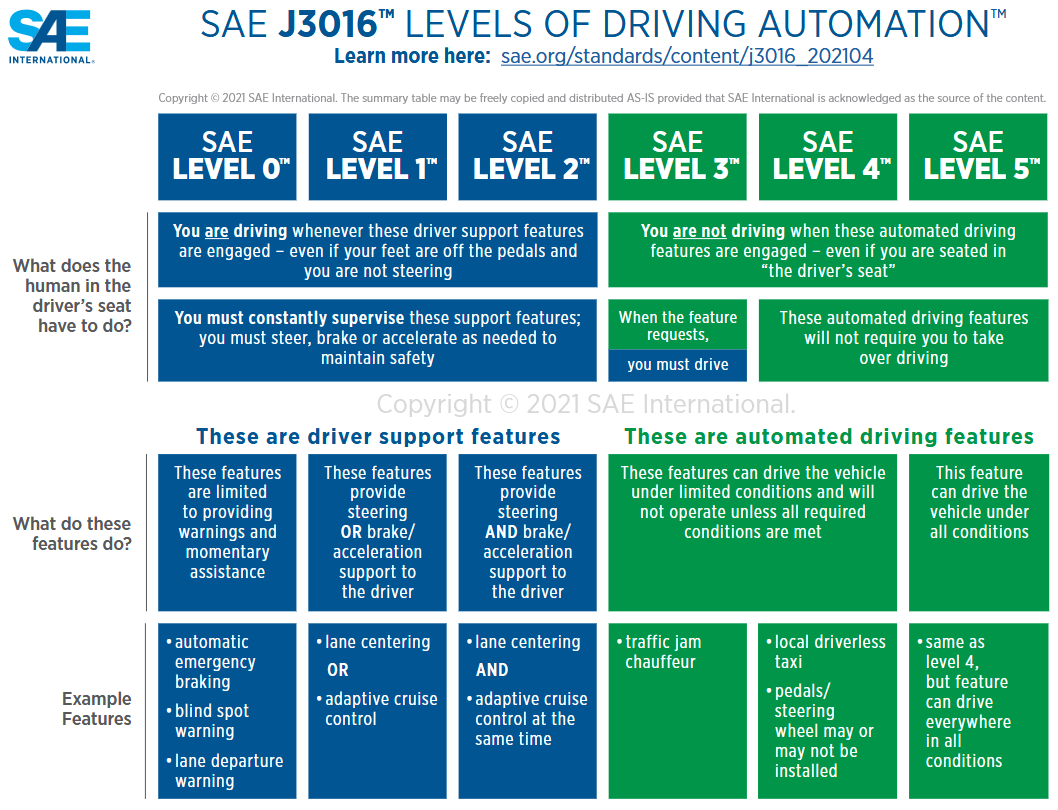
\includegraphics[width=0.99\textwidth]{fig_1_1_sae_automation_levels.png}
  \caption[SAE levels of driving automation.]{SAE levels of driving automation.}\label{fig:1.1}
\end{figure}

Each trend makes sense on its own, but together they cause a problem. The classical frameworks, led by ISO 26262:2018, were made for systems whose behaviour can be derived from a specification written beforehand, checked with tests that have expected outputs, and validated before deployment. Learned components break all three assumptions. Their behaviour comes out of a stochastic optimisation, there is no clear \enquote{correct answer} to compare their output with, and their robustness outside the training data can only be measured empirically. One of the first systematic studies of this problem is Salay, Queiroz and Czarnecki~\cite{salay2017}. They found five specific areas where ML affects ISO 26262, from new types of hazard to the fact that about 40\,\% of the Part 6 software techniques at unit level do not apply to ML components at all. That paper is the direct starting point of this work. Research and industry have responded with two partial strategies. One is containment, with monitor-actuator architectures or \emph{safety cages}\sidenote{A safety cage is a set of fixed, hand-written rules between the learned policy and the vehicle. It checks every command and replaces the ones that break a rule. The cage of this work has six rules (Chapter~\ref{ch:05}).}~\cite{kuutti2019,kuutti2021b}. The other is scenario-based validation~\cite{degelder2024}. How to combine both inside a development cycle with traceability is still an open question.

The standards are also still catching up. Since 2022, ISO 21448 (SOTIF) accepts that static validation is not enough when the operational domain cannot be fully specified. ISO/IEC TR 5469:2024 gives the first systematic guidance on AI in safety functions and classifies AI technology elements by how well they can be verified. UL 4600 makes the \emph{safety case} the main way to present evidence~\cite{koopman2023}. All three are high-level guides. They give principles, but they do not describe a concrete life cycle that someone can run on a real project. This thesis works in that gap.

\section{Problem statement}
\label{sec:1.2}

\textbf{General level.} The standard functional safety methods of the automotive industry, especially the V-Model used by ISO 26262, cannot be used as they are for systems that include components trained with reinforcement learning. If they are used without changes, one of two things happens. Either the RL component is forced into a specification it cannot meet, and the process stops being honest about what the system does. Or the component is left out of the process, and traceability is lost. Neither option is acceptable for a system with safety consequences.

\textbf{Specific level.} The literature proposes several separate fixes: safety cages to contain policies~\cite{kuutti2019,kuutti2021b}, predictive safety filters~\cite{tearle2021} and scenario-based evaluation~\cite{degelder2024}. Each one deals with part of the problem, but they are not combined into one life cycle with explicit traceability in both directions. Some work does look at the whole cycle, mainly Ullrich et al.~\cite{ullrich2025}, who extend the classical V-Model for AI systems, and earlier work on adapting ISO 26262 to ML~\cite{salay2017,vasudevan2021}. These proposals stay abstract. They do not provide an executable version or a complete, documented application case. This thesis builds an executable version of that kind of framework and tests it by applying it to a real case.

\textbf{Concrete level.} To evaluate such a framework, it has to be run on a case that is complex enough to show the typical problems (specifying learned behaviour, the sim-to-real gap, monitoring during operation) but small enough for one researcher to handle. The case chosen here is lane following on a 1:14 scale vehicle, trained in Gazebo with PPO through a gymnasium–\allowbreak{}Gazebo–\allowbreak{}ROS2 interface. In the main version, the \emph{policy} is end-to-end from the front camera\sidenote{End-to-end: one network goes from the raw image to the command, with no separate, hand-built perception step in between.}: a CNN learns perception and maps the image to an action. The deterministic cage does not use the network. It uses its own vision-based lane estimator. This puts perception inside the loop on purpose, because that is the harder case. A second version uses a privileged state vector and serves as a control arm\sidenote{As in a clinical trial, the control arm is the comparison group: same cage, same scenarios, but perfect state information, so the difference between the arms can be attributed to perception.}. It isolates the effect of the cage and shows how much perception costs.

The main research question is:

\begin{quote}
\textbf{Can the ISO 26262 V-Model be adapted with a small, traceable set of changes so that it can include components trained with reinforcement learning inside a development cycle with a safety case, while keeping the two-way link between specification and V\&V that makes the standard valuable?}
\end{quote}

A second question checks whether the framework works in practice:

\begin{quote}
\textbf{When the framework is applied to a lane-following case with a PPO policy and a rule-based cage, does it produce consistent and traceable evidence about how the system behaves, including an honest description of the sim-to-real gap?}
\end{quote}

\section{Hypotheses}
\label{sec:1.3}

\begin{itemize}
  \item \textbf{H1 (construct).} A small, countable set of changes to the classical V-Model (five in this work) is enough to cover the typical failure modes of RL/AI components without breaking the overall structure of the standard.
  \item \textbf{H2 (operability).} Each change can be turned into concrete artefacts (documents, tests, automatic checkers) that can be produced and maintained with an effort in line with the rest of the project, and not as a huge extra cost.
  \item \textbf{H3 (usefulness).} When the framework is applied to the case study, it produces traceable evidence that supports a well-founded verdict on the behaviour of the system, including the limits of that verdict.
\end{itemize}

The three hypotheses are evaluated at the end of the work (Chapter~\ref{ch:11}). H1 is checked by looking at the structure of the framework, H2 by the adoption cost recorded in the decision log during the project, and H3 by how many Safety Requirements received a verdict.

\section{Objectives}
\label{sec:1.4}

\subsection{General objective}
\label{sec:1.4.1}

To design, implement and evaluate a methodological framework, the \emph{adapted V-Model}, for developing autonomous driving systems that include components trained with reinforcement learning. The framework brings together safety cages, scenario-based validation, runtime monitoring and two-way traceability in a single cycle, and stays consistent with ISO 26262, ISO 21448, ISO/IEC TR 5469 and UL 4600.

\subsection{Specific objectives}
\label{sec:1.4.2}

\begin{itemize}
  \item \textbf{SO1.} To describe precisely which hidden assumptions of the classical V-Model stop working when a component trained with reinforcement learning is added to a safety module. \emph{(\S\ref{sec:3.3}.)}
  \item \textbf{SO2.} To propose and justify a limited set of changes that address those assumptions and stay consistent with the standards. \emph{(\S\ref{sec:3.4}.)}
  \item \textbf{SO3.} To turn each change into concrete artefacts (specifications, tests, checkers, metrics) and to define how they are produced. \emph{(\S\ref{sec:3.5}; chapters~\ref{ch:04}–\ref{ch:08} carry it out.)}
  \item \textbf{SO4.} To apply the framework to the case study, both in the main camera version and in the state-vector version used as a baseline, until the system works, can be evaluated and has complete traceability. \emph{(Chapters~\ref{ch:04}–\ref{ch:08}.)}
  \item \textbf{SO5.} To measure the gap between the training environment and the real operating environment, as required by adaptation A5. \emph{(Chapter~\ref{ch:09}.)}
  \item \textbf{SO6.} To give a well-founded verdict on whether the Safety Requirements are met, and to state clearly where that verdict stops being valid. \emph{(Chapter~\ref{ch:10}.)}
  \item \textbf{SO7.} To evaluate the framework itself: what it costs to adopt, what it covers, and under which criteria it is enough or not enough. \emph{(Chapter~\ref{ch:11}.)}
\end{itemize}

\section{Contributions}
\label{sec:1.5}

The main contribution is a method, not a technical result. The lane-following system is not an important contribution by itself, since better trained versions exist on more capable vehicles. What this thesis adds is the framework behind the system and the documented evidence of how it was applied.

The thesis claims five contributions, C1–C5. They are different from the five \emph{adaptations} A1–A5 that make up the framework and are defined in \S\ref{sec:3.4}. The adaptations are the content of the framework. The contributions are what this work adds to the state of the art. In this chapter and in all later chapters, A1–A5 always means the adaptations.

\begin{itemize}
  \item \textbf{C1 — A single methodological framework.} An adapted V-Model with five explicit changes (A1–A5): module design is split into \emph{Cage Specification} and \emph{Training Specification}; unit testing is split into \emph{Cage Unit Tests} and \emph{Policy Behavioral Evaluation}; a runtime monitoring level is added as continuous validation; two-way traceability becomes a hard requirement; and operational validation is redefined so that it includes an explicit description of the sim-to-real gap.
  \item \textbf{C2 — An executable version.} Each change comes with the artefacts that implement it, including reusable templates and automatic checkers. The most important one is the traceability checker, which turns traceability into a gate that a script can pass or fail.
  \item \textbf{C3 — A complete, reproducible case study.} The framework is applied to a system built from scratch, in two versions whose comparison shows the cost of camera perception. Artefacts, training and evaluation scripts are versioned, and the run data is published.
  \item \textbf{C4 — Measurement of the sim-to-real gap.}  Gazebo (reference campaign) $\rightarrow$ the physical platform. The second step ends as a bring-up and not as a results campaign. Chapters~\ref{ch:09} and \ref{ch:10} say this openly instead of hiding it.
  \item \textbf{C5 — Self-evaluation of the framework:} what it cost to adopt, where it worked as expected and where it showed its limits, so that others can improve it later.
\end{itemize}

\section{Scope and limitations}
\label{sec:1.6}

\subsection{Scope}
\label{sec:1.6.1}

The framework is applied to one system (lane following with PPO and a cage) on one platform (a 1:14 RC vehicle on a controlled track). There is no comparison with a similar system developed with the classical V-Model. The function is lane following on a closed track with controlled lighting and weather. Planning, interaction with other vehicles and driving on public roads are not covered. In terms of SAE levels, the system is a level 2 function. Levels 4–5 are out of scope.

\subsection{Known limitations}
\label{sec:1.6.2}

\begin{itemize}
  \item \textbf{Author bias.} The same person designs, builds and evaluates the framework, so there is a risk of confirmation bias. This is partly reduced by strict traceability that others can audit and by a dated decision log.
  \item \textbf{N = 1.} One case is not enough to draw general conclusions about the framework. The argument for generalisation is \emph{structural}: the adaptations target assumptions that fail in any system with a learned component. It is not a statistical argument.
  \item \textbf{Adoption cost without comparison.} The effort spent on the framework's artefacts is recorded, but there is no control group.
  \item \textbf{The adaptations are not a complete list.} The five chosen here are the ones the author considers most relevant for this case. Others could also be justified.
  \item \textbf{Scale platform.} The findings on the sim-to-real gap apply to a 1:14 vehicle on a controlled track.
  \item \textbf{The physical step ends as a bring-up.} The deployment chain runs on the real vehicle and gives calibration results and structural findings. However, no scenario has been scored on hardware and the cage has never changed an action there. For this reason the physical column of the verdict table is marked \emph{not executed} (\S\ref{sec:10.4}), and all driving figures in Chapter~\ref{ch:09} are preliminary. This is a limit of the evidence, not of the framework, and the text says so wherever it matters.
\end{itemize}

These limitations are discussed further in \S\ref{sec:3.9} and in Chapter~\ref{ch:11}.

\subsection{Intended simplifications of the case study}
\label{sec:1.6.3}

The case study also contains technical simplifications. They were not chosen for convenience. They are experimental controls: each one fixes one layer of the system so that the layer this thesis studies can be looked at on its own. The system can be seen as a stack:

\begin{quote}
\texttt{perception → state (ey, epsi, v, κ) → [ policy + cage ] → actuation → dynamics}
\end{quote}

The contribution is in the \texttt{[policy + cage]} block, and in both tracks the cage rules are written over the abstract state. There are three simplifications.

\textbf{Two observation tracks.} The main system is the camera track. The policy drives from the image, and the cage reads its own deterministic CV estimator, so perception is a central part of the work. Next to it, the state track gets \texttt{(ey, epsi, v)} by projecting the true pose onto the centre line\sidenote{\texttt{ey} is the lateral offset from the lane centre, \texttt{epsi} the heading error relative to the lane direction and \texttt{v} the speed. All symbols are listed at the start of the document.}. This fixes the perception layer, which makes it possible to isolate the effect of the cage and to measure the cost of perception as the difference between the two tracks. The cage does not care where the state comes from. The safety verdicts are always measured on the true pose, because leaving the lane is a physical fact and not an estimator error.

\textbf{Speed authority of the policy.} The work uses two contracts. For most of the project, the learned component only controls steering and the speed stays constant. This reduces the problem to lateral control and keeps the rule \enquote{the reward guides, the cage guarantees}. In the final reference campaign the action includes both steering and throttle, so the policy also controls speed. Chapter~\ref{ch:08} shows that this changes the role of the cage in a way that can be measured.

\textbf{Two track layouts, one platform.} The state track is validated on an oval (R = 0.8 m) and the camera track on the \texttt{complex\_b} circuit, which is winding and comes close to itself (perimeter 19.22 m). Both use the 1:14 vehicle. The argument for other layouts is structural, supported by the second layout, and not based on exhaustive evidence.

These limits do not weaken the main claim, which is that the cage adds measurable and traceable safety to a learned component. They make it \emph{clean}. Because the neighbouring layers are fixed, the effect of the cage can be attributed clearly, without being hidden by perception noise or by the transfer to hardware. Each limit is discussed again in its experimental context in \S\ref{sec:8.2} and \S\ref{sec:8.8}.

\section{Structure of the document}
\label{sec:1.7}

The thesis has twelve chapters in four blocks, shown in Figure~\ref{fig:1.2}. Block I — Framework contains this introduction, the state of the art (Chapter~\ref{ch:02}) and the methodology (Chapter~\ref{ch:03}), which is the main academic contribution. Block II — Specification covers the operational domain, the hazard analysis and the derivation of requirements (Chapter~\ref{ch:04}), and the architecture with the cage specification (Chapter~\ref{ch:05}). Block III — Implementation and evaluation covers implementation and verification (Chapter~\ref{ch:06}), the training specification and how it was carried out (Chapter~\ref{ch:07}), the experimental evaluation campaign (Chapter~\ref{ch:08}) and the measurement of the sim-to-real gap in steps of increasing realism (Chapter~\ref{ch:09}). Block IV — Closure presents operational validation and the full verdict table (Chapter~\ref{ch:10}), a discussion of the framework against its own criteria (Chapter~\ref{ch:11}), and the conclusions and future work (Chapter~\ref{ch:12}).

\begin{figure*}[htbp]
  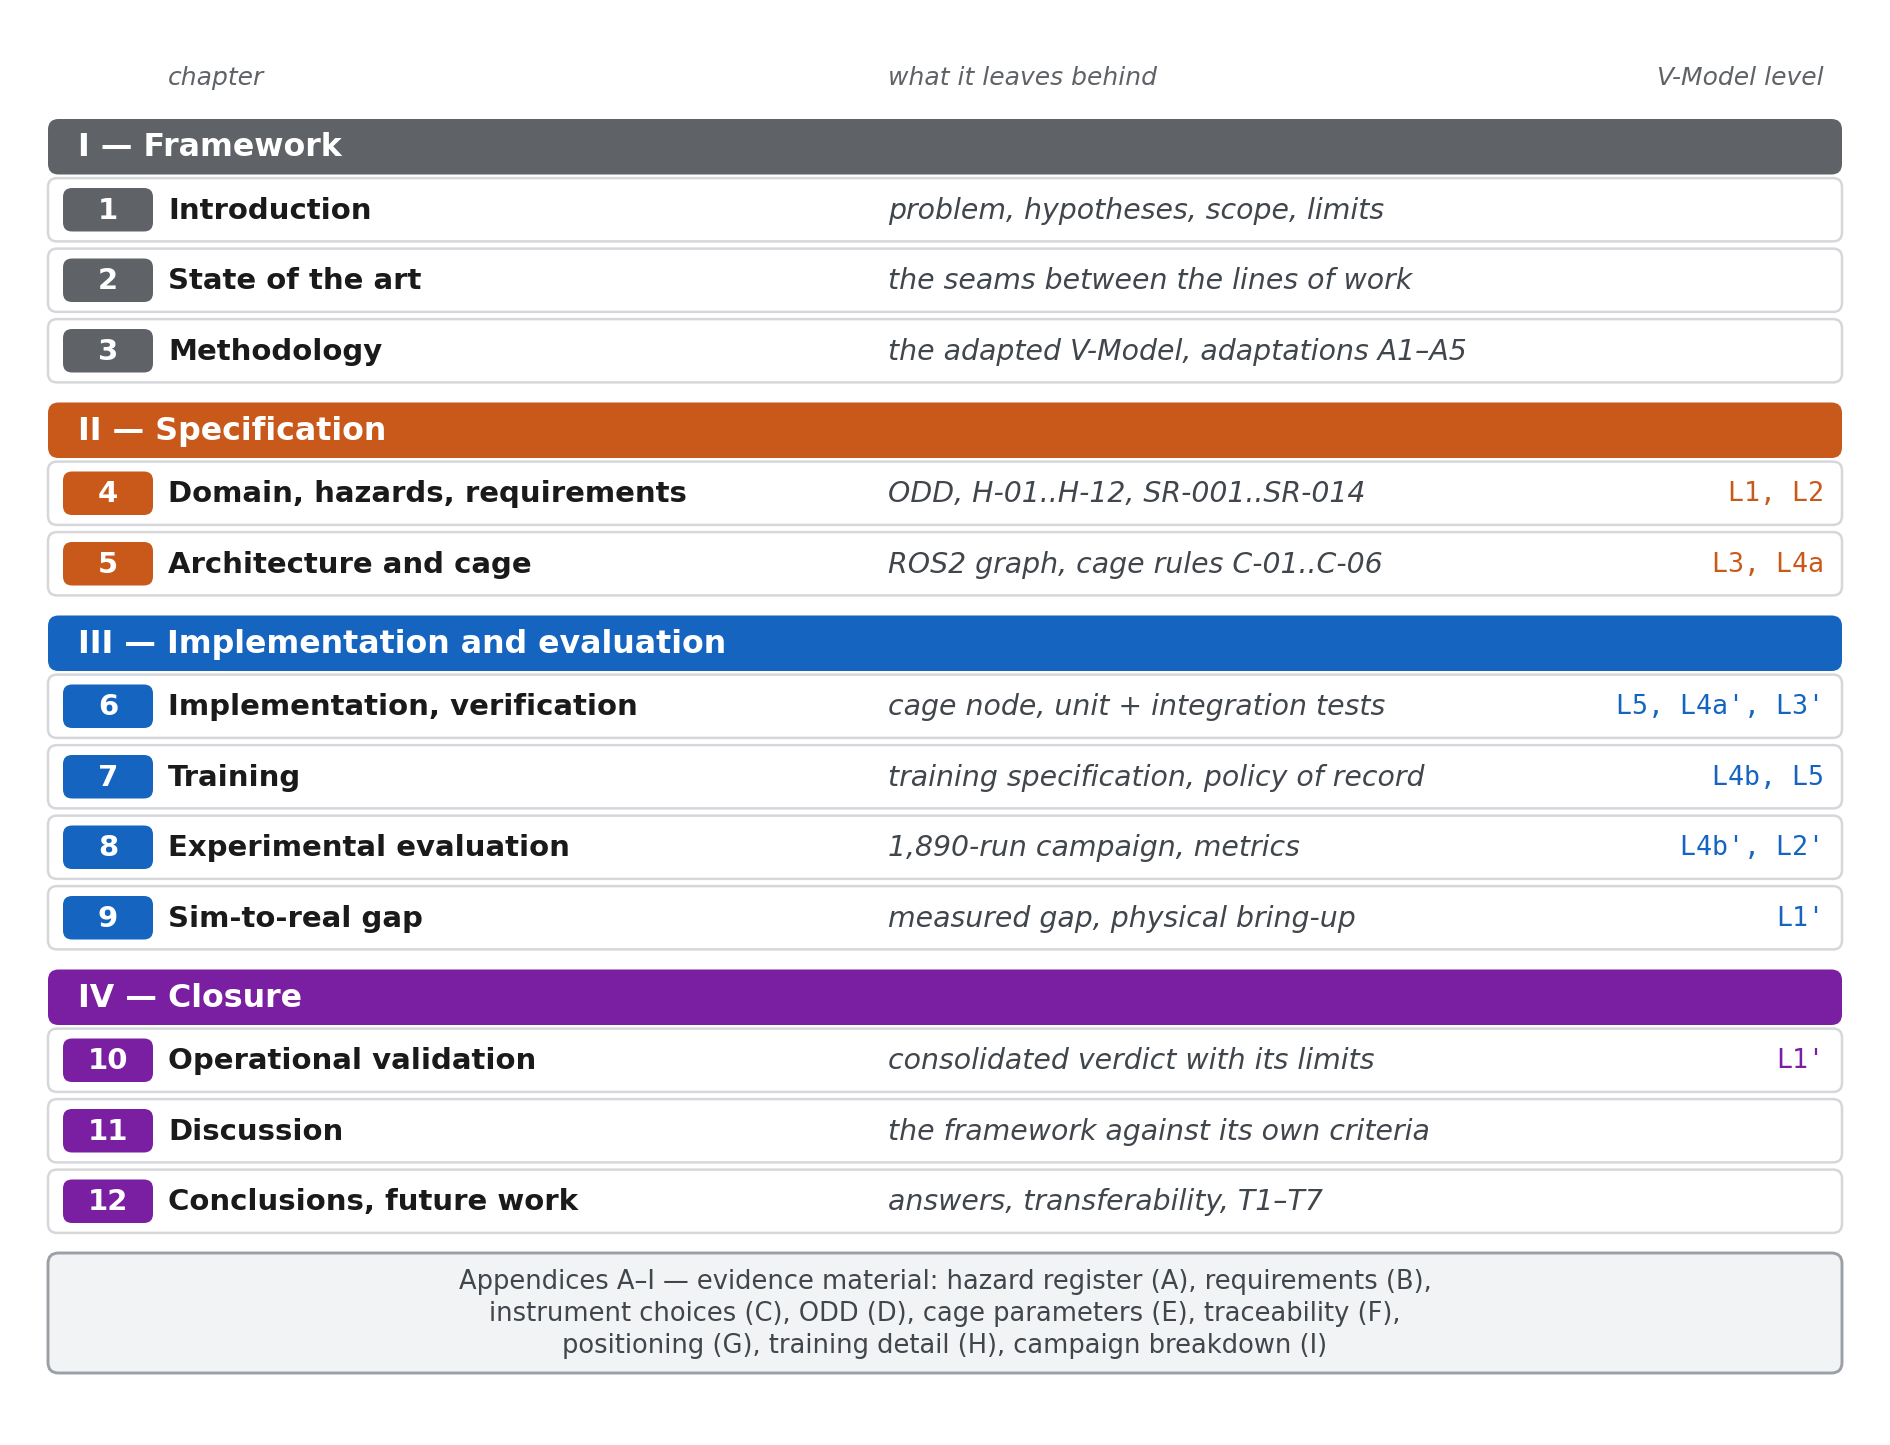
\includegraphics[width=1.00\widefigurewidth]{fig_1_2_document_roadmap.png}
  \caption[Reading map of the document.]{Reading map of the document: the four blocks, the twelve chapters, what each chapter produces, and which level of the adapted V-Model it belongs to. The formal mapping between levels and artefacts is not repeated here. It is given in Table~\ref{tab:3.3}, after the framework has been defined.}\label{fig:1.2}
\end{figure*}

The appendices contain the supporting material, so that the main text can stay readable: the extended hazard register (A), the requirements specification with its rationale (B), the choice of instruments and the mapping to the standards (C), the operational domain specification (D), the cage parameters (E), the traceability matrix (F), the full positioning space (G), the details of the training specification (H) and the scenario-by-scenario results of the reference campaign (I).

% GENERATED by md2tex.py from ../draft_v5_en/body/02_related_work.md -- do not edit by hand.
% Change the Markdown and run `python md2tex.py`; edits here are overwritten.

\chapter{State of the art}
\label{ch:02}

\section{Purpose and structure of the chapter}
\label{sec:2.1}

This chapter puts the relevant literature into a map and, most importantly, points out the places where lines of work do not connect, which is what this thesis tries to handle together. The review is selective: it focuses on work from the last seven years and on work that has clearly influenced the academic or standards discussion. It goes from general to specific: reinforcement learning in driving (\S\ref{sec:2.2}), groups of safety approaches (\S\ref{sec:2.3}), scenario-based validation (\S\ref{sec:2.4}), standards (\S\ref{sec:2.5}), life cycle adaptations (\S\ref{sec:2.6}) and the sim-to-real gap (\S\ref{sec:2.7}). It ends with a summary that places the thesis in this map (\S\ref{sec:2.8}).

\section{Reinforcement learning in autonomous driving}
\label{sec:2.2}

Machine learning for vehicle control has developed in three waves. The first was behaviour cloning, or \emph{imitation learning}. It showed that a network could map pixels to steering commands, but it broke easily when the vehicle moved away from the states the expert had shown. The second was deep reinforcement learning (DRL), which aimed to fix that problem by letting the agent explore the results of its own decisions~\cite{kuutti2021a}. The third wave is still ongoing. It mixes both approaches and adds world models and explicit safety representations.

\begin{figure}[htbp]
  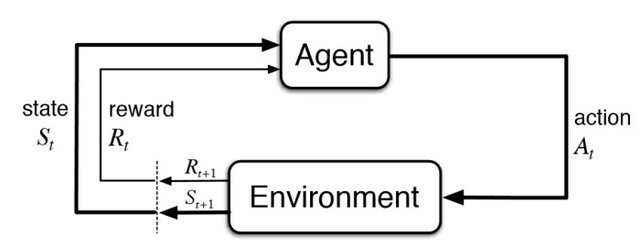
\includegraphics[width=0.99\textwidth]{fig_2_1_classical_rl_framework.png}
  \caption[The classical reinforcement learning framework.]{The classical reinforcement learning framework~\cite{sutton2018}. The agent chooses an action \texttt{At} in state \texttt{St} and receives the reward for it. Its goal is to maximise the total reward over a long sequence of transitions.}\label{fig:2.1}
\end{figure}

Two algorithms appear in most recent work. PPO~\cite{schulman2017} trains in a stable way thanks to its clipped loss\sidenote{PPO limits how far the policy can move in one update by clipping its objective. This keeps training stable, at the cost of needing more samples.}. This is useful when reproducibility matters and when sensitivity to hyperparameters causes practical problems. SAC~\cite{haarnoja2018} optimises a maximum-entropy objective that encourages exploration and robustness, and because it is \emph{off-policy}\sidenote{An off-policy method can learn from experience collected by older versions of the policy, kept in a replay buffer. An on-policy method such as PPO only uses fresh experience.} it needs fewer samples. This work uses both, and Chapter~\ref{ch:07} compares them in experiments.

For lane following specifically, Cheng et al.~\cite{cheng2025} show on a small physical platform (Duckiebot) that camera-based DRL policies trained in simulation can keep the lane on a real track. For the harder navigation task, however, domain randomization alone does not transfer, and what makes it work is image style transfer with CycleGAN. Zhao et al.~\cite{zhao2024} look at decision making on highways with constrained CMDP-type policies and a \emph{replay buffer}. The trend is clear. For short decision horizons and limited domains, DRL gives good results. For long horizons and open domains, the community agrees that DRL alone is not enough without extra guarantees.

End-to-end driving from vision has its own history, and the main track of this thesis builds on it. ALVINN~\cite{pomerleau1989} used a very small network on 30$\times$32 pixels. \mbox{DAVE-2}~\cite{bojarski2016}, later called PilotNet, scaled the idea to real roads with behaviour cloning. Kendall et al.~\cite{kendall2019} then used DRL to train lane following from a single camera image on a real vehicle. At the same time, domain randomization\sidenote{Domain randomization trains on many randomly varied copies of the simulated world (lighting, textures, dynamics), so that the real world looks like one more variation.}, both visual~\cite{tobin2017} and dynamic~\cite{peng2018}, became the usual way to make learned perception less fragile. The argument against end-to-end learning is just as old and is about sample complexity. Shalev-Shwartz and Shashua~\cite{shalevshwartz2016} show that splitting the problem through a semantic abstraction needs far fewer examples than a network that must learn the same function end to end. This supports keeping any component that needs a safety argument, here the envelope, outside the network. This thesis follows that line, but its contribution is not the end-to-end driver. It is the safety tooling around it. The runtime envelope does not use the learned network. It works on a classical, deterministic lane estimator that uses a different algorithm. Visual degradation also becomes something that scenarios control and evaluate, and not only noise added during training.

All of this work shares the same basic problem: the behaviour of the policy cannot be derived from a specification written beforehand. That breaks the main assumption of the classical functional safety frameworks.

\section{Safety approaches for systems with learned components}
\label{sec:2.3}

The literature can be grouped into four families. Each one looks at the problem from a different point in the life cycle.

\textbf{(a) Safe RL: safety inside training.} The classical taxonomy comes from García and Fernández~\cite{garcia2015}. It has two axes: changing the optimisation criterion and changing the exploration process. Recent work adds explicit safety information to the state space or the value function. The SRPL framework~\cite{mani2025} adds to the state a learned model that predicts future constraint violations. Keswani and Bhattacharyya~\cite{keswani2025} test it on real driving datasets and report statistically significant gains in success rate and cost compared with the same safe RL optimisers without it. They also say that these gains depend on the optimiser and on the dataset. The idea is elegant, but it has the same basic limit as the whole family: the guarantee is statistical, it depends on the training distribution, and it does not carry over automatically to a different operational domain.

\textbf{(b) Safety cages and runtime filters.} This family complements the first one. It works at inference time and treats the policy as a black box whose outputs need to be filtered. Kuutti et al.~\cite{kuutti2019} take the \emph{safety cage}, an idea already proposed for autonomous vehicles in earlier work, and apply it to a controller based on a deep network. The cage is a deterministic module that watches the network's outputs and replaces them with a safer action when the proposed behaviour would go past its limits. Since its rules are easy to interpret, classical functional safety validation methods can be used on it. The same paper already uses the interventions to retrain the network. Kuutti et al.~\cite{kuutti2021b} then put the cages inside reinforcement learning training, where they play two roles: containment and weak supervision of the agent. In that setup the cage does not only contain the agent but also \emph{shapes} how it behaves. This double role shows up again, without being planned, in the findings of Chapter~\ref{ch:08}.

\begin{figure}[htbp]
  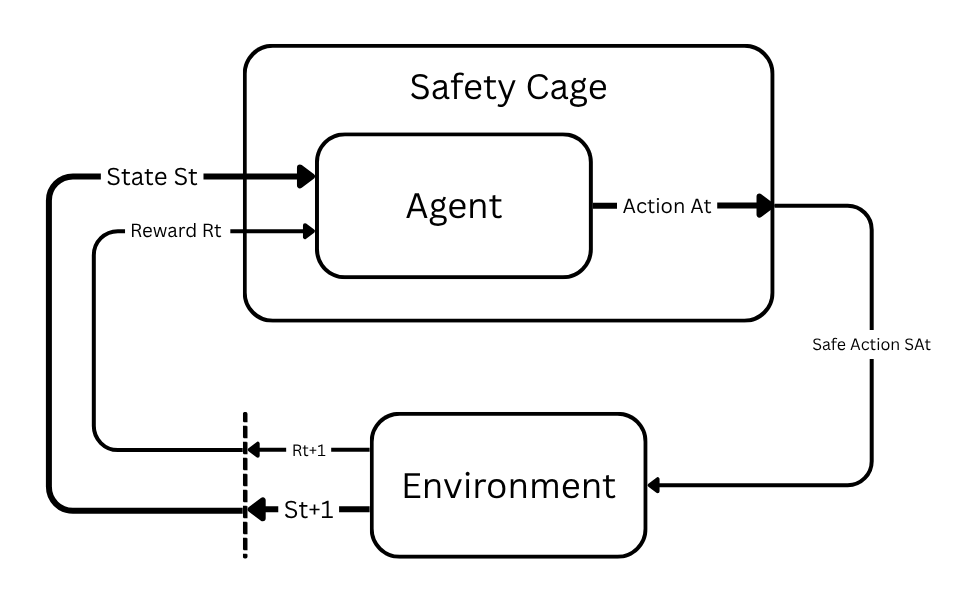
\includegraphics[width=0.99\textwidth]{fig_2_2_safety_cage_idea.png}
  \caption[The safety cage applied to the classical RL framework.]{The safety cage applied to the classical reinforcement learning framework.}\label{fig:2.2}
\end{figure}

A related line proposes \emph{predictive safety filters} based on model predictive control. Instead of checking each action on its own, the filter predicts what the proposed action will lead to. If a safe backup trajectory into the safe set still exists, the action is applied. If not, it is replaced by the closest input that keeps such a trajectory~\cite{tearle2021}. The strength of this approach is its formal clarity. Its practical weakness is that it needs a fairly accurate dynamic model, which is hard to get with noisy perception. The architecture goes back to the Simplex pattern\sidenote{In the Simplex pattern a simple, verified controller watches a complex one and takes over when the system gets close to an unsafe state.}~\cite{sha2001}, where a complex controller is supervised by a simple, verified one, and to the related formal method of \emph{shielding}~\cite{alshiekh2018}. A shield intervenes as little as possible: it only overrides an action when that action would break the safety specification. The cage in this thesis is a Simplex instance with deterministic rules. It sits between the cage of Kuutti et al., from which it takes verifiable containment, and the formal \emph{shield}, whose idea of minimal intervention it copies in its rate-limiting rule.

\textbf{(c) Robustness against perturbations.} He et al.~\cite{he2024} test a Q-learning controller on TORCS against two threat models, with a result that matters for method: perturbations on the sensors have almost no effect (attack success rate close to zero, because the action space is discrete), while directly changing the action works between 60\,\% and 78\,\% of the time. Discretisation gives \emph{accidental} robustness on one channel and leaves the other one open. Wei et al.~\cite{wei2026} attack the same problem from the defence side: they focus observation perturbations on a few safety-critical moments with a limited budget and train with a dual \emph{replay buffer} of normal and adversarial experience. The lesson is direct: testing a policy must include how it reacts to inputs and outputs outside the normal distribution, and the cage must be designed on the assumption that both the policy and its interfaces can fail.

\textbf{(d) Runtime monitoring.} This family cuts across the other three and is about detecting errors while the system is running. Mohseni et al.~\cite{mohseni2019} organise the field around five gaps that ML opens in the classical standards: specification, transparency, verification, performance and \emph{runtime monitoring}. They link the techniques for each gap to classical safety engineering strategies such as safe fail and safety margins. What matters most for this thesis is that they treat monitoring as its own architectural category, with three groups of techniques: uncertainty estimation, in-distribution error detection and out-of-distribution detection. Adaptation A3 in Chapter~\ref{ch:03} takes this idea directly. Vasudevan et al.~\cite{vasudevan2021} continue the line and propose evidential deep learning~\cite{sensoy2018} to quantify uncertainty in a way that explicitly follows ISO 26262.

The four families complement each other. They are not alternatives, and a mature system should use parts of all of them. The literature, however, usually presents them as separate contributions, with no framework that brings them together inside a life cycle with traceability and a safety case. This is one of the gaps this thesis identifies.

\section{Scenario-based validation}
\label{sec:2.4}

The previous section is about how to \emph{build} safe systems. This line is about how to \emph{evaluate} them. The main question is what it means to validate a system whose operational domain is continuous and, strictly speaking, infinite. The most common answer is to test against a curated library of representative situations instead of trying to cover everything.

The theoretical problem behind this is coverage.\sidenote{Coverage: how much of the operational domain the scenario library actually exercises. Without a measure of it, no library size can be called enough.} De Gelder et al.~\cite{degelder2024} propose metrics for what it means for a scenario database to \emph{cover} the domain: whether it captures all relevant aspects of the ODD, described with tags, and whether it covers the driving data it came from in time and in actors involved. They also argue that simply counting concrete parameterised scenarios cannot give a meaningful coverage number. Without such metrics, any library can be called \enquote{sufficient} with circular arguments. In practice, CARLA~\cite{dosovitskiy2017} has become the reference urban simulator: Gao et al.~\cite{gao2021} build on it a combined metric calibrated against human raters, and Paniego et al.~\cite{paniego2024} publish an open tool that organises how metrics are collected and aggregated in simulation, for both CARLA and Gazebo.

A newer line uses reinforcement learning to generate test scenarios. Giamattei et al.~\cite{giamattei2025} replicate and extend earlier work and find something unexpected: once the biases in collision measurement are removed, RL does no better than random sampling. Only after fixing the reward function and adapting the algorithm to the continuous space does its theoretical advantage turn into a real improvement. The practical lesson is that the quality of the failure metric matters more than how advanced the method looks. This lesson applies directly to the design of the campaign in Chapter~\ref{ch:08}.

The shared limitation of this line is that it covers evaluation but not the life cycle. It is a necessary part of a methodological framework, but it is not a framework by itself.

\section{Standards and normative frameworks}
\label{sec:2.5}

Five documents shape the standards landscape, and none of them covers it completely.

\textbf{ISO 26262:2018}~\cite{iso26262} sets up the functional safety framework and makes the V-Model the reference life cycle. Its known limitation is that it assumes deterministic systems that can be specified in advance. ISO 21448:2022 (SOTIF)~\cite{iso21448} widens the scope to hazardous behaviour that does not come from faults but from limits of the function under conditions nobody anticipated. It is the first official response to the fact that a system with ML can behave wrongly without anything having \enquote{failed} in the classical sense. Wang et al.~\cite{wang2024}, in a view that is important for this thesis, review SOTIF across development, verification and validation, and operation, and describe the algorithm-level work as a V-Model extended with an operation phase centred on runtime monitoring. ISO/IEC TR 5469:2024~\cite{isotr5469} is the most specific document on AI in safety functions. It classifies AI technology along two axes. One is how the AI is used in the system. The other is a technology class: Class I means the technology can be developed and reviewed with existing functional safety standards. Class II means extra methods are also needed to reach the required properties. Class III means no known methods are enough. The TR puts deep learning models most likely in Class II or III. It also proposes a three-stage realisation principle. ISO/PAS 8800:2024~\cite{isopas8800} is the automotive document on AI and is closely linked to TR 5469. It extends ISO 26262 and ISO 21448 to AI elements by adapting the relevant ISO 26262 clauses and extending the SOTIF concepts. An example use case published by BSI for the UK CCAV~\cite{hawkins2025}, on an ML traffic-sign detector, shows how ISO 26262, SOTIF and PAS 8800 can be combined for an ML component. UL 4600~\cite{ul4600} formalises the \emph{safety case}\sidenote{A safety case is a structured argument, backed by evidence, that a system is acceptably safe for a given use in a given environment.} with a claim–\allowbreak{}argument–\allowbreak{}evidence structure~\cite{koopman2023}.

\begin{figure*}[htbp]
  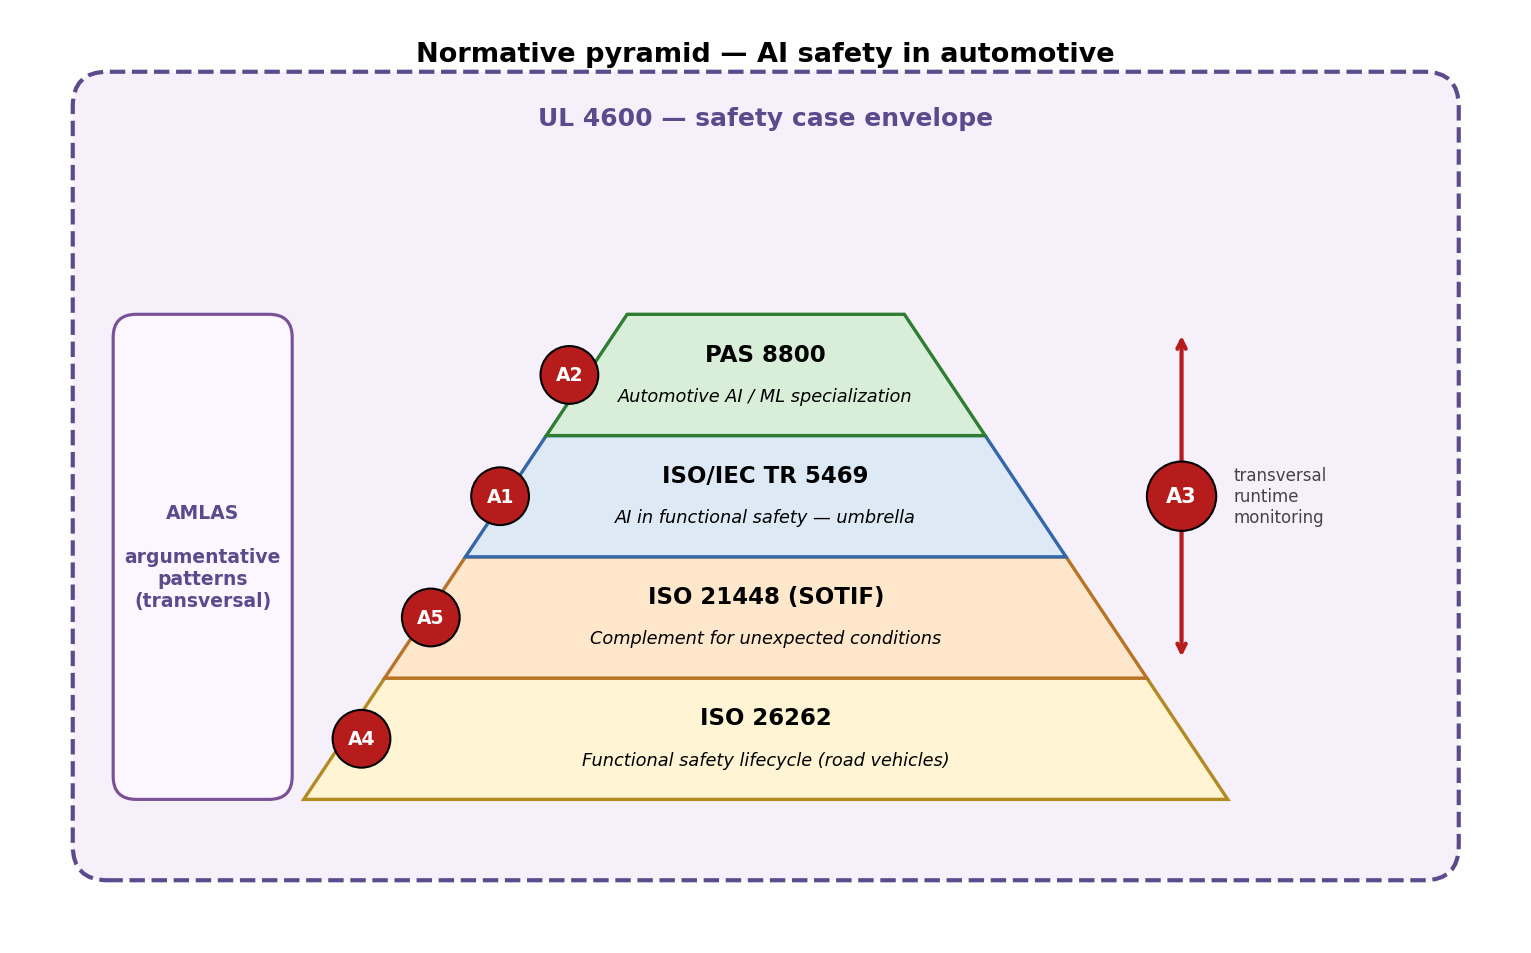
\includegraphics[width=0.71\widefigurewidth]{fig_3_6_normative_pyramid.png}
  \caption[Applicable normative pyramid.]{Normative pyramid: ISO 26262 as the base life cycle, SOTIF as the complement for unexpected conditions, TR 5469 as the general AI layer, PAS 8800 as the automotive AI extension, UL 4600 as the safety case around everything, and AMLAS as argument patterns that apply across all of them.}\label{fig:2.3}
\end{figure*}

Outside the standards, two reviews complete the picture. Wäschle et al.~\cite{waschle2022} carry out a systematic review of AI safety in highly automated driving, keeping 102 publications after screening. They separate established approaches from new ML-specific ones and point out that claims about the performance of learned components are always statistical, and that safety standards still need to be extended to AI. Paterson et al.~\cite{paterson2025} consolidate AMLAS, a six-stage method with GSN patterns\sidenote{GSN, Goal Structuring Notation: a graphical way to draw a safety argument as goals, the strategies that break them down, and the evidence that supports them.} for building safety arguments about ML components, aligned with a data-centred life cycle. AMLAS provides the argumentation part that was missing, and it is now being included in the new standards.

In short, each document covers something necessary: the classical cycle, unexpected conditions, the nature of AI, its automotive extension, how to structure evidence, and argument patterns. None of them gives an executable method that combines them in a real project. That work is left to the engineering team, and it is exactly what this thesis proposes.

\section{V-Model adaptations for systems with AI}
\label{sec:2.6}

The work closest to this thesis is the work that explicitly adapts the life cycle.

Salay, Queiroz and Czarnecki~\cite{salay2017} are the starting point. They go through the ten parts of ISO 26262 and find five areas of impact: hazard identification (including RL-specific failure modes such as \emph{reward hacking}), faults and failure modes, using training sets instead of specifications, the architectural level compared with the implementation unit, and whether the Part 6 techniques still apply. Of the Part 6 software techniques that apply at unit level, which are 34 of the 75, they find that about 40\,\% do not apply to ML components at all. The main reason is that these techniques were written for imperative programming languages. Assumptions S1–S5 in Chapter~\ref{ch:03} restate that analysis in operational form.

Ullrich et al.~\cite{ullrich2025} are the most relevant current reference. They propose concrete structural changes to the classical V-Model: iterative loops between levels, explicit data-centred phases, runtime monitoring as an extended right arm, and artefacts specific to data-driven development. They also already include explicit stages for moving the system from simulation to real data and for evaluating that move. The difference with this thesis is in the kind of work, not in the goal. Ullrich et al. describe \emph{what} to do, as a framework that can be reused, and only sketch how to apply it. This thesis works on \emph{how} to do it, in three areas they leave open: an executable version of each change, a complete documented case, and an empirical measurement of the sim-to-real gap on a real platform.

Vasudevan et al.~\cite{vasudevan2021} are an intermediate step. Their work is limited to handling uncertainty and has no complete application case. Sprockhoff et al.~\cite{sprockhoff2023}, from aerospace, add a different view based on model-based systems engineering. Their idea is that the model, not the text documentation, is the central artefact. This fits well with the strict traceability that AI systems need. However, industrial MBSE tools take a long time to learn, which makes them hard to use in smaller projects. There, version-controlled text files are more practical and give the same function.

Apart from these works, there is very little literature on life cycle adaptations compared with the literature on individual aspects. This makes sense, since individual contributions are easier to publish and easier to evaluate cleanly. But it explains why the industrial use of AI in safety functions is still \emph{ad hoc} and depends on the judgement of each team instead of a shared framework.

\section{The sim-to-real gap and its measurement}
\label{sec:2.7}

Every policy trained in simulation faces the same question when it is deployed: how much of the learned behaviour carries over? The techniques to reduce the gap fall into three groups that work together. Domain randomization trains on many different simulated variants. Domain adaptation adjusts the policy or its representations to the real domain with a small amount of data. System identification improves the simulation by calibrating it with physical data.

But the problem is not only reducing the gap. It is also describing it honestly. A deployed system can work well on average and fail badly under specific conditions that nobody measured. The literature has many proposals for reducing the gap and very few systematic frameworks for \emph{measuring} it in a form that is useful for a safety case. This is why adaptation A5 makes measuring the gap a required level of the life cycle.

The simulator used here is Gazebo~\cite{koenig2004}, and the choice is justified in \S\ref{sec:3.6}. What matters for this section is only its consequence: its visual quality is lower than that of the engines behind CARLA, so the gap that A5 asks to measure is expected to be larger. Whatever the simulator, for 1:14 scale vehicles the match between simulated and real dynamics has its own differences — tyre friction, loop delays, noise from the onboard sensors — that need to be measured. Cheng et al.~\cite{cheng2025} are the closest precedent, but like the rest of the literature they focus on \emph{reducing} the gap and not on measuring it systematically. That measurement is the topic of Chapter~\ref{ch:09}.

\section{Critical summary and positioning}
\label{sec:2.8}

The table below summarises the state of the art along seven axes. The full version, with the twenty lines of work reviewed, is in Appendix~\ref{app:G}.

% layout: table*, fixed, \small, 164 of 165 mm
\begin{table*}[htbp]
\caption{Positioning of the thesis (short version; full version in Appendix~\ref{app:G}).}\label{tab:2.1}
\small\setlength{\tabcolsep}{4pt}
\begin{tabular}{@{}>{\RaggedRight\arraybackslash}p{75.7mm}>{\centering\arraybackslash}p{10.5mm}>{\centering\arraybackslash}p{10.5mm}>{\centering\arraybackslash}p{10.5mm}>{\centering\arraybackslash}p{5.1mm}>{\centering\arraybackslash}p{10.5mm}>{\centering\arraybackslash}p{10.5mm}>{\centering\arraybackslash}p{10.5mm}@{}}
  \toprule
  \tabhead{Line of work} & \rotatebox{90}{\tabhead{Safe training}} & \rotatebox{90}{\tabhead{Cage / filter}} & \rotatebox{90}{\tabhead{Scenarios}} & \rotatebox{90}{\tabhead{Life cycle}} & \rotatebox{90}{\tabhead{Explicit traceab.}} & \rotatebox{90}{\tabhead{Sim-to-real gap}} & \rotatebox{90}{\tabhead{E2E case}} \\
  \midrule
  Safe RL (García and Fernández; Keswani; Wei) & \ding{51} & – & – & – & – & – & – \\
  \addlinespace[2pt]
  Safety cages and filters (Kuutti; Tearle) & partial & \ding{51} & – & – & – & – & – \\
  \addlinespace[2pt]
  Scenario-based validation (De Gelder; Gao; Paniego) & – & – & \ding{51} & – & – & – & – \\
  \addlinespace[2pt]
  Applied sim-to-real (Cheng et al.) & partial & – & – & – & – & partial & partial \\
  \addlinespace[2pt]
  Standards and safety case (SOTIF; UL 4600; AMLAS; PAS 8800) & – & – & partial & \ding{51} & partial & – & partial \\
  \addlinespace[2pt]
  Life cycle adaptation (Salay; Ullrich; Sprockhoff) & partial & partial & partial & \ding{51} & partial & partial & – \\
  \addlinespace[2pt]
  \textbf{This thesis} & \textbf{partial} & \textbf{\ding{51}} & \textbf{\ding{51}} & \textbf{\ding{51}} & \textbf{\ding{51}} & \textbf{\ding{51}} & \textbf{partial} \\
  \bottomrule
\end{tabular}
\end{table*}

Three points come out of the table.

\textbf{First.} The individual contributions are solid and often go deep. It is not reasonable, or necessary, to try to beat them on any single axis. The thesis uses existing solutions for training (PPO), for containment (the safety cage tradition) and for validation (scenario-based methods).

\textbf{Second.} Some proposals do adapt the life cycle, and several of the changes in this thesis already appear there in some form. Runtime monitoring as an extended right arm comes before A3, and the GSN patterns of AMLAS share the same idea as the two-way traceability of A4. So the new part is not the adaptations themselves. It is three things that no earlier work covers together. The first is an executable version: each adaptation is turned into artefacts and checkers instead of staying a recommendation. The second is traceability as a hard constraint: it becomes a property that a tool checks, which goes further than the descriptive level of AMLAS and of model-based engineering. The third is a complete application case, with the problems and real costs documented.

\textbf{Third.} Measuring the sim-to-real gap is the least covered axis, for the imbalance described in \S\ref{sec:2.7}. Adaptation A5 and Chapter~\ref{ch:09} are a specific contribution on that axis, with external validity limited to a scale vehicle on a controlled track.

With this overview in place, Chapter~\ref{ch:03} presents the methodological framework, which is the main academic contribution of the thesis.

% GENERATED by md2tex.py from ../draft_v5_en/body/03_methodology.md -- do not edit by hand.
% Change the Markdown and run `python md2tex.py`; edits here are overwritten.

\chapter{Methodology}
\label{ch:03}

\section{Purpose of the chapter}
\label{sec:3.1}

This chapter presents the main methodological contribution of the thesis: the adapted V-Model. It is a life cycle framework for systems that include components trained with reinforcement learning inside functions that affect safety. The chapter defines the framework used in the rest of the work, explains the decisions behind it, and relates each decision to the standards and to the literature from Chapter~\ref{ch:02}. It does not present experimental results or implementation details.

Two things are often mixed up and should be kept apart. The \emph{research methodology}, meaning how this work produces knowledge that can be generalised, is covered in \S\ref{sec:3.2}. The \emph{system engineering methodology}, meaning how the technical system is built from requirements to deployment, is covered in \S\ref{sec:3.3} to \S\ref{sec:3.8}. The first answers the question \enquote{what does this thesis add to knowledge?}. The second answers \enquote{how is the system built?}. Chapters~\ref{ch:04} to \ref{ch:10} put into practice what is defined here, and Chapter~\ref{ch:11} evaluates the framework based on that practice.

\section{Research approach}
\label{sec:3.2}

\subsection{Type of research}
\label{sec:3.2.1}

The work follows the \emph{design science research} tradition\sidenote{In design science the contribution is a useful artefact, here the adapted V-Model. It is judged by how well it solves the problem when it is used, not by a statistical test.}~\cite{march1995,hevner2004}. In this tradition, the academic contribution is not an empirical claim tested against reality, and not a logical statement proved by deduction. It is an artefact that solves a known problem, and its usefulness is evaluated through one or more application cases.

The artefact here is the adapted V-Model, which consists of five adaptations A1–A5 to the ISO 26262 V-Model, together with the templates, checkers and other artefacts that implement it. This has three consequences. First, the thesis does not aim for the usual result of an empirical thesis, such as finding a phenomenon or rejecting a statistical hypothesis. It aims to build a useful artefact and show that it works. Second, the evaluation looks at the artefact and not only at the system built with it, so one chapter is dedicated to evaluating the framework itself (Chapter~\ref{ch:11}). Third, generalisation is argued through structure, because the adaptations target V-Model assumptions that fail for any system with a learned component, and not through statistics over many cases.

\subsection{Evaluation strategy: one case study}
\label{sec:3.2.2}

The framework is evaluated on a single case: lane following on a 1:14 scale vehicle, trained with PPO in Gazebo and supervised by a deterministic safety cage. The reason is feasibility. A case that covers the whole cycle, from HARA to deployment, is already a lot of work for a master's thesis. Doing several would make each one shallow, which does not fit the rigour that the framework itself asks for. One deep case is better than several shallow ones. The price is lower external validity. This is reduced in two ways: the structural argument, and a clear statement in Chapter~\ref{ch:12} of which parts of the framework can be reused and which parts need to be rethought.

\subsection{Role of the author}
\label{sec:3.2.3}

The author designs the framework, builds the system and evaluates the result. Doing all three creates a built-in risk of confirmation bias, and this has to be admitted before trying to reduce it. It is handled on three levels. The first is two-way traceability as a hard constraint (A4). An automatic checker enforces it and reports any orphan without the author being involved, so it works as a cheap external auditor. The second is the dated decision log. It records what was decided, which alternatives were rejected and why, and others can audit it later. The third is a clear list of limitations (\S\ref{sec:3.9} and Chapter~\ref{ch:11}), written as critically as if the solution were someone else's. None of these removes the bias, and nothing could. What they do is limit it to what an independent person could check in the version-controlled artefacts.

\section{The classical V-Model and its hidden assumptions}
\label{sec:3.3}

The V-Model comes from systems engineering~\cite{forsberg1991} and is the reference process model in ISO 26262. It organises development into five levels, with a two-way link between specification (left branch, going down) and verification and validation (right branch, going up).

\begin{figure*}[htbp]
  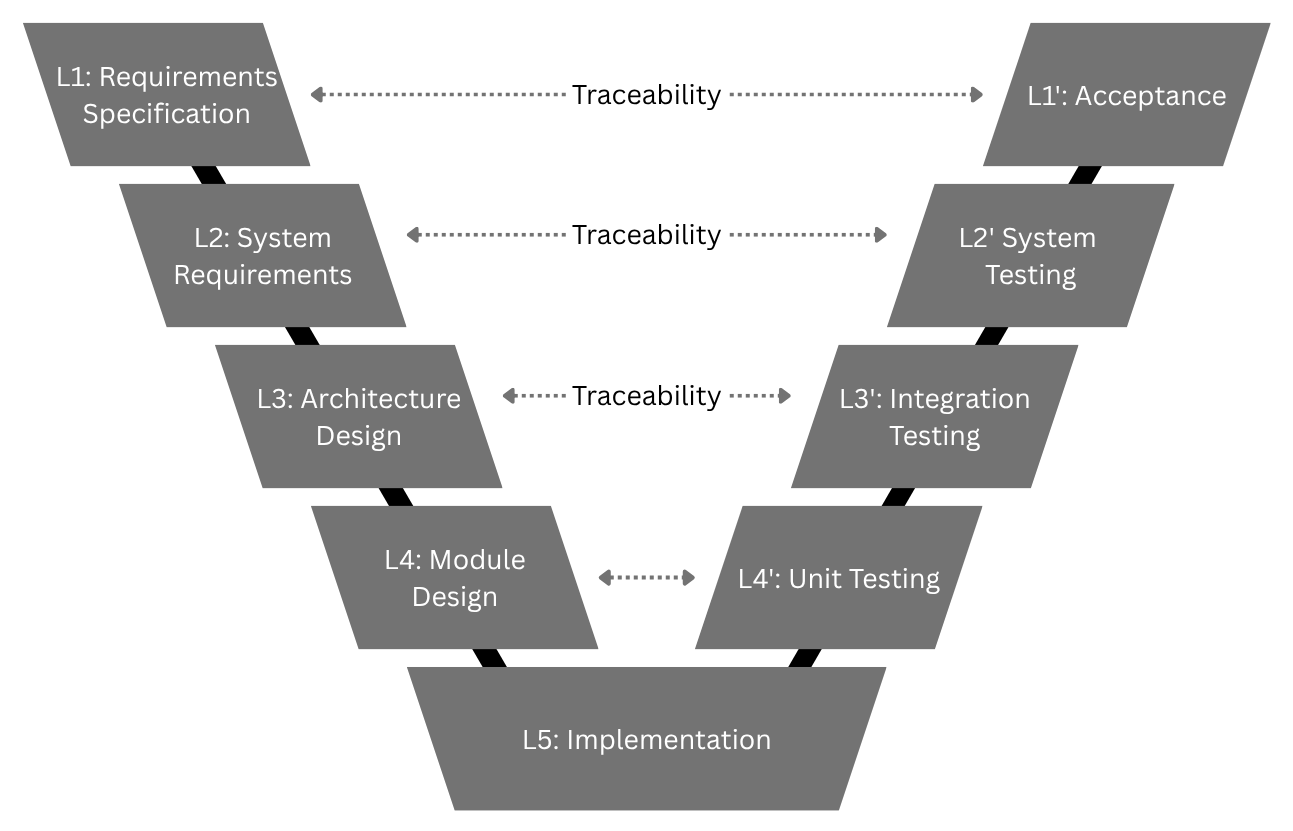
\includegraphics[width=0.77\widefigurewidth]{fig_3_1_adopted_classical_v_model.png}
  \caption[V-Model adopted by ISO 26262, instantiated on the lane-following case.]{V-Model adopted by ISO 26262 (simplified), applied to the lane-following case.}\label{fig:3.1}
\end{figure*}

The model relies on five assumptions. They are rarely written down, but the whole structure depends on them. Salay, Queiroz and Czarnecki~\cite{salay2017} were the first to identify them systematically. The assumptions S1–S5 below are a practical rewrite of their analysis, set up so that each one has a matching adaptation in \S\ref{sec:3.4}.

% layout: table*, fixed, \small, 164 of 165 mm
\begin{table*}[htbp]
\caption{The five assumptions of the classical V-Model and how they fail for learned components.}\label{tab:3.1}
\small\setlength{\tabcolsep}{4pt}
\begin{tabular}{@{}>{\RaggedRight\arraybackslash}p{19.5mm}>{\RaggedRight\arraybackslash}p{55.7mm}>{\RaggedRight\arraybackslash}p{82.8mm}@{}}
  \toprule
  \tabhead{Assumption} & \tabhead{Statement} & \tabhead{Why it fails for an RL component} \\
  \midrule
  S1 & Every module has a complete and deterministic specification written in advance & The policy has no designed specification: it comes out of training. No document says \enquote{when the input is Y, produce Z} \\
  \addlinespace[2pt]
  S2 & The behaviour can be derived reliably from the specification & The behaviour can be observed \emph{post hoc} but cannot be predicted analytically \\
  \addlinespace[2pt]
  S3 & Unit tests check compliance with finite coverage & There is no \enquote{correct} output for each input, only statistically plausible outputs \\
  \addlinespace[2pt]
  S4 & Static verification is enough to guarantee the properties & The policy can pass the tests and still fail in operation, because of state distributions that were not tested \\
  \addlinespace[2pt]
  S5 & The operating environment is close enough to the test environment & The gap between simulation and reality can be large and go unnoticed \\
  \bottomrule
\end{tabular}
\end{table*}

The size of the problem can be seen in what Salay et al. found about the software techniques in Part 6 of ISO 26262. Of the 34 techniques (out of 75) that apply at unit level, about 40\,\% do not apply to ML components at all, mostly because they were written for imperative languages. The rest can be used directly or with changes. This gap is practical, not only conceptual, and it is the reason for a complementary framework.

These five failures are not a reason to drop the V-Model. They are a reason to adapt it. The core of this work is to keep the V structure, and with it the consistency with ISO 26262, while adding only the changes needed so that the policy fits into the cycle without breaking traceability or the honesty of the process.

\section{The five adaptations}
\label{sec:3.4}

\subsection{A1 — Splitting the module design}
\label{sec:3.4.1}

\textbf{Problem.} The module design level (L4) assumes that every module can have a complete, deterministic specification written beforehand. This is not true for the policy. It is not possible to write \enquote{the policy must produce \texttt{a = f(s)} such that\ldots{}} because \texttt{f} is the result of the optimisation, not something that goes into it.

\textbf{Adaptation.} L4 is split into two different sublevels\sidenote{L1 to L5 are the levels of the left branch of the V, from stakeholder requirements (L1) to implementation (L5). A primed level, such as L4a', is its partner on the right branch (Table~\ref{tab:3.3}).}. L4a — Cage Specification is a classical specification. It is deterministic and modular, and each cage rule is a pure, testable function with defined inputs and outputs, designed in the traditional way. L4b — Training Specification is a \emph{meta-specification}. It does not describe how the policy behaves. It describes the process that produces the policy: reward function, state and action spaces, training ODD, convergence criteria, algorithm, and constraints active during training.

This split fits the three-stage realisation principle of ISO/IEC TR 5469:2024, which separates data acquisition, knowledge induction from data and human knowledge, and processing and output generation. The TR says that this principle is not a life cycle, so A1 extends the idea to the design process. Artefacts: the cage specification with its formally defined rules (Chapter~\ref{ch:05}) and the training specification (Chapter~\ref{ch:07}).

\subsection{A2 — From unit testing to behavioural evaluation}
\label{sec:3.4.2}

\textbf{Problem.} A unit test checks a module against its specification using cases with expected outputs. For the policy there is no \enquote{expected output} for a given state, only plausible distributions that depend on the state.

\textbf{Adaptation.} This level is split in the same way as A1. L4a' — Cage Unit Tests are classical unit tests for each rule, with synthetic state vectors, expected deterministic behaviour and a pass/fail result, just like in the classical V. L4b' — Policy Behavioral Evaluation is a statistical evaluation over state distributions, for example \enquote{over N states sampled from the ODD, the policy produces actions that meet property X with frequency Y}. This is not verification in the logical sense. It is a statistical description of behaviour.

The adaptation accepts that classical verification does not work for learned components. The thesis does not try to force it. It uses a suitable tool instead, and keeps classical verification where it still works, which is the cage. This difference matches, by analogy, the technology classes of TR 5469. The cage is a conventional rule-based component and can be fully developed and reviewed with existing functional safety practice, like Class I technology\sidenote{TR 5469 classes: Class I can be handled with existing functional safety methods, Class II also needs extra methods, and for Class III no known method is enough (\S\ref{sec:2.5}).}. The policy is at best a Class II element, whose required properties can only be approached with extra methods such as the statistical evaluation of A2.

\subsection{A3 — Runtime monitoring as continuous validation}
\label{sec:3.4.3}

\textbf{Problem.} The V-Model assumes that validation ends before deployment. Once validated, the system is deployed and maintained. There is no level for continuous validation after deployment.

\textbf{Adaptation.} A horizontal level called Runtime Monitoring is added. It is fed by the cage's intervention logs during operation, and it sends that information back to validation continuously. This level accepts three facts that are specific to AI systems: the operating distribution can be different from the test distribution; failure modes that the hazard analysis did not predict can appear; and safety evidence has to be collected over time.

In this work the logging node is not a helper component. It is the main tool of this level. The logs it produces during the experimental campaigns are continuous validation evidence within the project period, and in a real deployment the same mechanism would keep producing evidence with no end date. The adaptation fits the SOTIF approach and the operation phase that Wang et al.~\cite{wang2024} use to organise SOTIF research. From Mohseni et al.~\cite{mohseni2019} it takes the idea of the \emph{monitoring function} as its own architectural category, and goes one step further: monitoring stops being only a technical mechanism and becomes an explicit level of the life cycle, with version-controlled artefacts and a defined place in the traceability matrix.

\subsection{A4 — Required traceability as a hard constraint}
\label{sec:3.4.4}

\textbf{Problem.} Traceability between levels is recommended but in practice not enforced. Glue code can exist without a parent requirement. In classical systems this is acceptable, because the whole behaviour can be inspected.

\textbf{Specific problem in RL.} When a component is learned, it is tempting to explain behaviours as \enquote{emergent properties}. Without strict traceability, any behaviour can be explained afterwards as something the policy learned, and engineering responsibility loses its meaning.

\textbf{Adaptation.} Two-way traceability changes from good practice to a hard constraint, with five obligations that all apply at once. Every cage rule points to at least one safety requirement. Every requirement has at least one rule that implements it, or an explicit reason why it does not need one. Every hazard has at least one requirement that reduces it, or a documented accepted risk. Every scenario points to at least one requirement that it verifies. Every metric points to at least one requirement for which it provides evidence. An automatic checker runs on every change and fails if it finds orphans in either direction\sidenote{An orphan is an identifier with a missing link: for example a cage rule that no requirement asks for, or a requirement that no scenario tests.}.

\begin{figure*}[htbp]
  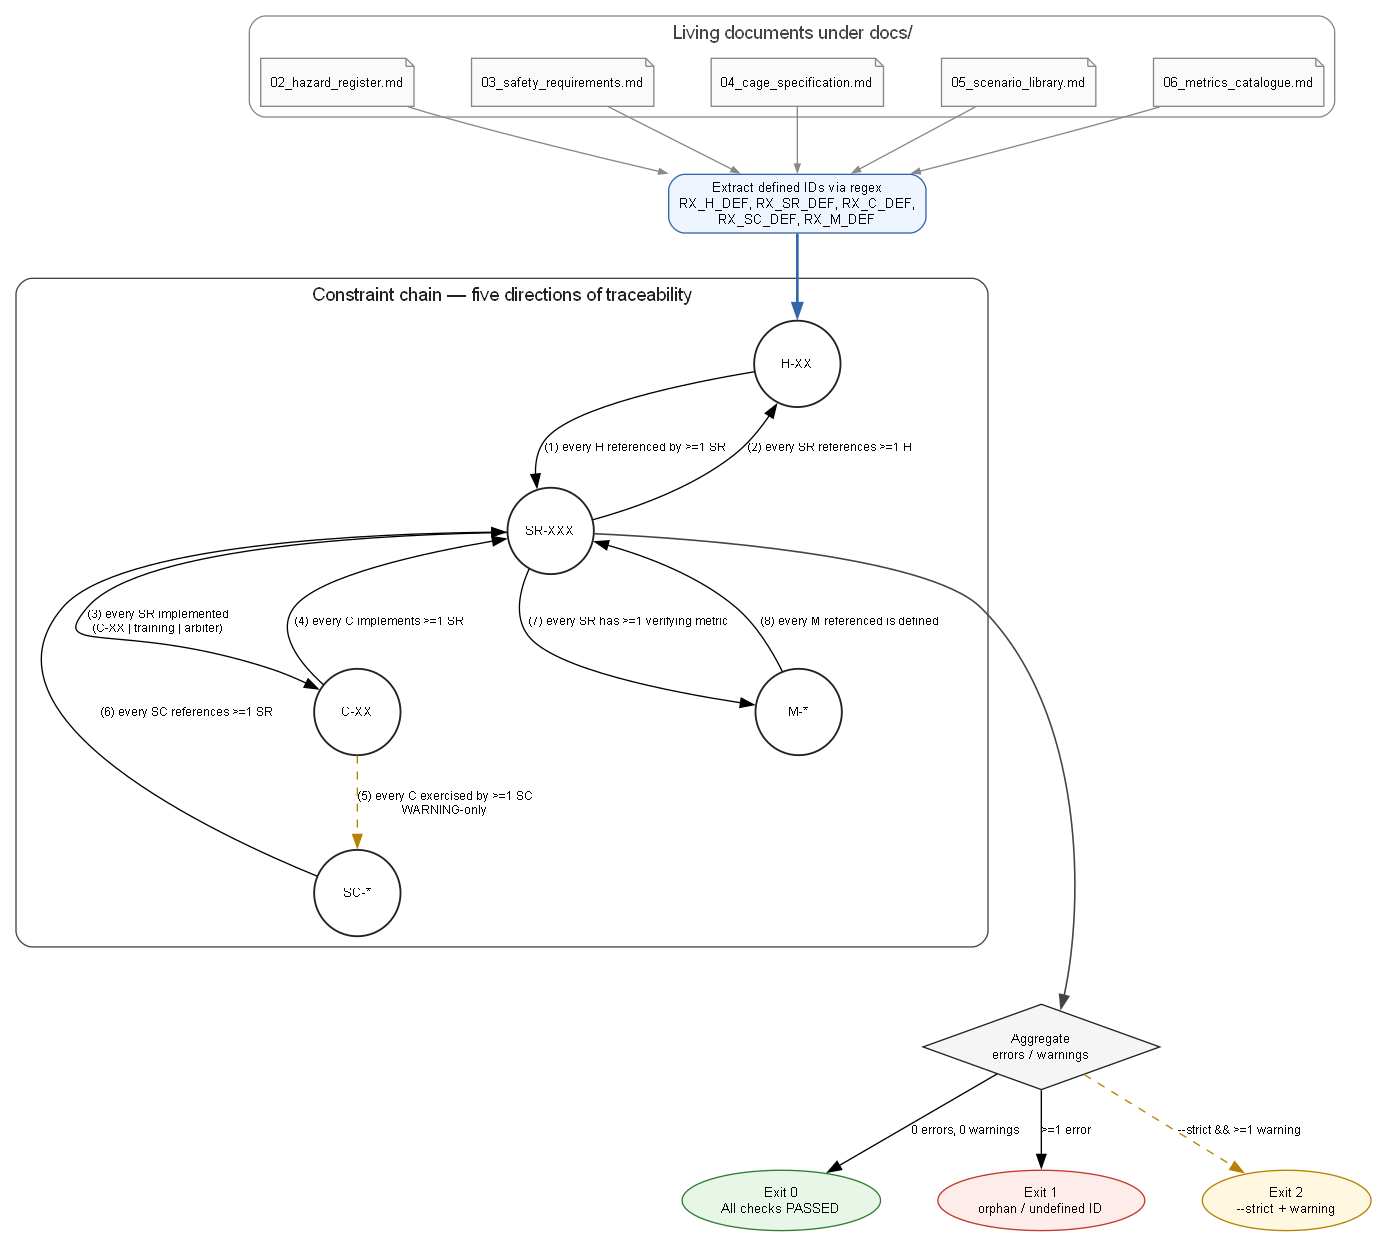
\includegraphics[width=0.76\widefigurewidth]{fig_3_2_check_traceability_flow.png}
  \caption[Flow of the traceability validator.]{Flow of the traceability checker, in four layers: loading the living documents; extracting identifiers with regular expressions over the headings; checking the chain of constraints over the graph \texttt{H ↔ SR ↔ C ↔ SC}, with the subgraph \texttt{SR ↔ M} attached to the requirements node; and combining the results into one of three outputs: all checks pass, orphan or invalid reference, or a warning in strict mode.}\label{fig:3.2}
\end{figure*}

This has an indirect but important effect on design. The constraint makes the hazard analysis easier, because from the very first requirement it forces the question \enquote{which rule will handle this?}. The result is requirements that are more practical and less abstract. The idea is close to the GSN patterns of AMLAS, but A4 goes one step further by making traceability something a tool can check, instead of a documentation practice that someone has to review.

\subsection{A5 — Bounded operational validation and gap measurement}
\label{sec:3.4.5}

\textbf{Problem.} The acceptance test assumes a pass/fail verdict against the stakeholders' requirements and, without saying it, assumes that test conditions represent real operating conditions. For a system trained in simulation this is false. The gap is a major risk, and passing a test in simulation does not mean the system is safe in the real world.

\textbf{Adaptation.} This level becomes Operational Validation, with two required parts. The first is scenario-based validation linked to requirements, with coverage metrics over the ODD. The second is an explicit, quantitative measurement of the gap between the training environment and the operating environment, for each metric and each relevant failure mode. The conclusion is no longer \enquote{the system is safe}. It becomes: \emph{the system meets the requirements under the conditions of ODD X, with a measured gap of Y compared with the training conditions, and with the following residual risks documented}.

\subsection{Summary}
\label{sec:3.4.6}

% layout: table*, fixed, \small, 164 of 165 mm
\begin{table*}[htbp]
\caption{The five adaptations to the classical V-Model.}\label{tab:3.2}
\small\setlength{\tabcolsep}{4pt}
\begin{tabular}{@{}>{\RaggedRight\arraybackslash}p{6.1mm}>{\RaggedRight\arraybackslash}p{28.0mm}>{\RaggedRight\arraybackslash}p{49.4mm}>{\RaggedRight\arraybackslash}p{47.4mm}>{\RaggedRight\arraybackslash}p{21.4mm}@{}}
  \toprule
  \tabhead{ID} & \tabhead{Adaptation} & \tabhead{Problem of the classical V} & \tabhead{Solution} & \tabhead{Artefact} \\
  \midrule
  A1 & Splitting the module design & The policy has no a priori specification & Cage Spec (classical) + Training Spec (meta-design) & Ch. 5 and 7 \\
  \addlinespace[2pt]
  A2 & Splitting the unit test & The policy cannot be unit tested in the classical way & Cage tests + statistical behavioural evaluation & Test suite + Ch. 8 \\
  \addlinespace[2pt]
  A3 & Runtime monitoring level & Static validation is not enough & Intervention logging as continuous evidence & Logging node + data \\
  \addlinespace[2pt]
  A4 & Required traceability & Orphans hide \enquote{emergent properties} & Two-way hard constraint \texttt{H↔SR↔C↔SC↔M} & Matrix + checker \\
  \addlinespace[2pt]
  A5 & Bounded validation with gap & The simulation test does not represent operation & Verdict with limits + measured gap & Ch. 9 and 10 \\
  \bottomrule
\end{tabular}
\end{table*}

\begin{figure*}[htbp]
  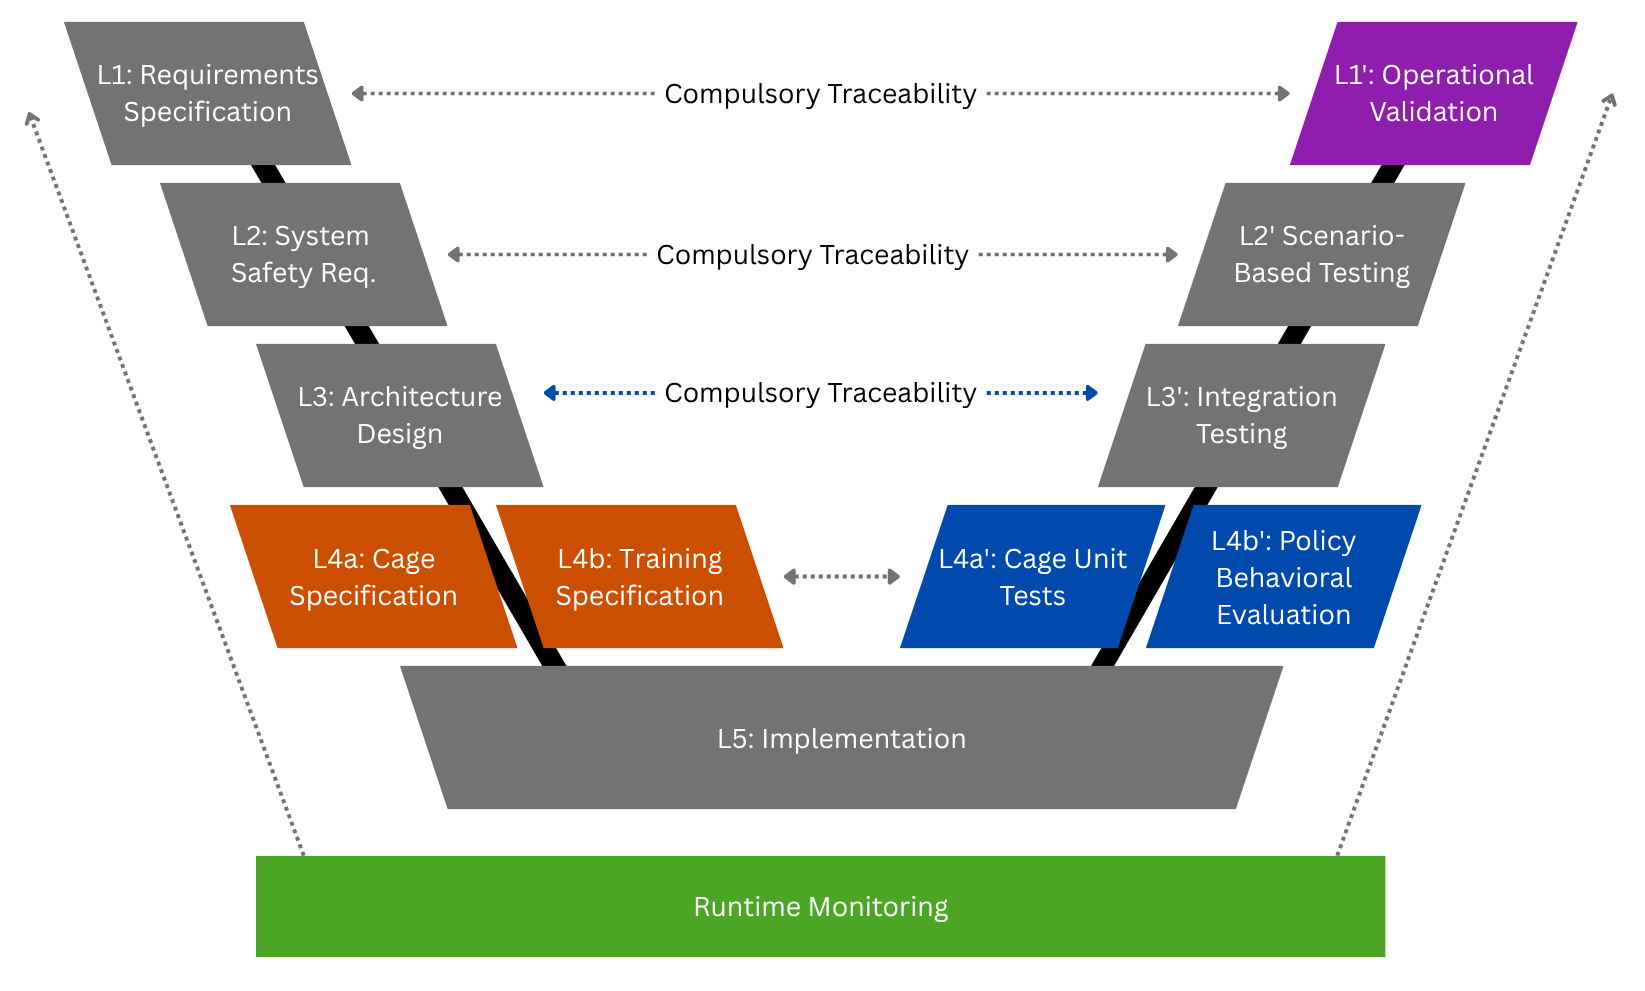
\includegraphics[width=0.77\widefigurewidth]{fig_3_3_adapted_v_model.png}
  \caption[Adapted V-Model.]{V-Model adapted to AI. Grey elements come from the classical V; coloured elements are new or changed by adaptations A1–A5.}\label{fig:3.3}
\end{figure*}

\section{Applying the framework to the case study}
\label{sec:3.5}

\subsection{System under study and architecture decision}
\label{sec:3.5.1}

The system is a 1:14 scale radio-controlled vehicle. Its main sensor is a single front camera, and it also has an inertial unit and a motor encoder, with onboard computing on a board that supports ROS2. It is developed on two platforms in parallel. One is simulated: Gazebo with native ROS2 integration, run through a gymnasium–\allowbreak{}Gazebo–\allowbreak{}ROS2 interface that reuses an environment the author built in earlier work. The other is physical: a closed track with controlled lighting.

One architecture decision matters for the methodology and not only for the system. At first, the project used an explicit modular split (perception, policy, cage, actuation and logging), with the learned component kept in a limited position. This followed the advice of Salay et al.~\cite{salay2017} to avoid ML at the architectural level and keep it at unit level. Later, the main system became an end-to-end camera version, where the policy is a CNN that learns perception and maps the image to an action.

This change is safe because the safety architecture stays the same. The cage is kept and works on its own deterministic lane estimator. This estimator is a classical vision pipeline, separate from the CNN, so it is neither ground truth nor a learned network. The pixels go into the policy, but the envelope works on a state that can be audited and is independent. The reasons for the original decision still hold. A1 holds because cage and policy are still different modules. A2 holds because the cage can be verified without the policy. A4 holds because the traceability chain does not change. The cost that was accepted is the other original reason: end-to-end learning needs more training, and Chapter~\ref{ch:07} plans for this. The state track is kept frozen as a control arm to isolate the cost of perception.

\subsection{Mapping the framework onto the case}
\label{sec:3.5.2}

% layout: table*, natural, \small, 149 of 165 mm
\begin{table*}[htbp]
\caption{Mapping of the framework onto the case study.}\label{tab:3.3}
\small\setlength{\tabcolsep}{4pt}
\begin{tabular}{@{}lll@{}}
  \toprule
  \tabhead{Level of the adapted V-Model} & \tabhead{Artefact in the case study} & \tabhead{Chapter} \\
  \midrule
  L1 — Stakeholder requirements & ODD + use case & 4 \\
  L2 — System safety requirements & \texttt{SR-001..SR-014} derived from the HARA & 4 \\
  L3 — Architectural design & ROS2 graph (perception, policy, cage, actuation, logging) & 5 \\
  L4a — Cage Specification & Rules \texttt{C-01..C-06} & 5 \\
  L4b — Training Specification & Reward, training ODD, hyperparameters, criteria & 7 \\
  L5 — Implementation & ROS2 cage node + trained policy & 6, 7 \\
  L4a' — Cage unit tests & Deterministic cage suite & 6 \\
  L4b' — Policy behavioural evaluation & Statistical analysis over the scenario library & 8 \\
  L3' — Integration test & Tests of the full chain & 6 \\
  L2' — Scenario-based test & Families \texttt{SC-NOM} / \texttt{SC-EDGE} / \texttt{SC-PERT} / \texttt{SC-FRONT} & 6, 8 \\
  L1' — Operational validation & Campaign + sim-to-real gap + verdict per requirement & 9, 10 \\
  Runtime monitoring (A3) & Logging node + intervention logs (across levels) & 5–10 \\
  \bottomrule
\end{tabular}
\end{table*}

This mapping is the first check that the framework can be put into practice. Every level of the V has an artefact, a chapter where it is developed, and a place in the traceability matrix.

\subsection{Phases}
\label{sec:3.5.3}

The project has seven phases in sequence. Each phase has defined deliverables and ends with a review gate\sidenote{A review gate is the check at the end of a phase. The project moves on only when the deliverables of the phase exist and the traceability checker reports no orphans.} that decides whether to move on. The phases are independent of the V-Model levels: one phase can produce artefacts for several levels, and one level can be built over several phases. In short: the first phase sets up the framework and the templates; the second produces the ODD, the hazard analysis and the requirements; the third develops the cage and its tests; the fourth defines the training specification and the scenario library; the fifth runs the training and the behavioural evaluation; the sixth deploys on the physical platform and measures the gap; and the last one collects the evidence and closes the matrix.

\begin{figure*}[htbp]
  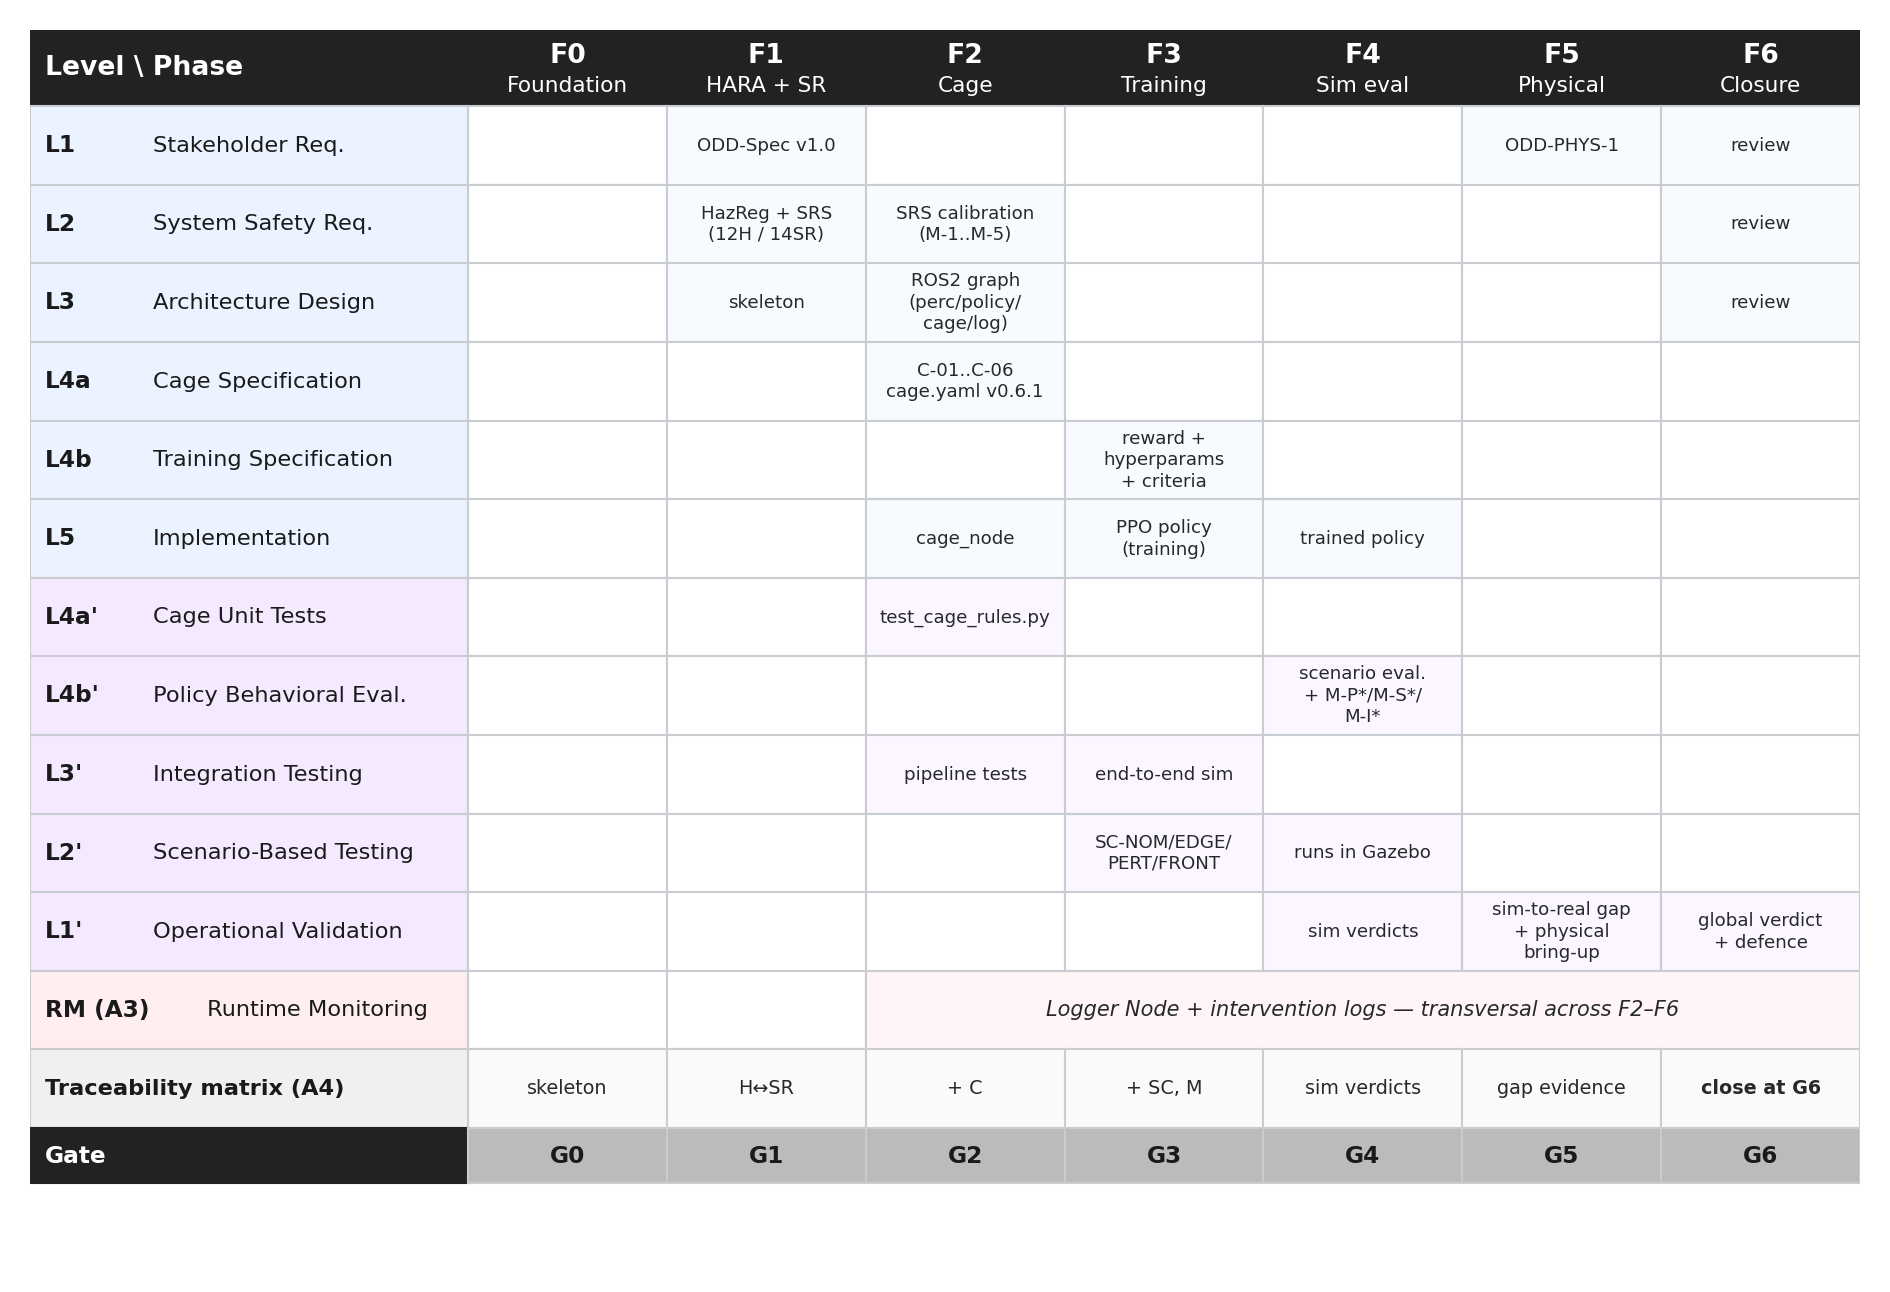
\includegraphics[width=0.77\widefigurewidth]{fig_3_4_project_phases.png}
  \caption[Project phases against the levels of the adapted V-Model.]{Project phases compared with the levels of the adapted V-Model. The monitoring band runs horizontally because it starts working as soon as the cage node exists and continues until the end. The traceability band shows how the chain \texttt{H ↔ SR ↔ C ↔ SC ↔ M} is completed phase by phase.}\label{fig:3.4}
\end{figure*}

One point is worth stressing, because it is where the framework stops being a proposal and becomes practice. A4 is fully active from the hazard analysis phase onwards. The checker runs on every change to the hazard register and the requirements specification. It requires every hazard to link to at least one requirement that reduces it, or to a documented accepted risk, and the other way round. From then on, the cycle \enquote{document $\rightarrow$ link $\rightarrow$ check} runs on every commit.

\section{Choice of tools}
\label{sec:3.6}

Each tool choice is explained against the alternatives that were rejected, so that decisions that would otherwise stay implicit leave a record that can be audited. Only the simulator is discussed here, because the methodology depends on it: it is the reference that adaptation A5 measures the gap against. The other choices (the learning algorithm and library, the physical platform, the measurement equipment and the reproducibility tools) are discussed in the same way in Appendix~\ref{app:C}, together with the clause-by-clause mapping to the standards. The middleware is not discussed separately because it comes with the simulator choice: native ROS2 integration is the first of the four reasons below.

\textbf{Simulator: Gazebo.} This choice is different from common practice, where CARLA is the reference. There are four reasons. \emph{Native ROS2 integration}: Gazebo is developed together with ROS and shares its basic building blocks without extra layers. The whole architecture is ROS2 by design, so running the simulator in the same graph removes possible failure points and makes it clearer where delays happen, which directly affects how accurate the integration metrics are. \emph{Reuse of earlier work}: the author already has an environment with the vehicle modelled and the track set up. Reusing it frees time for the methodological contribution, which is the real subject of the thesis. This fits the \emph{design science} approach, where the contribution is not the tool. \emph{An existing training interface}, which keeps algorithm, environment and system cleanly separated and so makes A1 easier. \emph{Low computing requirements}, which matters for an individual thesis without dedicated infrastructure.

The choice has two downsides that need to be stated. Gazebo's visual quality is lower than that of photorealistic engines, and for a camera-based policy this can mean a larger sim-to-real gap. Adaptation A5 exists to make this effect visible and to measure it, not to hide it. Also, most of the autonomous driving community uses CARLA, so there are no ready-made scenario libraries for Gazebo, and this project has to build its own.

Rejected alternatives: CARLA, the strongest option, because of its computing cost and because it needs a ROS2 bridge that brings its own problems; Highway-Env and similar tools, because they have no realistic sensors and use abstract observations, which makes them unsuitable for camera-based policies; LGSVL, which has been discontinued; and AirSim, which focuses on aerial vehicles and is no longer being developed.

\section{How the framework itself is evaluated}
\label{sec:3.7}

This section asks whether the methodology helped to build the system, not whether the system turned out to be useful. These are two different questions: a good framework can be applied to a modest system, and the other way round. The evaluation uses five criteria, each with an indicator that can be measured at the end:

\begin{enumerate}
  \item \textbf{Traceability integrity.} Indicator: orphans found by the checker in the last run. Success: zero.
  \item \textbf{Requirement coverage by evidence.} Indicator: percentage of requirements with a verdict supported by quantitative evidence. Success: 100\,\% have a verdict, even if it is negative or partial. An uncomfortable verdict is better than a missing one.
  \item \textbf{Hazard anticipation.} Indicator: how many of the hazards that actually appeared were predicted, compared with those that were not. Success: most observed hazards were predicted, and the unexpected ones can be audited and categorised.
  \item \textbf{Adoption cost.} Indicator: time spent on framework artefacts compared with purely technical artefacts. Success: the cost is in proportion to the benefit observed.
  \item \textbf{Usefulness of the matrix.} Indicator: technical changes where the matrix made the impact analysis faster. Success: documented cases where it clearly added value.
\end{enumerate}

The evaluation has three stated limits. It is internal to one project and has no control group, so conclusions are based on plausibility and not on controlled experiments. The author bias is limited but not removed. And the experimental period is short, while the benefits of A3 would show up over much longer periods.

\section{Relation to the standards}
\label{sec:3.8}

The framework does not replace the standards. It connects them. Each adaptation has a clear anchor in the standards, summarised in Table~\ref{tab:3.4}. The full clause-by-clause mapping is in Appendix~\ref{app:C}.

% layout: table*, fixed, \small, 164 of 165 mm
\begin{table*}[htbp]
\caption{Anchors in the standards for the five adaptations.}\label{tab:3.4}
\small\setlength{\tabcolsep}{4pt}
\begin{tabular}{@{}>{\RaggedRight\arraybackslash}p{46.0mm}>{\RaggedRight\arraybackslash}p{114.8mm}@{}}
  \toprule
  \tabhead{Adaptation} & \tabhead{Main anchor in the standards} \\
  \midrule
  A1 — Cage Spec + Training Spec & TR 5469 §7 (three-stage realisation principle); PAS 8800 (adapting the module design) \\
  \addlinespace[2pt]
  A2 — Cage tests + behavioural evaluation & TR 5469 (Class I / Class II elements); ISO 26262 Part 6 for the classical part \\
  \addlinespace[2pt]
  A3 — Runtime monitoring & SOTIF (static validation is not enough); operation phase as described by Wang et al.~\cite{wang2024} \\
  \addlinespace[2pt]
  A4 — Hard traceability & ISO 26262 Part 8 (requirements management); AMLAS (GSN patterns); UL 4600 (claim–\allowbreak{}argument–\allowbreak{}evidence) \\
  \addlinespace[2pt]
  A5 — Bounded validation + gap & SOTIF (unexpected conditions); UL 4600 (stated limits of the safety case) \\
  \bottomrule
\end{tabular}
\end{table*}

A note on the hazard analysis: the HARA used here is simpler than the one ISO 26262 prescribes. It is not done alongside the V but inside it, in exactly the place where the standard puts the output of the formal HARA. Chapter~\ref{ch:04} describes the simplifications and why they were made.

\section{Limitations of the methodology}
\label{sec:3.9}

It is better to state them clearly now, before the reader finds them in the final chapters.

\begin{itemize}
  \item \textbf{Construct validity is limited by having one case.} Generalisation relies on structure, not on evidence from several cases. Mitigation: Chapter~\ref{ch:12} separates the parts that can be reused from those that need to be rethought.
  \item \textbf{The simulation has only moderate visual quality.} All training happens in Gazebo, which can make the gap larger for the visual features the camera sees. Mitigation: A5 makes the gap visible and Chapter~\ref{ch:09} measures it. Repeating the experiment on a photorealistic simulator is a natural next step.
  \item \textbf{The five adaptations are not a complete list.} Others could be justified, for example a level for data engineering, following the data-centred approach of TR 5469 and AMLAS. Each of the five chosen here is justified, but there is no argument that they are the only possible ones.
  \item \textbf{The framework does not remove the author bias.} It only makes it open to audit.
\end{itemize}

\section{Next steps}
\label{sec:3.10}

With the framework defined, the next chapters apply it. Chapter~\ref{ch:04} covers the upper left branch of the V (operational domain, hazard analysis and requirement derivation) and produces the first artefacts that A4 checks as a hard constraint. After that, each chapter covers one level of the V and closes its link with the matching level on the right branch.

% GENERATED by md2tex.py from ../draft_v5_en/body/04_domain_hazards_requirements.md -- do not edit by hand.
% Change the Markdown and run `python md2tex.py`; edits here are overwritten.

\chapter{Operational domain, hazard analysis and safety requirements}
\label{ch:04}

\section{Purpose of the chapter}
\label{sec:4.1}

This chapter covers the upper left branch of the adapted V-Model. It contains the stakeholder requirements (level L1), expressed as the operational domain, and the system safety requirements (level L2), derived step by step from a hazard analysis. It is the first chapter where the framework of Chapter~\ref{ch:03} is no longer just a proposal: it produces artefacts that adaptation A4 checks as a hard constraint.

The official content of each artefact is kept in a version-controlled living document. This chapter shows the final form and the reasoning behind it. The full hazard register, with the root cause hypothesis and cross references for each entry, is in Appendix~\ref{app:A}. The full \emph{rationale} for each requirement, including how each threshold was derived, is in Appendix~\ref{app:B}. The complete operational domain specification, with its twelve open questions and how they were closed, is in Appendix~\ref{app:D}.

\section{Intended function and system requirements}
\label{sec:4.2}

The intended function is to keep the vehicle inside its lane along a closed track, under controlled conditions, without human help during the episode. The function is simple on purpose. The interest of the thesis is not in how advanced the function is, but in how rigorous the cycle that builds and validates it is.

Four system requirements come from this function, before any safety considerations. The vehicle must follow the lane with a limited lateral error. It must finish the route without stopping for no reason. It must run in real time within the stated control cycle. And it must log its behaviour so that the evidence can be reconstructed later. The first three are functional. The fourth comes directly from adaptation A3 and would not appear in a classical cycle.

\section{Operational domain}
\label{sec:4.3}

\subsection{Four domains}
\label{sec:4.3.1}

The operational domain is split into the four nested domains shown in Figure~\ref{fig:4.1}\sidenote{ODD, operational design domain: the conditions (layout, lighting, speed, latency) under which the system is designed to work. Outside it, no safety claim is made.}. Each one isolates one source of complexity. This makes it possible to link an observed change in safety or performance to one cause, and not to a mix of causes:

\begin{itemize}
  \item \textbf{\mbox{ODD-1} — nominal.} Reference layout, clean conditions, no stressors. This is the baseline.
  \item \textbf{\mbox{ODD-2} — adverse.} The same layout with stressors on the perception channel. On the camera track these are visual problems: glare, low light, motion blur, and worn or covered markings.
  \item \textbf{\mbox{ODD-3} — demanding layout.} A winding, tight layout in clean conditions, with a speed limit that depends on curvature.
  \item \textbf{\mbox{ODD-4} — combined.} The \mbox{ODD-3} layout combined with the \mbox{ODD-2} stressors.
\end{itemize}

\begin{figure*}[htbp]
  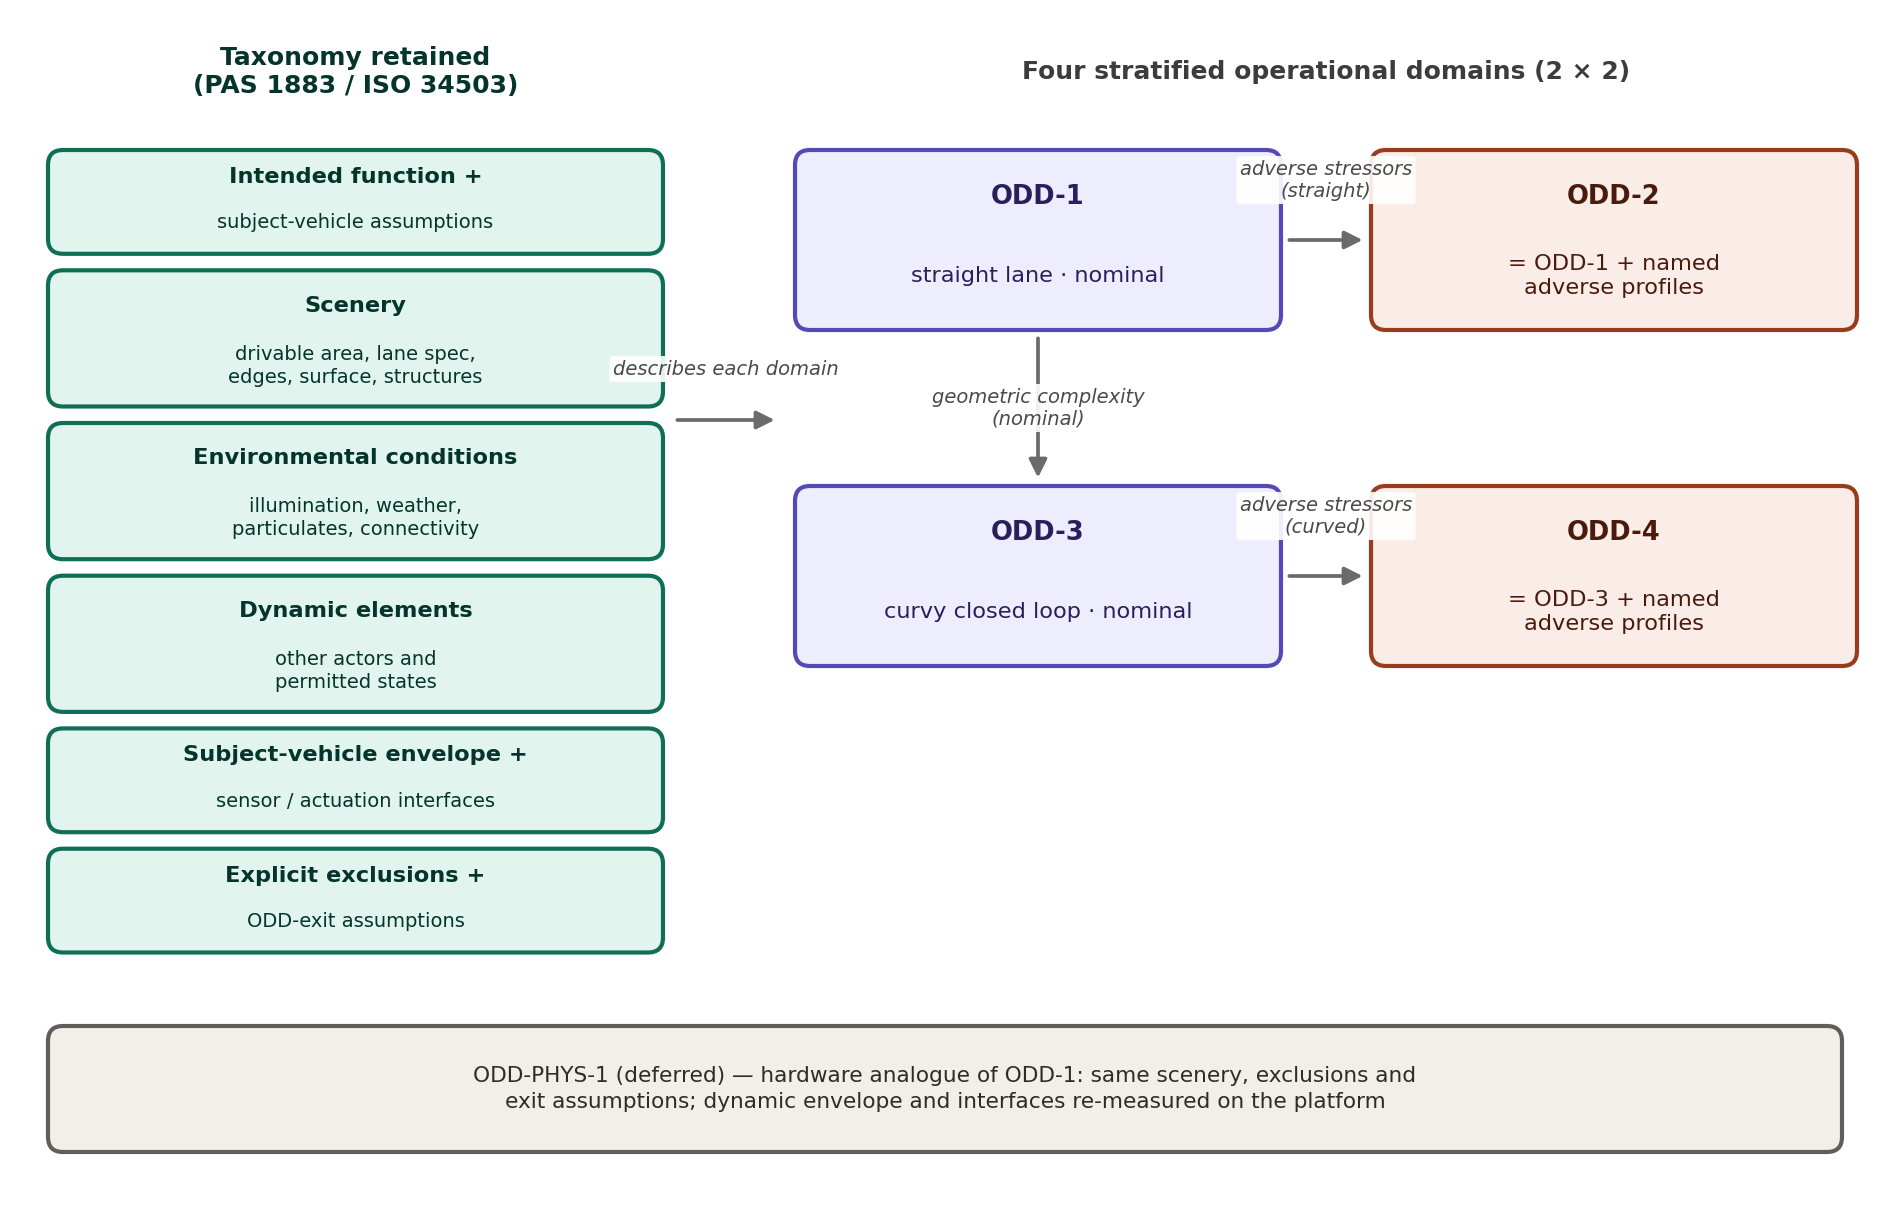
\includegraphics[width=0.93\widefigurewidth]{fig_4_1_odd_taxonomy.png}
  \caption[ODD taxonomy retained and the four stratified domains.]{The ODD taxonomy used and the four domains. On the left, the PAS 1883 / ISO 34503 dimensions used to describe each domain. On the right, the 2 $\times$ 2 split whose pairwise comparisons let Chapter~\ref{ch:08} link an effect to a single source of complexity: \mbox{ODD-1} against \mbox{ODD-2} isolates the stressors on straight track, \mbox{ODD-1} against \mbox{ODD-3} isolates the harder layout in clean conditions, and \mbox{ODD-3} against \mbox{ODD-4} adds stressors on curves.}\label{fig:4.1}
\end{figure*}

Each domain sets named parameters: lane and road width, friction coefficient, maximum curvature, speed range, control latency, and the size of the observation and the action. This way any later claim can point to a specific value and not to a vague description.

\subsection{Domain attributes and scenario stressors}
\label{sec:4.3.2}

One distinction is kept strictly throughout this work, because mixing the two often leads to wrong conclusions. A domain attribute defines where the system is \emph{allowed} to operate. A scenario stressor is a disturbance added inside that domain to trigger a specific failure mode. If a stressor inside the domain causes the vehicle to leave the lane, that is a system failure. If the same departure is caused by a starting condition outside the domain, it is not, and counting it as a failure would make the verdict invalid. This distinction is the basis for the \enquote{inside/outside the ODD} split that Chapter~\ref{ch:08} uses to read all its results.

\subsection{Physical domain}
\label{sec:4.3.3}

For deployment on the real platform, a matching domain is planned, as close as the hardware allows. It has the same scenario type, exclusions and exit hypotheses, but it differs in the vehicle's dynamic limits, the sensing and actuation interfaces, and the normal loop latency. One domain parameter, the maximum commanded lateral acceleration, cannot be measured in simulation at all, because there it would simply follow from the friction coefficient that the simulated world assumes. It stays open and explicitly waits for a physical calibration. It is the only domain question that this work leaves open, and it is marked as open instead of being estimated.

\section{Hazard analysis}
\label{sec:4.4}

\subsection{Procedure}
\label{sec:4.4.1}

The analysis follows the structure of a HARA as in ISO 26262\sidenote{HARA, hazard analysis and risk assessment: the ISO 26262 step that lists hazards, rates them and derives the safety goals that the requirements must meet.} (Figure~\ref{fig:4.2} shows the procedure as applied), with three simplifications that need to be stated. It is applied to one function and one element instead of a full vehicle. The operational situations come from the four domains instead of from a usage catalogue. And instead of assigning an integrity level, it uses a custom two-class criticality scale, which suits a scale vehicle with no consequences for people. These simplifications change the scope of the reasoning, not its structure: situation, hazard, severity, exposure, controllability, criticality, mitigation.

\begin{figure*}[htbp]
  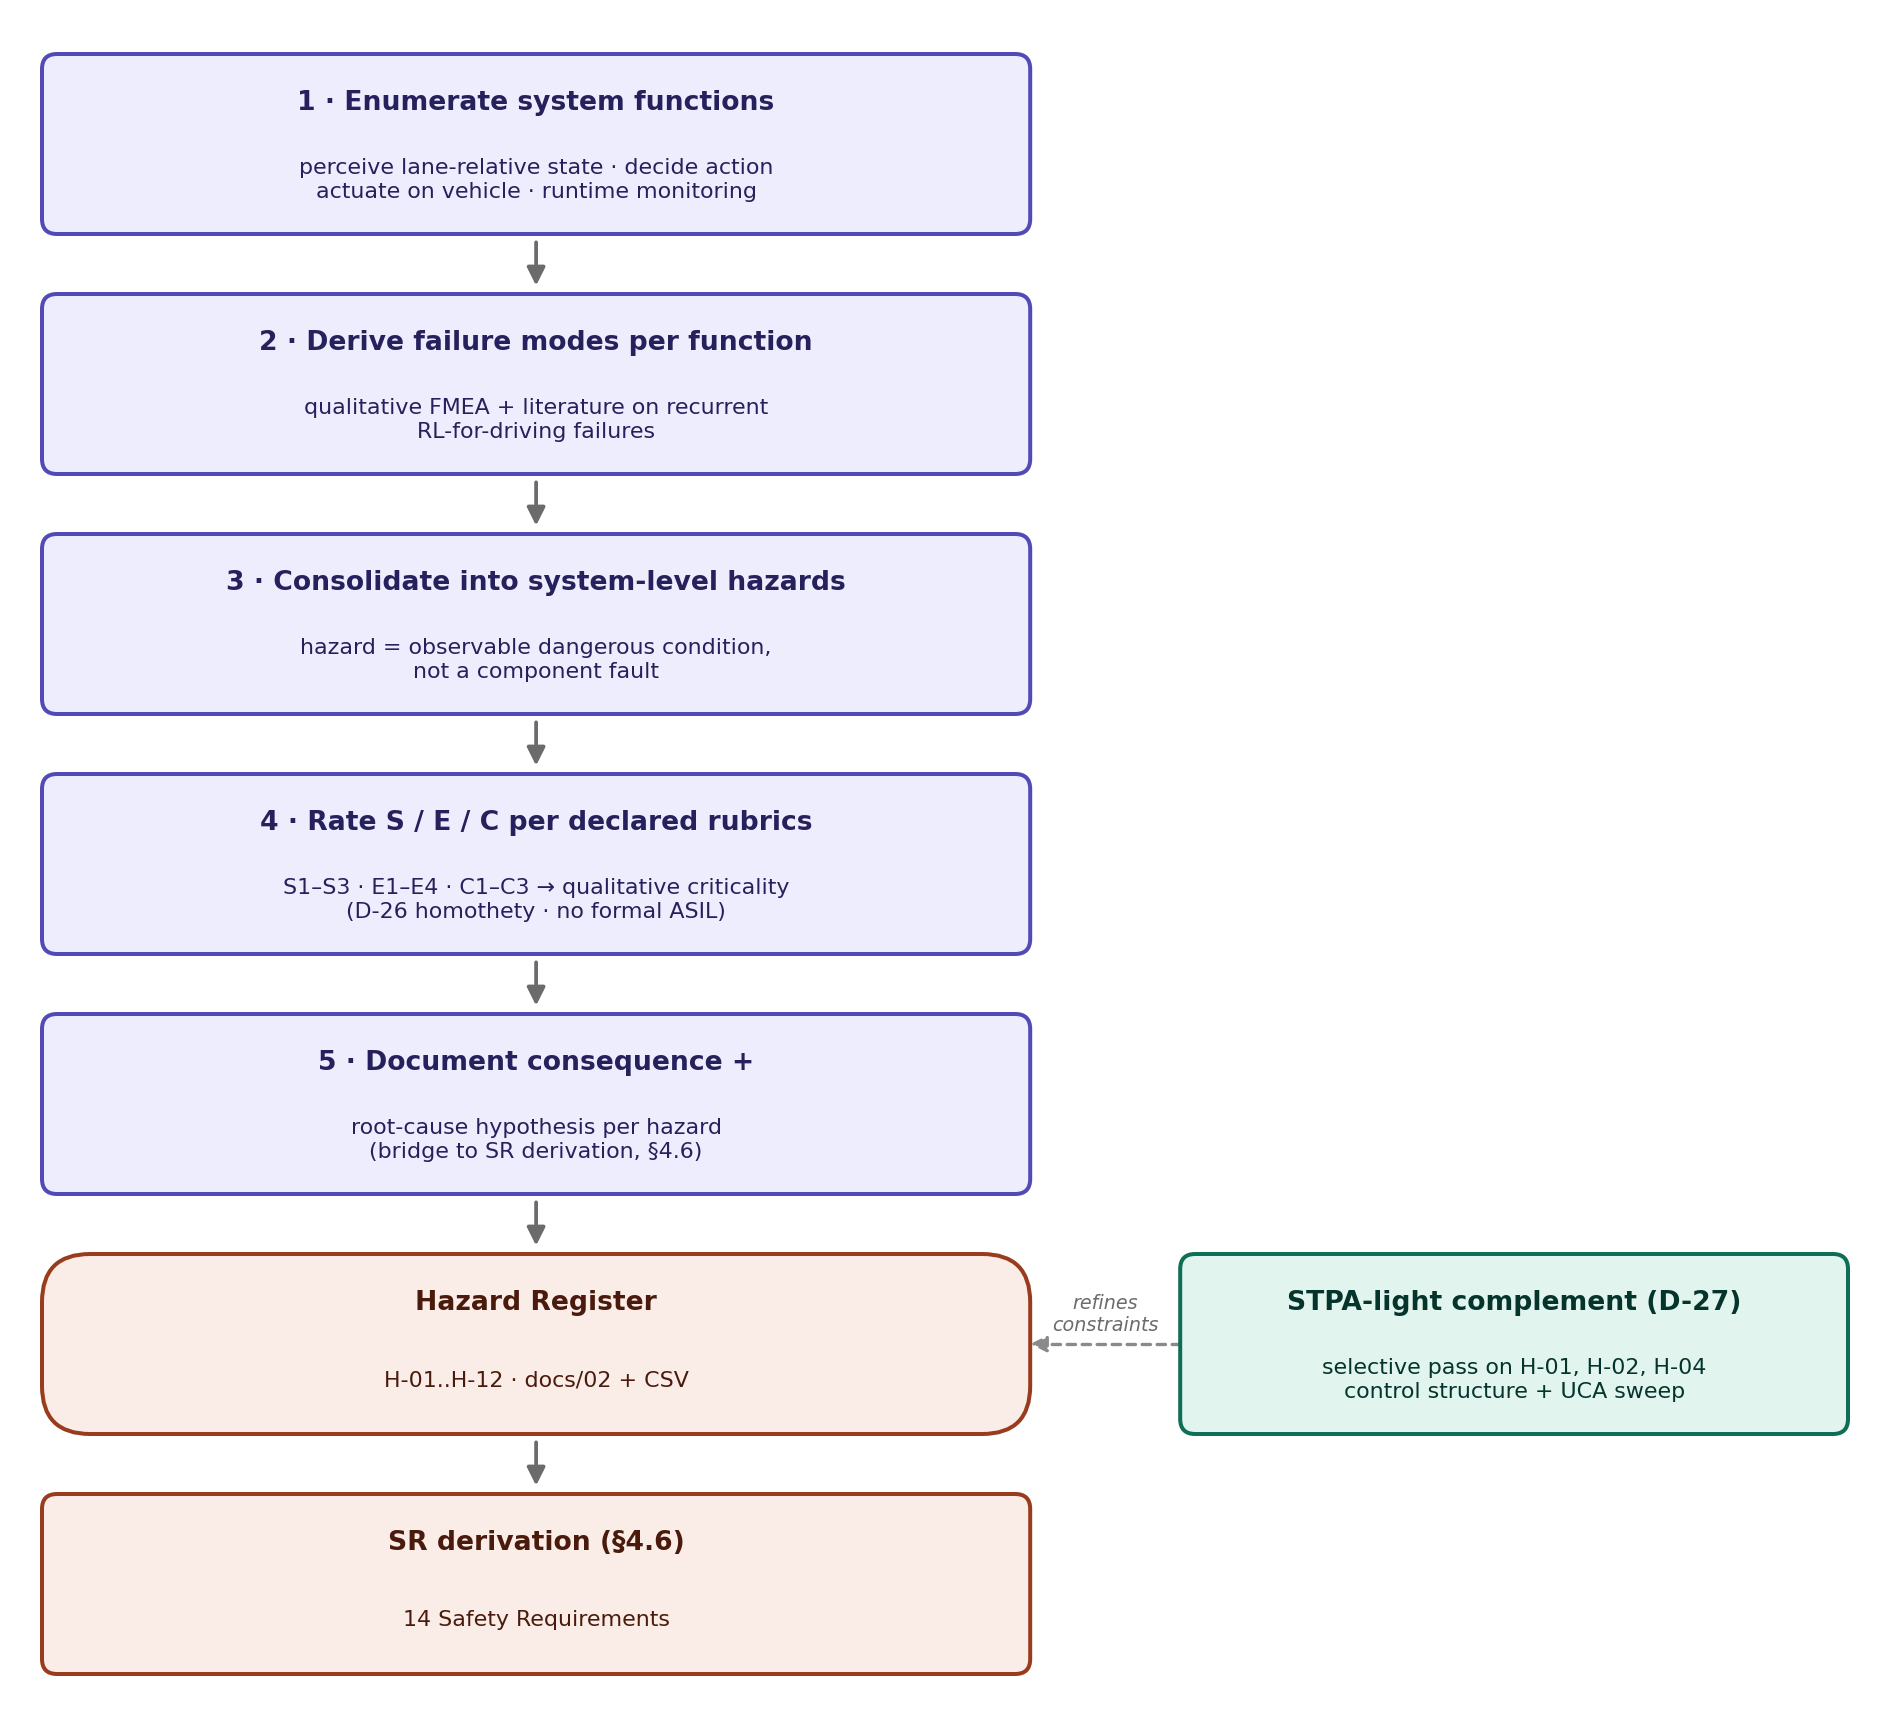
\includegraphics[width=0.90\widefigurewidth]{fig_4_2_hara_procedure.png}
  \caption[The HARA procedure as applied.]{The HARA procedure as applied: five steps from listing the functions to documenting the consequence and the root-cause hypothesis. A light systemic pass refines the constraints on selected hazards, and the output is the hazard register.}\label{fig:4.2}
\end{figure*}

Each hazard is rated on three axes with explicit scales\sidenote{The three ratings follow ISO 26262 Part 3, adapted to a 1:14 vehicle on a closed track. \S\ref{sec:C.2.7} explains what each level means here.}. Severity runs from S0, no injury, to S3, a serious consequence on the full-size equivalent. Exposure runs from E0 to E4, based on how often the situation happens inside the domain. Controllability runs from C0 to C3, based on how well the system or a supervisor can avoid the damage. Together they give the criticality, which decides whether the hazard needs a deterministic rule, a training constraint, or both.

\subsection{Hazard register}
\label{sec:4.4.2}

The register, summarised in Table~\ref{tab:4.1}, contains twelve hazards: nine at system level, shared by both tracks, and three specific to the camera track. The numbering is stable. Once an identifier is assigned it is never reused or renamed, even if the hazard is dropped in a later review. The table is the short version. The extended register, with the root cause hypothesis and the operational consequence of each entry, is in Appendix~\ref{app:A}.

% layout: table*, natural, \small, 138 of 165 mm
\begin{table*}[htbp]
\caption{Hazard register, short version (extended register in Appendix~\ref{app:A}).}\label{tab:4.1}
\small\setlength{\tabcolsep}{4pt}
\begin{tabular}{@{}llcccl@{}}
  \toprule
  \tabhead{ID} & \tabhead{Hazard} & \tabhead{S} & \tabhead{E} & \tabhead{C} & \tabhead{Criticality} \\
  \midrule
  \hz{01} & Unintended lateral departure from the lane & S3 & E3 & C2 & High \\
  \hz{02} & Divergent or oscillatory orientation error & S2 & E3 & C2 & Medium-high \\
  \hz{03} & Excessive speed for the local curvature & S3 & E2 & C1 & Medium-high \\
  \hz{04} & Unrecoverable compound state (heading + offset + speed) & S3 & E1 & C3 & High \\
  \hz{05} & Abrupt actuation command between consecutive cycles & S1 & E3 & C1 & Medium \\
  \hz{06} & Operation on a non-observable or corrupted state & S3 & E2 & C2 & High \\
  \hz{07} & Impossibility of performing a controlled stop & S3 & E1 & C1 & High \\
  \hz{08} & \emph{Stall} through reward exploitation & S2 & E3 & C2 & Medium-high \\
  \hz{09} & Conflict between cage rules under co-activation & S3 & E1 & C2 & Medium \\
  \hz{10} & Poor lane perception from degraded visual input & S3 & E3 & C2 & High \\
  \hz{11} & Loss of valid lane perception & S3 & E2 & C2 & High \\
  \hz{12} & Wrong detection by the cage estimator (plausible false lane) & S3 & E2 & C2 & High \\
  \bottomrule
\end{tabular}
\end{table*}

Three entries need a comment, because they would not appear in a classical analysis. \hz{08} is specific to the learned component. It is reward exploitation: the policy ends up doing nothing, or doing something harmful, because that earns more reward than normal lane following. \hz{09} is specific to the \emph{mitigation}. Two or more cage rules may fire in the same cycle. If their combined output is a command outside the safe envelope, the cage is no longer a guarantee and becomes a source of unsafe commands. Recording the hazards created by the safety mechanism itself is a basic matter of honesty, and Chapter~\ref{ch:08} shows that this was not just a formal precaution. \hz{12} is the camera-track version of the same idea: the cage estimator produces a lane that is false but looks plausible, and applies a wrong envelope over the real lane.

\subsection{Systemic analysis}
\label{sec:4.4.3}

For the most critical hazards, a light systemic analysis based on control theory is also carried out\sidenote{This is a light version of STPA, System-Theoretic Process Analysis, which looks for unsafe control actions in the whole loop instead of broken components.}. It looks at unsafe control actions in the whole loop, instead of failure modes of single components. It found two types of hazard that the component-based analysis had missed: hazards from acting on invalid information (an outdated process model) and hazards from not acting when action was needed. Both types were turned into requirements that are now part of the core of the cage. The pass is \emph{light}, and it is described that way: it does not build the full hierarchical control model and does not list all causal scenarios.

\section{Deriving the safety requirements}
\label{sec:4.5}

\subsection{Procedure and quality criteria}
\label{sec:4.5.1}

Each hazard is turned into one or more requirements using the procedure in Figure~\ref{fig:4.3}. There are four required criteria, and the document template enforces them. Falsifiability: the requirement is a measurable condition with a defined way to reach a verdict. Operability: it can be implemented by a concrete mechanism, such as a rule, a training constraint or a scenario test. Traceability: it points to at least one hazard and is pointed to by at least one rule and one scenario. Atomicity: it describes only one property.

\begin{figure*}[htbp]
  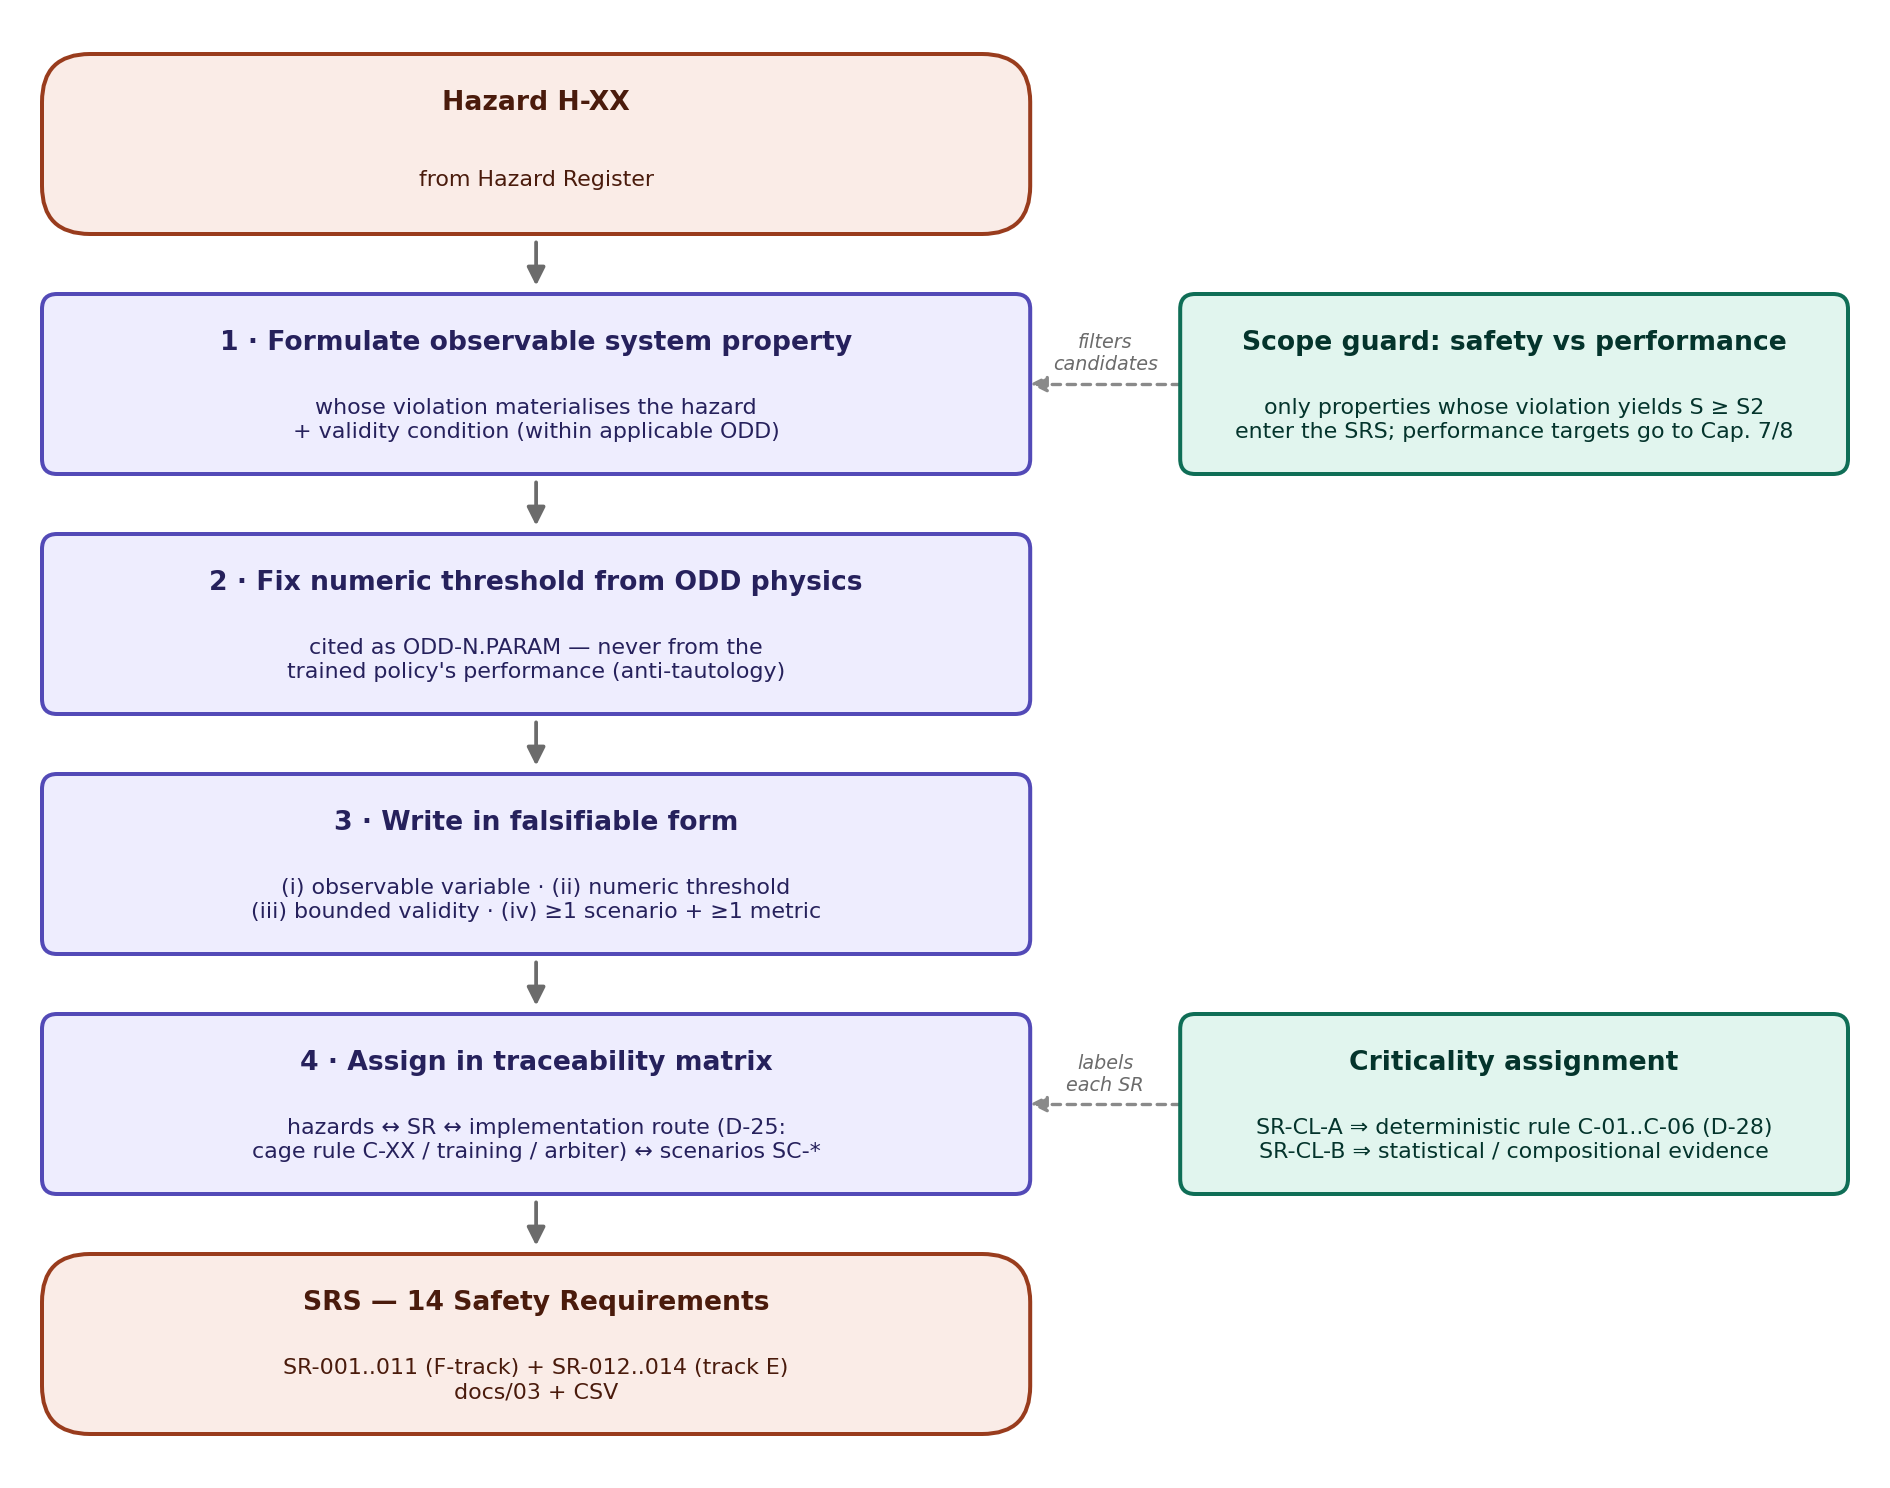
\includegraphics[width=0.90\widefigurewidth]{fig_4_3_sr_derivation.png}
  \caption[The safety-requirement derivation procedure.]{Deriving a safety requirement from a hazard, in four steps. Two guards make the result defensible. Thresholds are set from the physics of the ODD and never from how well the trained policy performed, which would be circular. And the criticality class decides how the requirement is implemented: every class A requirement ends up in a deterministic rule.}\label{fig:4.3}
\end{figure*}

Falsifiability is worth stressing, because everything else depends on it. A requirement like \enquote{the vehicle shall drive safely} cannot be falsified, so it cannot be verified or traced: no measurement could ever contradict it. Requiring a named threshold, a metric and a verdict procedure is what makes the traceability matrix a useful tool instead of a paperwork exercise.

\subsection{Requirements specification}
\label{sec:4.5.2}

The register has fourteen requirements. Table~\ref{tab:4.2} shows the short version. The full \emph{rationale} for each one, including how each threshold was derived and a discussion of the values marked provisional until physical calibration, is in Appendix~\ref{app:B}.

% layout: table*, fixed, \small, 164 of 165 mm
\begin{table*}[htbp]
\caption{Safety requirements specification, short version (full rationale in Appendix~\ref{app:B}).}\label{tab:4.2}
\small\setlength{\tabcolsep}{4pt}
\begin{tabular}{@{}>{\RaggedRight\arraybackslash}p{10.6mm}>{\RaggedRight\arraybackslash}p{61.2mm}>{\RaggedRight\arraybackslash}p{27.1mm}>{\RaggedRight\arraybackslash}p{13.4mm}>{\RaggedRight\arraybackslash}p{26.5mm}>{\centering\arraybackslash}p{10.6mm}@{}}
  \toprule
  \tabhead{ID} & \tabhead{Requirement (short form)} & \tabhead{Main threshold} & \tabhead{Hazard} & \tabhead{Implementation} & \tabhead{Class} \\
  \midrule
  \sr{001} & Bounded lateral offset inside the ODD & \texttt{d\_max = 0.16 m} & \hz{01} & \cagerule{01} & A \\
  \sr{002} & Bounded orientation error & \texttt{θ\_max = 25°} & \hz{02} & \cagerule{02} & A \\
  \sr{003} & Projected time to lane departure above a minimum & \texttt{t\_min = 1.0 s} & \hz{01}, \hz{02} & \cagerule{03} & A \\
  \sr{004} & Speed under a curvature-dependent ceiling & \texttt{0.25–0.5 m/s} & \hz{03} & \cagerule{04} & A \\
  \sr{005} & Transition to emergency mode under a compound \emph{trigger} & \texttt{θ\_warn 20°}, \texttt{d\_warn 0.12 m} & \hz{04}, \hz{07} & \cagerule{05} & A \\
  \sr{006} & Bounded command variation between cycles & \texttt{δ\_max = 0.15} & \hz{05} & \cagerule{06} & B \\
  \sr{007} & Emergency on a stale or out-of-range observation & \texttt{staleness ≤ 200 ms} & \hz{06} & \cagerule{05} & A \\
  \sr{008} & Controlled stop under an external signal & \texttt{t\_stop ≤ 1.7 s} & \hz{07} & \cagerule{05} & A \\
  \sr{009} & Minimum longitudinal progress (\emph{liveness}) & \texttt{Δs ≥ 0.10 m / 2 s} & \hz{08} & training & B \\
  \sr{010} & Consistent composition of co-active rules & joint envelope & \hz{09} & arbitration & B \\
  \sr{011} & Bounded heading variance & \texttt{σ\_θ ≤ 5°} & \hz{02} & \cagerule{06} + training & B \\
  \sr{012} & Lane following under degraded visual input & reuses \texttt{d\_max}, \texttt{θ\_max} & \hz{10} & \cagerule{01}/\allowbreak{}02/03 + training & A \\
  \sr{013} & Controlled stop on loss of perception & \texttt{≤ 200 ms} & \hz{11} & \cagerule{05} & A \\
  \sr{014} & Do not impose rules on an implausible estimate & plausibility tolerance & \hz{12} & \cagerule{05} & A \\
  \bottomrule
\end{tabular}
\end{table*}

One threshold in the table needs a note, because it is the only one the implementation changes. \sr{007} sets the maximum age of the state observation at \texttt{200 ms}, which is four cycles of the control loop at 20 Hz. The matching \cagerule{05} trigger runs at 10 Hz on the camera track and uses \texttt{0.5 s}. This is the same tolerance expressed in cycles (five), not a weaker requirement. The equivalence is recorded in the parameter file and in Appendix~\ref{app:D}. It is pointed out here so that the reader does not see a contradiction where there is only a stated change of parameters.

\subsection{Criticality classes}
\label{sec:4.5.3}

The requirements are split into two classes\sidenote{In the tables, A and B stand for the classes \texttt{SR-CL-A} and \texttt{SR-CL-B}. Only a failed class A requirement can make the global verdict fail.}, which affect the global verdict differently. Class A contains the requirements that express actual safety conditions. If one of them is violated, the global verdict of the campaign is invalid. Class B contains requirements for desirable quality properties, such as smoothness, no oscillation, \emph{liveness} and consistent rule composition. Their violation is reported, but it does not block the verdict.

This split is not a way out. It makes it possible to report an unmet requirement honestly without having to call a system unsafe when all its safety conditions are met. Chapter~\ref{ch:08} uses this distinction exactly once, and does so openly and with a reason.

\section{Two-way traceability matrix}
\label{sec:4.6}

The matrix is where A4 becomes concrete. It records the full chain \texttt{Hazard → Requirement → Rule → Scenario → Metric → Evidence → Verdict} and is kept in two forms: a readable table, and a machine-readable version that the checker uses.

In this chapter the matrix covers only its first part: the links between hazards and requirements. Every hazard in the register has at least one requirement that reduces it, and every requirement comes from at least one hazard, with no orphans in either direction. Two hazards, \hz{01} and \hz{02}, are covered by more than one requirement, because each can happen in more than one way. \hz{01} is covered by a hard offset limit and also by the predictive time-to-departure check. \hz{02} is covered by a limit on magnitude and a limit on variance, which cover the divergent and the oscillating versions of the same hazard.

The checker applies eight coverage constraints and fails the review gate if any of them is broken. The complete matrix, including the parts filled in by later chapters and the final verdicts, is in Appendix~\ref{app:F}.

\section{Limitations of the analysis}
\label{sec:4.7}

\begin{itemize}
  \item \textbf{Limited scope of the hazard analysis.} The HARA covers lane following on a scale platform. Neither the operational situations nor the severity scales can be used for a road vehicle without review.
  \item \textbf{Severities by analogy.} Severities are set by comparison with a real vehicle, not by measuring physical consequences on the scale platform. This is a stated convention, not a measurement.
  \item \textbf{Light systemic pass.} The control-theory analysis is not complete. It was run on the most critical hazards and found two new types, but the catalogue cannot be called closed.
  \item \textbf{Provisional thresholds.} Several thresholds are marked provisional until they are calibrated on the physical platform. The framework requires this status to be visible in the artefact itself, not left unstated, and the process to resolve it is defined: measure, update the parameter file, version it, re-run the affected scenarios and record the change.
  \item \textbf{Completeness cannot be proved.} No procedure can prove that the hazard catalogue is complete. What is claimed, and checked automatically, is that no identified hazard is left without mitigation and without evidence.
\end{itemize}

With the domain defined, the hazards listed and the requirements derived, Chapter~\ref{ch:05} moves to the design level: the system architecture and the specification of the cage that has to enforce these requirements at runtime.

% GENERATED by md2tex.py from ../draft_v5_en/body/05_architecture_and_cage.md -- do not edit by hand.
% Change the Markdown and run `python md2tex.py`; edits here are overwritten.

\chapter{Architectural design and cage specification}
\label{ch:05}

\section{Purpose of the chapter}
\label{sec:5.1}

This chapter covers two levels: architectural design (L3) and module specification in its classical form (L4a). It produces the first artefact where adaptation A1 becomes concrete: the Cage Specification. This is a deterministic, modular specification written in the traditional way, unlike the process specification that Chapter~\ref{ch:07} writes for the policy.

The chapter covers six things: the design idea behind the safety envelope, the conceptual problems that appear when building it, how the rules are derived from the requirements, the design of each rule, the version-controlled parameters, and the ROS2 architecture that runs it. The full parameter specification, with the numerical derivation of each threshold and its calibration status, is in Appendix~\ref{app:E}.

\section{Design idea: the cage as a runtime shield}
\label{sec:5.2}

\subsection{Choice of mechanism}
\label{sec:5.2.1}

As Chapter~\ref{ch:02} showed, there are four families of mechanisms for making a learned policy safe. This thesis uses the runtime shield as the main mechanism\sidenote{Runtime means that the check happens while the system runs, in every control cycle, not once before deployment.}, for three reasons.

The first reason is verifiability. A cage made of hand-written rules is a classical component. It can be unit tested deterministically, analysed statically and inspected. In TR 5469 terms (used by analogy, since the TR classifies AI technology), it matches Class I, while the policy is at best Class II. This difference is what lets the combined system keep a core that can be verified.

The second reason is independence from training. A guarantee that comes from changing the learning objective is statistical and depends on the training distribution. A guarantee that comes from runtime filtering depends on the state observed in each cycle, no matter how the policy was trained. So it still holds if the policy is retrained, replaced or gets worse.

The third reason is that it fits the framework. As a side effect of how it works, the shield produces an intervention log, and that log is exactly the evidence the runtime monitoring level (A3) needs. The cage is not only a safety mechanism. It is also the tool that measures how the policy behaves.

\subsection{Scope and limitations of the cage}
\label{sec:5.2.2}

Three clarifications help avoid reading too much into it. The cage is not a controller. It does not create behaviour; it corrects unsafe commands. If the policy drives well, the cage should stay inactive, and Chapter~\ref{ch:08} shows that this is what happens under clean nominal conditions. The cage is not a formal guarantee. Its rules are heuristics with thresholds taken from the requirements, not invariants proved on a dynamic model. It gives containment that can be measured, not proof. And the cage does not remove the need to train well. It is the last line of defence, not the first, and a system whose safety depended completely on the cage would be a badly trained system. Chapter~\ref{ch:08} forces an uncomfortable correction to this last claim.

\section{Design problems}
\label{sec:5.3}

Building an envelope of rules brings up six problems. They are design problems, not implementation problems, and solving them explicitly is part of what this chapter contributes.

\textbf{Priority and order between rules.} Several rules can fire in the same cycle on the same actuation channel. The chosen solution is a fixed, declared evaluation order. The rate limiter comes first, so it limits the raw command before any safety rule looks at it. Emergency mode comes last, because it must be able to override any earlier correction. In between, the lateral limit rule runs after the heading rule, so the harder limit on the more critical variable has the final say among the operational rules.

\textbf{Design of the correction.} A correction can be added to the policy's command or replace it. Replacing is chosen, so that policy and cage do not compete in the same space and produce a sum that neither intended. The size of the correction depends on how far the value is past the threshold, not a fixed amount. A constant correction would create jumps at the activation boundary.

\textbf{Reactive and predictive rules.} Rules that look at the current state always act late: by the time the offset reaches the threshold, the dynamics are already in trouble. So a predictive rule is added. It projects the state over a short horizon and acts on the estimated time to lane departure\sidenote{Also called TTLC, time to lane crossing: how long the vehicle would take to reach the lane boundary if it kept its current lateral motion.}. The two types work together: the reactive rule limits the present, and the predictive rule buys extra margin.

\textbf{Hysteresis and avoiding flickering.} A single threshold makes a rule switch on and off repeatedly around that value, and the resulting oscillating command is a hazard in itself. Every rule with a threshold therefore has a hysteresis band.\sidenote{With hysteresis a rule switches on above one threshold and off only below a lower one. The gap stops it from flickering when the value sits near the limit.} It switches on above one value and off below a lower one, and it remembers its state between cycles.

\textbf{Saturation and conflicts.} The combined corrections can go beyond the physical range of the actuator. Saturation is applied at the end of the chain, on the combined command, and not rule by rule. This keeps the result predictable no matter how many rules acted.

\textbf{Emergency mode and state validity.} Emergency mode has an entry condition based on a compound \emph{trigger}, a deterministic behaviour (braking at a minimum rate with steering frozen), and an explicit exit. Its triggers include the unrecoverable compound state, but also cases where the state itself is not valid: an old observation, fields outside a plausible range, or loss of perception. This last group is the system's chain of trust. If the cage cannot trust the state it sees, the safe response is not to correct the command but to stop the vehicle in a controlled way.

\section{From requirements to rules}
\label{sec:5.4}

Requirements are mapped to rules with an explicit procedure. For each requirement, three things are identified: the observable variable that expresses its condition, the mechanism that can keep that variable within limits, and the actuation channel to act on. Sometimes no such mechanism exists without going against the idea of the cage. This is the case for \emph{liveness}: a rule that forced positive throttle would be creating behaviour instead of correcting it. In that case the requirement is implemented at another level, and this is stated.

% layout: table*, fixed, \small, 164 of 165 mm
\begin{table*}[htbp]
\caption{Traceability from requirements to cage rules.}\label{tab:5.1}
\small\setlength{\tabcolsep}{4pt}
\begin{tabular}{@{}>{\RaggedRight\arraybackslash}p{29.2mm}>{\RaggedRight\arraybackslash}p{51.4mm}>{\RaggedRight\arraybackslash}p{41.4mm}>{\RaggedRight\arraybackslash}p{33.1mm}@{}}
  \toprule
  \tabhead{Requirement} & \tabhead{Rule} & \tabhead{Observed variable} & \tabhead{Channel} \\
  \midrule
  \sr{001} & \cagerule{01} — hard lateral limit & lateral offset & steering \\
  \addlinespace[2pt]
  \sr{002} & \cagerule{02} — heading error limit & heading error & steering \\
  \addlinespace[2pt]
  \sr{003} & \cagerule{03} — predictive time-to-departure limit & projected time to crossing & steering \\
  \addlinespace[2pt]
  \sr{004} & \cagerule{04} — speed ceiling & speed and local curvature & throttle \\
  \addlinespace[2pt]
  \sr{005}, \sr{007}, \sr{008}, \sr{013}, \sr{014} & \cagerule{05} — emergency mode & compound state, validity, estimator health & both \\
  \addlinespace[2pt]
  \sr{006}, \sr{011} & \cagerule{06} — rate limiter & command variation between cycles & both \\
  \addlinespace[2pt]
  \sr{009} & — & — & training constraint \\
  \addlinespace[2pt]
  \sr{010} & — & — & arbitration property of the chain \\
  \addlinespace[2pt]
  \sr{012} & \cagerule{01}, \cagerule{02}, \cagerule{03} over the estimated state & estimated offset and heading & steering \\
  \bottomrule
\end{tabular}
\end{table*}

Three comments. First, six rules cover fourteen requirements, because one rule can implement several requirements and one requirement can need several rules. Second, two requirements are not implemented by any rule. The framework makes this visible in the matrix and states the type of implementation instead, which is a training constraint in one case and an arbitration property in the other. Naming the type is more honest than inventing a rule that would cover them only formally. Third, the camera-track requirements do not add new rules. They reuse the existing rules on a state that comes from a different source. This is a design result in itself: the cage does not care where the state comes from.

\section{The six rules}
\label{sec:5.5}

\begin{figure*}[htbp]
  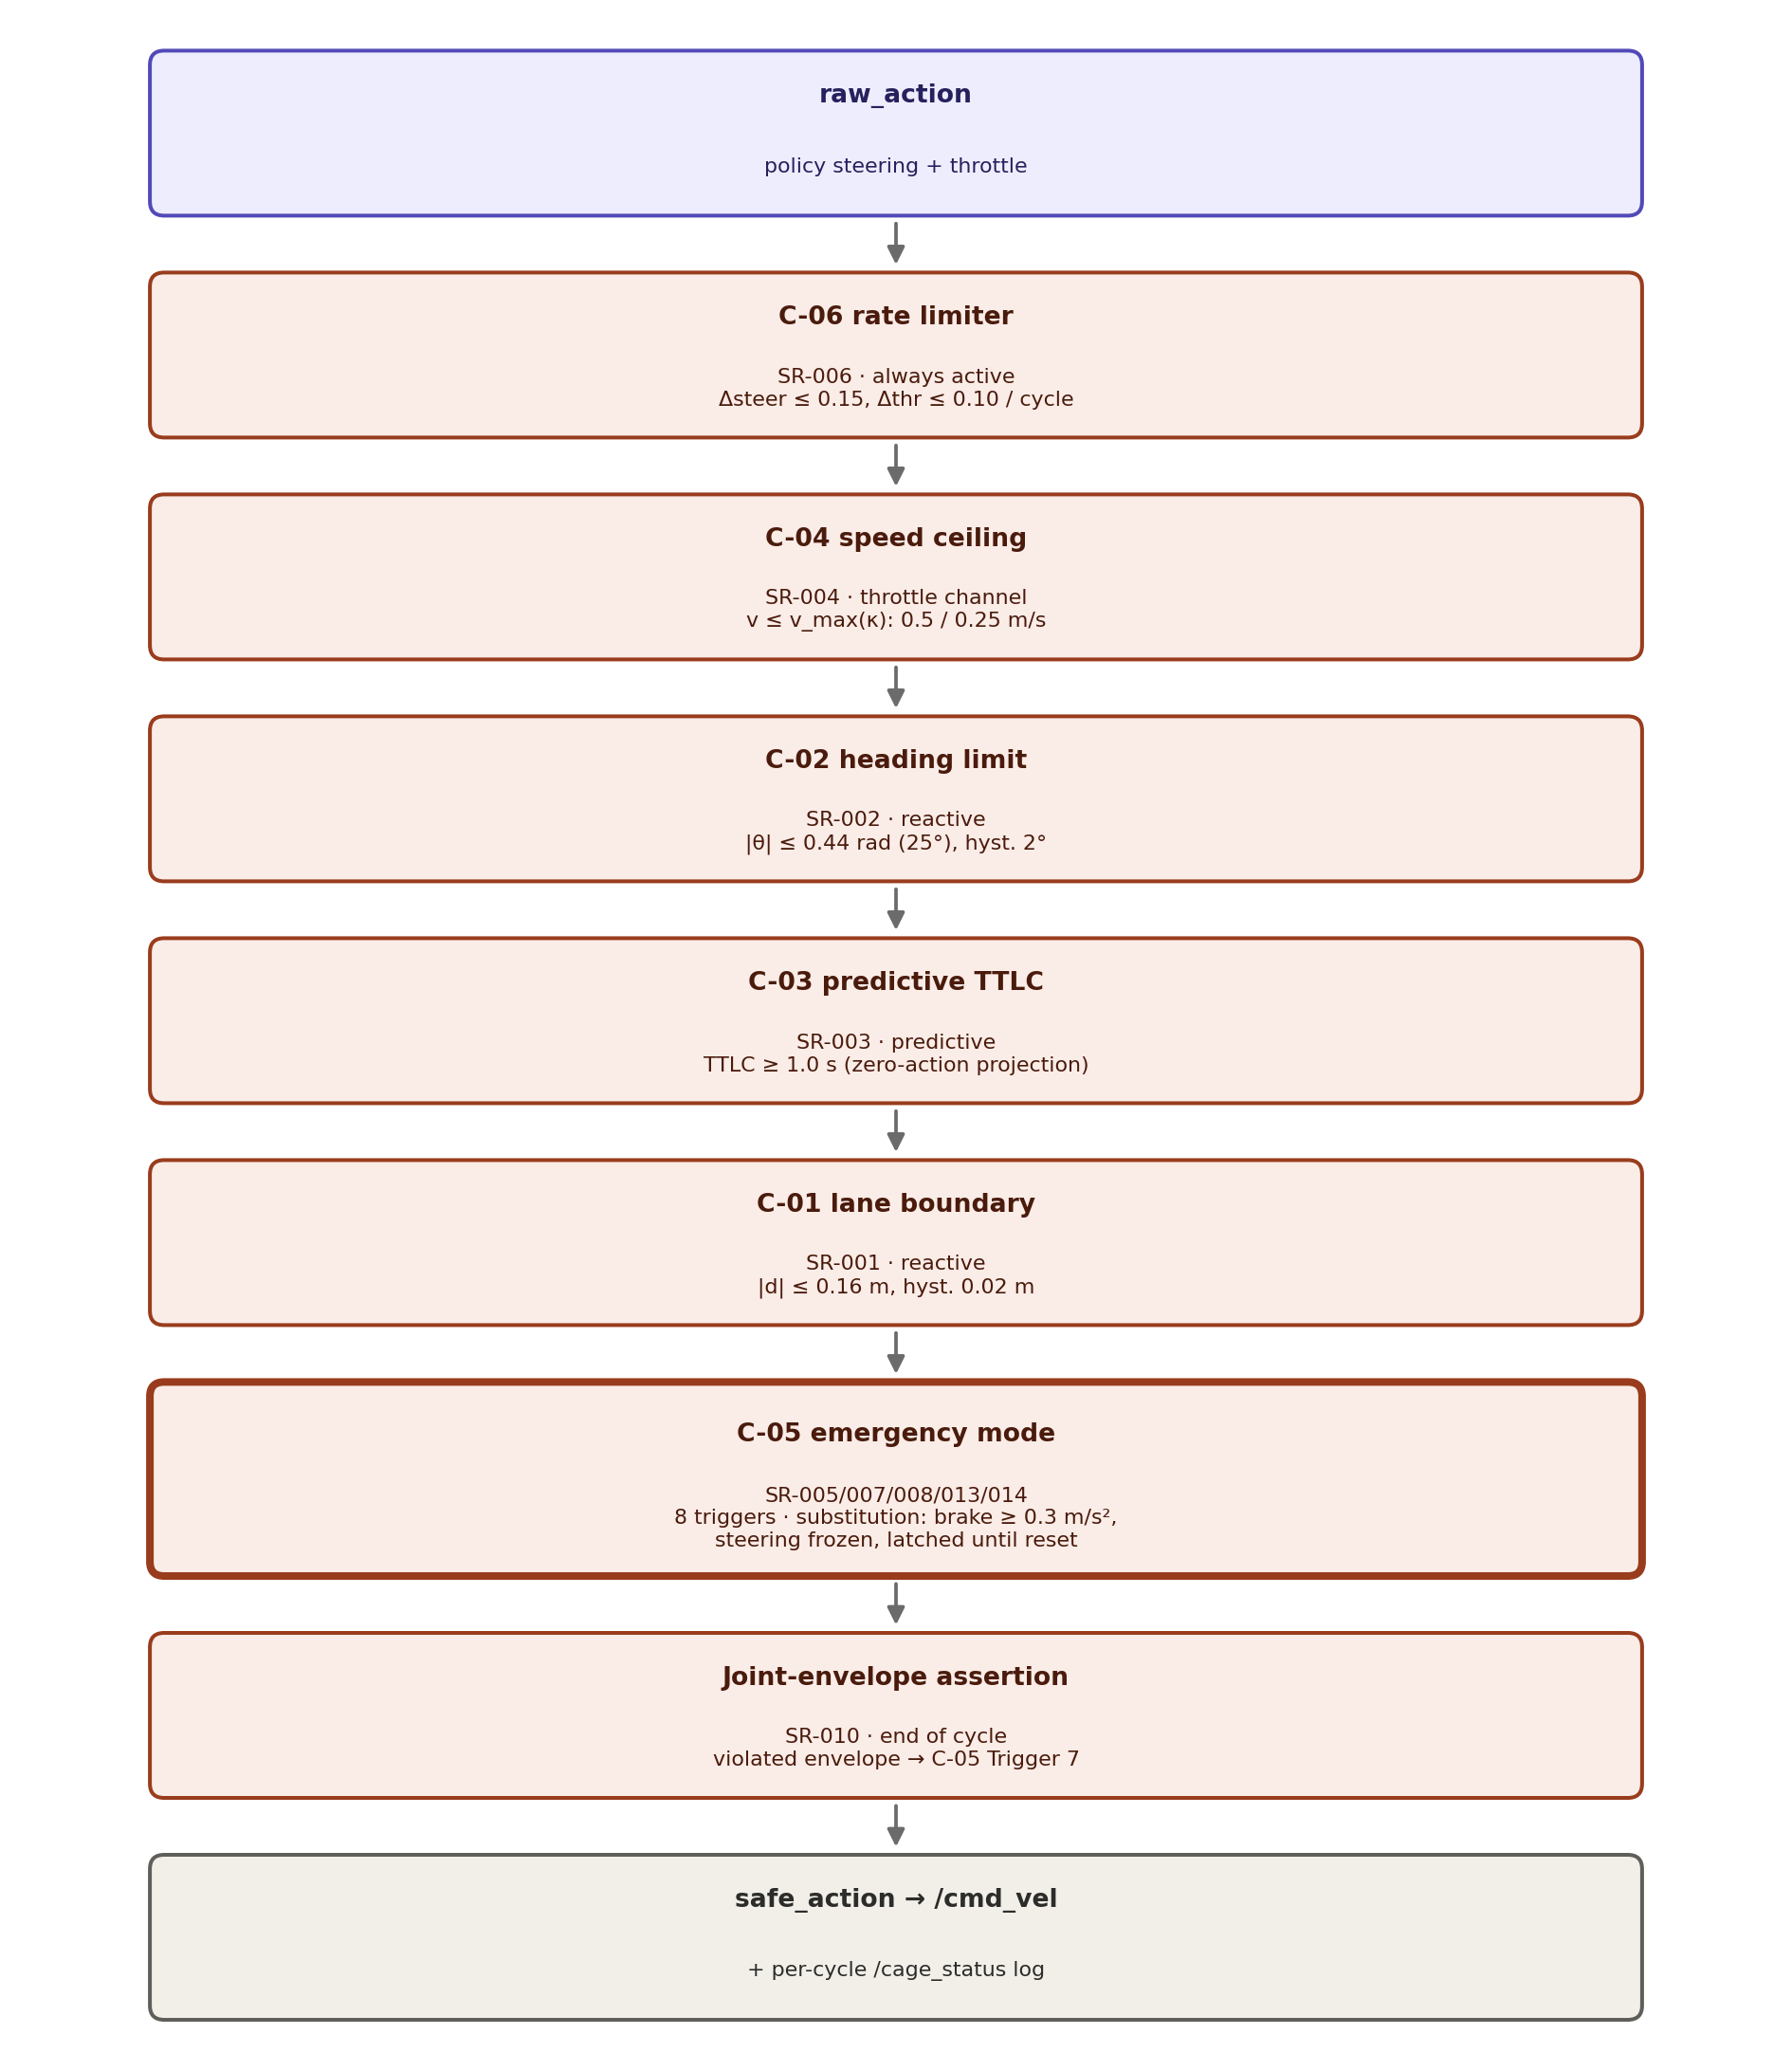
\includegraphics[width=0.80\widefigurewidth]{fig_5_1_cage_rule_chain.png}
  \caption[The rule chain in evaluation order.]{The six rules in their fixed evaluation order, one pass per cycle. Each rule takes the safe action of the previous rule as its raw action. \cagerule{06} first cleans the command into a feasible baseline. \cagerule{05} runs last, so its replacement action (steering frozen and braking) overrides every earlier correction. The joint-envelope check at the end of the cycle can still escalate to emergency.}\label{fig:5.1}
\end{figure*}

The six rules run in the fixed order shown in Figure~\ref{fig:5.1}, one pass per cycle. Each rule is described in the same format: requirement implemented, observed variable, activation logic, correction strategy and parameters. Using the same format makes it easier to compare and cross-check them. The full numerical values are in Appendix~\ref{app:E}.

\textbf{\cagerule{01} — Hard lateral limit.} It looks at the signed lateral offset. It activates with hysteresis above a threshold set below the requirement's limit, with a lower deactivation band and memory between cycles. The correction grows with the excess, points back towards the centre, and replaces the steering command. Throttle is not touched. If emergency mode is active, \cagerule{01} does nothing.

\textbf{\cagerule{02} — Heading error limit.} The same logic applied to the orientation error, with its own hysteresis band and gain. \cagerule{01} and \cagerule{02} can be active at the same time. In the chosen order \cagerule{02} runs first, so the final correction combines both and \cagerule{01} has the final say. This co-activation is exactly the case that hazard \hz{09} predicts, and Chapter~\ref{ch:08} measures it.

\textbf{\cagerule{03} — Predictive time-to-crossing limit.} It projects the lateral state over a short horizon with a simple kinematic model and estimates how long it will take to cross the lane boundary. If that time drops below the minimum, it applies a correction that grows with the urgency. Its benefit is that it adds margin before \cagerule{01} has to act. Its cost is that it depends on a projection model that gets less accurate as curvature increases.

\textbf{\cagerule{04} — Speed ceiling.} It limits the commanded speed with a ceiling that depends on the local curvature, interpolated between a value for straight track and a value for curves. It acts on the throttle. It is the only rule that never fires in the reference campaign. Chapter~\ref{ch:08} explains why, and the reason is a stated limitation of the operating point, not of the rule.

\textbf{\cagerule{05} — Emergency mode.} This is the most complex rule and the only one that can override all the others. Eight conditions can trigger it, in three groups. The first is an unrecoverable compound state: high heading error and offset that last over time. The second is an invalid state: an old observation, fields out of range, or lost messages. The third is perception health: the lane estimator reports that it cannot give a reliable estimate, or the estimate fails the plausibility check. The behaviour is deterministic: braking at a minimum rate with steering frozen until the vehicle stops. The last two groups are what make the system fall back to a safe stop instead of acting on bad perception, and they implement the camera-track requirements.

\textbf{\cagerule{06} — Rate limiter.} It limits how much the command can change between two cycles, for both steering and throttle. It runs first, on the raw command. Formally, it is the least critical rule, since it implements class B requirements on smoothness and variance. Chapter~\ref{ch:08} shows that this label greatly underestimates its real role in the final system.

\section{Parameters, versioning and modes}
\label{sec:5.6}

All thresholds are stored in a version-controlled parameter file, not in the code. This has three practical effects. First, every experimental run records the \emph{hash} of the file\sidenote{A cryptographic hash is a short fingerprint of a file. If one character of the file changes, the hash changes, so every run can be matched to its exact configuration.} together with the other reproducibility metadata, so each result is clearly linked to the exact configuration that produced it. Second, thresholds that still need physical calibration are marked in the file itself, so anyone reading it sees that they are provisional, instead of this being hidden somewhere in the documentation. Third, versioning follows a backward compatibility rule: when a new feature is added, its default values must keep it inactive for older configurations. This way an old campaign can be re-run without a newer feature changing its result.

The cage also has two operating modes\sidenote{Both modes run the same rules and log the same activations. The only difference is whether the corrected command reaches the vehicle, which is what makes monitoring a clean counterfactual.}, and the whole experimental design of this work is built on them. In enforcement mode, the corrections are applied to the command sent to the vehicle. In monitoring mode, the cage checks exactly the same rules and logs exactly the same activations, but does not change the command, so the policy drives alone. Comparing both modes on the same scenario and the same seed is how Chapter~\ref{ch:08} measures what the cage contributes. The value of this method is that it gives a clean counterfactual: it does not compare different systems, but the same system with and without the envelope active.

\section{ROS2 architecture}
\label{sec:5.7}

\subsection{Nodes}
\label{sec:5.7.1}

The system is split into the nodes shown in Figure~\ref{fig:5.2}. Each node has one job, and they communicate through explicit topics. The data flow is linear and easy to audit. Perception produces the state. The policy reads the state and produces a raw command. The cage reads the raw command and the state and produces a safe command and a cage status record. Vehicle control turns the safe command into actuation setpoints. The logging node writes the cage status to disk.

\begin{figure*}[htbp]
  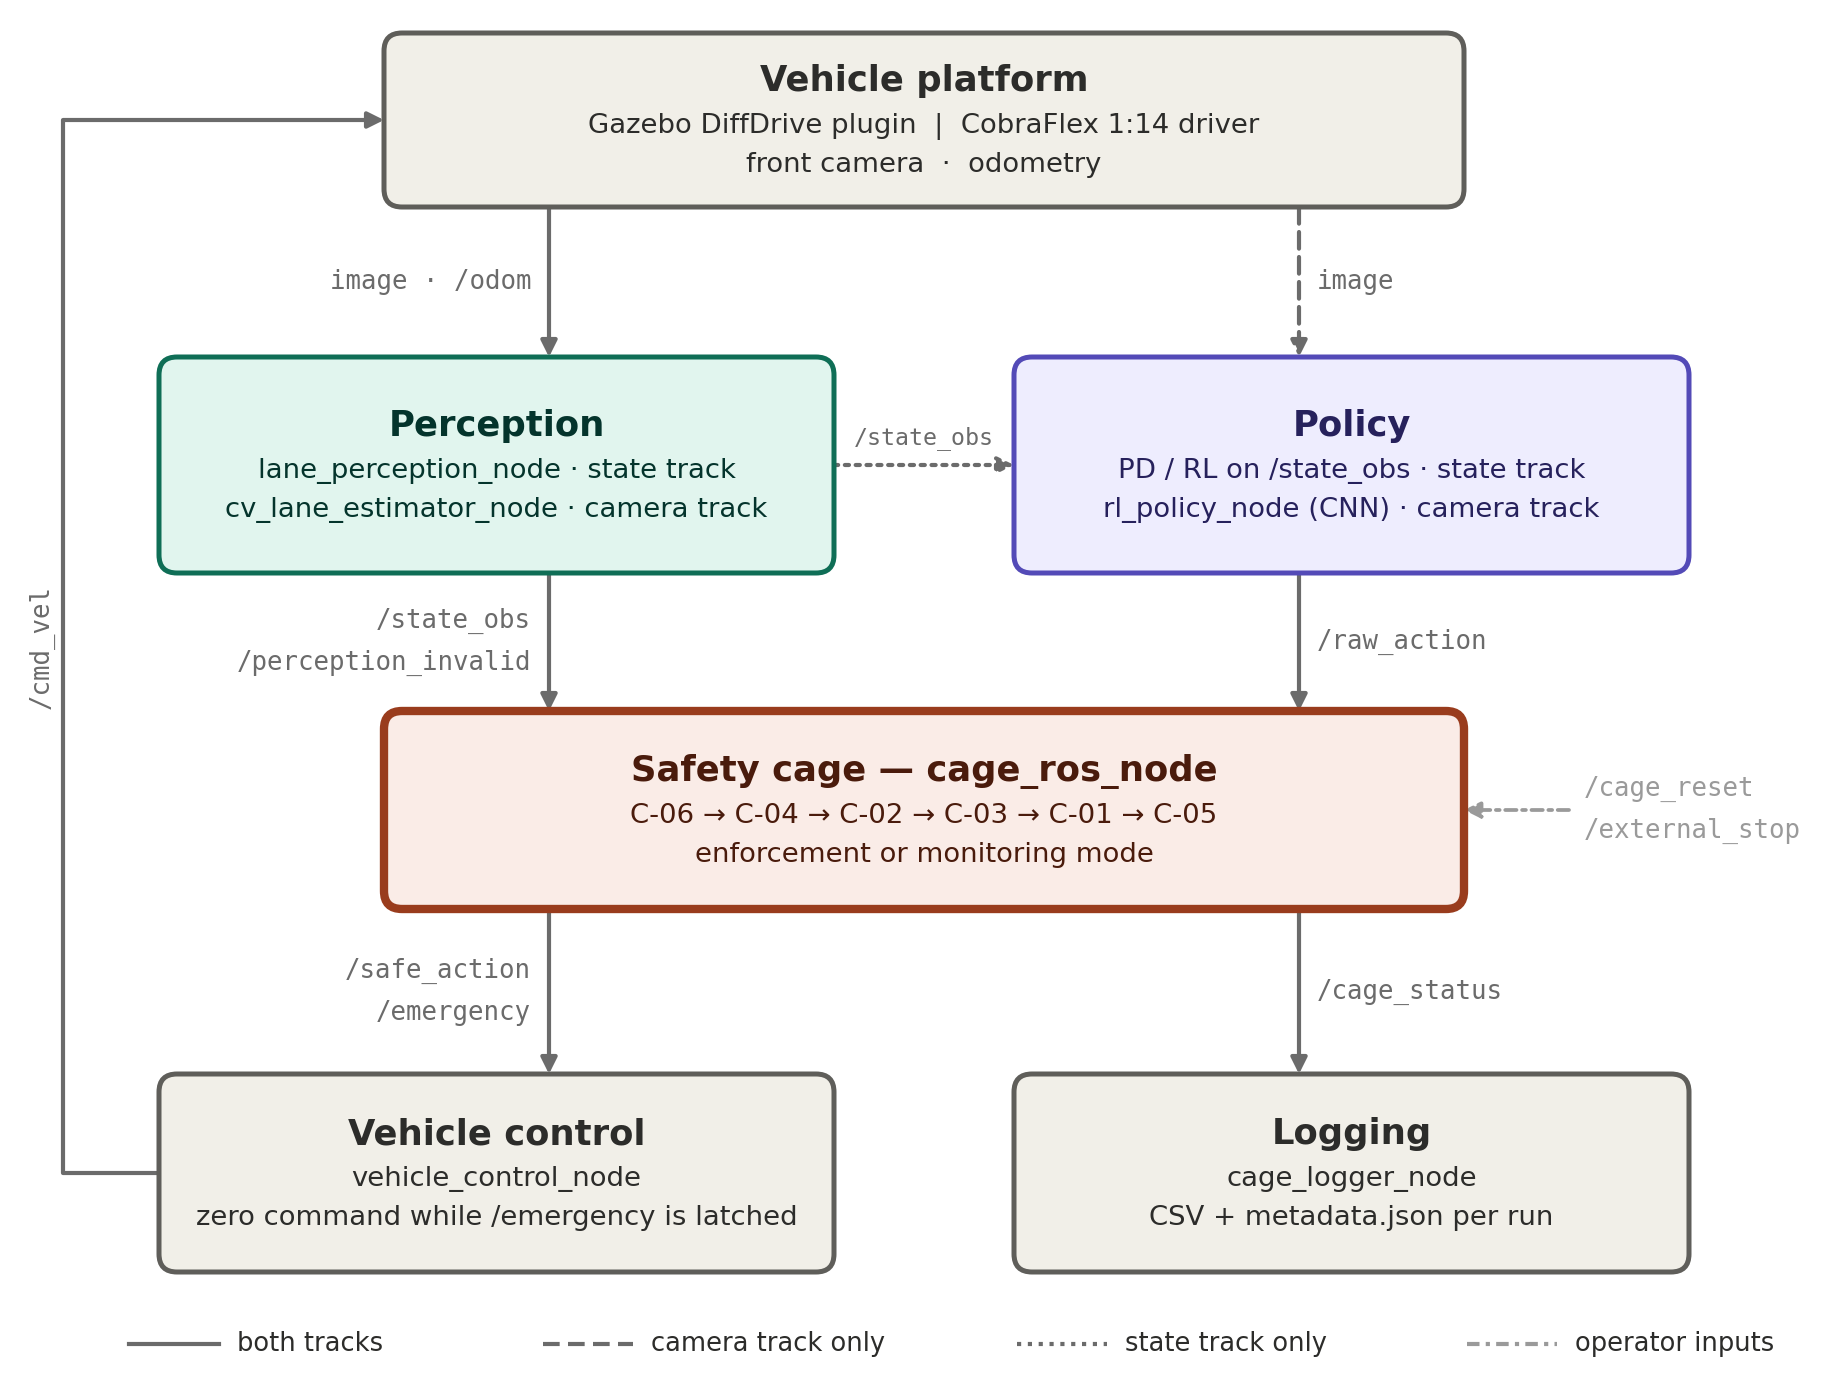
\includegraphics[width=0.83\widefigurewidth]{fig_5_2_node_chain.png}
  \caption[Node graph of the system.]{Node graph of the system: perception, policy, cage, vehicle control and logging, with the topics that connect them. In the state track the policy reads the state published by perception. In the camera track it reads the image directly, and the cage gets its state from the CV lane estimator (\S\ref{sec:5.7.2}). The only connection to the platform, \texttt{/cmd\_vel}, comes from vehicle control, which only receives input from the cage: the policy's command never reaches the actuator without going through it.}\label{fig:5.2}
\end{figure*}

The important architectural property is that the policy's command cannot reach the actuator without passing through the cage. This is not a coding convention. It is a property of the graph's topology that can be checked by looking at the connections, and it means there is no path for an unfiltered command to reach the vehicle.

\subsection{Camera track architecture}
\label{sec:5.7.2}

The camera track keeps the same topology, with two important differences. The policy gets the image instead of the state vector. And the cage gets its state from its own lane estimator, a classical computer vision pipeline that processes the same image with a deterministic algorithm that does not depend on the network.

This is the most delicate design point of the work, and its trade-off needs to be stated clearly. The benefit is that the safety envelope does not inherit the failure modes of the network. It works on a state produced by an algorithm that can be audited, read line by line and checked against a reference. The cost is a common cause\sidenote{A common cause is one fault that defeats two protections that are meant to be independent. Here it is a degraded image that blinds the policy and the cage estimator at the same time.}: both use the same image, so a bad enough degradation of the visual channel blinds both at once. The design does not hide this. It reduces the risk with the \cagerule{05} health and plausibility triggers, which fall back to a controlled stop when the estimator cannot give a reliable estimate. It also records it as a residual risk, with its own hazard (\hz{12}) for the case where the estimate is wrong \emph{but plausible}. No internal consistency check can catch that case.

\section{Traceability and automatic checks}
\label{sec:5.8}

Now that the rules are specified, the matrix covers its second part: the links between requirements and rules. The checker verifies three conditions automatically. Every rule implements at least one requirement. Every requirement is implemented by a rule, or explicitly states another type of implementation. And every rule is tested by at least one scenario. Any violation blocks the review gate.

The effect this has on design is worth pointing out, because Chapter~\ref{ch:11} evaluates it. The constraint forces the implementation path to be chosen when the requirement is written, not later. The visible result is a set of more practical requirements, and a set of rules with no orphan functionality: every rule in the cage answers a requirement that can be traced back to a registered hazard.

With the specification defined, Chapter~\ref{ch:06} covers its implementation and verification.

% Converted from manuscript/draft_v5_en/body/06_implementation.md
% Chapter 6 — Implementation and Verification

\chapter{Implementation and Verification}
\label{ch:06}

\section{Purpose of the chapter}
\label{sec:6.1}

This chapter occupies the implementation level (L5) and its symmetric level of classical verification (L4a'). It documents how the simulation environment, the system nodes and the cage specified in \Cref{ch:05} are materialised, and how that cage is verified with the technique that is still applicable to a deterministic component: the unit test.

The intention is not engineering exhaustiveness but to document \textbf{the non-trivial decisions} and the evidence that the chain works before the learned component is introduced.\sidenote{The complete inventory of modules, scripts and tests lives as a version-controlled living document.}

\section{Simulation environment and vehicle modelling}
\label{sec:6.2}

The environment is built on a ROS2 distribution and a Gazebo version with long-term support, chosen for coherence with the rest of the chain and for the availability of the native bridge between them. The simulated world reproduces a delimited track with white side markings and a dashed central separator, on a flat surface and with controlled lighting; its geometric parameters are exactly those declared by the operational domain, so that any claim about the domain can be checked against the world file.

The vehicle is modelled by approximating the dynamics of the physical scale vehicle. One important and frequently overlooked clarification: the real platform is \textbf{differential drive}, with four fixed wheels and no steering angle, and not of the Ackermann type; the simulation model uses a differential drive controller and is faithful in that sense. The practical consequence is that \enquote{steering} in this whole work means a normalised angular velocity setpoint, not a wheel angle, and that the manoeuvrability envelope of the simulator and that of the platform share the same structure.

\section{Implementation of the nodes}
\label{sec:6.3}

All nodes follow a common pattern: externalised and declared parameters, explicit subscription and publication, a fixed-frequency loop governed by a timer, and structured logging. The uniformity is not cosmetic: it makes latency and temporal behaviour attributable to a specific node when something deviates.

\paragraph{Perception node} On the state track it projects the pose onto the centre line in order to produce the state vector. On the camera track this role is played by the vision estimator of the cage itself, described below.

\paragraph{Policy node} It loads the trained model, consumes the observation and publishes the raw command. It is deliberately thin: all the learning logic lives in the training environment, and in operation the node is an evaluator of the policy.

\paragraph{Cage node} This is the central component. It is implemented as a \textbf{pure Python library with no ROS2 dependency}, wrapped by a thin node that connects it to the topics. This separation has a methodological consequence that deserves to be highlighted: the cage can be \textbf{tested completely without starting the simulator or the middleware}, with a deterministic suite that runs in less than one second. The verifiability that \Cref{ch:05} claimed in the abstract becomes operational in this way.

\paragraph{Vehicle control node} It translates the safe command into actuation setpoints, applying the final physical saturation.

\paragraph{Logging node} It persists the complete cage status per cycle --- raw command, safe command, active rules, mode, observed state --- to a structured file. It is the instrument of the runtime monitoring level: without it, adaptation A3 would have no evidence.

\section{A classical controller as a chain validator}
\label{sec:6.4}

Before introducing the learned component, a \textbf{proportional-derivative controller} over the lateral and heading error is implemented. Its function in the thesis is not to compete with the policy but to do three different things: to validate that the complete chain works end to end with a controller whose behaviour is entirely predictable; to offer a \textbf{performance reference} against which the learning results can be interpreted; and to allow the cage thresholds to be calibrated with a driver whose behaviour does not change between runs.

Its limitations are declared: it does not anticipate curvature, it degrades on tight curves and its gains were tuned empirically on one concrete geometry. It is not a competitive baseline, it is an instrument.

\section{Verification strategy and results}
\label{sec:6.5}

Verification is organised on three levels. The \textbf{unit tests per rule} cover, for each of the six rules, at least the activation above the threshold, the non-activation below it, the behaviour inside the hysteresis band in both directions, and the saturation. The \textbf{transversal property tests} verify invariants that no rule owns on its own: that the evaluation order is the declared one; that the emergency mode dominates any previous correction; that the output command is always inside the physical range independently of how many rules intervened; and that a parameter configuration of an earlier version still produces the earlier behaviour. The \textbf{integration tests} exercise the complete chain with synthetic states, checking that the command arrives filtered and that the log contains what it should contain.

The suite grows with the system and is run as a condition of each review. Its value is not in the number of cases but in one property: \textbf{every cage rule has tests that fail if its behaviour changes}, which turns any threshold modification into a visible change and not into a silent drift.

\section{Chain validation and preliminary metrics}
\label{sec:6.6}

The integrated demonstration runs the complete chain in simulation with the classical controller in command. Three preliminary metrics are reported, \textbf{not as an experimental result but as evidence that the chain works}.\sidenote{The characterisation belongs to \Cref{ch:08}.}

The \textbf{cage cycle latency}, measured over 845 s of continuous operation, gives a median and a 95th percentile of 50.0 ms, with a maximum of 62.0 ms attributable to a single cycle and to the non-deterministic scheduler of the operating system. Median and 95th percentile fit inside the budget of the control cycle.

The \textbf{intervention rate} during nominal operation is 0.047\,\% of the cycles,\sidenote{8 out of 16,910.} all of them attributed to the heading rule or to the rate limiter, with no activation of the lateral limit, of the predictive rule or of the emergency. The reading goes in two directions and both matter: the classical controller is well calibrated for the nominal scenario, \textbf{and} the cage thresholds are not artificially restrictive. A cage that intervened constantly under nominal conditions would not be measuring safety, it would be measuring its own misadjustment.

The \textbf{completion rate} under nominal conditions is 9.91 laps in 845 s with no emergency cycle at all. With a single run it is not possible to speak of characterisation; what the figure establishes is that the chain sustains prolonged operation without degradation.

\section{Specialisation for the camera track}
\label{sec:6.7}

The reference system \textbf{does not add nodes: it specialises the environment}. The same training environment serves both tracks, and the camera branch is activated with a configuration switch. Four technical decisions deserve to be recorded.

\paragraph{Shared camera chain and common-cause guarantee} The native image arrives through the bridge between simulator and middleware and goes through a single chain per cycle. The visual degradation injector of the scenario is applied \textbf{before} the branching, so that the same degraded image feeds both the cage estimator, at native resolution, and the reduction to $84\times84$ in grey scale that the policy consumes. Applying the degradation only once, before the branching, is what guarantees that \textbf{policy and cage see the same world, also when that world is degraded}. One implementation finding has a direct consequence for the experimental budget: camera rendering is tied to real time, so the simulation clock runs at factor one on this track, as opposed to the accelerated execution of the state track.

\paragraph{Lane estimator of the cage} It is a classical and deterministic vision chain that reconstructs the lateral offset and the heading error for the six rules.\sidenote{Thresholding, line extraction and lane geometry.} Its validation is \textbf{its own and prior to the verdict}: against the ground truth oracle of the simulator it reaches complete detection with an offset bias below 32 mm under the glare levels that the scenario campaign later uses. When its health supervisor declares perception invalid, the emergency mode executes the controlled stop in open loop: the mechanism that \Cref{ch:08} measures as the value of the cage under degradation.

\paragraph{Validation circuit} The reference track is validated on a winding and self-approaching circuit of 19.22 m perimeter --- 2.2 times the oval of the state track --- and on its visual stress variants. The self-approaching layout forced a change in the containment logic: the perpendicular off-road criterion collapses when two sections of the layout are closer than one road width, so departure is judged by \textbf{global distance to the road axis}, keeping the earlier behaviour intact for the state track. It is an instructive example of how a change of geometry silently invalidates a metric that looked neutral.

\paragraph{Visual randomization during training} The training applies random visual degradations inside the envelope of the corresponding hazard, as a robustness mitigation. In evaluation the randomization is \textbf{switched off}, and the only visual stressor is the one declared by the scenario, so that every run is attributable to its perturbation. Mixing the two would produce results that could not be attributed.

\section{Synthesis}
\label{sec:6.8}

At the close of this chapter the system exists: the chain works end to end, the cage is implemented and verified with the classical technique that its deterministic nature admits, and the logging produces the evidence that the upper levels of the right branch will consume. What is missing is the component that the framework exists to accommodate. \Cref{ch:07} addresses its process specification --- the second half of adaptation A1 --- and its training.

% GENERATED by md2tex.py from ../draft_v5_en/body/07_training.md -- do not edit by hand.
% Change the Markdown and run `python md2tex.py`; edits here are overwritten.

\chapter{Training specification and execution}
\label{ch:07}

\section{Purpose of the chapter}
\label{sec:7.1}

This chapter covers the second half of adaptation A1: the Training Specification. It is a meta-specification, not a specification of behaviour. It does not say what the policy will do in a given state, because it cannot. Instead it fixes the process that produces the policy: observation and action spaces, reward function, termination criteria, the role of the cage during training, hyperparameters, seeds and how checkpoints are kept. Someone with this document and the code can repeat the process, but cannot predict the result. That difference is the point of the adaptation.

The full hyperparameter table and the comparison between algorithms, with its eight configurations and the checkpoints that were evaluated, are in Appendix~\ref{app:H}.

\section{Process specification}
\label{sec:7.2}

\subsection{Observation and action}
\label{sec:7.2.1}

The observation of the reference system is the front camera image, reduced to 84$\times$84 in greyscale and stacked over four consecutive frames\sidenote{With one frame the network sees a position. With four it also sees motion, so it can tell whether the car is moving towards the edge or away from it.} so that the policy gets information about motion. The stacking is not a small implementation detail. Without it, the policy cannot tell a static situation from a moving one, and the heading error becomes partly unobservable. The network is a standard convolutional network of the kind used for control from pixels.

The action space is a configuration choice, not something fixed for the whole work. How it changed between its two values is one of the main threads of this chapter. For most of the project the action was one-dimensional: steering only, with a fixed forward speed. This reduces the problem to lateral control and keeps a clear line between what the reward guides and what the cage guarantees. The final reference configuration is two-dimensional, with steering and throttle, a speed ceiling of 0.22 m/s and a dead band in the throttle command\sidenote{A dead band ignores very small throttle commands, so that noise around zero does not make the vehicle creep or jerk.}. The difference matters. In 1-D the cage's speed rules can never act, because the policy does not decide the speed. Only when the policy controls speed can those rules intervene.

\subsection{Reward function}
\label{sec:7.2.2}

The reward has four terms. Progress along the circuit is the task signal. A penalty on lateral error keeps the vehicle centred in the lane. A penalty on heading error keeps it aligned with the track. And a penalty on changes in the command discourages jerky driving. The two-dimensional configuration adds a fifth term, to stop the policy from simply stopping. Without it, a policy that controls the throttle finds that parking avoids all the penalties. This is a textbook case of the reward exploitation hazard that the hazard register had predicted.

The link between reward and safety is one of the most important design decisions of this work, so it needs to be stated clearly: the reward has no safety terms. It does not penalise cage activations, and it does not reward staying away from the limits. The reason is a split of responsibilities, where the reward guides and the cage guarantees. This has a useful side effect for the experiments. Since the policy was not trained to satisfy the cage, how often the cage intervenes is a clean measure of how good the learned driving is.

\subsection{The cage during training}
\label{sec:7.2.3}

The cage is active in the training loop and filters the command before it reaches the simulated vehicle. The advantages are clear: episodes are not wasted on crashes, and the agent learns the dynamics of the system as it will be deployed. There is also a cost, which this work did not fully expect and which Chapter~\ref{ch:08} reports as a finding. If the cage shapes the command during training, the policy learns against a system that already contains the cage, so what is optimised is the pair and not the policy alone.

\subsection{Reproducibility}
\label{sec:7.2.4}

Every training run records the seed, the configuration version, the \emph{hash} of the cage parameter file, the code revision and a timestamp. Checkpoints are saved at fixed intervals\sidenote{A checkpoint is a saved copy of the network weights at a given training step. Any checkpoint can later be loaded and evaluated on its own.}, and each one has a cryptographic identifier that links it to its configuration. If an evaluation tries to load a checkpoint whose configuration does not match, it fails with an error instead of quietly producing an invalid result. The mechanism is simple, and it prevented at least one serious mix-up during the project.

The text uses descriptive names for trainings, checkpoints and campaigns, while figures and appendices use the short labels from the repository. Table~\ref{tab:7.1} connects the two.

% layout: table*, fixed, \small, 164 of 165 mm
\begin{table*}[htbp]
\caption[Names of trainings, checkpoints and campaigns.]{Names of trainings, checkpoints and campaigns. Conventions: \texttt{k} after a number counts thousands of training steps (\texttt{550k} = 550,000; \texttt{@297k} = at 297,000 steps); \texttt{1-D} and \texttt{2-D} give the size of the action (steering; steering and throttle); \texttt{cap} is the speed ceiling of the action; \texttt{complex\_b} is the winding circuit (perimeter 19.22 m) and \texttt{oval} the oval one (R = 0.8 m); \texttt{newcam} in a run name marks runs made after the switch to the dedicated lane camera.}\label{tab:7.1}
\small\setlength{\tabcolsep}{4pt}
\begin{tabular}{@{}>{\RaggedRight\arraybackslash}p{28.4mm}>{\RaggedRight\arraybackslash}p{23.6mm}>{\RaggedRight\arraybackslash}p{106.0mm}@{}}
  \toprule
  \tabhead{Label in figures and appendices} & \tabhead{Name in the text} & \tabhead{What it is} \\
  \midrule
  \texttt{F-track} & State track (control arm) & The policy observes a state vector projected from the true pose, on the oval circuit; it isolates the effect of the cage (\S\ref{sec:1.6.3}). Campaign: \texttt{campaign}. \\
  \addlinespace[2pt]
  \texttt{track E}, \texttt{E-track} & Camera track & The policy observes the front-camera image; the reference system of the thesis. \\
  \addlinespace[2pt]
  \texttt{E-main}, \texttt{1-D PPO}, \texttt{297k} & One-dimensional camera policy & PPO, steering only at a fixed 0.20 m/s on \texttt{complex\_b}; checkpoint kept at the reward peak, 297,000 steps (\S\ref{sec:7.3}). Run: \texttt{ppo\_\allowbreak{}newcam\_\allowbreak{}complex\_\allowbreak{}b\_\allowbreak{}2024\_\allowbreak{}1M}. \\
  \addlinespace[2pt]
  \texttt{seed 2024}, \texttt{42}, \texttt{23}, \texttt{666}, \texttt{123} & The five seeds & Copies of that training that differ only in the seed (\S\ref{sec:7.4}). Runs: \texttt{ppo\_\allowbreak{}newcam\_\allowbreak{}complex\_\allowbreak{}b\_\allowbreak{}<seed>}. \\
  \addlinespace[2pt]
  \texttt{GE4-V2}, \texttt{campaign\_e\_v2} & Campaign of the one-dimensional policy & Second version of the scenario campaign of gate G4, run on \texttt{E-main}: 1,970 runs, kept frozen as the gate record. \\
  \addlinespace[2pt]
  \texttt{margin022}, \texttt{2-D SAC} & First two-dimensional campaign & SAC, steering and throttle, speed cap 0.22 m/s, which is 0.03 m/s below the 0.25 m/s curve ceiling of \cagerule{04} (hence the name); checkpoint at 75,000 steps; 1,970 runs (\S\ref{sec:7.5.1}). Run: \texttt{sac\_\allowbreak{}gz2d\_\allowbreak{}entfix\_\allowbreak{}margin022\_\allowbreak{}2024\_\allowbreak{}75k}; campaign: \texttt{campaign\_\allowbreak{}2d\_\allowbreak{}margin022}. \\
  \addlinespace[2pt]
  \texttt{2-D PPO 550k}, \texttt{cap 0.22} & Reference policy and reference campaign & PPO, steering and throttle, speed cap 0.22 m/s; checkpoint at 550,000 steps chosen by closed-loop driving (\S\ref{sec:7.5.2}); its 1,890-run campaign gives the verdict (Chapter~\ref{ch:08}). Run: \texttt{ppo\_\allowbreak{}gz2d\_\allowbreak{}cap022\_\allowbreak{}1M\_\allowbreak{}2024}; campaign: \texttt{campaign\_\allowbreak{}2d\_\allowbreak{}ppo550k}. \\
  \addlinespace[2pt]
  \texttt{sim-to-real v2}, \texttt{1650k} & Policy retrained for transfer & Two-dimensional PPO retrained with per-episode mirroring and randomisation of photometry and camera geometry, 2.5 million steps; checkpoint at 1,650,000 steps deployed on the vehicle (\S\ref{sec:9.3.4}). Its \texttt{v2} has nothing to do with \texttt{GE4-V2}. Run: \texttt{ppo\_\allowbreak{}gz2d\_\allowbreak{}sim2real\_\allowbreak{}v2\_\allowbreak{}2024}. \\
  \bottomrule
\end{tabular}
\end{table*}

\section{Results of the one-dimensional camera policy}
\label{sec:7.3}

The first camera policy that drives well is trained on the winding circuit with a one-dimensional action. Its mean episode reward rises to a peak of $\approx$ 823 at around 297,000 steps, stays high for about 150,000 more steps, and then drops. The cause matters. The critic loss stays very small during the whole run, so the problem is not an unstable value function. Instead, exploration shrinks once the policy's standard deviation is annealed too far\sidenote{PPO samples its actions from a distribution whose width, the standard deviation, is reduced during training. When the width becomes too small the policy stops trying new actions.}. This is why the checkpoint kept is the one at the peak and not the one at the end.

\begin{figure*}[htbp]
  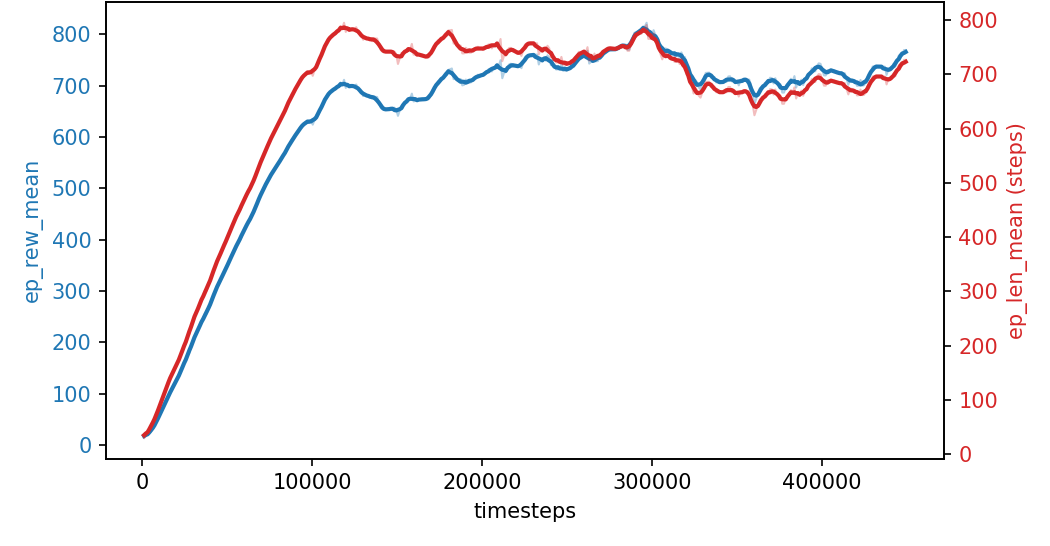
\includegraphics[width=0.87\widefigurewidth]{fig_7_1_convergence_newcam_notitle.png}
  \caption[Convergence of the one-dimensional camera training.]{Convergence of the one-dimensional camera policy (\texttt{E-main}, Table~\ref{tab:7.1}): reward and mean episode length against steps. Peak $\approx$ 823 and a high plateau. The later collapse in exploration led to stopping the run by hand and keeping the checkpoint at the peak.}\label{fig:7.1}
\end{figure*}

\begin{figure*}[htbp]
  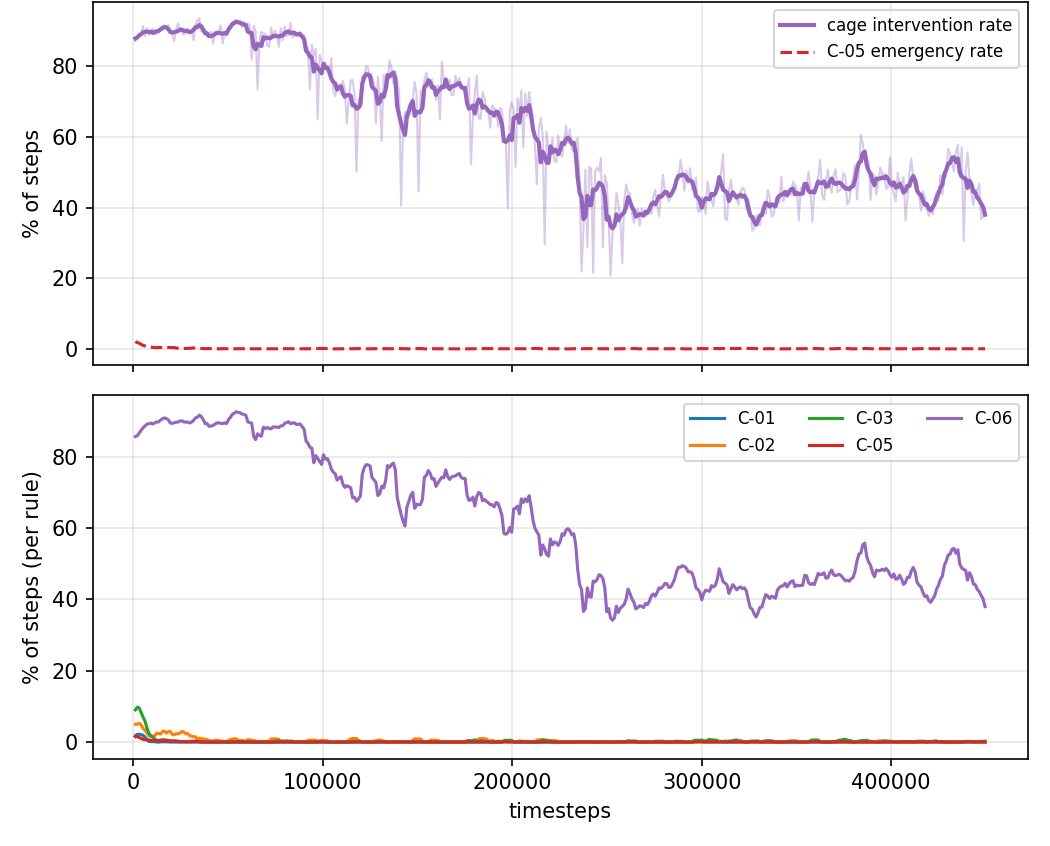
\includegraphics[width=0.87\widefigurewidth]{fig_7_2_intervention_newcam_notitle.png}
  \caption[Cage activity during training.]{Cage activity during the one-dimensional training. Top: the total intervention rate falls from $\sim$87\,\% to $\sim$40\,\%, while the emergency rate is zero from the start. Bottom: the per-rule breakdown shows what that rate is made of. It is the rate limiter. The safety rules \cagerule{01}, \cagerule{02}, \cagerule{03} and \cagerule{05} drop to zero in the first steps and stay there.}\label{fig:7.2}
\end{figure*}

A second result of this training, shown in Figure~\ref{fig:7.2}, is that policy and cage adapt to each other. The intervention rate falls from $\sim$87\,\% at the start to $\sim$40\,\%, mostly from the rate limiter, while the safety rules drop to zero. The policy therefore learns to respect the safety constraints and does not go near the edge, but its steering is still jerky and the limiter keeps smoothing it.

Table~\ref{tab:7.2} gives the deterministic nominal evaluation against a classical controller on the same circuit. It is the result that justifies the cost of the learned component:

% layout: table*, natural, \small, 113 of 165 mm
\begin{table*}[htbp]
\caption{Nominal evaluation: camera policy against the classical baseline on the same circuit.}\label{tab:7.2}
\small\setlength{\tabcolsep}{4pt}
\begin{tabular}{@{}lll@{}}
  \toprule
  \tabhead{Metric (nominal scenario)} & \tabhead{Classical baseline} & \tabhead{\textbf{1-D camera RL}} \\
  \midrule
  Laps completed & 4.85 & 4.88 \\
  Mean lateral error & 17.2 mm & 10.9 mm \\
  Maximum lateral error & 57.3 mm & 48.2 mm \\
  Emergency stops & 0 & 0 \\
  Cage intervention & 0\,\% & 43.5\,\% (limiter only) \\
  \bottomrule
\end{tabular}
\end{table*}

The agent is more precise than the classical baseline, with 37\,\% less mean lateral error over the same distance and zero emergencies. This is the opposite of the result on the oval, where the classical controller was more precise. On a winding layout the look-ahead point of the classical method becomes less reliable, while the network keeps its line.

Two further observations come with this result. First, the cage stays latent inside the domain in both modes: there are zero emergencies and no safety rule activations, only the rate limiter, and enforcement and monitoring give almost the same laps and errors. Second, the cost of the learned agent is smoothness, not safety. It triggers the limiter in 43\,\% of the steps, against 0\,\% for the classical controller, and this intervention is harmless, because it absorbs the jerky steering without hurting precision.

\section{Variation between seeds}
\label{sec:7.4}

A result from a single seed says nothing about a stochastic procedure. Repeating the training with five seeds, shown in Figure~\ref{fig:7.3}, gives the most uncomfortable and probably the most useful finding of the chapter: the training curve does not tell how the policy behaves. Three of the five seeds respect the constraints, so the cage stays latent. The other two rely heavily on the cage, with hundreds of safety interventions. This difference cannot be predicted from the training reward, because seeds with almost identical curves end up on different sides.

\begin{figure*}[htbp]
  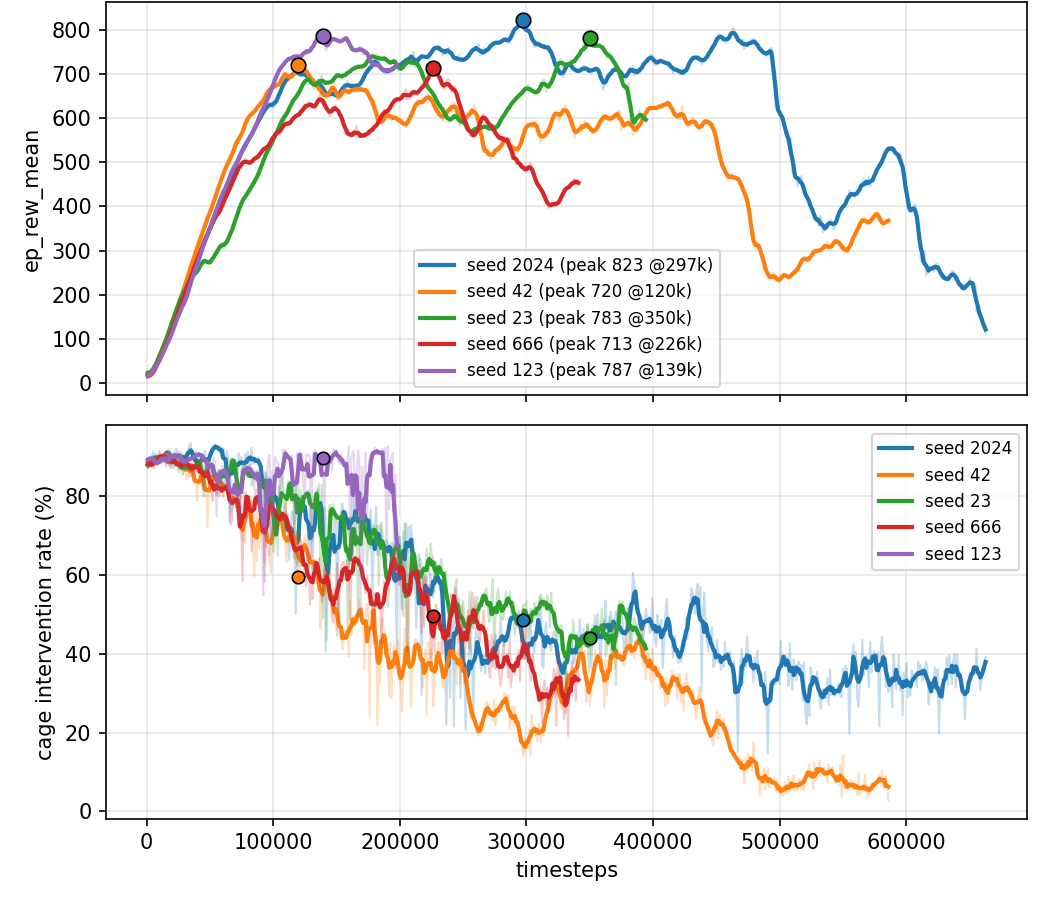
\includegraphics[width=0.87\widefigurewidth]{fig_7_8_multiseed_newcam_notitle.png}
  \caption[Comparison across five seeds.]{Five seeds of the same procedure (Table~\ref{tab:7.1}; \texttt{@297k} marks the step of each peak). Top: the reward, with similar curves and peaks from 713 to 823, none clearly better than the others. Bottom: the cage intervention rate for the same runs, which does separate them. The information that tells the behaviours apart is in the bottom panel, which is exactly the panel a selection by reward ignores.}\label{fig:7.3}
\end{figure*}

The consequence for the method is direct and applies to the rest of the work: the policy cannot be chosen by reward. It has to be chosen by closed-loop evaluation on scenarios\sidenote{Closed loop: the policy drives, its actions change what the camera sees next, and the outcome is measured. The training reward is collected with exploration and visual randomisation switched on.}, with the cage intervention rate as a main criterion. This is a concrete example of what the framework is supposed to produce: an acceptance criterion that no training metric would have given.

\section{The reference policy: two-dimensional action}
\label{sec:7.5}

\subsection{Motivation and choice of algorithm}
\label{sec:7.5.1}

The first attempt at a full campaign with a two-dimensional action used a weak policy. It was weak in two ways: the algorithm was used outside the range where it works well, and the training was short. In addition, the checkpoint came after the peak instead of at the peak. The result raised a clear question: were the failures caused by the two-dimensional action or by that particular policy? To answer it, a proper two-dimensional policy was trained, with two changes, both measured.

\textbf{Algorithm.} PPO, the on-policy method, reaches a mean reward of 1755 at around 472,000 steps (Figure~\ref{fig:7.4}), with a high and stable plateau. SAC, the off-policy method, never goes above $\sim$200 and never learns to drive the circuit. This is the experimental comparison announced in \S\ref{sec:2.2}, and it settles the algorithm for the rest of the work.

\textbf{Speed ceiling.} A comparison that changes only this variable shows that at 0.5 m/s the policy peaks at 654 and drives badly, overshooting the tight curves. At 0.22 m/s it reaches 1421 and takes them cleanly.

One warning about these numbers. Reward cannot be compared directly between action spaces, because the maximum episode reward doubles when moving to two dimensions. The factor of about 2 compared with the one-dimensional policy comes mostly from surviving longer and from a longer horizon, not from driving twice as well.

\begin{figure*}[htbp]
  
\includegraphics[width=0.96\widefigurewidth]{auto/fig_7_4_ppo2d_training_curve.png}
  \caption[Training curve of the two-dimensional reference policy.]{Training reward of the two-dimensional reference policy (\texttt{2-D PPO}) compared with the one-dimensional policy (\texttt{E-main}) and with the off-policy version (\texttt{margin022}); labels in Table~\ref{tab:7.1}. Peak 1755 and a high stable plateau, against the collapse after the peak of the first one and the $\sim$200 ceiling of the second. Marked: the three candidate checkpoints evaluated in closed loop, including the selected one, and the checkpoint kept from each of the other two runs.}\label{fig:7.4}
\end{figure*}

\subsection{Checkpoint selection criteria}
\label{sec:7.5.2}

During the whole training the cage stays latent for safety: the lateral limit, heading, predictive and emergency rules never fire, and only the rate limiter does. The choice was made by testing three candidates in closed loop, and the result confirms the lesson of \S\ref{sec:7.4}. The checkpoint at the reward peak is the worst of the three, with fourteen safety interventions and a 49 mm maximum lateral error. The one at 550,000 steps is clearly the best, with 5.32 laps, 8.6 mm mean error, 27 mm maximum, zero emergencies and zero safety interventions.

Choosing by reward would have picked the worst candidate. This is a control against bias that was documented before the verdict campaign was run, and it directly answers the objection that the best option might have been picked after seeing the results.

\subsection{Use of the speed control}
\label{sec:7.5.3}

\begin{figure*}[htbp]
  
\includegraphics[width=1.00\widefigurewidth]{auto/fig_7_5_ppo2d_action_distribution.png}
  \caption[Distribution of the two-dimensional raw action.]{Distribution of the raw action at the start and at the end of training, one panel per dimension. In steering, the early all-or-nothing command goes away (36.9\,\% $\rightarrow$ 7.1\,\% of saturated samples). In throttle, the change goes the other way, towards saturation (48.2\,\% $\rightarrow$ 89.6\,\%): the policy learns to ask for the ceiling almost all the time.}\label{fig:7.5}
\end{figure*}

Figure~\ref{fig:7.5} supports a realistic reading of how the policy uses its speed control: it sets the overall speed rather than following a speed profile. There is some modulation, and it happens in the right places. The 8.3\,\% of steps with reduced throttle are concentrated at high curvature and rise to 35.6\,\% at the tightest apex. The effect is nevertheless very small: the throttle drops to 0.81 and the speed falls only from 0.218 to 0.216 m/s. The policy therefore enters the tightest curves at almost the ceiling speed. This small detail explains a result in Chapter~\ref{ch:08}, namely that the cage's speed rule never fires during the whole campaign.

\subsection{Preflight approval}
\label{sec:7.5.4}

Before running the verdict campaign, the policy had to pass a preflight check tied by cryptographic identifier to its checkpoint and configuration. The check verifies that the cage's measurement interface, which is the lane estimator and its heading reading, works as it should: real heading failures are detected, there are zero false positives on safe centred cycles, and the delay stays within limits. The check passed all seven of its tests, and that is what allowed the campaign to start.

The order matters for the method. The policy is chosen by nominal evaluation, the instrumentation is checked separately and tied by \emph{hash}, and only then is the campaign run. None of these three steps can be done in a different order without weakening the evidence.

\section{Summary}
\label{sec:7.6}

This chapter gives three results that the next one builds on. First, a camera policy that drives well exists, and it has been compared with a classical method. Second, the training curve does not tell how the policy behaves, so the choice has to be made by closed-loop driving; when that criterion was applied to the reference policy, it rejected exactly the checkpoint the reward would have selected. Third, the reference policy controls speed, but it uses that control to set the overall speed rather than to adjust it along the track, which affects which cage rules are actually tested.

Chapter~\ref{ch:08} runs that policy through the scenario campaign and produces the verdict.

% GENERATED by md2tex.py from ../draft_v5_en/body/08_experimental_evaluation.md -- do not edit by hand.
% Change the Markdown and run `python md2tex.py`; edits here are overwritten.

\chapter{Experimental evaluation}
\label{ch:08}

\section{Purpose of the chapter}
\label{sec:8.1}

This chapter covers two levels: behavioural evaluation of the policy (L4b') and scenario-based validation (L2'). It is where adaptation A2 becomes concrete. For the learned component, statistical characterisation takes the place of classical verification, while the cage keeps the deterministic verification from Chapter~\ref{ch:06}.

The chapter first presents the experimental design: the scenario library, the two operating modes and the rule for combining verdicts. Then it gives the results of the reference campaign, and finally the three findings that came out of the campaign without being planned. The full scenario-by-scenario results are in Appendix~\ref{app:I}.

\section{Experimental design}
\label{sec:8.2}

\subsection{The scenario library}
\label{sec:8.2.1}

The library has twenty-eight scenarios in four families\sidenote{Scenario IDs show the family: \texttt{SC-NOM} nominal, \texttt{SC-EDGE} edge, \texttt{SC-PERT} perturbed and \texttt{SC-FRONT} frontier. Appendix~\ref{app:I} gives the result of every scenario.}, each with a different purpose. The nominal scenarios check basic competence and that nothing triggers without reason on a clean input. They include a 300 s endurance test meant to catch degradation that builds up over time. The edge scenarios add difficult starting conditions inside or at the boundary of the domain: a large initial heading error, an initial lateral offset, a compound state, and a co-activation grid whose explicit purpose is to make two or more rules fire at the same time. The perturbed scenarios add stressors to the perception channel: glare, low light, blur, worn markings, occlusion, an injected false lane, and combinations of these. The frontier scenarios put the vehicle \emph{outside} the domain to measure how well the cage works where the policy is not required to work.

Each scenario states its starting conditions, perturbation, end condition, main metrics and an explicit pass criterion. No run is interpreted unless that criterion was written beforehand.

\subsection{The two modes as a counterfactual}
\label{sec:8.2.2}

Each scenario runs in enforcement mode, where the cage corrects the command, and in monitoring mode, where the cage checks the same rules and logs the same activations but does not change the command. Comparing the two, on the same scenario and the same seed, is the main tool of this chapter. It does not compare two different systems, but the same system with and without the envelope, which removes the most obvious confounding factor. Everything this chapter says about \enquote{what the cage contributes} is based on this comparison.

\subsection{How verdicts are combined, and what to do with indeterminate results}
\label{sec:8.2.3}

The verdict for a requirement is built from the verdicts of its scenarios, using two rules defined in advance. The first is about having enough evidence. A requirement only gets a verdict if it has at least a minimum number of runs, spread across a nominal family and an adverse one. Otherwise it is marked as insufficient evidence, which is not the same as a failure. The second is a veto rule: only class A requirements can make the global verdict fail.

One implementation detail turned out to be important. A per-run verdict can be indeterminate when the scenario's criterion uses a quantity that the log does not record. That is not a failure. It is removed from the denominator and passed on as insufficient evidence. An early version of the aggregator counted it as a failure, and that produced \enquote{unsatisfied} requirements that were really gaps in the instrumentation. This may sound like a minor detail, but it is exactly what separates a gap from a result. The two requirements that this work closes in a non-trivial way (one satisfied, one not) could only be closed because the instrumentation gap was fixed and the measurement could really be taken.

\section{The reference campaign}
\label{sec:8.3}

The reference campaign runs 1,890 runs with no errors: twenty-seven scenarios in two modes, with the number of repetitions each scenario defines, using the two-dimensional policy chosen in Chapter~\ref{ch:07}. One scenario is left out by protocol: the \emph{stall} meta-test, which was closed separately with its own measurements, as explained in \S\ref{sec:8.6}. The cage configuration is the same as in the previous campaign, so any difference between the two comes from the policy and not from the measuring tool.

\subsection{Global verdict}
\label{sec:8.3.1}

The literal global verdict is \verdictnot{}\sidenote{Literal: the verdict exactly as the aggregator computes it from the scenario criteria, before any reading of why a criterion failed.}, built as shown in Table~\ref{tab:8.1}. It is blocked by two class A requirements, heading stability and predictive time to lane departure, and only through one scenario and one clause. It is worth looking at in detail, because the difference between \enquote{the system is not safe} and what actually happens is the key point of the chapter:

% layout: table*, fixed, \small, 164 of 165 mm
\begin{table*}[htbp]
\caption{How the global verdict of the reference campaign is built.}\label{tab:8.1}
\small\setlength{\tabcolsep}{4pt}
\begin{tabular}{@{}>{\RaggedRight\arraybackslash}p{41.7mm}>{\centering\arraybackslash}p{10.6mm}>{\RaggedRight\arraybackslash}p{105.6mm}@{}}
  \toprule
   & \tabhead{Count} & \tabhead{Requirements} \\
  \midrule
  Class A satisfied & 8 / 10 & \sr{001}, 004, 005, 007, 008, 012, 013, 014 \\
  \addlinespace[2pt]
  Class A with a \textbf{literal} failure & 2 / 10 & \sr{002}, \sr{003} — through one scenario and one clause only; satisfied on their own criterion \\
  \addlinespace[2pt]
  Class B with a \textbf{literal} failure & 1 / 4 & \sr{011} — the same inherited clause; satisfied on its own metric (3.77° < 5°) \\
  \addlinespace[2pt]
  Class B \textbf{not satisfied} & 1 / 4 & \sr{010} — co-activation grid; the only negative verdict of the work (\S\ref{sec:8.6}) \\
  \addlinespace[2pt]
  Class B closed out of band & 2 / 4 & \sr{006} and \sr{009} — satisfied on their own measurements (\S\ref{sec:8.6.1}) \\
  \bottomrule
\end{tabular}
\end{table*}

In the blocking scenario, the only clause broken across its thirty enforcement runs is the one on heading recovery time (Table~\ref{tab:8.2}). None of the safety clauses are broken in any of them:

% layout: table, natural, \small, 79 of 107 mm
\begin{table}[htbp]
\caption{The scenario that blocks the verdict: what is measured and what is broken.}\label{tab:8.2}
\small\setlength{\tabcolsep}{4pt}
\begin{tabular}{@{}lrr@{}}
  \toprule
  \tabhead{Quantity} & \tabhead{Observed} & \tabhead{Limit} \\
  \midrule
  Emergency stops & 0 & — \\
  Maximum lateral excursion & 0.043 m & 0.16 m \\
  Maximum heading error & 14.2° & 25° \\
  Maximum heading standard deviation & 3.77° & 5° \\
  \bottomrule
\end{tabular}
\end{table}

So both requirements are met on their own documented criterion. The heading requirement says the error must not go above 25°, and the measured maximum is 14.2°. The predictive requirement asks for a time margin that is never lost, and the vehicle stays at a quarter of the lateral limit. The 2.0 s recovery clause is a performance requirement inherited from an older library. It is not the safety condition of either requirement.

The verdict is recorded as literal, with the explanation noted next to it, and it is not rewritten as satisfied. This was a conscious decision. A framework whose value is that no claim goes without evidence would lose its meaning if it rewrote the verdict every time it was uncomfortable. Instead, the text explains exactly what is broken and what is not.

\subsection{The clause, audited instead of excused}
\label{sec:8.3.2}

The same clause blocked the verdict in two campaigns in a row. That is a reason to suspect the clause, not only the system. It was audited, and it had a real defect. Its recovery band was a \emph{fixed} value, calibrated on an older controller and an older layout. Since the heading error oscillates around zero with an amplitude that depends on the controller and the layout, asking for several consecutive samples inside that band measured the ripple, not the recovery. When applied to runs with no perturbation at all, the metric said that 100\,\% of them \enquote{never recover}.

The fix sets the band relative to the steady-state envelope of each run. It was applied once, with its acceptance criterion fixed beforehand: the false positives on unperturbed scenarios must go away. They did. Two conclusions follow, and both matter. First, when this campaign is re-scored with the corrected metric, it still fails the scenario, while the previous policy would pass. In other words, the fix helps the option that the thesis does not present, so it cannot be seen as a convenient adjustment. Second, the failure is not a measurement error. This policy's recovery really does \emph{ring} (13.6° $\rightarrow$ 1.4° $\rightarrow$ 5.9°, settling towards 2.5 s), and it does so on a straight section. That is what the jerky command documented in \S\ref{sec:8.5} looks like in closed loop. It is a performance property, not a safety one, and the explanation now rests on firmer ground than \enquote{the clause is inherited}.

The 2.0 s limit was left unchanged on purpose: the audit fixes a measurement, it does not lower the bar.

\section{The safety invariant}
\label{sec:8.4}

This is the main result of the work. It counts contacts with the road edge and splits the runs by whether their starting condition is inside or outside the operational domain\sidenote{A run counts as outside the ODD when its starting condition is beyond the declared domain. The system is not required to cope with it, but the cage is measured there anyway.}:

% layout: table, natural, \small, 95 of 107 mm
\begin{table}[htbp]
\caption{Contacts with the road edge by mode and by whether the run starts inside the domain.}\label{tab:8.3}
\small\setlength{\tabcolsep}{4pt}
\begin{tabular}{@{}lrr@{}}
  \toprule
   & \tabhead{Inside the ODD} & \tabhead{Outside the ODD} \\
  \midrule
  \textbf{Enforcement} (cage active) & \textbf{0} & 56 \\
  Monitoring (cage inactive) & 60 & 217 \\
  \bottomrule
\end{tabular}
\end{table}

\textbf{Inside the operational domain, with the cage active, there is not a single contact with the road edge.} The policy alone makes sixty, and the cage removes all of them at the cost of 406 controlled stops\sidenote{A controlled stop is the response of \cagerule{05}: steering frozen and braking at a minimum rate until the vehicle stands still. It is safe, but it ends the run early.}. Outside the domain, where the system is not required to work, the improvement over the previous policy is large: 56 contacts against 117, concentrated exactly where the boundary conditions are hardest.

\begin{figure*}[htbp]
  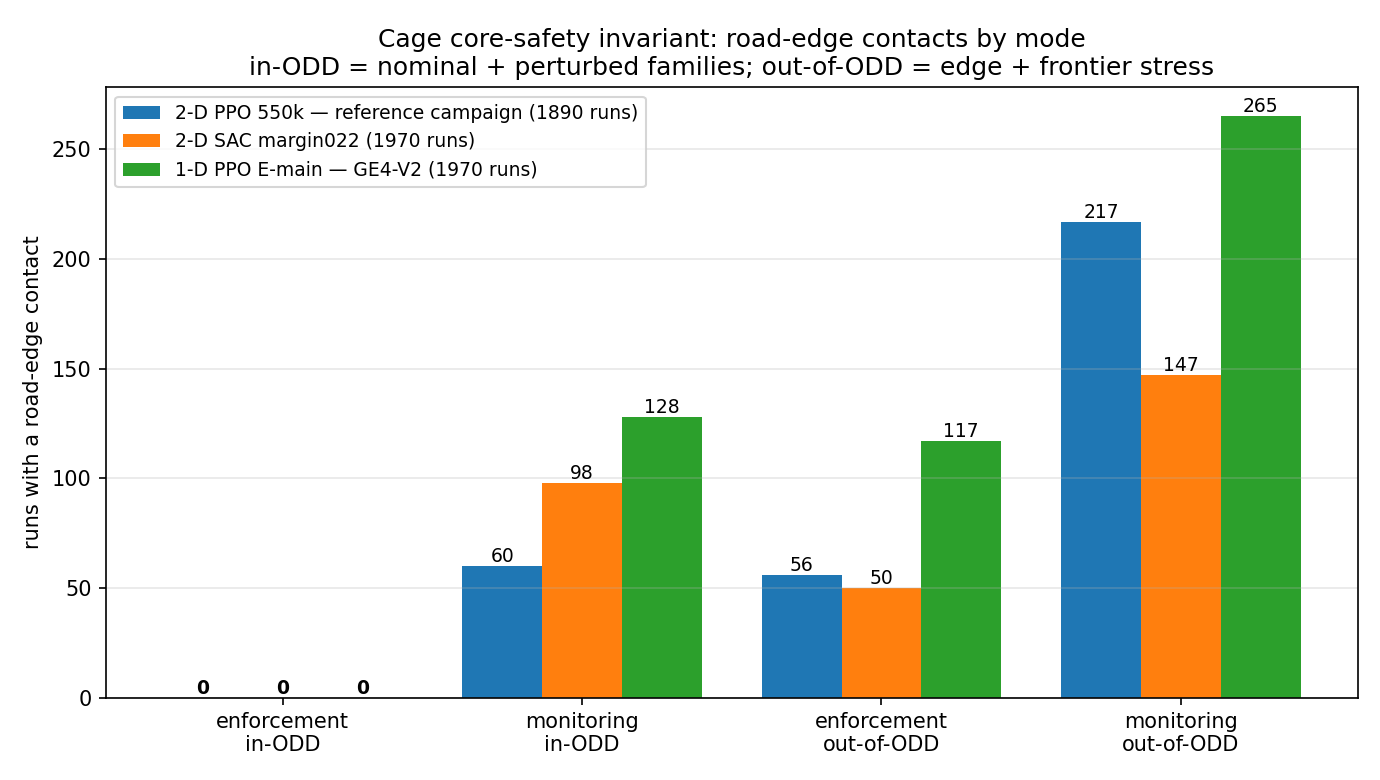
\includegraphics[width=0.90\widefigurewidth]{fig_8_1_safety_invariant.png}
  \caption[Road edge contacts by mode and by domain membership.]{Contacts with the road edge by mode and by whether the run starts inside the operational domain, for the reference campaign and the two earlier ones, \texttt{margin022} and \texttt{GE4-V2} (Table~\ref{tab:7.1}). The \enquote{inside the ODD, enforcement} block is zero in all three. The differences between policies are outside the domain.}\label{fig:8.1}
\end{figure*}

\subsection{Latent inside, active where perception gets worse}
\label{sec:8.4.1}

In the clean nominal scenario the cage is latent. The policy drives 5.32 laps with 8.6 mm mean lateral error, zero emergencies and zero safety interventions, and only the rate limiter acts. But comparing the modes scenario by scenario (Table~\ref{tab:8.4}) shows where the cage stops being latent:

% layout: table, natural, \small, 84 of 107 mm
\begin{table}[htbp]
\caption{Scenarios the cage rescues: runs passed in each mode.}\label{tab:8.4}
\small\setlength{\tabcolsep}{4pt}
\begin{tabular}{@{}lrr@{}}
  \toprule
  \tabhead{Scenario} & \tabhead{Enforcement} & \tabhead{Monitoring} \\
  \midrule
  Compound state & 30/30 & 0/30 \\
  Frontier (lateral approach) & 25/25 & 0/25 \\
  Worn markings & 25/25 & 0/25 \\
  \textbf{Degraded markings + glare} & \textbf{40/40} & \textbf{20/40} \\
  300 s endurance & 25/25 & 8/25 \\
  \bottomrule
\end{tabular}
\end{table}

This is the evidence behind the main claim. The cage removes failures that the policy makes on its own, and it does so through the intended mechanism, the controlled stop when perception is unreliable, in exactly the scenarios where the visual channel degrades. The cage does not make the driving better. It limits what happens when the driving fails.

\begin{figure*}[htbp]
  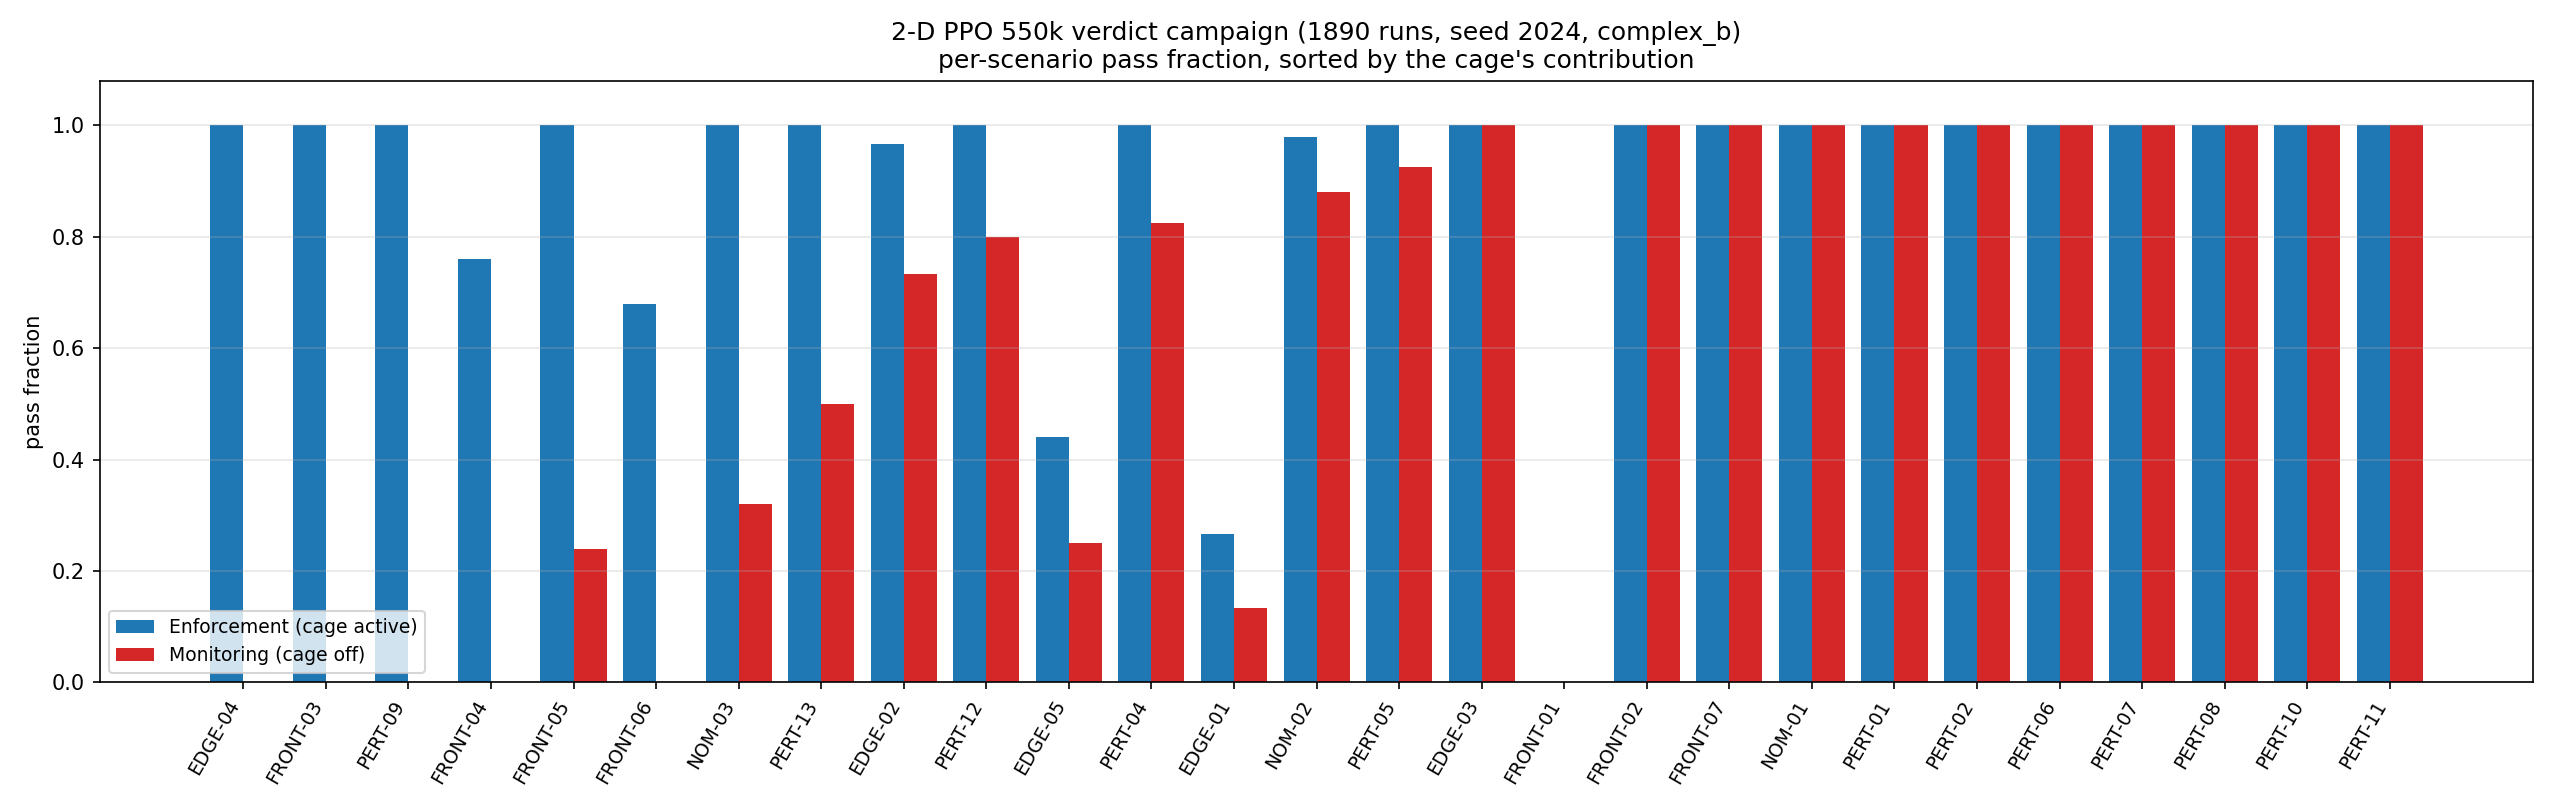
\includegraphics[width=0.96\widefigurewidth]{fig_8_2_campaign_pass_fraction.png}
  \caption[Pass fraction by scenario and mode.]{Share of runs passed per scenario in the reference campaign (\texttt{2-D PPO 550k}, Table~\ref{tab:7.1}; scenario IDs without the \texttt{SC-} prefix), enforcement against monitoring, sorted by how much the cage contributes. In the scenarios at the top, the envelope makes the difference between finishing and not finishing.}\label{fig:8.2}
\end{figure*}

\section{The uncomfortable finding: the rate limiter keeps the car in the lane}
\label{sec:8.5}

The 300 s endurance test shows a reversal that the verdict tables hide, and it turned out to be the most informative finding of the campaign. With the cage active, all twenty-five runs finish without any real excursion. With the cage inactive, seventeen out of twenty-five end off the road. None of the earlier policies, not even the worst ones, did this.

Four measurements narrow down the cause.

\textbf{It is not drift building up over time. It happens at fixed places.} The seventeen departures happen at exactly two points of the circuit, the two tightest apexes. In the last seconds before them, the jerk of the command is \emph{lower} than the run's average. It is not oscillation. It is steady, confident oversteering.

\textbf{The only difference between the modes is the rate limiter}\sidenote{\cagerule{06} caps how much the command may change from one cycle to the next: 0.15 for steering and 0.10 for throttle, on the normalised command.} (Table~\ref{tab:8.5}). Same policy, same layout, same speed at the apex:

% layout: table, natural, \small, 94 of 107 mm
\begin{table}[htbp]
\caption{Enforcement and monitoring at the apex: the only difference is the limiter.}\label{tab:8.5}
\small\setlength{\tabcolsep}{4pt}
\begin{tabular}{@{}lrr@{}}
  \toprule
  \tabhead{At the tightest apex} & \tabhead{Enforcement} & \tabhead{Monitoring} \\
  \midrule
  Raw steering command (max.) & 1.00 & 1.00 \\
  \textbf{Applied} command (max.) & \textbf{0.84} & 1.00 \\
  Applied change per cycle & $\le$ 0.15 & up to 2.0 \\
  Maximum lateral error & 36 mm & 145 mm $\rightarrow$ off the road \\
  \bottomrule
\end{tabular}
\end{table}

\textbf{No safety rule steps in.} In the twenty-five enforcement runs, the intervention log contains only the rate limiter, with zero activations of the lateral limit, heading, predictive and emergency rules. The rule that keeps the vehicle in the lane at those apexes is, on paper, a class B smoothness rule.

\textbf{This policy's raw command is about twice as abrupt} as that of the earlier policies, and it saturates the limiter in 77.5\,\% of the steps. Speed does not explain it. The previous policy drives 7\,\% slower and stays on the road, and in the comparison between modes the speed is the same because it is the same policy.

\textbf{Interpretation, and its limits.} The most likely explanation is co-adaptation.\sidenote{During training the policy only ever acted through the limiter, so jerky commands were smoothed before they could cost any reward. Nothing pushed the policy to learn smooth commands itself.} The policy was trained with the cage in the actuation chain, where the limiter smooths whatever the policy commands. In that closed loop, an almost all-or-nothing command is not penalised, so the policy produces it. With the cage active, the pair drives better than any other configuration in this work. Without it, the same command leaves the lane about once every three laps. The cage is not only filtering this policy. It has shaped what the policy learned to output.

There are two limits to this explanation. The dependency is measured, but its origin is inferred. Proving the cause would need an ablation\sidenote{An ablation removes one part, here the limiter during training, and repeats the experiment to see whether the effect goes away with it.} (retraining with the limiter out of the loop), and that has not been done. Exposure also matters. The short nominal scenario passes 50/50 in monitoring, so a short nominal evaluation cannot detect this property. Only the endurance test shows it.

This has three consequences for reading the rest of the work. \enquote{The cage is latent inside the domain} is still true for the safety rules, but it must not be read as \enquote{the cage does nothing}: for this policy, the safety rules are latent \emph{because} the limiter acts first. The class B label of the smoothness requirement underestimates what that rule is doing. And on the physical platform, where the actuator dynamics are not the simulated limiter, a policy so tied to one specific parameter of the envelope is a transfer risk. Chapter~\ref{ch:12} states this explicitly.

\section{The negative verdict: combining rules}
\label{sec:8.6}

Of the fourteen requirements, one is closed as not satisfied, and it is reported that way instead of being explained away.

Its criterion says that when two or more rules fire in the same cycle, the resulting command must stay within the safe envelope of all of them. The co-activation grid, whose starting conditions are set on purpose to force this case\sidenote{The grid is scenario \scn{EDGE-05}: 100 runs whose starting points are chosen so that two or more rules must fire in the same cycle (\S\ref{sec:I.4}).}, shows that this does not hold. Of the 85 grid points inside the domain, 16 break the lateral margin. With the previous policy it was 30 out of 85.

Looking at which rules fire together shows the problem clearly. The violations are concentrated where the lateral limit and heading rules fire together (15 out of 20 runs fail, with 11 violations) and in the triple that includes them. They are milder when the lateral rule fires with the predictive rule (4 violations). They disappear completely where lateral and heading corrections do not conflict: speed together with the rate limiter produces no violation and no failure.

Training a better policy cuts the problem in half, but it does not change what kind of problem it is. That is the main conclusion. How the cage arbitrates when rules fire together is a design property of the cage, not a defect of the policy, and the evidence is that two very different policies show the same pattern, only weaker. It is exactly the hazard the register predicted when it included a hazard for the mitigation mechanism itself, and it is kept as stated future work.

The requirement is class B, so it does not block the global verdict, and no class A safety condition is involved. Having a negative verdict in the matrix, next to the claim of zero contacts inside the domain, is what makes that claim believable.

\subsection{The two requirements closed out of band}
\label{sec:8.6.1}

Two requirements are closed on their own metric instead of through scenario results. In both cases the reason is documented.

The actuation smoothness requirement is checked directly on the trace of the command that was actually applied. In enforcement, 840 out of 840 runs stay within the per-cycle limit. In monitoring, only 263 out of 945 do. This is also the most direct measure of what the limiter is worth.

The \emph{liveness} requirement is closed on its own measurements.\sidenote{Liveness: the vehicle keeps making progress. A policy that learns to park avoids every penalty but is useless, which is hazard \hz{08}.} Its scenario, a two-arm meta-test that adds an incentive to stop, was left out of the campaign because it does not depend on the policy and had already been closed separately, with three measured parts. The nominal policy never stops. A deliberate attempt to make it stop does not work, which is positive evidence that the training mitigation works. And the detector does fire on a real stop injected by a script. So: a mitigation that works, a failure mode that is resisted, and a metric that works.

\section{Comparison with the perfect perception arm}
\label{sec:8.7}

The control arm uses the same cage and the same scenarios, but the state comes from ground truth instead of the camera. It closes with a global verdict of satisfied, and it gives a finding that puts everything above into context: with perfect perception, the cage is completely latent inside the domain. Its boundary violation metric is zero in both modes, and there is no difference between enforcement and monitoring.

Read together, the two arms give the empirical contribution of the work: how much the cage is worth depends on how good perception is. When perception is perfect, the envelope has nothing to correct, and its value only shows outside the domain. When perception is a network learning from degraded pixels, the envelope goes from latent to active and removes failures that can be measured. Without the control arm, the result of the camera arm would be unclear: it would not be possible to tell whether the cage helps because the problem is hard or because the policy is bad.

\section{Threats to validity}
\label{sec:8.8}

\begin{itemize}
  \item \textbf{One seed in the verdict campaign.} The reference campaign uses one seed. Variation between seeds is studied separately (\S\ref{sec:7.4}) and shows that behaviour is not the same across seeds. Whether the verdict holds for other seeds is not established.
  \item \textbf{One circuit.} All reference results come from one layout. The second layout of the control arm makes the argument more plausible, but it does not settle it.
  \item \textbf{Laps cannot be compared between layouts}, and lateral error cannot be compared between observation types. The work avoids these comparisons and points them out where a reader might be tempted to make them.
  \item \textbf{Simulation, not reality.} No result in this chapter is evidence about the physical platform. Chapter~\ref{ch:09} describes what is known and what is not about that step.
  \item \textbf{The origin of the dependency on the limiter is inferred}, not proved, and the ablation that would prove it has not been run.
  \item \textbf{One operational incident} during the campaign affected 222 runs: two processes wrote to the same directory at the same time. Those runs were set aside and run again under a serial driver with a lock, and the final results cover all 1,890 cells with no errors. It is recorded here because the integrity of the evidence is also a claim that needs evidence.
\end{itemize}

\section{Summary}
\label{sec:8.9}

The reference campaign gives four results. Inside the domain, with the cage active, there are zero contacts with the road edge, against sixty that the policy makes without it. The cage's safety rules are latent inside the domain and become active exactly where perception gets worse. The rate limiter does lane-keeping work that its classification does not reflect, and this dependency is a stated transfer risk. And one requirement, rule composition under co-activation, is not satisfied. It is reported as such and kept as future work.

Chapter~\ref{ch:09} looks at how much of this can be expected to survive the move to the physical platform.

% GENERATED by md2tex.py from ../draft_v5_en/body/09_sim_to_real_gap.md -- do not edit by hand.
% Change the Markdown and run `python md2tex.py`; edits here are overwritten.

\chapter{Measuring the sim-to-real gap}
\label{ch:09}

\section{The gap as a subject of study}
\label{sec:9.1}

Adaptation A5 says that operational validation must include, as a required part and not an optional one, an explicit description of the gap between the environment where the system was trained and the one where it will run. This answers an imbalance in the literature pointed out in \S\ref{sec:2.7}: there are many techniques to \emph{reduce} the gap, but few frameworks to \emph{measure} it in a way a safety argument can use.

This chapter studies the gap in steps of increasing realism: the simulator where all the verdict evidence comes from, a bridge with more realistic physics and graphics, and the real platform. Each step answers a different question, and the chapter states clearly which questions have a measured answer today and which do not.

\section{First step: the high-fidelity bridge}
\label{sec:9.2}

An equivalent environment was built in Isaac Sim, which uses the PhysX physics engine and RTX rendering and is more realistic than Gazebo in both respects. The full chain was ported: import of the vehicle model, sensor publishing, in-process training, domain randomization, and the same cage with its parameter file.

The most useful result of this step is not a campaign but a diagnosis. It should be reported as such, because it is exactly the kind of information A5 is meant to collect. Porting the system uncovered a series of problems that were not about implementation but about how the layers depend on each other. The yaw authority of the model had to be recalibrated because the dynamic response is different. The cage's heading thresholds had to be recalibrated for the new renderer, because the vision estimator reads the same lane with a different bias. And the policy with speed control found a degenerate optimum (stopping) that the earlier environment had not allowed it to show.

The main lesson of this step comes from those problems: checkpoints do not transfer between simulators. A policy trained in one is not a valid policy in the other, even with the same architecture and the same reward. Each environment needs its own training. If this happens between two simulators, expectations about moving to the physical platform should be set with that in mind. It is a negative result, and a useful one.

\section{Second step: the physical platform}
\label{sec:9.3}

\subsection{Status}
\label{sec:9.3.1}

\begin{quote}
\textbf{What follows is the \emph{bring-up} of the physical step, not its results campaign}\sidenote{Bring-up: getting the hardware chain to run end to end and calibrating it. It comes before, and is not the same as, a campaign run under the scenario protocol.}, and this should be kept in mind before reading the numbers. The physical evidence in this chapter comes in two kinds, which carry different weight. The first kind is calibration measurements and structural findings: measurements against a reference, a regression over 5,665 cycles, two controlled pairs, a threshold comparison, and a true-position capture over the whole layout. These are results and do not depend on any campaign. The second kind is driving figures, which come from runs done outside the scenario protocol and are therefore preliminary: nominal tracking from a single run (\S\ref{sec:9.3.4}), and envelope blocking from three runs (\S\ref{sec:9.3.7}). A physical campaign would replace the second kind, not the first.
\end{quote}

The physical deployment chain is built, documented end to end and running on hardware: onboard camera, policy node, lane estimator, cage node, vehicle control and platform driver, all on the real vehicle on a closed lane circuit. This step has produced evidence of three kinds that should not be mixed: calibration measurements on the hardware, a negative result about the policy that simulation had validated, and a positive result about the policy retrained for transfer.

What it has not produced is a scored scenario, for three reasons that are independent of each other. The driving was done outside the library protocol, in monitoring mode instead of enforcement, and with a perception setting different from the one used to score the campaigns. Any one of these is enough to mean that nothing in this chapter is a verdict, and all three apply. So Chapter~\ref{ch:10} marks its physical column as \emph{not executed} (\S\ref{sec:10.4}d–\allowbreak{}e), and everything that follows here is later evidence. That column should not be confused with the physical column of the gap table in \S\ref{sec:9.4}, which does contain figures. The first one scores requirements under protocol and is empty by decision. The second one compares driving quantities outside the protocol and is preliminary by definition.

\subsection{The blocking check was done, and it failed}
\label{sec:9.3.2}

The item marked as blocking was the effective field of view of the onboard camera.\sidenote{The effective field of view is the horizontal angle the camera really sees. Converting pixels to millimetres depends on it, so a wrong value scales every lateral quantity.} It was a default configuration value that the simulation had copied, so no simulation result could reveal an error in it, and every lateral quantity the cage uses depends on it. It was measured before any driving metric, as the chapter had planned, and the value was wrong: the effective horizontal field of view of the real module is 77.89°, not the assumed 90°.

The effect was then measured against a tape measure, with the vehicle moved by hand over a range of $\pm$100 mm, on the unrectified image. The estimator read the lateral error as about 0.68–0.83 times the real value minus 10 mm. This under-reading did not go away with any filtering, and it would have triggered the boundary threshold, set at 160 mm, with the vehicle at a real 207–241 mm. The lane width, on the other hand, was read correctly (252.9 mm against a 250 mm ruler). A width is a \emph{difference} measured across the optical axis, while the lateral error is an \emph{absolute position} away from it, and the lens distortion term that was not modelled only compresses the second one. This diagnosis decided the fix, and the conclusion was clear: rectify the image, do not just change parameters.

\begin{quote}
\textbf{Partial retraction, which supports the chosen fix.} The numbers in the previous paragraph describe the \emph{unrectified path} and not the deployed system. When the measurement was repeated on the rectified image (nine points, vehicle on the ground, not touched), the scale is 1.058 on the left and 0.991 on the right, and the intercept is gone. The 160 mm threshold now triggers with the vehicle at a real 151–158 mm, which leaves about 100 mm of margin to the edge instead of 14 to 48. The under-reading was real, it came from the optical path and not from the estimator, and rectification removed it. The original number is kept because it is the evidence that justified the decision. No cage rule should be tuned from it.
\end{quote}

This is exactly the kind of finding adaptation A5 exists for, and it should be said clearly. An assumption that simulation could not falsify, because simulation had inherited it, turned out to be wrong on the very first measurement on hardware, and it sat in the path of a safety rule. The chosen fix is not to change the estimator's parameters but to rectify the real image to the standard camera model\sidenote{Rectifying removes the lens distortion, so that the image follows the same ideal pinhole camera model that the simulator uses.}, so that one projection works for both the simulation campaigns and the vehicle. Its effect was measured on hardware with the car stopped and untouched: cycles with invalid perception drop from 45\,\% to 5.5\,\%, and the lane boundary rule goes from firing 102 times without the car moving to not firing at all. The nine-point measurement above confirms this in the range that matters.

\subsection{The policy validated in simulation does not transfer}
\label{sec:9.3.3}

The first real drive with the reference policy, the two-dimensional one that the verdict campaign had evaluated, gave a clear negative result. The vehicle was moved by hand over a range of 332 mm of lateral error, with the chain running but not driving the motors, over 5,665 logged cycles. The steering command reacts to the position with the correct sign, but ten times too weakly. The change in steering across the whole 332 mm is 0.055, while there is a constant bias to the left of 0.1155, which is 2.1 times that whole change. Only 29 of the 5,665 samples (0.5\,\%) ask for a right turn. In closed loop the bias wins, and the vehicle leaves the lane to the left wherever it starts.

The cause of the bias is the training circuit itself. Driven clockwise, each lap has about 13 m of left curves and 2 m of right curves, a ratio of 6.5 to 1, and the training action log shows the mean steering flat at +0.112\ldots{}+0.120 over all 284,672 steps. It is not a perception or dynamics problem. The policy memorised the handedness of the track as a steering bias.\sidenote{Handedness is the balance between left and right curves. Driven clockwise, \texttt{complex\_b} has about 13 m of left curves and 2 m of right curves per lap.} This is a property of the training distribution, and no appearance randomization would have fixed it.

\subsection{Retraining for transfer, and the result}
\label{sec:9.3.4}

The gap was split into three separate terms, and only the first one is a property of the track. Handedness: observation and action are mirrored per episode\sidenote{Mirroring flips the image left to right and the sign of the steering together, so in about half of the episodes the policy effectively drives a right-handed circuit.}. Photometry: three quarters of the episodes use the lighting range measured in the hall. Camera geometry: mount pitch, height and, in one tenth of the episodes, the real measured lens. A new policy was trained on this basis for 2.5 million steps.

The deployed checkpoint is not the one with the highest reward. It was chosen on two criteria: how well it responds under deployment conditions, and how little it depends on the cage. The chosen candidate triggers the rate limiter in 3.0\,\% of nominal cycles, against 35.0\,\% for the reward peak. The second criterion was chosen on purpose. The transfer risk stated in Chapter~\ref{ch:08} was exactly the policy's dependence on the limiter, so a checkpoint that relies on it is the wrong one to put on hardware. This is the second time in this work that the reward curve picks badly.

The handedness term was fixed: the bias/excursion ratio drops to 0.07–1.10, against 12.9–19.2 for the reference policy as it was deployed.

\textbf{And it transfers: first measurement, one run.}\prelimflag{} The retrained policy drove 18.05 m of the real circuit in one continuous segment of 101.1 seconds, with no operator help. Its median lateral error was 18.7 mm (maximum 98.7 mm, against a boundary threshold of 160) and its maximum heading error was 18.91°, against a limit of 25. No safety rule fired during the run. The only rule that acted was the rate limiter, in 3.4\,\% of moving cycles, against 3.0\,\% measured in simulation.

That last pair of numbers is the most important observation of the bring-up, because it is the first measurement of a question Chapter~\ref{ch:08} left open. The transfer risk identified in advance was that the physical actuator does not apply the per-cycle change limit that the policy had come to rely on, so the pair \emph{(policy, limiter)} might not survive on hardware. In the first run it did, with the two numbers only four tenths of a percentage point apart. One run does not rule out the risk, and the campaign could still show it. But the difference is not borderline, and it goes in the opposite direction from the one feared. The framework asked for the risk to be stated before touching hardware and for the first measurement to test it, and that is what happened. Closing it needs the campaign.

\subsection{What stops the vehicle is not the policy}
\label{sec:9.3.5}

The run ended 2.11 m before completing the circuit, and the reason had nothing to do with driving. A single 400 ms pulse of invalid perception, which the estimator recovered from on its own, latched the emergency stop\sidenote{Latched: once \cagerule{05} fires it stays active until an explicit reset, even after the trigger has gone. This avoids switching on and off at the edge of the trigger.} while the vehicle was 27 mm from the lane centre, on the tightest curve of the layout. Because the rule's exit is asymmetric, it stayed latched for the remaining 396 s. The rule did exactly what its specification says: to exit, it needs an explicit reset. That decision came from the hazard analysis, to avoid switching back and forth at the edge of the trigger. The gap is not in the cage. It is between an artefact validated on simulated episodes, which end, and a vehicle that has to keep running. It was solved by leaving the rule as it is and placing the reset path outside the cage. This was done on purpose, so as not to change the artefact under verification with a change whose whole effect is on hardware and that simulation could not validate, because in simulation the latch hardly ever matters.

There are two more findings of the same kind, and neither involves the policy. When the stereo camera's visual odometry closes a loop\sidenote{Loop closure: when the camera recognises a place it has already seen, it corrects its accumulated drift in a single step. That step is what reaches the cage as a pose jump.}, it resets its pose and jumps. Since the state filter fuses that pose and not its velocity, the jump reaches the cage as a velocity spike. A displacement of 3.6 m in one frame and a velocity of 5.5 m/s were measured, against a contract speed of 0.22. This triggers the chain of speed rules and ends the run. Turning off loop closure removes the problem: jumps per frame go from 116 to 0 in 509 s. The second finding is that the cage's speed ceiling cannot fire on commanded motion in the deployed configuration, because its threshold (0.25 m/s) is higher than the operating speed (0.22 m/s). What Chapter~\ref{ch:08} recorded as a coverage gap in the campaign is, on hardware, a rule that does not protect the real case: the vehicle enters the tightest curve at contract speed with no speed protection from the cage. The audit of the caged runs adds the opposite problem, which is even more uncomfortable. The rule did fire, 58 and 40 cycles in the two runs that passed the audit, and 100\,\% of those were caused by velocity errors from the pose sensor (0.25–1.30 m/s reported, which the vehicle cannot reach under its own power). In one of the runs, these false activations blocked the reset path of the very rule they had triggered. A rule that does not act on the case that exists, but does act on one that does not, is a different finding from a coverage gap. The failure is not in the rule itself but in how its threshold, the chosen operating point and the quality of its only speed input fit together. It is documented and not fixed, because turning it back on would first need a reliable curvature signal (\S\ref{sec:9.3.6}).

\subsection[How accurate the estimator is depends on where the car is, not on how it moves]{How accurate the estimator is depends on \emph{where} the car is, not on how it moves}
\label{sec:9.3.6}

With the geometry fixed, the estimator still kept stopping the vehicle. The cause was found with a deliberately low-tech measurement: four stations marked with tape on the floor, the vehicle pushed by hand with a pointer on the chassis following the painted line, and only the camera running (no policy, no cage, no odometry). There were four laps and four tests with the vehicle stopped, about 11,500 frames in total. The acceptance criterion was set before measuring and is based on a geometric fact that does not depend on odometry: on a closed circuit, the curvature integrated over one lap equals 2$\pi$\sidenote{Over one closed lap the heading turns through one full circle, whatever the shape of the circuit. The check needs no reference position, and the measured values are ratios to that expected total.}.

The criterion fails by a factor of two. The integration gives 1.97 / 2.01 / 2.25 / 2.37, against an acceptable range of 0.75–1.35. This is the first measurement of the curvature channel that does not depend on the vehicle or its state estimation. But the result that changes the order of the work is a different one: the estimator does not get worse because of driving, it gets worse depending on where it is. At the start of the straight, it pairs 96.7\,\% of the frames and is off by 7.2 mm. On the sections in between, it pairs between 37.9\,\% and 60.2\,\%. With the vehicle stopped at two of those points and the true lateral error at zero, one test pairs 0.0\,\% of its 273 frames, and another pairs 100\,\% with a bias of $-$39.7 mm and a standard deviation of 3.1 mm. In other words, it is confidently wrong, so no check based on spread can catch it.

This has two consequences for the method, and both change what was written earlier. The first is that the start of the straight, where the field of view calibration, the nine-point measurement and all the pre-deployment checks were done, turns out to be the best point of the circuit for the estimator. The content of those measurements still holds, but they can no longer be taken as valid for the whole layout. The second is about the mechanism. The problem is not choosing the wrong pair among candidate lines. It is in how the candidates are generated: edges of the same stripe, nearby markings, or a single visible line. The pair that survives has a plausible width, but its midpoint is shifted. A check for continuity over time on the chosen pair would not fix this, because the wrong pair is stable to within 3.1 mm.

\subsection{The three cage blockages, measured}
\label{sec:9.3.7}

The claim in \S\ref{sec:9.3.5}, that what stops the vehicle is not the policy, was tested in three runs in a row on the real circuit, all in monitoring mode, changing only the settings of the reset path. None of them kept the vehicle moving, and all three failed because of measurement, not driving.

The first run shows that the requirement of one second of healthy perception cannot be met while moving. Nine resets were issued, and the log contains 623 that were denied. 48\,\% of those were denied because the wait never completed, since the estimator's health signal flickers faster than once per second. That threshold came from a hazard analysis argument against switching at the edge of the trigger, and it had never been tested with the vehicle moving. The second run tests the documented way out (removing the lane boundary rule from the blocking set) and rules it out. The budget of thirty resets is used up in about one minute, each one latching again immediately, with the vehicle stopped and the estimator reading a lateral error of $-$296 mm. A denied reset just becomes a wasted reset. It is not a way out. The third run shortens the wait and finds the next thing that blocks: over the 1,066 cycles in which it acts, the heading rule fires with the vehicle 20 mm from the lane centre and a heading standard deviation of 19.1°, against a threshold of 25°. The same configuration, measured at the start of the straight, gave 5.3°.

That last comparison is the important one. It is the fourth independent confirmation of \S\ref{sec:9.3.6}, and the first in the heading channel with the vehicle driving: heading gets worse away from the good spot, in the same way as offset and curvature. The three blockages do not show a policy that cannot drive. They show the stopping rule firing on a measurement that fails exactly where \S\ref{sec:9.3.6} said it fails. That is why the remaining work puts the estimator before the policy.

\subsection{Experimental design still to do}
\label{sec:9.3.8}

The physical subset of the library (nominal, and nominal with curvature and heading limit, in both operating modes) has still not been run under protocol, and four conditions stand in the way. Three were identified before driving and are about instrumentation and contract: a reset path for the emergency stop, per-run provenance logging (already implemented), and a decision on which perception contract to use, because the heading setting that lets the vehicle drive is not the one the campaigns were scored with. They are listed with their criteria in \S\ref{sec:12.4} (T2), which is where the work hands them over.

What should be stated here is which of the four matters most, because it is a result of this step and not an inherited task. The fourth one was added by the hardware: widen the lane estimator before restricting the policy. The estimator's accuracy depends on the point of the circuit (\S\ref{sec:9.3.6}), and its failure is what actually blocks the vehicle (\S\ref{sec:9.3.7}). Until this is fixed, a scored run would measure the envelope on an input that is known to be faulty in areas the vehicle normally drives through. Only one parameter of the operational domain is meant to be closed at this step, and only here: the lateral acceleration envelope, which cannot be measured in simulation at all. It is still open.

\section[The gap table (preliminary physical column)]{The gap table \emph{(preliminary physical column)}}
\label{sec:9.4}

The table now has a physical column\prelimflag{}, and the first thing to notice is not a row but a column heading: the deployed policy is not the one that produced the simulation verdict. That change is itself a result of this step (\S\ref{sec:9.3.3}). It means the physical column and the simulation columns are not a like-for-like comparison. They describe different policies, in different modes, under different perception contracts. They are shown together because the comparison still tells something useful, and they are separated in their headings because treating them as a clean difference would be exactly the kind of unsupported claim the framework is meant to prevent.

% layout: table*, fixed, \small, 164 of 165 mm
\begin{table*}[htbp]
\caption[Gap table. The two simulation columns describe the verdict policy.]{Gap table. The two simulation columns describe the verdict policy. The physical column is preliminary (the policy retrained for transfer, in monitoring, over one run, with no scored scenario) and the physical campaign will replace it.}\label{tab:9.1}
\small\setlength{\tabcolsep}{4pt}
\begin{tabular}{@{}>{\RaggedRight\arraybackslash}p{24.9mm}>{\RaggedRight\arraybackslash}p{27.9mm}>{\RaggedRight\arraybackslash}p{39.1mm}>{\RaggedRight\arraybackslash}p{63.2mm}@{}}
  \toprule
  \tabhead{Metric (nominal scenario)} & \tabhead{Sim 1-D \emph{(historical reference)}} & \tabhead{Sim 2-D \emph{(the one that produced the verdict)}} & \tabhead{\textbf{Physical} \emph{(PRELIMINARY: retrained policy, monitoring, \textbf{one run}, unscored)}} \\
  \midrule
  Median lateral error & 10.9 mm & 8.6 mm (max. 27.3 mm) & 18.7 mm (max. 98.7 mm) \\
  \addlinespace[2pt]
  Continuous run & 4.88 laps & 5.32 laps & 18.05 m in one segment ($\approx$ 0.94 of the perimeter) \\
  \addlinespace[2pt]
  Maximum lateral excursion & < limit over the whole domain & 0 edge contacts inside the ODD & 0 contacts; max. 98.7 mm against a threshold of 160 \\
  \addlinespace[2pt]
  Emergency stops & 0 & 0 & 1, from perception, with the vehicle in the lane \\
  \addlinespace[2pt]
  Intervention rate & 43.5\,\% (limiter only) & 3.0\,\% at the deployed checkpoint & 3.4\,\% (limiter only) \\
  \addlinespace[2pt]
  Operating speed & 0.200 m/s fixed & $\approx$ 0.216 m/s under a 0.22 ceiling & $\le$ 0.213 m/s under the same ceiling \\
  \addlinespace[2pt]
  Control loop rate & 10 Hz nominal & 10 Hz nominal & 8.68 Hz measured; 9.6 Hz after removing the lidar from layer 2 \\
  \bottomrule
\end{tabular}
\end{table*}

Three observations. First, the row that held the most risk no longer does. Chapter~\ref{ch:08} named the limiter's intervention rate as the first gap to watch, because what transfers is not the policy alone but the pair of policy and limiter, and the physical actuator does not apply that limit. With the checkpoint chosen for independence from the cage, the two numbers differ by four tenths of a percentage point. The risk was correctly identified, and the way it was handled (choosing by independence, not by reward) worked.

\textbf{The lateral error doubles, which was expected.} It is 18.7 mm against 8.6 mm in simulation, with a loop running at 8.68 Hz instead of the 10 Hz the policy was trained for, and with an estimator whose accuracy depends on the point of the circuit (\S\ref{sec:9.3.6}). It stays well within the cage threshold, and the number to watch is the 98.7 mm maximum, not the median. It cannot be claimed that this maximum hides a larger real value because the estimator under-reads: on the rectified path the scale is practically one (\S\ref{sec:9.3.2}). The bias that does remain is the one that depends on place. It can go in either direction, and without true-position measurements it cannot be applied row by row.

\textbf{The loop rate is still open, but it is no longer the main gap.} It is the only parameter of the deployment contract that the hardware does not reach. Its cause has been found: not the camera, which delivers 9.84 Hz, but the network's inference time. It has been improved from 7.3 to 9.6 Hz, but not closed.

\section{Summary}
\label{sec:9.5}

The chapter leaves the gap clearly described, and in a different state from before. The first step is measured, and its result is still a useful negative diagnosis: checkpoints do not transfer between simulators, and perception, calibration and dynamics depend on each other more than the modular architecture suggests. The second step ends with the bring-up done and the results campaign not done, and it is better to say that directly than to present it as a measurement in progress. Even so, the bring-up produced five things that simulation could not, and four of them do not depend on the campaign being run.

It produced a falsified assumption: the field of view that simulation had inherited from a default setting was wrong, it sat in the path of a safety rule, and no amount of extra simulation would have shown it. It produced a negative result about the validated policy: it does not transfer, and the cause, the handedness of the training circuit memorised as a steering bias, is a property of the training distribution and not of the hardware. It produced a positive result about the replacement policy, and with it an answer to a transfer risk stated in advance. It located a failure mode that simulation cannot show at all: the lane estimator's accuracy depends on the \emph{place} on the circuit and not on what the vehicle is doing. This was measured with true-position methods and later confirmed independently in the heading channel while driving. And it produced a kind of finding that only appears with a real vehicle in front of you: rules that are correctly specified but have no defined behaviour in operation, thresholds that cannot fire in the deployed configuration, and sensors whose failures go straight into the cage's only speed input.

There is also a result about the method, which only becomes visible when all the gap terms are put into one table. This work can state it because it wrote its list of gaps \emph{before} touching hardware and did not edit it afterwards. That early list got four terms right (appearance, provisional thresholds, computation rate and yaw gain), and they are all of the same type: terms that a simulator knows how to represent. Nothing that actually stopped the vehicle was on that list: the handedness of the training circuit memorised as a bias, an intrinsics error that the simulator had inherited and so could not reveal, an estimator whose accuracy depends on place and not on action, a correctly specified latch with no defined operational behaviour, and a sensor whose failures go straight into the cage's only speed input. Three of these five are in the measurement chain (the camera intrinsics, the lane estimator and the speed sensor), one is a property of the training distribution, and one is about how a rule behaves in operation. None of the five is the control policy. This imbalance is the chapter's methodological finding: the gap terms a team working in simulation can list in advance are exactly the ones simulation knows how to model (appearance, timing, gains), and the ones that stopped this vehicle are the ones simulation had no representation of at all, either because it inherited the same assumption, because the quantity does not exist there, or because its plant is better than the real one.

Adaptation A5 is met for the first half of its requirement, which is to make the gap explicit and organise how it is measured. The second half has started but is not finished: there are measurements on hardware, but from bring-up and not from a campaign, so there is no per-scenario gap table and no physical verdict. That, and nothing else, is why the verdict column in Chapter~\ref{ch:10} is marked not executed. Chapter~\ref{ch:10} gives the final verdict with this limitation built into its statement, and with one clarification it could not make before: the limitation is no longer \enquote{there is no physical evidence} but \enquote{the physical evidence comes from bring-up and is not scored}.

There is one more point that none of the above covers, and Chapter~\ref{ch:10} includes it in its statement: the envelope has never acted on the real vehicle. All physical runs were done in monitoring mode, with the safe action equal to the raw action in every logged cycle. The central artefact of this work is verified in simulation and only \emph{observed} on hardware, and the campaign that would change that is the first item of future work.

% GENERATED by md2tex.py from ../draft_v5_en/body/10_operational_validation.md -- do not edit by hand.
% Change the Markdown and run `python md2tex.py`; edits here are overwritten.

\chapter{Operational validation}
\label{ch:10}

\section{Purpose of the chapter}
\label{sec:10.1}

The earlier chapters produce measurements. This chapter turns them into a validation statement that includes its own limits. It is the first half of adaptation A5 in practice: the conclusion is no longer \enquote{the system is safe} but a bounded claim about which requirements are met, in which domain, with what evidence, and with which residual risks stated.

\section{The evidence}
\label{sec:10.2}

The statement is based on three sets of evidence. All of them have version-controlled artefacts, and every run records its reproducibility metadata: code revision, cage configuration identifier, checkpoint identifier, seed and timestamp.

The perfect perception arm gives 1,260 runs with a global verdict of satisfied. It works as a control, because it shows what happens when perception is not a problem. The camera arm gives the scenario campaigns on a policy that learned from pixels, and ends with the reference campaign of 1,890 runs without errors that supports the verdict of this chapter. The study of variation between seeds shows that behaviour is not the same when the training procedure is repeated.

\textbf{Physical evidence exists, but it comes from bring-up and is not verdict evidence.} The chain has run on the real vehicle and has driven 18.05 m of the circuit in one segment without triggering any safety rule (Chapter~\ref{ch:09}). However, no run was done under the scenario library protocol, in enforcement mode, and with the perception contract used to score the campaigns. For that reason the physical column of the table below is marked not executed.\sidenote{Not executed rather than pending: no measurement is in progress, and no data taken outside the protocol is used to fill the column.} This is more precise than saying that there is no data. Having driven is not the same as having scored, and filling the column with measurements taken outside the protocol would be exactly the kind of claim the framework is meant to prevent. The limits this imposes are stated in \S\ref{sec:10.4}d–\allowbreak{}e.

\section{Final verdict table}
\label{sec:10.3}

% layout: table*, fixed, \small, 164 of 165 mm
\begin{table*}[htbp]
\caption[Final verdicts per requirement.]{Final verdicts per requirement. The physical column is not scored in this work: no run on hardware was done under the scenario protocol, and all of them were done in monitoring mode (\S\ref{sec:10.4}e). It is marked \enquote{not executed} and not \enquote{pending}, so as not to suggest a measurement in progress.}\label{tab:10.1}
\small\setlength{\tabcolsep}{4pt}
\begin{tabular}{@{}>{\RaggedRight\arraybackslash}p{41.2mm}>{\centering\arraybackslash}p{10.6mm}>{\RaggedRight\arraybackslash}p{25.9mm}>{\RaggedRight\arraybackslash}p{49.7mm}>{\RaggedRight\arraybackslash}p{24.9mm}@{}}
  \toprule
  \tabhead{Requirement} & \tabhead{Class} & \tabhead{Control arm} & \tabhead{\textbf{Camera arm (reference campaign)}} & \tabhead{Physical \emph{(out of scope — \S\ref{sec:12.4} T2)}} \\
  \midrule
  \sr{001} lateral deviation & A & Satisfied & Satisfied & not executed \\
  \addlinespace[2pt]
  \sr{002} heading stability & A & Satisfied & Literal: fail (recovery clause); own criterion: satisfied & not executed \\
  \addlinespace[2pt]
  \sr{003} predictive time to departure & A & Satisfied & Literal: fail (same clause); own criterion: satisfied & not executed \\
  \addlinespace[2pt]
  \sr{004} speed ceiling & A & Satisfied & Satisfied (rule not activated in the campaign; see \S\ref{sec:10.4}b and \S\ref{sec:10.4}f) & not executed \\
  \addlinespace[2pt]
  \sr{005} emergency stop & A & Satisfied & Satisfied & not executed \\
  \addlinespace[2pt]
  \sr{006} actuation smoothness & B & Satisfied (own metric) & Satisfied (840/840 in enforcement) & not executed \\
  \addlinespace[2pt]
  \sr{007} state validity & A & Satisfied & Satisfied & not executed \\
  \addlinespace[2pt]
  \sr{008} external stop & A & Satisfied & Satisfied & not executed \\
  \addlinespace[2pt]
  \sr{009} \emph{liveness} & B & Documented abstention & Satisfied (own measurements) & not executed \\
  \addlinespace[2pt]
  \sr{010} rule composition & B & Documented abstention & Not satisfied — finding, does not block & not executed \\
  \addlinespace[2pt]
  \sr{011} heading variance & B & Satisfied & Literal: fail (same inherited clause); own criterion: satisfied (3.77° < 5°) & not executed \\
  \addlinespace[2pt]
  \sr{012} following under a degraded camera & A & n/a & Satisfied & not executed \\
  \addlinespace[2pt]
  \sr{013} safe perception degradation & A & n/a & Satisfied & not executed \\
  \addlinespace[2pt]
  \sr{014} estimator plausibility & A & n/a & Satisfied & not executed \\
  \bottomrule
\end{tabular}
\end{table*}

\begin{figure*}[htbp]
  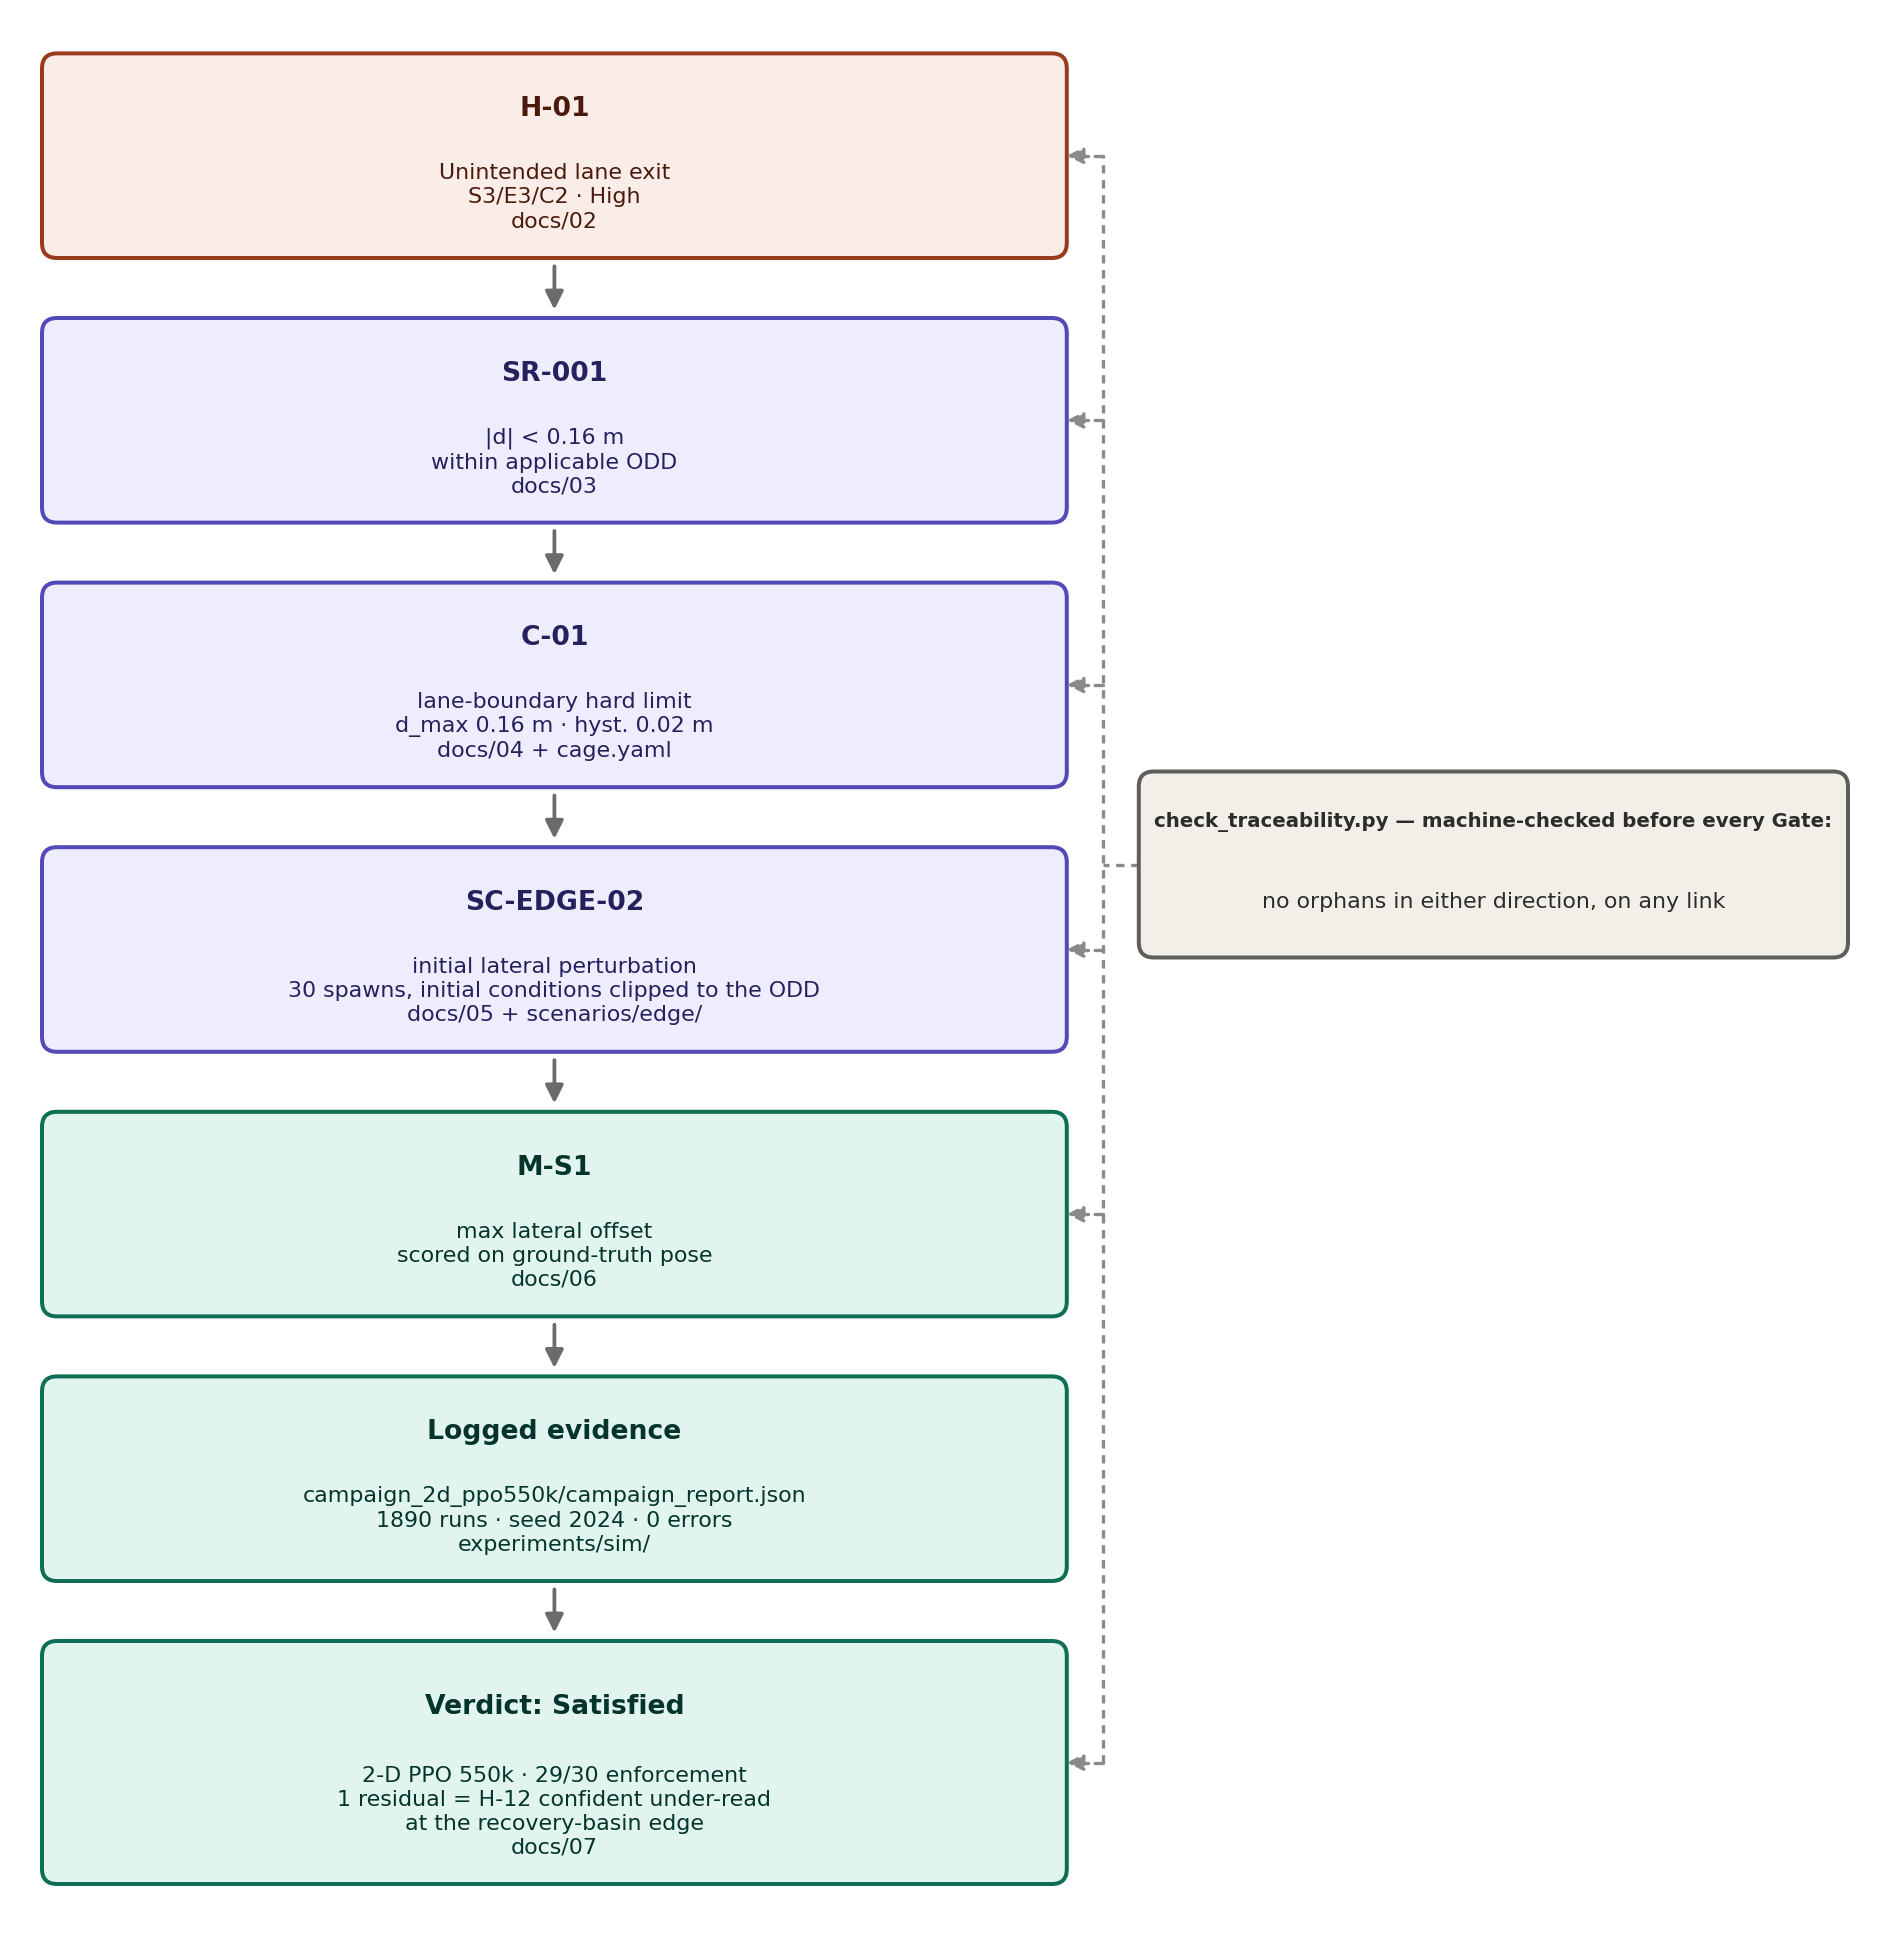
\includegraphics[width=0.84\widefigurewidth]{fig_10_1_traceability_case_sr001.png}
  \caption[The traceability chain instantiated end to end.]{One row of Table~\ref{tab:10.1} followed backwards to the evidence behind it: the chain \texttt{Hazard → Requirement → Rule → Scenario → Metric → Evidence → Verdict}, shown for the most important requirement. Every link is an identifier in a versioned artefact, and \texttt{check\_\allowbreak{}traceability.\allowbreak{}py} blocks the review gate if an orphan appears in either direction. This is how a cell of the table becomes auditable. The evidence is the reference campaign (\texttt{campaign\_\allowbreak{}2d\_\allowbreak{}ppo550k}, \texttt{2-D PPO 550k}; Table~\ref{tab:7.1}).}\label{fig:10.1}
\end{figure*}

Seen in groups: thirteen of the fourteen requirements are satisfied on their documented criterion. One is not, and it is class B, so it does not block the verdict; it is reported as it is, without being explained away. None is left without a verdict, left out of the table, or pending in the simulation column. The coverage criterion from the framework evaluation, which asked for a verdict on 100\,\% of the requirements even when the verdict is uncomfortable, is met, including that uncomfortable verdict.

Two groups of cells need a comment. The three requirements with a literal failure (\sr{002} and \sr{003} in class A, \sr{011} in class B) all fail through the same inherited clause of \S\ref{sec:8.3.2}; they keep that failure in the record next to the explanation, and are not rewritten. And the speed ceiling is marked satisfied with an important condition, explained below: it is satisfied without ever having been tested.

\section{Bounded validation statement}
\label{sec:10.4}

\begin{quote}
\textbf{Statement.} Within the specified operational domain, on a single circuit in simulation, with the two-dimensional camera policy chosen by closed-loop evaluation and with the cage configuration identified by its \emph{hash}, the system meets thirteen of its fourteen safety requirements on their documented criterion. The literal global verdict of the campaign is \verdictnot{}, and it is caused entirely by one performance clause, the heading recovery time, in one scenario, without any class A safety condition being broken.

\textbf{Inside the operational domain and with the cage active, there is no contact with the road edge} over the 555 enforcement runs that start inside it. The same policy without the cage makes sixty over those same 555. The claim is bounded to the domain on purpose: the 390 enforcement runs that start outside it still contain 56 contacts (Table~\ref{tab:8.3}). The requirement that is not met is the one on consistent rule composition when rules fire at the same time. It is class B, it was measured on two different policies, it was reduced by half with better training, and it stays the same in kind. It is stated as a design limitation of the envelope and as future work.
\end{quote}

\textbf{Explicit limits of this statement.} They are listed here, as part of the statement and not in a separate section, because each one limits a specific claim made above.

\textbf{(a) Scope.} The statement is valid in simulation, on one circuit, and with one seed in the verdict campaign. Variation between seeds is studied separately and is not uniform.

\textbf{(b) What was not tested.} The cage's speed ceiling did not fire once in the 1,890 runs, because the policy's operating speed stays below the lower limit of that envelope. The requirement is satisfied trivially\sidenote{Trivially satisfied: the requirement was never challenged, because the speed never reached the rule's threshold, so its rule was never exercised.}, and its rule has never been tested from above. This is a limitation of the operating point, not of the specification, and it is stated so that it is not read as evidence of robustness.

\textbf{(c) The measured dependency.} For this policy, staying in the lane on the tightest curves depends on the rate limiter. The dependency is measured, and its origin is inferred.

\textbf{(d) Transfer.} Physical evidence exists but is not scored, so no claim in this statement applies to the real platform. Chapter~\ref{ch:09}, and not this section, makes the one claim that can be made: the policy behind this verdict does not transfer to the real vehicle, and the one that does transfer is a later retraining. The system validated in this statement and the system that drives on hardware are not the same.

\textbf{(e) What the hardware has not tested at all, which is the biggest limit of this work.} All physical runs were done in monitoring mode. In that mode the cage checks, publishes and logs its rules, but it does not change the action, so the safe action is identical to the policy's raw action in every logged cycle. The envelope has therefore never acted on the real vehicle. The physical step measures what the cage \emph{would have said}, plus the availability cost of its emergency latch. It does not measure how the cage changes the trajectory of a physical vehicle, which is exactly the property this statement certifies in simulation. This is a limit of scope and not a negative result. There is no physical evidence against the envelope and none in its favour, and there will be none until a scored run is done in enforcement mode.

\textbf{(f) One rule that the hardware did test.} The speed ceiling is marked satisfied here without having fired once, and \S\ref{sec:9.3.5} adds two physical measurements that limit this cell without re-scoring it: in the deployed configuration the rule cannot fire on commanded motion, and the only times it did fire were caused by velocity errors from the pose sensor. For this statement that means one specific and limited thing: the verdict on this requirement depends entirely on the fact that its trigger condition was never reached in simulation, and not on evidence that the rule acts correctly when it is reached. It is the requirement with the weakest support in the table, and it is marked as such.

\section{Relation to the methodological thesis}
\label{sec:10.5}

The statement above is what the framework promised to produce: not a yes-or-no judgement, but a bounded statement that can be traced back to its evidence and that states clearly what it does not cover. Its form matters as much as its content, because that is what separates an honest validation from an approval. Every claim can be followed back to a set of logged runs, and every limit is written inside the statement rather than in a separate section a reader in a hurry could skip. The three unfavourable results — a negative global verdict, an unmet requirement and a rule that was never tested — are all inside it, and Chapter~\ref{ch:11} evaluates what that says about the framework.

% GENERATED by md2tex.py from ../draft_v5_en/body/11_discussion.md -- do not edit by hand.
% Change the Markdown and run `python md2tex.py`; edits here are overwritten.

\chapter{Discussion}
\label{ch:11}

\section{Purpose and method}
\label{sec:11.1}

This chapter evaluates the framework, not the system. This follows from \S\ref{sec:3.2.1}, where the work was presented as design science research: the object being judged is the adapted V-Model, and the lane-following system is the tool used to test it. The method was fixed in advance in \S\ref{sec:3.7}, with five criteria and their indicators, plus an evaluation of the three hypotheses from Chapter~\ref{ch:01}. Setting the criteria before knowing the results is what makes this evaluation more than a defence.

\section{Evaluation against the five criteria}
\label{sec:11.2}

\textbf{(1) Traceability integrity. Criterion: zero orphans. Met.} The checker found no orphans at any review gate or in the final matrix. What matters is not the final zero but the fact that the constraint worked as a hard gate during development: orphan identifiers were caught when they were added, not in a later audit. A zero obtained in a final audit would only show how careful the author was. A zero maintained continuously shows a property of the framework.

\textbf{(2) Requirement coverage by evidence. Criterion: 100\,\% with a verdict, even a negative one. Met.} All fourteen requirements have a verdict supported by quantitative evidence. The rule that an honest verdict is better than a missing one was applied in three ways. The global verdict of the camera arm was recorded as literally negative. Two requirements keep their literal failure next to the explanation instead of being rewritten. And one requirement is closed as not satisfied, with its measurement and a breakdown by rule combination. The criterion was met not in spite of the uncomfortable results but through them.

\textbf{(3) Hazard anticipation. Criterion: most of what was observed had been predicted, and what was not can be audited. Mostly met, and only partly tested by the physical step.} Almost every hazard that appeared was already in the register from the analysis phase, or was added when the camera track started, before the campaign measured it. Two cases were not predicted. The first is the conflict between the cage and its own estimator, where the envelope makes a competent policy worse because of a reading that is confident but wrong; its root cause was registered as a hazard, but not this way of appearing. The second is the degenerate optimum of stopping, which appears when the policy is given control of speed: the register predicted the family, reward exploitation, but the specific case had to be discovered. In both cases the framework handled the new case through the planned path of identifier, recorded decision and artefact.

A third unexpected case needs its own mention, because the framework did not predict it in any form: the dependence on a class B rule to stay in the lane (\S\ref{sec:8.5}). The hazard register considers that the cage may fail, arbitrate badly or read badly. It does not consider that the policy may adapt to the cage so much that it needs the cage in order to drive. This is a failure mode of the \emph{coupling} between the learned component and the envelope, and it suggests a hazard category that the original analysis did not have.

\textbf{The physical step tests this criterion more severely than simulation did.} On hardware the failures fall into two groups, which say different things. The first group is failures of families that were already registered but took a form the register did not describe. The register considers that the cage estimator may read badly and with high confidence, but it does not consider that its accuracy may depend on the place on the circuit (\S\ref{sec:9.3.6}). Because the family had been predicted, the case could be handled; because its form had not, it had to be measured before anything could be done. The second group is not about hazards at all, and the criterion covers it only by omission: rules that are correct according to their specification but have no defined \emph{behaviour in operation}, and thresholds that cannot be reached in the deployed configuration. A hazard register asks what can go wrong. It does not ask what happens next, and it does not ask whether the operating point ever reaches the envelope that was specified.

The honest reading is therefore that the criterion is met in simulation and only partly tested on hardware. No physical failure required a new hazard family, several required a new description, and the most uncomfortable type, which is the gap between specification and operation, lies outside what the tool can see. \S\ref{sec:9.5} measures the same point from the other side.

\textbf{(4) Adoption cost. Criterion: in proportion to the benefit. Met, provisionally.} The record holds more than seventy decisions, the checker, the templates and a dozen living documents. One person kept all of them up to date \emph{while} two training tracks, several evaluation campaigns and a bridge between simulators were being run. The exact split between framework work and technical work was not measured in hours, which was a limit stated in advance. The recorded indicator is that no review gate was delayed by framework artefacts, while some were delayed for technical reasons.

\textbf{(5) Usefulness of the matrix. Criterion: documented cases where it made the impact analysis faster. Met, with a counterexample.} There are three cases. The defect in the criterion that caused the literal negative verdict was found in minutes by following the row requirement $\rightarrow$ scenario $\rightarrow$ clause, because the chain existed. Re-scoring a requirement on its own metric was possible because the matrix showed which scenario tests which requirement with which metric. And moving the library to a new layout reused the existing chains, with changes that could be audited.

The counterexample is recorded with the same weight, because it shows a real limit. The matrix did not detect by itself that a scenario was being run without injecting its starting conditions. For some time that scenario produced zero co-activation and an indeterminate verdict that looked like an instrumentation gap. Traceability guarantees that the scenario exists and points to its requirement; it does not guarantee that the runner executes it as specified. That difference, checking the \emph{execution} rather than the \emph{reference}\sidenote{Checking the reference: every scenario ID points to a requirement that exists. Checking the execution: the scenario really injects its starting conditions and logs what its criterion needs.}, is the most concrete improvement this work identifies for its own framework.

\section{Evaluation of the three hypotheses}
\label{sec:11.3}

\textbf{H1 (construct): supported.} The five adaptations were enough to cover the failure modes found during the cycle, and none of them required a mechanism from outside the framework. The condition is that \enquote{enough} here means that nothing was found that did not fit. That is evidence that they are enough in practice, not that they are complete.

\textbf{H2 (operability): supported.} Each adaptation produced concrete artefacts, maintained by one person, and none became the bottleneck of the project. The cheapest adaptation was traceability, implemented as a checker of a few hundred lines, and it was also the one that gave the most value. This is the clearest cost-benefit result of the work.

\textbf{H3 (usefulness): supported, with an important condition.} The framework produced a well-founded verdict with its limits of validity, which is exactly what the hypothesis stated. The condition is that the verdict is uncomfortable: negative overall in its literal form, with one unmet requirement and one rule that was never tested. A reader could see this as a failure of the system, but that would mix two levels. The hypothesis is about whether the framework can produce a traceable judgement, not about whether that judgement is positive. A framework that could only produce positive judgements would not be useful.

\section{Lessons learned}
\label{sec:11.4}

\textbf{Traceability is cheap, instrumentation is expensive.} The checker cost little and gave a lot in return. What took time was making the scenarios measure what they claimed to measure: injecting starting conditions, logging the quantities the criteria use, and distinguishing indeterminate results from failures. The lesson for anyone reusing the framework is to plan the effort for instrumentation, not for documentation.

\textbf{An inherited criterion that is never audited contaminates the verdict.} A performance clause calibrated on an older controller and an older layout survived two migrations and blocked the global verdict of two campaigns. The audit showed that it measured something different from what its name suggested. Acceptance criteria are version-controlled artefacts and must be migrated as carefully as the code.

\textbf{Training metrics do not describe how a policy behaves.} Seeds with almost identical curves produced policies on opposite sides of the line between respecting the constraints and depending on the envelope. A framework that allowed selection by reward would have delivered, in this work, the worst of three candidate policies.

\textbf{A measurement at one spot does not describe an operating envelope.} This is the lesson the physical step pushed hardest, and the easiest one to repeat. The camera calibration and all the pre-deployment checks were done with the vehicle stopped at the same convenient place on the circuit. A capture over the whole layout then showed that this spot was the best one for the estimator (\S\ref{sec:9.3.6}). The content of those measurements still held; what was withdrawn was how widely they applied. The lesson is that a measurement protocol must cover the whole domain about which something will be claimed, and that an acceptance gate based on spread cannot detect a stable bias.

\textbf{The envelope can shape the component it contains.} This is the most unexpected lesson and the one with the widest consequences. When a policy is trained with the cage in the actuation chain, what is optimised is the pair, not the policy. Runtime containment is not a neutral filter placed on top of a finished component. It is part of the system in which the component learns to operate.

\section{Comparison with other practices}
\label{sec:11.5}

Compared with using no framework, the visible difference is that every claim has a place to go: each result has exactly one place where it is recorded, and none is left without evidence. Compared with model-based engineering, the framework gives up the power of a central model. In exchange it has a much lower entry barrier, since it needs only version-controlled text files and a checker, and it keeps the key property of verified traceability. Compared with pure safe RL, it keeps a guarantee that does not depend on the training distribution and that still holds if the policy is replaced. Compared with scenario-based validation without a life cycle, it adds the upward link: every scenario exists because a requirement asks for it and a hazard justifies it, not because it seemed interesting.

\section{Residual risks}
\label{sec:11.6}

Five risks remain open at the end, and they are stated without mitigation. Arbitration when rules fire together does not meet its requirement, and fixing it is an open design problem. The dependence on the rate limiter means that what transfers to hardware is a coupled pair and not a policy. The common cause between the policy's perception and the cage's perception is structural, because they share the image and a strong enough degradation blinds both at once; the existing mitigations fall back to a safe stop, but they do not remove the dependency. Physical evidence exists but is not scored: the chain drives on the real vehicle, but no run was done under the scenario protocol, so no verdict in this work is validated there. The fifth risk is the one that limits most what the framework can claim, and it is stated in \S\ref{sec:10.4}e: because the driving was always done in monitoring mode, the central artefact of this thesis, a cage that corrects actions at runtime, has been verified in simulation and only \emph{observed} on hardware. The framework produced the evidence that makes it possible to state this precisely, which is its job. It does not produce, and does not claim to produce, the evidence needed to state the opposite.

\section{Summary}
\label{sec:11.7}

The framework meets the five criteria it set for itself, including the one that required verdicts for all requirements even when they were unfavourable. Its most useful limit is not one of those stated in advance but the one it revealed when it was applied: traceability checks references, not executions, and that gap allowed one scenario to run for months without doing what its specification said. Chapter~\ref{ch:12} collects the conclusions and turns these findings into concrete lines of future work.

% GENERATED by md2tex.py from ../draft_v5_en/body/12_conclusions.md -- do not edit by hand.
% Change the Markdown and run `python md2tex.py`; edits here are overwritten.

\chapter{Conclusions and future work}
\label{ch:12}

\section{Purpose}
\label{sec:12.1}

This chapter closes the work in three parts. It summarises the findings that the thesis supports with evidence, it answers the research questions from Chapter~\ref{ch:01}, and it turns the open issues into concrete lines of work, each with a success criterion. The order follows how much each result is worth, not when it happened, and the negative findings get as much space as the positive ones, because they count just as much as results.

\section{Summary of results}
\label{sec:12.2}

The results are labelled \texttt{R1…R14} and are referred to by that label. This avoids a clash with two sets of labels already used in the document: \texttt{H-01…H-12} are the hazards in the register (Chapter~\ref{ch:04} and Appendix~\ref{app:A}), and \texttt{H1…H3} are the hypotheses stated in \S\ref{sec:1.3} and evaluated in \S\ref{sec:11.3}.

\textbf{R1 — One person can put the full traceability chain into practice.} The chain \texttt{Hazard → Requirement → Rule → Scenario → Metric → Evidence → Verdict} was checked by a tool during the whole project, with no orphans at any review gate, using a checker that cost very little. This is the main claim of the thesis and the one with the strongest evidence.

\textbf{R2 — The literal verdict and the requirement's own criterion can disagree, and the disagreement is useful.} The global verdict of the reference campaign is literally negative. The whole reason is one performance clause in one scenario, while the safety conditions are fully met. Keeping both readings in the record, the literal failure and the argued explanation, is more honest than rewriting the verdict, and it revealed a real defect in a criterion that editing the verdict afterwards would have hidden.

\textbf{R3 — How verdicts are combined matters: indeterminate is not the same as failed.} A per-run verdict that depends on a quantity that was not logged is an instrumentation gap, not a violation. Keeping them apart is what made it possible, once the gaps were closed, to read the new measurements as real results (one positive, one negative) and not as side effects of the aggregator.

\textbf{R4 — The training curve does not tell how the policy behaves.} Seeds with almost identical reward curves produce policies on opposite sides of the line between respecting the constraints and depending on the envelope. In practice, this means the choice has to be made by closed-loop evaluation, with the intervention rate as a main criterion.

\textbf{R5 — The checkpoint at the reward peak can be the worst candidate.} For the reference policy it was: fourteen safety interventions, against zero for the chosen candidate. This follows directly from the previous finding, and it also answers the objection that the policy was chosen after seeing the results, because the criterion was fixed before the campaign.

\textbf{R6 — The cage is latent when the policy respects the constraints, and its value shows where perception gets worse.} With perfect perception the envelope does not intervene inside the domain. With a degraded camera it removes failures that the policy makes on its own. Comparing the two arms is what turns \enquote{the cage adds safety} into a measured claim instead of an assumption about the architecture.

\textbf{R7 — The safety invariant holds: zero road edge contacts inside the domain with the cage active}, against sixty made by the policy without it, over 945 enforcement runs.

\textbf{R8 — End-to-end learning from the camera tracks the lane more precisely than the classical baseline} on a winding layout, which is the opposite of the result on a simple layout. This is the finding that justifies the cost of the learned component in this domain.

\textbf{R9 — Rule composition is a real problem, not a theoretical one.} When the lateral and heading rules fire at the same time, violations of the lateral margin still happen. Better training halves the problem but does not change its nature, which makes it a design problem of the envelope. It is the only requirement that the work closes as not satisfied, and it is reported that way.

\textbf{R10 — Fail-safe caution costs availability, and the cost can be measured.} The controlled stops that prevent excursions also cut short runs that would have ended well. The design of the trigger is an explicit trade-off between safety and availability, not a free choice.

\textbf{R11 — The gap between simulators is a result in itself.} Moving the system to a more realistic environment meant recalibrating the dynamic authority, the heading thresholds and even the structure of the reward. Checkpoints do not transfer. That negative result set expectations for the move to hardware better than any optimistic estimate, and the hardware confirmed it. The policy validated in simulation keeps the correct sign of its response to the lane, but its amplitude is ten times too small, against a constant bias 2.1 times larger than the whole response. The cause was the handedness of the training circuit, memorised as a steering bias. Driving needed a retraining aimed at transfer, not a small adjustment.

\textbf{R12 — The cage does not only filter the policy: it shapes it.} Trained with the envelope in the actuation chain, the reference policy produces an almost all-or-nothing command that saturates the rate limiter in 77.5\,\% of the steps. With the cage active it drives better than any other configuration in this work. Without it, it leaves the lane about every three laps. What has been built, and what was taken to hardware, is the pair, not the policy. The dependency is measured, and its origin is inferred. The transfer of the pair has been measured once: with the checkpoint chosen for independence from the cage instead of by reward, the limiter acts in 3.4\,\% of the cycles on the real vehicle, against 3.0\,\% in simulation. The risk was stated before measuring, and the first measurement does not confirm it. With one run and no scored scenario this does not close the question. The physical campaign is what will decide.

\textbf{R13 — An assumption that the simulation inherits is an assumption the simulation cannot falsify.} The camera's effective field of view was a default configuration value that the simulator copied, and every lateral quantity the cage uses depended on it. The first measurement on hardware showed it was wrong (77.89° against the assumed 90°). On the unrectified image, the lane boundary threshold, set at 160 mm, could fire with the vehicle at a real 207–241 mm. Rectifying the image to the standard camera model removed the defect: when the measurement was repeated on the deployed path, the scale is 1.058/0.991 with no intercept, and the threshold fires at a real 151–158 mm. The correction of that second number is part of the finding and does not weaken it: neither the inherited error nor the effect of its fix could be seen in simulation, because the validation loop was closed on itself. It is the strongest argument in the work for making the physical step required and not optional.

\textbf{R14 — Some defects only appear with a real vehicle in front of you.} These are rules that are correct according to their specification but whose behaviour \emph{in operation} is not defined. One example is an emergency stop whose asymmetric exit is correct for a simulated episode, which ends, but leaves a real vehicle that has to keep running stopped forever. Others are thresholds that cannot fire on commanded motion in the deployed configuration, and sensor failures that go straight into the cage's only speed input. None of these is a failure of the policy or of the cage. They are gaps between an artefact validated on episodes and a vehicle that runs continuously.

\section{Answers to the research questions}
\label{sec:12.3}

\textbf{Main question.} \emph{Can the V-Model be adapted with a limited, traceable set of changes so that it can include components trained with reinforcement learning, without losing the two-way link between specification and V\&V?} Yes, based on the evidence of one case. Five adaptations were enough to cover every failure mode found. None of them required giving up the structure of the V. The two-way link was not only kept but made stronger, going from a recommendation to a constraint checked by a tool. The limit of this answer is that it comes from one case: it shows that the adaptations are enough in practice, not that they are complete.

\textbf{Second question.} \emph{Does the framework produce consistent and traceable evidence, including an honest description of the sim-to-real gap?} Yes for traceable evidence, and partly for the gap. All fourteen requirements have a supported verdict, including the unfavourable ones. The description of the gap is structured: its first step is measured and its second step has gone through bring-up. The high-fidelity bridge gave a useful negative diagnosis. The physical platform, in the bring-up phase, produced a falsified assumption, a negative result about the validated policy, a positive preliminary observation about its replacement, the first measurement of a transfer risk stated in advance, and, measured with true-position methods, the finding that the lane estimator's accuracy depends on the place on the circuit and not on what the vehicle does. No simulation campaign could have shown that failure mode, because in simulation the estimator is never in a real place. What has not been produced is the physical campaign, and so there is no per-scenario verdict on hardware. The measurement exists as bring-up and not as a verdict, the physical column of the final table is still empty for that reason, and this is stated openly. The part of A5 that is still open is therefore smaller than before and is described precisely instead of as a simple absence, but it is still open.

\section{Future work}
\label{sec:12.4}

\textbf{T1 — Designing and verifying how rules are combined.} This is the open problem that no policy improvement fixed, and the only unmet requirement. The next step is to move from combining rules in a fixed order to analysing the joint envelope. That means finding the region of the state space where applying the rules one after another gives actions outside the envelope that each rule guarantees on its own, and then either reordering and re-tuning the rules, or recording that region as excluded from the domain. The breakdown by rule combination already shows where to look (the lateral limit and heading rules firing together), and the existing scenario grid is the tool to measure it.

\textbf{T2 — Scoring scenarios on hardware.} The physical deployment is done and the vehicle drives. What is missing is the half that produces a verdict. Four conditions stand in the way, and all four are known. One of them was measured after the vehicle drove for the first time: widen the lane estimator, whose accuracy depends on the place on the circuit and not on the action, before restricting the policy. The other three are: a reset path for the emergency stop, so a scored run does not end at the first perception pulse (solved outside the cage, precisely to avoid changing the artefact under verification); per-run provenance logging, which is already implemented; and a decision on which perception contract to use, because the heading setting that lets the vehicle drive is not the one the simulation campaigns were scored with. This work predicted which component would transfer best: the cage, because it is specified on an abstract state. That prediction held. No safety rule fired during the run, and the only rule that acted did so at the rate simulation had predicted.

\textbf{T3 — Ablation of the rate limiter.} The measurement behind R12 is done, but its mechanism is still inferred. Retraining with the limiter outside the actuation loop and comparing the distribution of the raw command would answer the question, and it is cheap to do in simulation. The original advice was to do this before moving to hardware. Hardware came first, but that does not make the ablation unnecessary: the fact that the pair transfers at the expected rate shows that the dependency survives a change of plant, not where it comes from.

\textbf{T4 — Robustness of the cage estimator over time.} There is no reliable single-frame fix for a reading that is wrong but consistent with itself. The directions with a solid basis are: consistency over several frames (a stable false reading in the same section of the circuit would show up as a mismatch with the odometry), calibrating the estimator's confidence against the simulation's ground truth, and cheap sensor redundancy for the cage state.

\textbf{T5 — Availability: a more robust emergency trigger.} Tune hysteresis and persistence in the validity and perception health triggers so that false stops do not happen, without making the reaction to real degradation slower. The acceptance criterion can already be measured with the existing library.

\textbf{T6 — Checking execution, not only references.} This is the improvement the framework found in itself. Extending the checker to verify that a scenario runs as specified (that its starting conditions are injected and that the quantities its criterion uses are logged) would close the gap that let one scenario run for months without doing what it claimed.

\textbf{T7 — Replication and scale.} Apply the framework to a second case with a learned component and on a photorealistic simulator, to separate what belongs to the framework from what belongs to this case and to this tool.

\section{Conclusion}
\label{sec:12.5}

The thesis argues that a classical functional safety life cycle can include a component trained with reinforcement learning without losing what makes it valuable, which is the verifiable link between what is specified and what is verified. It supports this with a complete case whose chain of evidence can be audited from start to finish.

The most solid result is also the simplest. Inside the stated operational domain, with the envelope active, the system did not leave the road once in nine hundred and forty-five runs, while without it, it did so sixty times. The most useful result, however, is uncomfortable: the envelope that makes that number possible also shaped the policy inside it, to the point where the policy can no longer work without it. And the result the work leaves as an open problem is the only requirement it does not meet: how simultaneous rules are combined, measured on two different policies and still present in both.

There is a fourth result that does not come from simulation, and that the work would not have reached without simulation either. The physical step did not confirm the simulation results. It did not score a single scenario, and that is stated openly. What it did was falsify assumptions that simulation could not reach: a camera parameter that the simulator had inherited and therefore copied, the handedness of a training circuit learned as a steering bias, and an estimator whose accuracy depends on where the vehicle is and not on what it does. No amount of extra simulation would have revealed any of the three, because in all three cases the measuring tool shared the error with the thing being measured. This is the strongest argument this thesis can give for making the measurement of the gap a required part of the cycle and not an optional appendix, and it is also why adaptation A5 is written as a requirement and not as a recommendation.

These four results sit in the same document, with the same traceability, and none of them was rewritten to look better. That is the best evidence available that the framework does what it says it does.


%----------------------------------------------------------------------------------------
%	THESIS CONTENT -- APPENDICES
%----------------------------------------------------------------------------------------

\addtocontents{toc}{\string\def\string\chaptername{Appendix}}

\appendix

\renewcommand{\thesection}{\thechapter.\arabic{section}}
\renewcommand{\thesubsection}{\thesection.\arabic{subsection}}
\renewcommand{\thesubsubsection}{\thesubsection.\arabic{subsubsection}}

% GENERATED by md2tex.py from ../draft_v5_en/back/A_appendix_hazards.md -- do not edit by hand.
% Change the Markdown and run `python md2tex.py`; edits here are overwritten.

\chapter{Hazard register (extended version)}
\label{app:A}

This is the full version of the register summarised in Table~\ref{tab:4.1}. For each hazard it gives the severity (S), exposure (E) and controllability (C), the operational domains where it applies, its main operational consequence and the most likely root cause hypothesis. The numbering is stable and never reused: a withdrawn identifier is not assigned again.

% layout: longtable, fixed, \footnotesize, 164 of 165 mm
\begingroup
\footnotesize\setlength{\tabcolsep}{4pt}
\setlength{\LTleft}{0pt}\setlength{\LTright}{\fill}\setlength{\LTcapwidth}{\textwidth}
\begin{longtable}{@{}>{\RaggedRight\arraybackslash}p{6.6mm}>{\RaggedRight\arraybackslash}p{26.8mm}>{\RaggedRight\arraybackslash}p{13.3mm}>{\RaggedRight\arraybackslash}p{13.3mm}>{\RaggedRight\arraybackslash}p{4.1mm}>{\RaggedRight\arraybackslash}p{19.3mm}>{\RaggedRight\arraybackslash}p{17.7mm}>{\RaggedRight\arraybackslash}p{19.6mm}>{\RaggedRight\arraybackslash}p{20.4mm}@{}}
\caption{Hazard register, extended version (full version of Table~\ref{tab:4.1}).}\label{tab:A.1} \\
  \toprule
  \tabhead{ID} & \tabhead{Hazard (description)} & \tabhead{S} & \tabhead{E} & \tabhead{C} & \tabhead{Criticality} & \tabhead{Applicable ODDs} & \tabhead{Main operational consequence} & \tabhead{Dominant root cause hypothesis} \\
  \midrule
  \endfirsthead
  \multicolumn{9}{@{}l}{\emph{(continued)}} \\
  \toprule
  \tabhead{ID} & \tabhead{Hazard (description)} & \tabhead{S} & \tabhead{E} & \tabhead{C} & \tabhead{Criticality} & \tabhead{Applicable ODDs} & \tabhead{Main operational consequence} & \tabhead{Dominant root cause hypothesis} \\
  \midrule
  \endhead
  \midrule
  \multicolumn{9}{r@{}}{\emph{(continued on next page)}} \\
  \endfoot
  \bottomrule
  \endlastfoot
  \hz{01} & Unintended lateral departure from the lane during nominal or adverse operation. & S3 & E3 & C2 & High & 1, 2, 3, 4 & Contact with the track edge or departure from the drivable corridor. & Incorrect control action in the presence of a high lateral error. \\
  \addlinespace[2pt]
  \hz{02} & Divergent or oscillatory orientation error with respect to the lane trajectory. & S2 & E3 & C2 & Medium-High & 1, 2, 3, 4 & Oscillating trajectory or progressive loss of centring. & Insufficient or oscillating corrective action on the heading error. \\
  \addlinespace[2pt]
  \hz{03} & Longitudinal speed excessive for the local curvature or visibility (worst case: tight curve). & S3 (conservative, worst case in a curve) & E2 & C1 & Medium-High & 3, 4 & Insufficient braking distance; tangential departure in a curve. & Reward that prioritises progress with no penalty for curvature. \\
  \addlinespace[2pt]
  \hz{04} & Unrecoverable compound state (heading + offset + speed simultaneously high). & S3 & E1 & C3 & High & 1, 2, 3, 4 & High-energy lane departure; loss of functional pose. & Accumulated perturbations not seen during training. \\
  \addlinespace[2pt]
  \hz{05} & Excessively abrupt actuation command between two consecutive control cycles. & S1 & E3 & C1 & Medium & 1, 2, 3, 4 & Minor mechanical instability; wear; noise propagated to the state estimation. & Absence of action delta regularisation during training. \\
  \addlinespace[2pt]
  \hz{06} & Operation on a non-observable or corrupted state (excessive latency, stale data, out-of-range noise). & S3 & E2 (dominated by the physical deployment) & C2 & High & 2, 4 & Decision based on invalid information; loss of coherence. & Lost ROS2 message, sensor in failure, temporal desynchronisation. \\
  \addlinespace[2pt]
  \hz{07} & Impossibility of performing a controlled stop when the conditions require it. & S3 & E1 & C1 & High & 1, 2, 3, 4 & Continued motion with no control basis; impact at the end. & Absence of a stop mechanism; policy not trained to brake. \\
  \addlinespace[2pt]
  \hz{08} & Stall through reward exploitation: the policy converges to inaction or to an adverse direction that accumulates more reward than nominal lane following. & S2 & E3 & C2 & Medium-High & 1, 2, 3, 4 & Vehicle stopped or systematically drifting off the safe trajectory; the episode does not progress. & Misaligned reward specification during training; horizon or discount factor that rewards inaction. \\
  \addlinespace[2pt]
  \hz{09} & Conflict between cage rules: two or more rules active in the same cycle produce a combined command outside the safe envelope, or an oscillation between contradictory corrections. & S3 (inherits from the most severe hazard whose envelope is broken) & E1 & C2 & Medium & 1, 2, 3, 4 & The cage stops being a guarantee and becomes a source of unsafe commands. & Rules designed in isolation with no explicit arbitration; state coupling between \cagerule{04}/\allowbreak{}\cagerule{06}/\allowbreak{}\cagerule{03}; emergency activating during a cascade. \\
  \addlinespace[2pt]
  \hz{10} & (Track \enquote*{E}) Poor lane perception from degraded visual input (glare, exposure, motion blur, low contrast, shadows). & S3 & E3 & C2 & High & 1, 2, 3, 4 & Action on a badly read lane; lateral drift / heading error that escalates to \hz{01}/\allowbreak{}\hz{02}. & Illumination outside the training distribution; motion blur; reflections/shadows. \\
  \addlinespace[2pt]
  \hz{11} & (Track \enquote*{E}) Loss of valid lane perception (occlusion, absence of features, camera dropout/latency); blinds both policy and cage (common cause, \dec{43}). & S3 & E2 & C2 & High & 1, 2, 3, 4 & Arbitrary commands over a blind perception; without a fallback, an undefined trajectory. & Occlusion; missing features; camera dropout/freeze; extreme wash-out. \\
  \addlinespace[2pt]
  \hz{12} & (Track \enquote*{E}) Wrong detection by the cage: the CV detector of the cage produces a plausible false lane and the cage imposes a wrong envelope. & S3 & E2 & C2 & High & 1, 2, 3, 4 & The cage stops being a guarantee and can take the vehicle out of the true lane. & Misleading markings (branches, old paint); shadows/reflections read as edges; degraded vision that corrupts the detection. \\
\end{longtable}
\endgroup

\textbf{Note on three reclassifications.} When the register was audited, three ratings that were unclear at first were corrected. \hz{03} had a split severity, which the standard does not allow, and was given a single cautious value based on the worst case in a curve. \hz{05} went down from S2 to S1 to follow the convention for a real vehicle: an abrupt command is mainly a problem of comfort and wear, not of injury. And the exposure of \hz{06} was set to a single value, driven by the physical deployment. All three changes are recorded because a change of severity made without notice cannot be told apart from an adjustment made for convenience.

% GENERATED by md2tex.py from ../draft_v5_en/back/B_appendix_requirements.md -- do not edit by hand.
% Change the Markdown and run `python md2tex.py`; edits here are overwritten.

\chapter[Safety requirements specification and rationale]{Safety requirements specification and \emph{rationale}}
\label{app:B}

This is the full version of Table~\ref{tab:4.2}, with thresholds and traceability. It is followed by the \emph{rationale} for each requirement: where each threshold comes from, what makes it falsifiable and what state its calibration is in.

% layout: longtable, fixed, \footnotesize, 164 of 165 mm
\begingroup
\footnotesize\setlength{\tabcolsep}{4pt}
\setlength{\LTleft}{0pt}\setlength{\LTright}{\fill}\setlength{\LTcapwidth}{\textwidth}
\begin{longtable}{@{}>{\RaggedRight\arraybackslash}p{9.7mm}>{\RaggedRight\arraybackslash}p{48.1mm}>{\RaggedRight\arraybackslash}p{22.2mm}>{\RaggedRight\arraybackslash}p{13.3mm}>{\RaggedRight\arraybackslash}p{13.3mm}>{\RaggedRight\arraybackslash}p{19.3mm}>{\RaggedRight\arraybackslash}p{20.9mm}@{}}
\caption{Safety requirements with thresholds and traceability (full version of Table~\ref{tab:4.2}).}\label{tab:B.1} \\
  \toprule
  \tabhead{ID} & \tabhead{Short statement} & \tabhead{Main parameters} & \tabhead{H covered} & \tabhead{Cage rule} & \tabhead{Criticality} & \tabhead{Verification} \\
  \midrule
  \endfirsthead
  \multicolumn{7}{@{}l}{\emph{(continued)}} \\
  \toprule
  \tabhead{ID} & \tabhead{Short statement} & \tabhead{Main parameters} & \tabhead{H covered} & \tabhead{Cage rule} & \tabhead{Criticality} & \tabhead{Verification} \\
  \midrule
  \endhead
  \midrule
  \multicolumn{7}{r@{}}{\emph{(continued on next page)}} \\
  \endfoot
  \bottomrule
  \endlastfoot
  \sr{001} & The absolute lateral offset with respect to the centre of the road shall stay below \texttt{d\_max} during operation inside the applicable ODD. & \texttt{d\_max = 0.16 m} & \hz{01} & \cagerule{01} & \mbox{SR-CL-A} & \scn{NOM-01}, \scn{NOM-02}, \scn{EDGE-02} \\
  \addlinespace[2pt]
  \sr{002} & The absolute orientation error with respect to the lane direction shall stay below \texttt{θ\_max}. & \texttt{θ\_max = 0.44 rad (25°)} & \hz{02} & \cagerule{02} & \mbox{SR-CL-A} & \scn{EDGE-01}, \scn{EDGE-04} \\
  \addlinespace[2pt]
  \sr{003} & The projected time to lane crossing (TTLC) shall stay above \texttt{t\_min}; the 5th percentile of TTLC over nominal runs shall be $\ge$ 0.5 s. & \texttt{t\_min = 1.0 s}; p5 floor = 0.5 s & \hz{01}, \hz{02} (partial) & \cagerule{03} & \mbox{SR-CL-A} & \scn{NOM-02}, \scn{EDGE-01} \\
  \addlinespace[2pt]
  \sr{004} & The longitudinal speed shall not exceed \texttt{v\_max(κ)}, a ceiling dependent on the local curvature $\kappa$. & \texttt{v\_max\_straight = 0.5 m/s}; \texttt{v\_max\_curve = 0.25 m/s} & \hz{03} & \cagerule{04} & \mbox{SR-CL-A} & \scn{NOM-02}, \scn{EDGE-03} \\
  \addlinespace[2pt]
  \sr{005} & Under a compound trigger on heading and offset lasting \texttt{Δt\_max}, the system shall transition to emergency mode with minimum deceleration and frozen steering. & \texttt{θ\_warn = 20°}; \texttt{d\_warn = 0.12 m}; \texttt{Δt\_max = 0.2 s}; \texttt{a\_min = 0.3 m/s²} (provisional, subject to \mbox{M-3}) & \hz{04}, \hz{07} (partial) & \cagerule{05} & \mbox{SR-CL-A} & \scn{EDGE-04} \\
  \addlinespace[2pt]
  \sr{006} & The command variation between two consecutive cycles shall stay below \texttt{δ\_max} for steering and throttle. & \texttt{δ\_max\_steer = 0.15}; \texttt{δ\_max\_thr = 0.10} (per cycle) & \hz{05} & \cagerule{06} & \mbox{SR-CL-B} & All scenarios (rate limiter active) \\
  \addlinespace[2pt]
  \sr{007} & The cage shall activate emergency mode if the observation is older than \texttt{staleness\_max} or if any field is outside the plausible range. & \texttt{staleness\_max = 200 ms}; \texttt{N\_missing\_max = 5 cycles} & \hz{06} & part of \cagerule{05} & \mbox{SR-CL-A} & \scn{PERT-02} \\
  \addlinespace[2pt]
  \sr{008} & Under an external stop signal or a controlled end of episode, the system shall decelerate to 0 m/s within \texttt{t\_stop\_max} without exceeding the lateral \texttt{d\_max}. & \texttt{t\_stop\_max = 1.7 s}; \texttt{d\_max = 0.16 m} & \hz{07} & part of \cagerule{05} + vehicle-control node & \mbox{SR-CL-A} & \scn{NOM-03}, \scn{EDGE-04} \\
  \addlinespace[2pt]
  \sr{009} & In every eligible window of \texttt{t\_window}, the vehicle shall accumulate at least \texttt{Δs\_min} of nominal longitudinal progress; the metric \met{S2} under monitoring mode shall not exhibit a sustained rise with respect to the baseline. & \texttt{Δs\_min = 0.10 m}; \texttt{t\_window = 2.0 s}; \texttt{Δt\_settle = 1.0 s} & \hz{08} & training (\dec{25}) & \mbox{SR-CL-B} & \scn{NOM-01}..03, \scn{PERT-03} \\
  \addlinespace[2pt]
  \sr{010} & When two or more cage rules activate in the same cycle, the final command shall satisfy the safe envelope of every activated rule and the inter-cycle pattern shall not exhibit sustained oscillation above \texttt{f\_osc\_max}. & \texttt{f\_osc\_max = 5 Hz}; joint-envelope assertion & \hz{09} & arbiter (\dec{25}) & \mbox{SR-CL-B} & \scn{EDGE-04}, \scn{EDGE-05} \\
  \addlinespace[2pt]
  \sr{011} & The standard deviation of the heading error over eligible windows of \texttt{t\_psd} shall stay below \texttt{σ\_θ\_max}, covering the in-band branch of \hz{02} that \sr{002} does not bound. & \texttt{σ\_θ\_max = 5°}; \texttt{t\_psd = 1.0 s} & \hz{02} (oscillatory branch) & \cagerule{06} + training & \mbox{SR-CL-B} & \scn{EDGE-01}, \scn{EDGE-04} \\
  \addlinespace[2pt]
  \sr{012} & (Track \enquote*{E}) Lane keeping shall stay inside the \sr{001}/\allowbreak{}\sr{002} envelope under degraded visual input (glare, exposure, motion blur, contrast, shadow). & \texttt{d\_max = 0.16 m}; \texttt{θ\_max = 25°} (reused); provisional visual envelope (docs/09) & \hz{10} & \cagerule{01}, \cagerule{02}, \cagerule{03} + training & \mbox{SR-CL-A} & \scn{PERT-04}, \scn{PERT-05}, \scn{PERT-06}, \scn{PERT-09}, \scn{PERT-10} \\
  \addlinespace[2pt]
  \sr{013} & (Track \enquote*{E}) On loss of valid perception (occlusion / absence of features / stale or dropped frames), the system shall enter an open-loop controlled stop through \cagerule{05} without exceeding \texttt{d\_max}. & \texttt{perc\_\allowbreak{}staleness\_\allowbreak{}max = 200 ms} (provisional); \texttt{d\_max = 0.16 m} & \hz{11} & part of \cagerule{05} (health of the CV estimator of the cage) & \mbox{SR-CL-A} & \scn{PERT-07} \\
  \addlinespace[2pt]
  \sr{014} & (Track \enquote*{E}) The cage shall not impose its rules on a lane estimate that fails the plausibility / temporal consistency check; instead it shall enter a controlled stop (\cagerule{05}). & \texttt{plaus\_tol}, \texttt{Δt\_plaus} (provisional, against the ground-truth oracle) & \hz{12} & part of \cagerule{05} (plausibility check $\rightarrow$ stop) & \mbox{SR-CL-A} & \scn{PERT-08}, \scn{PERT-04}..06, \scn{PERT-09}, \scn{PERT-10} \\
\end{longtable}
\endgroup

\section{Rationale per requirement}
\label{sec:B.1}

The full rationale for each SR is in \texttt{docs/\allowbreak{}03\_\allowbreak{}safety\_\allowbreak{}requirements.\allowbreak{}md}. It includes the physical justification of the threshold based on the ODD parameters, the falsifiable form of the requirement, the experiment that verifies it and the reference to the hazard it comes from. To show the level of detail required, this subsection gives the full rationale of \sr{001} as an example. The rest is summarised at the end and cited by reference.

The rationale of \sr{001} is as follows. The parameter \texttt{d\_max = 0.16 m} is not chosen based on the policy's performance, but on the geometric limits of the ODD. The road has a total width of \texttt{ODD-1.ROAD\_WIDTH = 0.50 m}, so the physical edge of the drivable corridor is \texttt{0.25 m} from the track axis. A total safety margin of \texttt{Δ = 0.09 m} covers three independent contributions: the lateral noise of the state estimator (\texttt{≈ 0.01 m}), the maximum drift expected from the nominal control latency (\texttt{v\_max · LATENCY\_NOMINAL = 0.5 m/s · 50 ms = 0.025 m}) and half the physical width of the 1:14 CobraFlex (\texttt{≈ 0.05 m}). The falsifiable threshold is then \texttt{d\_max = ROAD\_WIDTH/2 − Δ = 0.25 − 0.09 = 0.16 m}, read as the absolute lateral offset of the vehicle's geometric centre from the axis of the drivable corridor. This sign and unit convention is fixed in the statement of \sr{001} in \texttt{docs/\allowbreak{}03\_\allowbreak{}safety\_\allowbreak{}requirements.\allowbreak{}md}, and the SRs that depend on it cite it (\sr{005}, with \texttt{d\_warning = 0.12 m < d\_max} as an early warning threshold, and \sr{008}, which requires staying below \texttt{d\_max} during the controlled stop).

The rationale for the other SRs is summarised below, with a pointer to the separate document for the details.

\textbf{\sr{002}} (\texttt{θ\_max = 25°}) is justified with a recoverability calculation based on the bicycle model, with a wheelbase of 0.15 m, steering saturated at 0.5 rad, a nominal speed of 0.3 m/s and a cage response time of 0.05 s. The value falls inside the recoverable region with a margin of roughly a factor of two.

\textbf{\sr{003}} (\texttt{t\_min = 1.0 s}) is split into 0.3 s of margin for the cage (justifiable with kinematics) and 0.7 s of margin for the policy (marked provisional, to be reviewed after the F3 training prototype).

\textbf{\sr{004}} defines a speed ceiling that depends on curvature, with \texttt{ODD-1.V\_MAX = 0.5 m/s} on straights and 0.25 m/s in curves. The interpolation coefficient \texttt{k\_κ = 0.3} is chosen so that the ceiling drops exactly at the maximum curvature expected on the \texttt{odd3\_curvy\_loop} map (pending closure with \mbox{TBD-Q9}). \textbf{\sr{005}} introduces a compound trigger with a persistence of \texttt{Δt\_max = 0.2 s} (four control cycles, needed to tell a real compound state apart from a passing glitch). \texttt{a\_min = 0.3 m/s²} is provisional until the \mbox{M-3} measurement on the platform.

\textbf{\sr{006}} sets a rate limiter as a cautious defence against abrupt actuation. The values \texttt{δ\_max\_steer = 0.15} and \texttt{δ\_max\_thr = 0.10} are defaults that still need to be checked against the mechanical limits of the actuator (measurement \mbox{M-5}) and against the 95th percentile of the trained policy's natural command change (after the F3 prototype).

\textbf{\sr{007}} keeps a staleness limit of \texttt{staleness\_max = 200 ms} (four control cycles) together with a counter of missing messages, \texttt{N\_missing\_max = 5}. Both values are cautious compared with the nominal properties of the ROS2 bus. The plausible ranges for each state field are kept wider than the operating limits of each variable on purpose, so that an out-of-range value is a clear sign of sensor failure.

\textbf{\sr{008}} sets \texttt{t\_stop\_max = 1.7 s}, consistent with \texttt{v\_max\_straight / a\_min ≈ 1.67 s} from \sr{005} plus a margin for granularity and latency. The fix of the earlier mismatch with \sr{005} (1.5 s in the F0 baseline) is recorded in \texttt{docs/\allowbreak{}CHANGELOG.\allowbreak{}md}.

\textbf{\sr{009}} sets a minimum on longitudinal progress. \texttt{Δs\_min = 0.10 m} is the product of the minimum useful operating speed (\texttt{v\_min ≈ 0.05 m/s}) and a sliding window of \texttt{t\_window = 2.0 s}. The exception of \texttt{Δt\_settle = 1.0 s} after leaving emergency mode or a controlled stop keeps \sr{009} from clashing with \sr{005} or \sr{008} while the vehicle starts moving again (see §\sr{009} of the SRS for the explicit priority order). It is implemented in training (\dec{25}): the cage does not force progress, it only detects the stall through \met{P6} and signals the test harness.

\textbf{\sr{010}} makes sure the cage combines its rules consistently. The \emph{joint-envelope assertion} at the end of each cycle checks that the command sent out meets the preconditions of every rule active in that cycle, and a monitor across cycles keeps oscillation between contradictory corrections below \texttt{f\_osc\_max = 5 Hz}. It is not an extra numbered rule but a structural property of the cage pipeline (\texttt{arbiter}, \dec{25}). If the assertion fails, the system drops into \cagerule{05} (emergency mode) as a last line of defence.

\textbf{\sr{011}} covers the oscillating version of \hz{02}, which the magnitude threshold of \sr{002} does not limit. \texttt{σ\_θ\_max = 5°} allows oscillations up to about 7° of amplitude, with plenty of margin against \texttt{θ\_max = 25°}, but it is strict enough to catch oscillation that stays within bounds. The window of \texttt{t\_psd = 1.0 s} covers at least one period of the relevant oscillation ($\approx$ 1 Hz) without mixing it with slower drifts. The implementation is mixed (\texttt{C-06 + training}): \cagerule{06} smooths the high-frequency content of the policy's commands, and a heading variance term in the reward encourages the policy not to oscillate in steady state.

% GENERATED by md2tex.py from ../draft_v5_en/back/C_appendix_instruments.md -- do not edit by hand.
% Change the Markdown and run `python md2tex.py`; edits here are overwritten.

\chapter{Instrument choices and normative mapping}
\label{app:C}

This appendix gives the full version of \S\ref{sec:3.6} and \S\ref{sec:3.8}. Each choice comes with its justification, the alternatives that were rejected and why, so that the decision can be audited and is not just stated.

\section{Instruments}
\label{sec:C.1}

This section covers the tools used to apply the methodological framework to the case study. The aim is not to list tools, but to justify each choice against the rejected alternatives and leave an auditable record of decisions that would otherwise stay unexplained. Every subsection follows the same pattern: tool chosen, justification, and rejected alternatives with the reason.

\subsection{Simulator}
\label{sec:C.1.1}

\textbf{Choice: Gazebo}~\cite{koenig2004}, in its modern version with native ROS2 integration, used through a gymnasium-Gazebo-ROS2 interface that reuses an environment the author built in earlier research work. There are four reasons, and they should be stated clearly, because the choice is different from common practice in autonomous driving research, where CARLA is the reference simulator.

First, \emph{native ROS2 integration}. Open Robotics develops Gazebo together with ROS, and the two share basic building blocks (topics, transforms, visualisation tools) with no need for bridge layers in between. The whole project architecture described in Chapter~\ref{ch:05} (perception, policy, cage, actuation, logger) is ROS2 by design. Running the simulator in the same graph removes possible failure points and makes it clearer where delays or desynchronisation happen, which directly affects how reliable the integration metrics (\mbox{M-I}) are.

Second, \emph{reuse of the author's earlier work}. The author already had a Gazebo environment built for a similar task, with the scale vehicle modelled and the controlled track set up. Reusing it, instead of rebuilding it from scratch on another platform, leaves more project time for the methodological contribution (the adaptations A1–A5 and how they are put into practice), which is the real subject of the thesis. This fits the \emph{design science} approach of \S\ref{sec:3.2.1}: the contribution is in the framework, not in the simulator, and the choice of tool should keep costs that add nothing to a minimum.

Third, \emph{a gymnasium-Gazebo-ROS2 interface for training}. The interface that connects the training loop (Stable-Baselines3 on gymnasium) with the simulator (Gazebo, through ROS2) is available as open tooling and keeps algorithm, environment and system cleanly separated. This makes it easier to meet adaptation A1 (Training Specification as meta-design): the hyperparameters, the reward function and the training ODD are defined in a separate Python module that does not depend on the simulator underneath.

Fourth, \emph{lower computing requirements}. Gazebo runs on less powerful hardware than CARLA. This matters for an individual thesis without dedicated computing infrastructure, and it allows faster iteration while the Training Spec is being developed.

The choice has two downsides that should be admitted openly. First, Gazebo's visual quality is lower than that of the Unreal Engine behind CARLA. For a policy based on a single camera, this can lead to a larger sim-to-real gap than a photorealistic simulator would show. Adaptation A5 of the framework (empirical measurement of the gap) is designed exactly to make this effect visible and measure it, not to hide it (see \S\ref{sec:3.9} and Chapter~\ref{ch:09}). Second, most of the autonomous driving research community uses CARLA, so there are no ready-made scenario libraries in Gazebo format. The project's scenario library therefore has to be built from scratch, which is part of the scope of Chapter~\ref{ch:06}.

Alternatives considered and rejected. CARLA~\cite{dosovitskiy2017} is the strongest option and the default choice in recent autonomous driving research. It offers better sensor quality and a mature benchmark ecosystem, but it needs a ROS2 \emph{bridge} that brings its own problems, and its higher computing cost is a practical obstacle for an individual thesis. Highway-Env and other Gym-based environments have no realistic sensors and use an abstract observation space, so they are not suitable for camera-based policies. LGSVL is a project that was discontinued in 2022, with an ecosystem that is falling apart. \textbf{AirSim} focuses on aerial vehicles, with car support as a secondary feature, and its development is on hold.

\subsection{Reinforcement-learning algorithm}
\label{sec:C.1.2}

\textbf{Choice: PPO}, \emph{Proximal Policy Optimization}~\cite{schulman2017}. PPO is chosen for four reasons that fit the methodological framework. First, \emph{stable training}: the \emph{clipped surrogate objective} limits the size of each policy update without an explicit KL constraint. This supports stable training and reproducibility, which matters for individual work with little compute for full \emph{sweeps}. Second, \emph{a Training Spec that is easy to interpret}: because PPO is \emph{on-policy}, its hyperparameters have a fairly direct meaning (rollout size, epochs per update, clipping ratio, entropy coefficient), which makes it easier to write the Training Spec of level L4b as a readable document. Third, \emph{good support in open tools}: the Stable-Baselines3 implementation is mature, widely used, and integrates directly with Gazebo through the gymnasium-Gazebo-ROS2 interface mentioned in \S\ref{sec:3.6}. Fourth, \emph{compatibility with extensions}: if the thesis later explored \emph{constrained RL} (like RECPO by Zhao et al.~\cite{zhao2024}), PPO can be extended naturally to CMDP.

Alternatives considered and rejected: SAC~\cite{haarnoja2018} is competitive in sample efficiency and stable across random seeds, but being \emph{off-policy} makes the Training Spec harder to interpret (the idea of \enquote{which policy produced which experience} gets lost in the \emph{replay buffer}), and its stochastic nature with \emph{temperature tuning} makes the experiment design more complex. DDPG / TD3 (deterministic and \emph{off-policy}) were outperformed by SAC on the harder benchmark tasks of Haarnoja et al.~\cite{haarnoja2018}, where DDPG is also described as sensitive to hyperparameters. A3C / A2C were less sample-efficient than PPO in the benchmarks of Schulman et al.~\cite{schulman2017}.

\subsection{Learning loop and implementation tools}
\label{sec:C.1.3}

\begin{itemize}
  \item \textbf{Stable-Baselines3} as the PPO implementation. Reason: stability, community, integration with \emph{gym} / \emph{gymnasium}, and auditable code.
  \item \textbf{PyTorch} as the neural network backend. Reason: it is the standard in current research, integrates natively with Stable-Baselines3 and has mature profiling tools.
  \item \textbf{pytest} as the testing framework for the Cage Unit Tests (L4a' of the adapted V-Model) and for the general regression suite.
  \item \textbf{Python 3.10+} with quality tools: \texttt{ruff} (linting), \texttt{mypy} (type checking) and \texttt{pre-commit} to automate checks on every commit.
\end{itemize}

\subsection{Physical platform}
\label{sec:C.1.4}

The 1:14 scale radio-controlled vehicle is chosen over other scales for three reasons. \emph{Cost}: a 1:14 vehicle is easy to handle, parts are cheap and the risk of damage during use is limited. \emph{Operational safety}: low speeds, low kinetic energy and a negligible risk to other people on a closed track. \emph{Transferability from simulation}: the dynamics of a 1:14 vehicle can be approximated reasonably well in Gazebo with a plugin-based vehicle model and adjustable parameters (mass, load distribution, tyre friction, actuation parameters), while larger scales (1:5, 1:1) would add dynamic differences that would dominate the sim-to-real gap. The detailed specifications of the car (motor, ESC, low-level controller, camera, onboard computing platform) are in Chapter~\ref{ch:05} and in the corresponding appendix.

\begin{figure}[!htbp]
  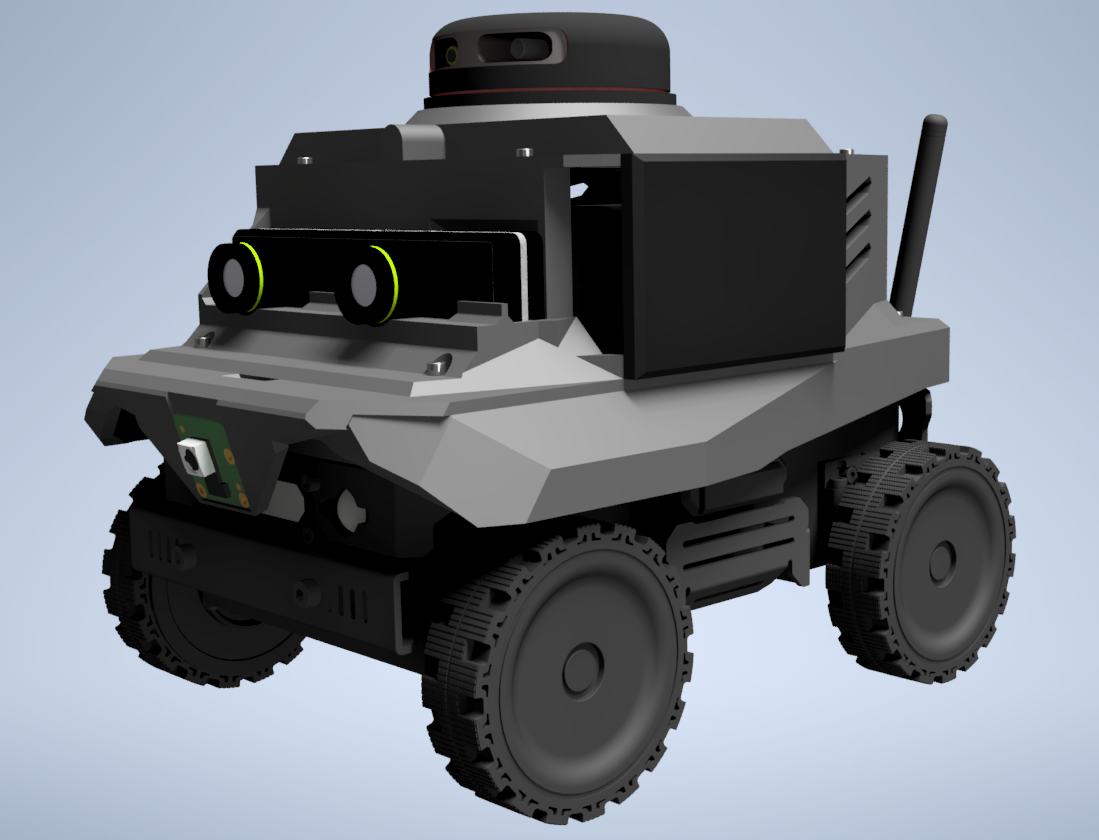
\includegraphics[width=0.48\textwidth]{fig_3_5_vehicle_cad.png}
  \caption[Photograph of the 1:14 RC vehicle instrumented with the camera and IMU.]{The 1:14 RC vehicle instrumented with camera, IMU, encoder and SBC, with each component labelled.}\label{fig:3.5}
\end{figure}

\subsection{Measurement instrumentation}
\label{sec:C.1.5}

The main tool for collecting evidence is the Logger Node of the ROS2 architecture, already described in adaptation A3 (\S\ref{sec:3.4.3}). The Logger Node records everything relevant that passes through the bus (observations, \emph{policy} actions, cage decisions, interventions, vehicle states) with timestamps, so that it can be reconstructed later.

The concrete metrics calculated from the logs are formally defined in Chapter~\ref{ch:04} and grouped into five families: \mbox{M-P} (performance: tracking error, trajectory completeness), \mbox{M-S} (safety: cage intervention rate, number of violations per SR), \mbox{M-I} (integration: latencies, jitter, throughput), \mbox{M-C} (behaviour: lateral stability, control smoothness) and \mbox{M-T} (transfer: difference between simulation and reality for each of the previous metrics, and metrics specific to the A5 gap). The details are in Chapter~\ref{ch:04}.

For additional quantitative evaluation on the \emph{scenario library}, the composite QED metric~\cite{gao2021} is taken as inspiration. It is a composite metric calibrated against human raters for autonomous driving tasks. It cannot be adopted as it is, because QED was developed and calibrated on CARLA and this thesis uses Gazebo. The formula can be transferred, but the calibrated weights would have to be recalculated for the lane-following scenario in Gazebo to get a metric with the same meaning. \emph{Behavior Metrics}~\cite{paniego2024} is considered as a helper tool for quantitative evaluation, since it already works with two simulators, CARLA and Gazebo. The decision to adopt it as the project's official metric is postponed to Phase 4, when the trained \emph{policy} is available and it can be calibrated against the author's own judgement.

\subsection{Documentation, version control and reproducibility}
\label{sec:C.1.6}

All project artefacts (documents, code, templates, traceability matrix, validation scripts) live in a single Git repository, based on one idea: the repository \emph{is} the project. The deliberate choice is \emph{plain text first}: artefacts are written in Markdown with minimal extensions (citations in the format \texttt{[Surname (year)]}, LaTeX equations, SVG/PNG figures in their own folder), not in industrial MBSE tools such as Cameo or Capella.

This choice differs from the MBSE proposal of Sprockhoff et al.~\cite{sprockhoff2023} for systems with AI components, which argues for SysML and structured tools as the backbone of the life cycle. The difference is about \emph{adoption cost}: for an individual thesis without industrial licences, version-controlled text files give better value for money, and they do the same job for traceability (with \texttt{traceability\_\allowbreak{}matrix.\allowbreak{}csv} + \texttt{check\_\allowbreak{}traceability.\allowbreak{}py}) and consistency (with automated review on every commit). The decision is recorded in \texttt{DECISIONS.md} with its justification and with the assumption that applying the framework in a medium-sized industrial team would make a move to MBSE worthwhile.

\section{Relation to the standards}
\label{sec:C.2}

The adapted V-Model builds on the current state of the standards for AI system safety. This section places each adaptation within that landscape and separates what is consistent with each standard from what goes further. The review follows the order of publication, which roughly matches the order in which industry adopted them.

\subsection{ISO 26262:2018 — Functional Safety for Road Vehicles}
\label{sec:C.2.1}

ISO 26262:2018 applies the classical V-Model to the automotive industry. The thesis takes it as its starting point and as a framework whose general structure it aims to keep.

\begin{itemize}
  \item \textbf{Consistent:} the five-level structure L1–L5, the idea of a safety requirement, the principle of a two-way link between specification and V\&V, and the derivation of requirements from the HARA with assignment of ASIL levels.
  \item \textbf{Goes further:} ISO 26262 does not consider learned modules. Adaptations A1, A2 and A3 are explicit extensions that bring in RL components without breaking the general structure of the standard. The approach is additive \emph{tailoring}: nothing is removed, and only what is strictly needed is added.
\end{itemize}

\subsection{ISO 21448:2022 — SOTIF (Safety Of The Intended Functionality)}
\label{sec:C.2.2}

ISO 21448:2022 extends safety beyond faults, including the use of functions under unexpected conditions. It is the official response to the fact that systems with ML-based perception and decision making can behave wrongly without any component having \enquote{failed} in the classical sense~\cite{wang2024}.

\begin{itemize}
  \item \textbf{Consistent:} adaptation A5 (bounded operational validation and measurement of the sim-to-real gap) matches directly the SOTIF idea that static validation is not enough when the ODD is not fully specified. Adaptation A3 (continuous runtime monitoring) matches the SOTIF principle of managing \emph{triggering conditions} found during operation.
  \item \textbf{Goes further:} A3 proposes runtime monitoring as an explicit architectural level of the life cycle, not only as a recommended practice during operation.
\end{itemize}

\subsection{ISO/IEC TR 5469:2024 — AI Functional Safety}
\label{sec:C.2.3}

ISO/IEC TR 5469:2024 is so far the most specific standards document on the use of AI in safety functions. It contributes three things to the proposed framework: the classification of AI technology by usage level and by technology class (Class I, II and III; clause 6), the \emph{three-stage realization principle} (clause 7), and the properties and risk factors of AI systems (clause 8: level of automation and control, transparency and explainability, complexity of the environment and vague specifications, resilience to adversarial inputs, AI hardware, and maturity of the technology).

\begin{itemize}
  \item \textbf{Consistent:} the thesis's PPO \emph{policy} is at best a Class II element of TR 5469 (existing functional safety standards only cover part of its required properties, and complementary methods are needed), and adaptation A2 (statistical Policy Behavioral Evaluation) is one of those complementary methods. Required two-way traceability (A4) has no direct counterpart among the TR's properties; its anchor in the standards is argued in C.2.5 and C.2.6. The split into Cage Spec / Training Spec (A1) takes the distinction made by the \emph{three-stage realization principle} between data acquisition, knowledge induction and processing, and applies it to the design process, which the TR itself does not present as a life cycle.
  \item \textbf{Goes further:} explicitly separating the Cage Spec (a conventional element that, by analogy, matches Class I) and the Training Spec (meta-design for a Class II element) into separate version-controlled documents is a practical refinement of the TR, which the standard does not detail at that level.
\end{itemize}

\subsection{ISO/PAS 8800:2024 — Road Vehicles, Safety and AI}
\label{sec:C.2.4}

ISO/PAS 8800:2024 is the automotive document on safety and AI, closely linked to the general concepts of TR 5469. It extends ISO 26262 and ISO 21448 to AI elements: functional safety risks are handled by \emph{tailoring} the relevant clauses of ISO 26262 (Parts 4, 6 and 8), and functional insufficiencies by extending the SOTIF concepts. An example use case published by BSI for the UK CCAV~\cite{hawkins2025}, on an ML traffic-sign detector with stop-sign requirements, shows how ISO 26262, SOTIF and ISO/PAS 8800 are combined on an ML component.

\begin{itemize}
  \item \textbf{Consistent:} the additive \emph{tailoring} of the adapted V-Model matches that of ISO/PAS 8800. The five adaptations A1–A5 can reasonably be aligned with the areas the standard identifies as critical (definition of the operating environment, systematic analysis of insufficiencies, monitoring after deployment).
  \item \textbf{Goes further:} applying the framework to a complete case, from HARA to physical deployment and with an empirical measurement of the gap, is more concrete than the examples published so far.
\end{itemize}

\subsection{UL 4600 — Standard for Safety for the Evaluation of Autonomous Products}
\label{sec:C.2.5}

UL 4600~\cite{ul4600,koopman2023} focuses on the \emph{safety case} and on structured evidence as the main way to provide assurance for autonomous products.

\begin{itemize}
  \item \textbf{Consistent:} the Traceability Matrix H$\leftrightarrow$SR$\leftrightarrow$C$\leftrightarrow$SC$\leftrightarrow$M is a small safety case in the spirit of UL 4600: every safety \emph{claim} is backed by an explicit argument (the cage rule, the scenario, the metric) and by traceable evidence (the logs, the experimental results).
  \item \textbf{Goes further:} A4 turns traceability into a hard constraint enforced by an automated tool (\texttt{check\_\allowbreak{}traceability.\allowbreak{}py}), instead of a documentation practice that someone has to review.
\end{itemize}

\subsection{AMLAS — Assurance of Machine Learning for Autonomous Systems}
\label{sec:C.2.6}

AMLAS, consolidated by Paterson et al.~\cite{paterson2025}, is not a formal standard but a method with GSN (\emph{Goal Structuring Notation}) patterns for building safety arguments about ML components. It is being used as input to new standards, in particular ISO/PAS 8800.

\begin{itemize}
  \item \textbf{Consistent:} the claim-argument-evidence approach of AMLAS matches the two-way traceability proposed as A4. The data-centred life cycle that AMLAS sets out (requirements definition, data management, learning, verification, deployment, monitoring) broadly matches the project phases described in \S\ref{sec:3.5.3}.
  \item \textbf{Goes further:} AMLAS has mostly been tested on supervised models. The framework in this thesis is designed explicitly for RL \emph{policies}, an area that AMLAS still covers poorly.
\end{itemize}

\subsection{The simplified HARA and how it relates to the formal version of the standard}
\label{sec:C.2.7}

Clause 6 of Part 3 of ISO 26262:2018 defines the formal HARA method for automotive \emph{items}: situation analysis, systematic identification of the hazards linked to the item's functions, classification of each hazard along three axes (severity S, scale S0–S3; exposure E, scale E0–E4; controllability C, scale C0–C3) and derivation of the \emph{ASIL} (Automotive Safety Integrity Level, QM/A/B/C/D) through a table that combines S$\times$E$\times$C. The ASIL sets the level of rigour required for the rest of the life cycle, including design measures, verification techniques and test coverage.

The version used in this thesis is explicitly called a \emph{simplified HARA}, and is labelled that way in the header of the Hazard Register. There are three differences from the formal standard, stated here openly:

\begin{itemize}
  \item \textbf{The S/E/C scales are kept but reinterpreted for a scale vehicle.} The three scales keep the granularity of the standard (S1–S3, E1–E4, C1–C3), but the definitions of each level are adapted to a 1:14 scale vehicle on a closed track. S3 no longer means \enquote{fatal injury} but \enquote{total loss of the integrity of the platform}. E3 is defined as \enquote{10–50\,\% of the operating time} within the declared ODD (a banding specific to this project: in the standard's duration-based exposure classes, E3 corresponds to 1–10\,\% and E4 to more than 10\,\% of the average operating time). C2 keeps the meaning of \enquote{controllable in > 90\,\% of the cases}, but with respect to the rule-based cage instead of the human driver. This adapted rubric is versioned together with the register and can be audited.
\end{itemize}

\begin{itemize}
  \item \textbf{No formal ASIL is assigned; a qualitative \enquote{Criticality} is used instead.} For each hazard, the simplified HARA produces a qualitative criticality label with four levels (Low, Medium, Medium-High, High), obtained by combining S, E and C qualitatively, and used only to prioritise mitigation work. No ASIL letter is assigned because the ASIL is a legal and normative construct meant for industrial certification, not for the methodological demonstration that the thesis aims at. Giving a scale car an \enquote{ASIL B} would suggest a precision that is not there, which the framework prefers to avoid. The qualitative criticality is honest about what is measured and what it is used for. Separately, the Safety Requirements have their own criticality rubric with two classes, \mbox{SR-CL-A} and \mbox{SR-CL-B}, defined in \S\ref{sec:4.5.3} of Chapter~\ref{ch:04} and with different practical consequences (minimum rigour of implementation and verification).
\end{itemize}

\begin{itemize}
  \item \textbf{An STPA-light analysis is added for selected hazards.} The simplified HARA is complemented by an \emph{STPA-light} analysis applied to high-criticality hazards and limited to the four categories of \emph{unsafe control actions}: action not given when needed, given when it should not be, given with the wrong magnitude, and given at the wrong time. This adds systemic failure modes that a pure HARA, focused on consequences, tends to under-represent. Using STPA is a common methodological borrowing in recent safety practice for systems with AI components, and it is documented as such, not as part of the formal ISO 26262 HARA.
\end{itemize}

What the simplified HARA \emph{keeps} is what matters most in the method: the systematic listing of hazards based on the analysis of the item, their classification before requirements are derived, two-way traceability between each hazard and the SRs that mitigate it (adaptation A4), and an auditable record of every classification decision. The process structure (situation $\rightarrow$ hazards $\rightarrow$ classification $\rightarrow$ SRs) is the same as in the standard. What changes is the type of final output (qualitative criticality instead of ASIL) and the addition of STPA-light for the hazards with the highest relative severity.

The split of work with ISO 21448 (SOTIF) follows the usual division in industry. The simplified HARA identifies systematic failures of the system, which is the traditional focus of ISO 26262. The \emph{insufficiencies of the intended functionality}, meaning behaviour that is correct according to the specification but hazardous in operation, which is the focus of SOTIF, are covered by adaptation A5 (empirical measurement of the sim-to-real gap) and adaptation A3 (runtime monitoring over intervention logs), not by the HARA. This split is visible in the traceability matrix: the H$\leftrightarrow$SR links cover the ISO 26262 part of the problem, and the \enquote{expected evidence mode} column (test / statistical analysis / runtime) covers the SOTIF part where it applies.

\begin{figure}[!htbp]
  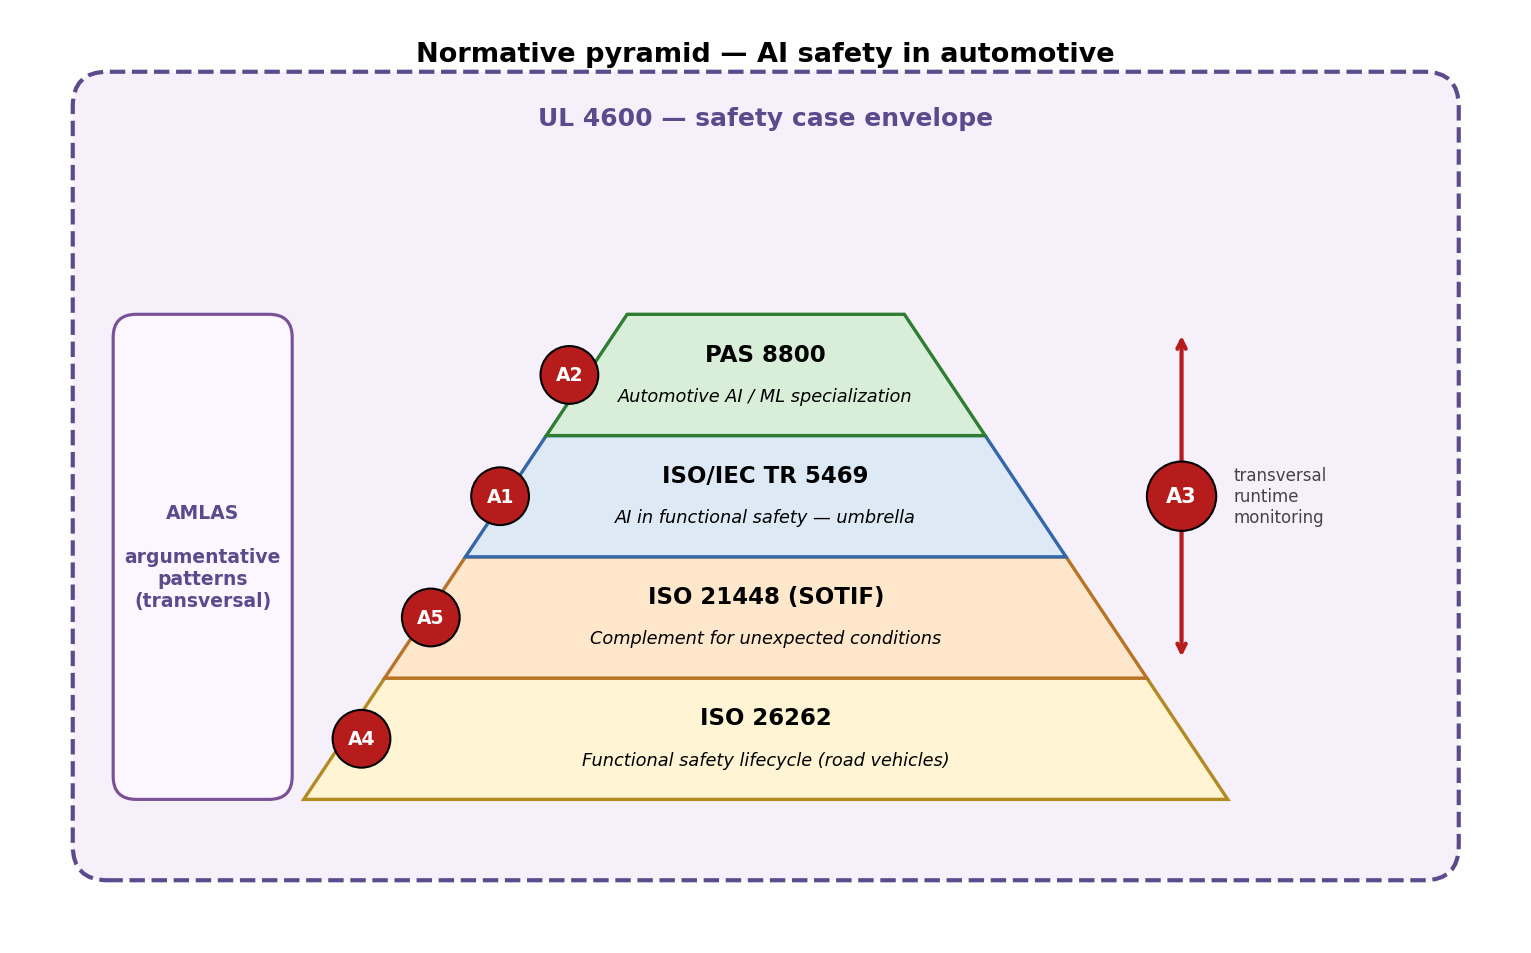
\includegraphics[width=0.80\textwidth]{fig_3_6_normative_pyramid.png}
  \caption[Diagram of the normative pyramid.]{Normative pyramid: ISO 26262 at the base as the life cycle, SOTIF as the complement for unexpected conditions, TR 5469 as the general AI layer, PAS 8800 as the automotive AI extension, UL 4600 as the safety case around everything, and AMLAS as argumentation patterns that apply across all of them. The five adaptations A1–A5 are marked on the pyramid with their scope of application.}\label{fig:3.6}
\end{figure}

% GENERATED by md2tex.py from ../draft_v5_en/back/D_appendix_odd.md -- do not edit by hand.
% Change the Markdown and run `python md2tex.py`; edits here are overwritten.

% NOTE: the source tables carry no header row; the headers below are supplied
% by md2tex.py (SUPPLIED_TABLE_HEADERS) from the column contents.

\chapter{Operational domain specification}
\label{app:D}

This is the full table of parameters for the four operational domains. Each parameter has a name, a value for each domain and a source. Whenever a named parameter exists, no claim about the domain in the main text relies on a qualitative description.

% layout: longtable, fixed, \footnotesize, 164 of 165 mm
\begingroup
\footnotesize\setlength{\tabcolsep}{4pt}
\setlength{\LTleft}{0pt}\setlength{\LTright}{\fill}\setlength{\LTcapwidth}{\textwidth}
\begin{longtable}{@{}>{\RaggedRight\arraybackslash}p{22.6mm}>{\RaggedRight\arraybackslash}p{29.3mm}>{\RaggedRight\arraybackslash}p{15.4mm}>{\RaggedRight\arraybackslash}p{11.2mm}>{\RaggedRight\arraybackslash}p{11.9mm}>{\RaggedRight\arraybackslash}p{11.9mm}>{\RaggedRight\arraybackslash}p{44.3mm}@{}}
\caption{Parameters of the four operational domains.}\label{tab:D.1} \\
  \toprule
  \tabhead{Parameter} & \tabhead{Meaning} & \tabhead{\mbox{ODD-1}} & \tabhead{\mbox{ODD-2}} & \tabhead{\mbox{ODD-3}} & \tabhead{\mbox{ODD-4}} & \tabhead{Source} \\
  \midrule
  \endfirsthead
  \multicolumn{7}{@{}l}{\emph{(continued)}} \\
  \toprule
  \tabhead{Parameter} & \tabhead{Meaning} & \tabhead{\mbox{ODD-1}} & \tabhead{\mbox{ODD-2}} & \tabhead{\mbox{ODD-3}} & \tabhead{\mbox{ODD-4}} & \tabhead{Source} \\
  \midrule
  \endhead
  \midrule
  \multicolumn{7}{r@{}}{\emph{(continued on next page)}} \\
  \endfoot
  \bottomrule
  \endlastfoot
  \texttt{*.V\_MAX} / \texttt{*.V\_MAX\_STRAIGHT} & Speed ceiling, straight (m/s) & 0.5 & 0.5 & 0.5 & 0.5 & \sr{004}; \cagerule{04}. Operating point = 0.20 \\
  \addlinespace[2pt]
  \texttt{*.V\_MAX\_CURVE} & Speed ceiling, curve (m/s) & n/a & n/a & 0.25 & 0.25 & \sr{004}; \cagerule{04} \\
  \addlinespace[2pt]
  \texttt{*.K\_KAPPA} & Curvature speed-decay coeff. & n/a & n/a & 0.3 & 0.3 & \sr{004}; \cagerule{04} \\
  \addlinespace[2pt]
  \texttt{*.KAPPA\_MAX} & Max local curvature (1/m) & 0 & 0 & 1.14 & 1.14 & 1 / 0.876 m (complex\_b centre R\_min); driven $\approx$ 1.00; oval legacy 1.25 \\
  \addlinespace[2pt]
  \texttt{*.A\_LAT\_MAX} & Max commanded lateral accel. (m/s\textsuperscript{2}) & 9.81 & 9.81 & \mbox{TBD-Q10} & \mbox{TBD-Q10} & Coulomb ceiling FRICTION$\times$g (\mbox{ODD-1}); \mbox{ODD-3} deferred to \mbox{M-4} \\
  \addlinespace[2pt]
  \texttt{*.T\_CTRL} & Control cycle period (ms) & 50 & 50 & 50 & 50 & cage.yaml (20 Hz deployment); sim train/eval 10 Hz (control\_dt 0.10 s) \\
  \addlinespace[2pt]
  \texttt{*.\allowbreak{}LATENCY\_\allowbreak{}NOMINAL} & Nominal control latency (ms) & 50 & 50 & 50 & 50 & Implementation; \sr{001} rationale \\
  \addlinespace[2pt]
  \texttt{*.STALENESS\_MAX} & Max admissible state staleness (ms) & 200 & 200 & 200 & 200 & \sr{007} (cage budget 0.5 s at 10 Hz, cage 0.6.1) \\
  \addlinespace[2pt]
  \texttt{*.LANE\_EDGE} & Geometric lane edge (m, from centre) & 0.1225 & 0.1225 & 0.1225 & 0.1225 & LANE\_WIDTH / 2 \\
  \addlinespace[2pt]
  \texttt{*.CORRIDOR\_EDGE} & Episode-termination edge (m) & 0.1225 & 0.1225 & 0.1225 & 0.1225 & Episode-termination logic (= LANE\_EDGE) \\
  \addlinespace[2pt]
  \texttt{*.ROAD\_EDGE} & Painted road boundary (m, from centre) & 0.26 & 0.26 & 0.26 & 0.26 & ROAD\_WIDTH / 2; off-road / \met{S5} criterion (oval legacy 0.25) \\
  \addlinespace[2pt]
  \texttt{*.STUCK\_TIMEOUT} & Stuck criterion timeout (s) & n/a & n/a & n/a & n/a & Subsumed by env truncation (500 $\times$ 0.10 s = 50 s); \mbox{TBD-Q11} \\
  \addlinespace[2pt]
  \texttt{*.OBS\_DIM} & Observation & camera 84$\times$84$\times$4 (policy); CV lane-estimate (cage) & same & same & same & Track \enquote*{E} (\dec{43}). F-track baseline: 6-D state vector \\
  \addlinespace[2pt]
  \texttt{*.ACT\_DIM} & GE4-realised action vector dimension & 1 & 1 & 1 & 1 & Steering-only verdict parameter (\dec{49}). Posterior Gazebo and Isaac configs set 2 locally (\dec{50}/\allowbreak{}\dec{59}/\allowbreak{}\dec{60}) without changing this ODD value \\
\end{longtable}
\endgroup

\section{Open questions of the domain and their closure}
\label{sec:D.1}

Of the twelve quantitative questions that were opened when the specification was written, eleven are closed with an explicit value and a date. The twelfth is still open because it depends on hardware, not because it was forgotten.

% layout: longtable, fixed, \footnotesize, 164 of 165 mm
\begingroup
\footnotesize\setlength{\tabcolsep}{4pt}
\setlength{\LTleft}{0pt}\setlength{\LTright}{\fill}\setlength{\LTcapwidth}{\textwidth}
\begin{longtable}{@{}>{\RaggedRight\arraybackslash}p{11.9mm}>{\RaggedRight\arraybackslash}p{25.7mm}>{\RaggedRight\arraybackslash}p{9.7mm}>{\RaggedRight\arraybackslash}p{12.1mm}>{\RaggedRight\arraybackslash}p{92.9mm}@{}}
\caption{Open quantitative questions of the domain and their closure.}\label{tab:D.2} \\
  \toprule
  \tabhead{ID} & \tabhead{Question} & \tabhead{Owner} & \tabhead{Status} & \tabhead{Resolution} \\
  \midrule
  \endfirsthead
  \multicolumn{5}{@{}l}{\emph{(continued)}} \\
  \toprule
  \tabhead{ID} & \tabhead{Question} & \tabhead{Owner} & \tabhead{Status} & \tabhead{Resolution} \\
  \midrule
  \endhead
  \midrule
  \multicolumn{5}{r@{}}{\emph{(continued on next page)}} \\
  \endfoot
  \bottomrule
  \endlastfoot
  \mbox{TBD-Q1} & Friction coefficient of the road surface? & SS & closed & 1.0 — world SDFs ship an empty \texttt{<surface><friction>} block; Gazebo ODE defaults \texttt{mu1=mu2=1.0}. Inferred, not explicit \texttt{<mu>}; re-read if a future world sets one. (2026-05-14) \\
  \addlinespace[2pt]
  \mbox{TBD-Q2} & Max commanded lateral accel., \mbox{ODD-1}? & SS & closed & 9.81 — Coulomb ceiling FRICTION$\times$g. Physical envelope, not a typical value (operational \texttt{a\_lat ≈ 0} at $\kappa$=0). (2026-05-14) \\
  \addlinespace[2pt]
  \mbox{TBD-Q3} & Numerical drivable-corridor edge; why differ from LANE\_EDGE? & SS & closed & 0.1225 — the env terminates at \texttt{|ey| > lane\_width/2}; CORRIDOR\_EDGE = LANE\_EDGE, no separate margin. (Track \enquote*{E} adds off-road-by-road-centre-distance vs ROAD\_EDGE = 0.26 for self-approaching loops, docs/11 \S\ref{sec:3.5}.) (2026-05-14) \\
  \addlinespace[2pt]
  \mbox{TBD-Q4} & Lighting-degradation + noise in the nominal-adverse profile? & SS & closed & Superseded on track \enquote*{E} by the camera visual-degradation stressors (\S\ref{sec:5.5}): glare/low-light/motion-blur (\hz{10}), levels grounded in the GE2 oracle. F-track legacy value in \texttt{adverse\_\allowbreak{}profiles.\allowbreak{}yaml}. (2026-06-03; retargeted 2026-07-07) \\
  \addlinespace[2pt]
  \mbox{TBD-Q5} & Latency / jitter / actuation-imperfection profile? & SS & closed & Superseded on track \enquote*{E} — the perception channel, not state-vector latency, is the \mbox{ODD-2} axis; F-track legacy \texttt{odd2\_\allowbreak{}adverse\_\allowbreak{}with\_\allowbreak{}latency} retained historically. (2026-06-03; retargeted 2026-07-07) \\
  \addlinespace[2pt]
  \mbox{TBD-Q6} & Obstacle geometry / position / quantity? & SS & closed (retired) & Retired — no obstacle observation channel; no obstacle scenario in the verdict library. The F4 spec-only box profile is withdrawn. (2026-07-07) \\
  \addlinespace[2pt]
  \mbox{TBD-Q7} & Full parameterisation of the adverse-full profile? & SS & closed & On track \enquote*{E} = the union/compound of the \S\ref{sec:5.5} camera stressors (e.g. \scn{PERT-13} = worn markings + glare). (2026-06-03; retargeted 2026-07-07) \\
  \addlinespace[2pt]
  \mbox{TBD-Q8} & Total loop length of the curvy world? & SS & closed & complex\_b: 19.22 m (centre) / 19.93 m (driven), from \texttt{complex\_\allowbreak{}b\_\allowbreak{}centerline.\allowbreak{}yaml} (\texttt{perimeter\_m}). Oval legacy $\approx$ 8.0232 m (centre) / 8.79 m (driven). (2026-05-21; retargeted 2026-07-07) \\
  \addlinespace[2pt]
  \mbox{TBD-Q9} & Minimum curvature radius / KAPPA\_MAX? & SS & closed & complex\_b: R\_min $\approx$ 0.876 m (centre) / 0.998 m (driven) $\rightarrow$ KAPPA\_MAX $\approx$ 1.14 m\textsuperscript{$-1$} (centre) / 1.00 (driven); shaped to the \S\ref{sec:6.2} monocular boundary. Oval legacy R\_min 0.80 $\rightarrow$ 1.25 m\textsuperscript{$-1$}. (2026-05-21; retargeted 2026-07-07) \\
  \addlinespace[2pt]
  \mbox{TBD-Q10} & Max commanded lateral accel., \mbox{ODD-3}, from FRICTION + V\_MAX\_CURVE? & SS & \mbox{M-4} (F5) & OPEN, and now closed \emph{as} open (Phase 5 ended 01.09.2026 without \mbox{M-4}, and no further physical measurement is planned). Coulomb upper bound \texttt{A\_LAT\_MAX ≤ FRICTION×g = 9.81 m/s²}; operational value at V\_MAX\_CURVE=0.25 on driven R\_min$\approx$1.0 m is \texttt{V²/R ≈ 0.063 m/s²} — well below. The 2-D verdict-of-record campaign ran at $\approx$0.216 m/s (\texttt{a\_lat ≈ 0.047 m/s²}), so it neither approaches nor could bound the envelope: in Gazebo \texttt{A\_LAT\_MAX} is a \emph{property of the friction model that was assumed}, so measuring it there would return the assumption. Unmeasurable in simulation by construction (\dec{33}) — a hardware dependency, not an outstanding action item — and the hardware phase closed without taking it. The figure would close with \textbf{\mbox{M-4}}; it is carried as future work, and this spec stays below v1.0 by design. \\
  \addlinespace[2pt]
  \mbox{TBD-Q11} & Stuck-criterion timeout? & SS & closed & n/a — no separate stuck monitor; env truncation \texttt{max\_\allowbreak{}episode\_\allowbreak{}steps × control\_dt = 500 × 0.10 s = 50 s} is the implicit timeout. (2026-05-21, F3 update 2026-06-01) \\
  \addlinespace[2pt]
  \mbox{TBD-Q12} & Do \mbox{ODD-4} profiles add any stressor beyond \mbox{ODD-2}? & SS & closed & No — \mbox{ODD-4} = \mbox{ODD-3} geometry $\times$ \mbox{ODD-2} perception stressors (\S\ref{sec:7.1}), realised as curve-traversing complex\_b scenarios (\scn{PERT-11}/\allowbreak{}12/13, \scn{FRONT-07}). (2026-06-03; retargeted 2026-07-07) \\
\end{longtable}
\endgroup

% GENERATED by md2tex.py from ../draft_v5_en/back/E_appendix_cage.md -- do not edit by hand.
% Change the Markdown and run `python md2tex.py`; edits here are overwritten.

\chapter{Cage parameters}
\label{app:E}

This appendix reproduces the full version-controlled parameter file, exactly as the node reads it at runtime. Every experimental run stores the cryptographic identifier of this file together with the other reproducibility metadata, so any result in Chapter~\ref{ch:08} is clearly linked to the exact configuration that produced it.

The values marked as provisional are waiting to be calibrated on the physical platform. The process to close them is defined: measure, update the file, increase the version, run the verification suite and the affected scenarios again, and record the change in the change log.

\begingroup
\footnotesize
\begin{verbatim}
# =============================================================
# Safety Cage Configuration
# -------------------------------------------------------------
# This file is the single source of truth for all cage parameters.
# It is referenced by hash in the metadata of every experimental run.
#
# Update procedure:
# 1. Edit this file.
# 2. Add an entry to docs/08_change_log.md with rationale and evidence.
# 3. Run pytest cage/tests/ to verify all unit tests still pass.
# 4. Re-run affected scenarios.
# 5. Update docs/04_cage_specification.md if any logic changed.
# =============================================================
cage:
  version: "0.6.1"
  compatible_sr_spec_version: "1.0"
  description: "0.6.1 (2026-06-10, track 'E')"
  # -----------------------------------------------------------
  # Operating mode
  # -----------------------------------------------------------
  # "enforcement" applies corrections; "monitoring" only logs them.
  default_mode: "enforcement"
  # -----------------------------------------------------------
  # Control loop
  # -----------------------------------------------------------
  control:
    cycle_period_ms: 50         # 20 Hz control loop
    staleness_max_ms: 200       # SR-007: max age of state observation
  # -----------------------------------------------------------
  # Inter-cycle oscillation detection (SR-010 Part 2)
  # -----------------------------------------------------------
  # The cage_node tracks the sign of each steering-affecting rule's
  # correction (C-01, C-02, C-03) across cycles. When the alternation
  # rate of a rule exceeds f_osc_max_hz in a t_osc_window_s sliding
  # window, the cycle is logged for offline review. When the violation
  # persists for more than t_osc_persist_s, the cage_node sets
  # ctx["oscillation_detected"] = True and C-05 fires its
  # "oscillation_detected" trigger to enter emergency mode. Defaults
  # mirror SR-010 §"Inter-cycle oscillation check".
  oscillation:
    f_osc_max_hz: 5.0          # alternation-rate threshold
    t_osc_window_s: 1.0        # sliding-window length
    t_osc_persist_s: 3.0       # sustained-violation duration → emergency
  # -----------------------------------------------------------
  # State validity ranges (SR-007)
  # -----------------------------------------------------------
  state_validity_ranges:
    lateral_offset_m: [-0.30, 0.30]      # broader than d_max to detect outliers
    heading_error_rad: [-1.57, 1.57]     # ±π/2; beyond, state is implausible
    speed_mps: [-0.10, 1.50]             # negative for sensor noise tolerance
  n_missing_max_cycles: 5                # SR-007: missing state cycles
  # -----------------------------------------------------------
  # Rule C-01 — Lane boundary hard limit (SR-001, H-01)
  # -----------------------------------------------------------
  # Rationale: SR-001 §Parameters traces d_max to
  #   ODD-1.ROAD_WIDTH/2 - Δ = 0.25 - 0.09 = 0.16 m
  # where Δ aggregates LiDAR lateral noise (~0.01 m, [provisional, M-1]),
  # one-cycle drift v_max·LATENCY_NOMINAL = 0.025 m ([provisional, M-2]),
  # and CobraFlex 1:14 half-footprint (~0.05 m).
  c01_lane_boundary:
    enabled: true
    d_max_m: 0.16              # SR-001 threshold [provisional, M-1, M-2]
    h_d_m: 0.02                # hysteresis margin
    correction_gain: 1.5       # how aggressively to correct toward centre
  # -----------------------------------------------------------
  # Rule C-02 — Heading error limit (SR-002, H-02)
  # -----------------------------------------------------------
  # Rationale: SR-002 §Parameters derives θ_max from a bicycle-model
  # recoverability calculation; the chosen value falls inside the
  # recoverable envelope with factor ~2 margin.
  c02_heading_limit:
    enabled: true
    theta_max_rad: 0.4363      # 25 deg, SR-002
    h_theta_rad: 0.0349        # 2 deg hysteresis
    correction_gain: 1.0
  # -----------------------------------------------------------
  # Rule C-03 — Predictive lane departure / TTLC (SR-003, H-01/H-02)
  # -----------------------------------------------------------
  # Rationale: SR-003 §Parameters decomposes t_min into 0.3 s cage-side
  # margin (defensible by kinematics) + 0.7 s policy-side margin
  # ([provisional, F3 post-prototype]).
  c03_ttlc:
    enabled: true
    t_min_s: 1.0               # SR-003; policy-side component provisional
    horizon_s: 3.0             # max projection horizon for TTLC computation
    urgency_gain_max: 2.0      # max steering bias when ttlc -> 0
    d_max_m: 0.16              # must mirror c01_lane_boundary.d_max_m
    v_min_estimate_mps: 0.05   # speeds below this -> TTLC = inf (avoid div-by-zero)
  # -----------------------------------------------------------
  # Rule C-04 — Speed ceiling (SR-004, H-03)
  # -----------------------------------------------------------
  # Rationale: SR-004 §Parameters. v_max_straight mirrors ODD-1.V_MAX;
  # v_max_curve reflects the kinematic envelope at KAPPA_MAX (TBD-Q9 in
  # ODD-Spec) under FRICTION (TBD-Q1). The interpolation coefficient
  # k_kappa is set so the linear interpolation crosses v_max_curve at
  # the working assumption for KAPPA_MAX on `odd3_curvy_loop`.
  c04_speed_ceiling:
    enabled: true
    v_max_straight_mps: 0.5            # [provisional, M-4 + ODD TBD-Q1]
    v_max_curve_mps: 0.25              # [provisional, M-4 + ODD TBD-Q9]
    curvature_threshold_inv_m: 0.05    # |kappa| above this is "curve"
    k_kappa_mps_per_curvature: 0.3     # [provisional, tightens with KAPPA_MAX]
    curvature_estimation_window_s: 0.5  # window for kappa estimation
    k_throttle_per_mps: 5.0            # proportional throttle reduction per m/s excess
  # -----------------------------------------------------------
  # Rule C-05 — Emergency mode (SR-005, SR-007, SR-008; H-04, H-06, H-07)
  # -----------------------------------------------------------
  # Rationale:
  # - theta_warning < theta_max (SR-002): early-warning band ~5 deg.
  # - d_warning   < d_max     (SR-001): early-warning band 0.04 m.
  # - delta_t_max = 4 control cycles: STPA-informed persistence
  #   requirement to ignore single-cycle glitches; instantaneous
  #   triggers would produce spurious activations under benign noise.
  # - a_min: the kinematic stopping time at v_max_straight = 0.5 m/s is
  #   0.5 / a_min = 1.67 s, consistent with SR-008 t_stop_max = 1.7 s.
  #   If M-3 demonstrates higher achievable deceleration, a_min may be
  #   raised in a coordinated SR-005 / SR-008 revision (next bump).
  # - require_explicit_reset: STPA-informed asymmetric exit to prevent
  #   oscillation between modes near the trigger boundary.
  c05_emergency:
    enabled: true
    # Compound-state trigger — low-energy variant (SR-005 Trigger A)
    theta_warning_rad: 0.3491   # 20 deg
    d_warning_m: 0.12
    delta_t_max_s: 0.2          # 4 cycles; STPA-informed persistence
    # Compound-state trigger — high-energy variant (SR-005 Trigger B)
    # When |v| > v_warning_mps the same compound condition triggers after
    # the shorter delta_t_max_fast_s because the kinematic margin at
    # elevated speed leaves less time to absorb the excursion.
    v_warning_mps: 0.4          # 80% of v_max_straight (0.5 mps)
    delta_t_max_fast_s: 0.1     # 2 cycles; shorter persistence at high energy
    # Emergency response
    a_min_mps2: 0.3             # [provisional, M-3]; consistent with SR-008
    freeze_steering: true       # steering stays at value at activation
    # Reset policy
    require_explicit_reset: true   # must receive reset signal AND condition cleared
    # Trigger 3 — stale-state budget (SR-007). Aligned with Trigger 5's
    # missing-state budget at the 10 Hz sim control rate:
    # n_missing_max_cycles (5) × control_dt (0.1 s). See 0.6.1 note above.
    staleness_max_s: 0.5
    # Trigger 8 — perception invalid (track 'E'; SR-013/SR-014; D-43).
    # When true, ctx["perception_invalid"] (set by the external CV
    # lane-estimator supervisor) fires the C-05 controlled stop. The
    # supervisor's thresholds live with the supervisor; the cage only
    # consumes the boolean. Code default is false (inert pre-0.6.0).
    perception_trigger_enabled: true
  # -----------------------------------------------------------
  # Rule C-06 — Actuator rate limiter (SR-006, H-05)
  # -----------------------------------------------------------
  # Rationale: SR-006 §Parameters declares both deltas as conservative
  # defaults. Final calibration requires (i) actuator envelope from M-5,
  # and (ii) cross-check against 95th-percentile delta of the policy's
  # natural action distribution after F3 prototype.
  c06_rate_limiter:
    enabled: true
    delta_max_steering_per_cycle: 0.15      # [provisional, M-5 + F3 prototype]
    delta_max_throttle_per_cycle: 0.10      # [provisional, M-5 + F3 prototype]
  # -----------------------------------------------------------
  # Logging configuration
  # -----------------------------------------------------------
  logging:
    cage_status_topic: "/cage_status"
    log_every_cycle: true                   # log even when no rule fires
    include_state_in_log: true              # include full state in /cage_status
    include_action_delta: true              # include delta(safe, raw) in log
  # -----------------------------------------------------------
  # Topic configuration (ROS2)
  # -----------------------------------------------------------
  topics:
    raw_action_in: "/raw_action"
    state_obs_in: "/state_obs"
    external_stop_in: "/external_stop"
    safe_action_out: "/safe_action"
    cage_status_out: "/cage_status"
    emergency_signal_out: "/emergency"
    reset_in: "/cage_reset"
\end{verbatim}
\endgroup

% GENERATED by md2tex.py from ../draft_v5_en/back/F_appendix_traceability.md -- do not edit by hand.
% Change the Markdown and run `python md2tex.py`; edits here are overwritten.

\chapter{Traceability matrix}
\label{app:F}

The matrix exists in two forms that are kept in sync. One is readable and organised by mitigation chain. The other can be processed by a machine, and the checker uses it to verify the eight coverage constraints. If any of them is broken, the corresponding review gate is blocked.

\section{Summary by mitigation chain}
\label{sec:F.1}

% layout: table, fixed, \footnotesize, 164 of 165 mm
\begin{table}[!htbp]
\caption{Traceability by mitigation chain, with the simulation verdict.}\label{tab:F.1}
\footnotesize\setlength{\tabcolsep}{4pt}
\begin{tabular}{@{}>{\RaggedRight\arraybackslash}p{12.9mm}>{\RaggedRight\arraybackslash}p{19.3mm}>{\RaggedRight\arraybackslash}p{31.8mm}>{\RaggedRight\arraybackslash}p{46.0mm}>{\RaggedRight\arraybackslash}p{20.1mm}>{\RaggedRight\arraybackslash}p{19.4mm}@{}}
  \toprule
  \tabhead{Hazard} & \tabhead{Safety Requirement} & \tabhead{Cage Rule(s)} & \tabhead{Scenarios} & \tabhead{Verifying Metric(s)} & \tabhead{Verdict (Sim)} \\
  \midrule
  \hz{01} & \sr{001} & \cagerule{01} & \scn{NOM-01}, \scn{NOM-02}, \scn{EDGE-02} & \met{S1} & Satisfied \\
  \addlinespace[2pt]
  \hz{01}, \hz{02} & \sr{003} & \cagerule{03} & \scn{NOM-02}, \scn{EDGE-01} & \met{S4} & Satisfied \\
  \addlinespace[2pt]
  \hz{02} & \sr{002} & \cagerule{02} & \scn{EDGE-01}, \scn{EDGE-04} & \met{P4} & Satisfied \\
  \addlinespace[2pt]
  \hz{02} & \sr{011} & \cagerule{06} + training & \scn{EDGE-01}, \scn{EDGE-04} & \met{P7} & Satisfied \\
  \addlinespace[2pt]
  \hz{03} & \sr{004} & \cagerule{04} & \scn{NOM-02}, \scn{EDGE-03} & \met{P3} & Satisfied \\
  \addlinespace[2pt]
  \hz{04}, \hz{07} & \sr{005} & \cagerule{05} & \scn{EDGE-04} & \met{S3} & Satisfied \\
  \addlinespace[2pt]
  \hz{05} & \sr{006} & \cagerule{06} & All scenarios & \met{I5} & Satisfied \\
  \addlinespace[2pt]
  \hz{06} & \sr{007} & \cagerule{05} (state-validity triggers) & \scn{PERT-02} & \met{S3} & Satisfied \\
  \addlinespace[2pt]
  \hz{07} & \sr{008} & \cagerule{05} (external-stop trigger) & \scn{NOM-03}, \scn{EDGE-04} & \met{S3} & Satisfied \\
  \addlinespace[2pt]
  \hz{08} & \sr{009} & training & \scn{NOM-01}, \scn{NOM-02}, \scn{NOM-03}, \scn{PERT-03} & \met{P6}, \met{S2} (monitoring) & Satisfied \\
  \addlinespace[2pt]
  \hz{09} & \sr{010} & arbiter & \scn{EDGE-04}, \scn{EDGE-05} & \met{S2}, \met{I3} & Not satisfied \\
  \addlinespace[2pt]
  \hz{10} & \sr{012} & \cagerule{01}, \cagerule{02}, \cagerule{03} (over CV state) + training & \scn{NOM-01}, \scn{PERT-04}, \scn{PERT-05}, \scn{PERT-06}, \scn{PERT-09}, \scn{PERT-10}, \scn{PERT-11}, \scn{PERT-12}, \scn{PERT-13} & \met{S1}, \met{S2} & Satisfied \\
  \addlinespace[2pt]
  \hz{11} & \sr{013} & \cagerule{05} (CV-estimator health $\rightarrow$ controlled stop) & \scn{NOM-01}, \scn{PERT-07}, \scn{PERT-13} & \met{S3} & Satisfied \\
  \addlinespace[2pt]
  \hz{12} & \sr{014} & \cagerule{05} (plausibility check $\rightarrow$ controlled stop) & \scn{NOM-01}, \scn{PERT-08}, \scn{PERT-04}..06, \scn{PERT-09}..10, \scn{PERT-11}..13 & \met{S1}, \met{S3} & Satisfied \\
  \bottomrule
\end{tabular}
\end{table}

\section{Machine-processable form}
\label{sec:F.2}

Each row is a chain from a hazard to a metric. A hazard appears in several rows because it covers several chains. The physical verdict column is marked not executed in every row: the deployment chain is built and has driven on hardware, but no run has been done under the scenario protocol (\S\ref{sec:10.4}d–\allowbreak{}e).

% layout: longtable, natural, \small, 146 of 165 mm
\begingroup
\small\setlength{\tabcolsep}{4pt}
\setlength{\LTleft}{0pt}\setlength{\LTright}{\fill}\setlength{\LTcapwidth}{\textwidth}
\begin{longtable}{@{}llllllll@{}}
\caption{Machine-processable form of the traceability matrix.}\label{tab:F.2} \\
  \toprule
  \rotatebox{90}{\tabhead{Hazard}} & \rotatebox{90}{\tabhead{Requirement}} & \tabhead{Rule} & \tabhead{Type} & \tabhead{Scenario} & \rotatebox{90}{\tabhead{Metric}} & \tabhead{Sim. verdict} & \tabhead{Phys. verdict} \\
  \midrule
  \endfirsthead
  \multicolumn{8}{@{}l}{\emph{(continued)}} \\
  \toprule
  \rotatebox{90}{\tabhead{Hazard}} & \rotatebox{90}{\tabhead{Requirement}} & \tabhead{Rule} & \tabhead{Type} & \tabhead{Scenario} & \rotatebox{90}{\tabhead{Metric}} & \tabhead{Sim. verdict} & \tabhead{Phys. verdict} \\
  \midrule
  \endhead
  \midrule
  \multicolumn{8}{r@{}}{\emph{(continued on next page)}} \\
  \endfoot
  \bottomrule
  \endlastfoot
  \hz{01} & \sr{001} & \cagerule{01} & cage rule & \scn{NOM-01} & \met{S1} & satisfied & not executed \\
  \hz{01} & \sr{001} & \cagerule{01} & cage rule & \scn{NOM-02} & \met{S1} & satisfied & not executed \\
  \hz{01} & \sr{001} & \cagerule{01} & cage rule & \scn{EDGE-02} & \met{S1} & satisfied & not executed \\
  \hz{01} & \sr{001} & \cagerule{01} & cage rule & \scn{NOM-01} & \met{S2} & satisfied & not executed \\
  \hz{01} & \sr{003} & \cagerule{03} & cage rule & \scn{NOM-02} & \met{S4} & satisfied & not executed \\
  \hz{01} & \sr{003} & \cagerule{03} & cage rule & \scn{EDGE-01} & \met{S4} & satisfied & not executed \\
  \hz{02} & \sr{002} & \cagerule{02} & cage rule & \scn{EDGE-01} & \met{P4} & satisfied & not executed \\
  \hz{02} & \sr{002} & \cagerule{02} & cage rule & \scn{EDGE-04} & \met{P4} & satisfied & not executed \\
  \hz{02} & \sr{003} & \cagerule{03} & cage rule & \scn{EDGE-01} & \met{S4} & satisfied & not executed \\
  \hz{03} & \sr{004} & \cagerule{04} & cage rule & \scn{NOM-02} & \met{P3} & satisfied & not executed \\
  \hz{03} & \sr{004} & \cagerule{04} & cage rule & \scn{EDGE-03} & \met{P3} & satisfied & not executed \\
  \hz{04} & \sr{005} & \cagerule{05} & cage rule & \scn{EDGE-04} & \met{S3} & satisfied & not executed \\
  \hz{05} & \sr{006} & \cagerule{06} & cage rule & \scn{NOM-01} & \met{I5} & satisfied & not executed \\
  \hz{05} & \sr{006} & \cagerule{06} & cage rule & \scn{NOM-02} & \met{I5} & satisfied & not executed \\
  \hz{06} & \sr{007} & \cagerule{05} & cage rule & \scn{PERT-02} & \met{S3} & satisfied & not executed \\
  \hz{07} & \sr{005} & \cagerule{05} & cage rule & \scn{EDGE-04} & \met{S3} & satisfied & not executed \\
  \hz{07} & \sr{008} & \cagerule{05} & cage rule & \scn{NOM-03} & \met{S3} & satisfied & not executed \\
  \hz{07} & \sr{008} & \cagerule{05} & cage rule & \scn{EDGE-04} & \met{S3} & satisfied & not executed \\
  \hz{10} & \sr{012} & \cagerule{01} & cage rule & \scn{PERT-04} & \met{S1} & satisfied & not executed \\
  \hz{10} & \sr{012} & \cagerule{02} & cage rule & \scn{PERT-05} & \met{S1} & satisfied & not executed \\
  \hz{10} & \sr{012} & \cagerule{03} & cage rule & \scn{PERT-06} & \met{S2} & satisfied & not executed \\
  \hz{10} & \sr{012} & — & training & \scn{PERT-04} & \met{S2} & satisfied & not executed \\
  \hz{10} & \sr{012} & \cagerule{01} & cage rule & \scn{PERT-09} & \met{S1} & satisfied & not executed \\
  \hz{10} & \sr{012} & \cagerule{01} & cage rule & \scn{PERT-10} & \met{S1} & satisfied & not executed \\
  \hz{11} & \sr{013} & \cagerule{05} & cage rule & \scn{PERT-07} & \met{S3} & satisfied & not executed \\
  \hz{12} & \sr{014} & \cagerule{05} & cage rule & \scn{PERT-08} & \met{S1} & satisfied & not executed \\
  \hz{12} & \sr{014} & \cagerule{05} & cage rule & \scn{PERT-08} & \met{S3} & satisfied & not executed \\
  \hz{12} & \sr{014} & \cagerule{05} & cage rule & \scn{PERT-09} & \met{S3} & satisfied & not executed \\
  \hz{12} & \sr{014} & \cagerule{05} & cage rule & \scn{PERT-10} & \met{S3} & satisfied & not executed \\
  \hz{08} & \sr{009} & — & training constraint & \scn{NOM-01} & \met{P6} & satisfied & not executed \\
  \hz{08} & \sr{009} & — & training constraint & \scn{PERT-03} & \met{P6} & satisfied & not executed \\
  \hz{09} & \sr{010} & — & arbiter & \scn{EDGE-04} & \met{I3} & satisfied & not executed \\
  \hz{09} & \sr{010} & — & arbiter & \scn{EDGE-05} & \met{S2} & not satisfied & not executed \\
\end{longtable}
\endgroup

\section{Verified constraints}
\label{sec:F.3}

The checker verifies automatically that: every hazard is referenced by at least one requirement; every requirement references at least one hazard; every requirement is implemented by at least one rule, training constraint or arbitration property; every rule implements at least one requirement; every rule is tested by at least one scenario; every scenario references at least one requirement; every requirement has at least one metric that verifies it; and every referenced metric is defined.

\textbf{Status at the close: all checks pass, with no orphans and no warnings.}

% GENERATED by md2tex.py from ../draft_v5_en/back/G_appendix_positioning.md -- do not edit by hand.
% Change the Markdown and run `python md2tex.py`; edits here are overwritten.

\chapter{Positioning space (complete version)}
\label{app:G}

This is the full version of Table~\ref{tab:2.1}: the twenty lines of work reviewed in Chapter~\ref{ch:02}, rated on the seven axes of interest. \texttt{✓} means the axis is covered in depth; \texttt{partial}, that it is partly covered; \texttt{–}, that it is not dealt with.

% layout: longtable, fixed, \footnotesize, 164 of 165 mm
\begingroup
\footnotesize\setlength{\tabcolsep}{4pt}
\setlength{\LTleft}{0pt}\setlength{\LTright}{\fill}\setlength{\LTcapwidth}{\textwidth}
\begin{longtable}{@{}>{\RaggedRight\arraybackslash}p{76.6mm}>{\centering\arraybackslash}p{9.6mm}>{\centering\arraybackslash}p{9.6mm}>{\centering\arraybackslash}p{9.6mm}>{\centering\arraybackslash}p{9.6mm}>{\centering\arraybackslash}p{9.6mm}>{\centering\arraybackslash}p{9.6mm}>{\centering\arraybackslash}p{9.6mm}@{}}
\caption{Positioning space, complete version (full version of Table~\ref{tab:2.1}).}\label{tab:G.1} \\
  \toprule
  \tabhead{Work / line} & \rotatebox{90}{\tabhead{Safe training}} & \rotatebox{90}{\tabhead{Cage / runtime filter}} & \rotatebox{90}{\tabhead{Scenario validation}} & \rotatebox{90}{\tabhead{Lifecycle}} & \rotatebox{90}{\tabhead{Explicit traceability}} & \rotatebox{90}{\tabhead{Sim-to-real gap}} & \rotatebox{90}{\tabhead{E2e case study}} \\
  \midrule
  \endfirsthead
  \multicolumn{8}{@{}l}{\emph{(continued)}} \\
  \toprule
  \tabhead{Work / line} & \rotatebox{90}{\tabhead{Safe training}} & \rotatebox{90}{\tabhead{Cage / runtime filter}} & \rotatebox{90}{\tabhead{Scenario validation}} & \rotatebox{90}{\tabhead{Lifecycle}} & \rotatebox{90}{\tabhead{Explicit traceability}} & \rotatebox{90}{\tabhead{Sim-to-real gap}} & \rotatebox{90}{\tabhead{E2e case study}} \\
  \midrule
  \endhead
  \midrule
  \multicolumn{8}{r@{}}{\emph{(continued on next page)}} \\
  \endfoot
  \bottomrule
  \endlastfoot
  García and Fernández~\cite{garcia2015} — safe RL survey (taxonomy) & \ding{51} & – & – & – & – & – & – \\
  \addlinespace[2pt]
  Salay et al.~\cite{salay2017} — foundational analysis ISO 26262 $\leftrightarrow$ ML (S1–S5) & – & – & – & partial & – & – & – \\
  \addlinespace[2pt]
  Kuutti et al.~\cite{kuutti2019,kuutti2021b} — safety cage AV (runtime + weak supervision) & partial & \ding{51} & – & – & – & – & – \\
  \addlinespace[2pt]
  Mohseni et al.~\cite{mohseni2019} — practical ML safety & – & partial & – & partial & – & – & – \\
  \addlinespace[2pt]
  Tearle et al.~\cite{tearle2021} — predictive safety filter (MPC) & – & \ding{51} & – & – & – & – & – \\
  \addlinespace[2pt]
  Vasudevan et al.~\cite{vasudevan2021} — uncertainty + ISO 26262 & – & partial & – & partial & – & – & – \\
  \addlinespace[2pt]
  Keswani \& Bhattacharyya~\cite{keswani2025} — SRPL evaluated on driving datasets & \ding{51} & – & – & – & – & – & – \\
  \addlinespace[2pt]
  Wei et al.~\cite{wei2026} — CARRL (critical robust RL + adversarial) & \ding{51} & – & – & – & – & – & – \\
  \addlinespace[2pt]
  He et al.~\cite{he2024} — Q-learning + adversarial (TORCS) & – & – & partial & – & – & – & – \\
  \addlinespace[2pt]
  De Gelder et al.~\cite{degelder2024} — scenario coverage metrics & – & – & \ding{51} & – & – & – & – \\
  \addlinespace[2pt]
  Gao et al.~\cite{gao2021} — QED & – & – & \ding{51} & – & – & – & – \\
  \addlinespace[2pt]
  Paniego et al.~\cite{paniego2024} — Behavior Metrics (eval. toolkit) & – & – & \ding{51} & – & – & – & – \\
  \addlinespace[2pt]
  Giamattei et al.~\cite{giamattei2025} — RL for online testing & – & – & \ding{51} & – & – & – & – \\
  \addlinespace[2pt]
  Cheng et al.~\cite{cheng2025} — DRL lane-keeping + sim2real & partial & – & – & – & – & partial & partial \\
  \addlinespace[2pt]
  Wang et al.~\cite{wang2024} — SOTIF & – & – & partial & partial & – & – & – \\
  \addlinespace[2pt]
  Paterson et al.~\cite{paterson2025} — AMLAS & – & – & – & partial & \ding{51} & – & – \\
  \addlinespace[2pt]
  Koopman~\cite{koopman2023} — UL 4600 & – & – & – & partial & partial & – & – \\
  \addlinespace[2pt]
  Hawkins~\cite{hawkins2025} — PAS 8800 use case (BSI) & – & – & partial & \ding{51} & partial & – & partial \\
  \addlinespace[2pt]
  Sprockhoff et al.~\cite{sprockhoff2023} — MBSE & – & – & – & \ding{51} & \ding{51} & – & – \\
  \addlinespace[2pt]
  Ullrich et al.~\cite{ullrich2025} — expanded V-Model for AI & partial & partial & partial & \ding{51} & partial & partial & – \\
  \addlinespace[2pt]
  \textbf{This thesis} & \textbf{partial} & \textbf{\ding{51}} & \textbf{\ding{51}} & \textbf{\ding{51}} & \textbf{\ding{51}} & \textbf{\ding{51}} & \textbf{partial} \\
\end{longtable}
\endgroup

% GENERATED by md2tex.py from ../draft_v5_en/back/H_appendix_training.md -- do not edit by hand.
% Change the Markdown and run `python md2tex.py`; edits here are overwritten.

\chapter{Training specification: detail}
\label{app:H}

\section{Reward function}
\label{sec:H.1}

The reward is the same on both tracks. It is calculated on the \textbf{ground-truth} state plus progress, so it does not depend on the observation:

\begingroup
\small
\begin{verbatim}
r = w_fwd · max(progress, 0)
  - w_ey  · |ey|
  - w_eps · |epsi|
  - w_ds  · |Δsteering|
  - w_term · [terminated_off_road]
\end{verbatim}
\endgroup

where \texttt{progress} is the normalised progress along the centre line, \texttt{Δsteering} is the change in the policy's raw steering (not the value after the cage; \S\ref{sec:7.2.2}), and \texttt{[terminated\_\allowbreak{}off\_\allowbreak{}road]} is 1 only if the episode ends because the vehicle left the road (not because of a \cagerule{05} emergency; \S\ref{sec:7.2.4}). The nominal weights (which may be tuned experimentally) are:

% layout: table, natural, \small, 131 of 165 mm
\begin{table}[!htbp]
\caption{Nominal reward weights.}\label{tab:H.1}
\small\setlength{\tabcolsep}{4pt}
\begin{tabular}{@{}lll@{}}
  \toprule
  \tabhead{Parameter} & \tabhead{Value} & \tabhead{Rationale} \\
  \midrule
  \texttt{w\_fwd} (forward\_progress) & 1.0 & Rewards real progress ($\approx$1.0/step at cruise) \\
  \texttt{w\_ey} (lateral\_error) & 2.5 & Main penalty: lateral offset \\
  \texttt{w\_eps} (heading\_error) & 0.75 & Secondary penalty: heading \\
  \texttt{w\_ds} (steer\_delta) & 0.20 & Actuation smoothness (over the raw $\Delta$steering, v1.2; \S\ref{sec:7.2.2}) \\
  \texttt{w\_term} (termination) & 25.0 & Discourages leaving the road \\
  \bottomrule
\end{tabular}
\end{table}

The forward term uses normalised progress, not speed. Since speed is fixed, a \texttt{w\_fwd·speed} term would be a constant that does not tell behaviours apart, and it left \texttt{explained\_\allowbreak{}variance ≈ 0}. The high termination penalty (25.0) gives priority to staying on the \textbf{road}. It only applies when the vehicle leaves the road: a \cagerule{05} emergency ends the episode with no penalty, because the cage's intervention is part of the dynamics and not a punishment (\S\ref{sec:7.2.4}). The weights are \texttt{[provisional, M-P1..M-P4]}. Details are in \texttt{docs/\allowbreak{}10\_\allowbreak{}reward\_\allowbreak{}function.\allowbreak{}md}.

\section{Hyperparameters}
\label{sec:H.2}

The table shows the full effective configuration. The E-main column is the camera run \texttt{ppo\_\allowbreak{}newcam\_\allowbreak{}complex\_\allowbreak{}b\_\allowbreak{}2024\_\allowbreak{}1M}, and the F baseline is the state run \texttt{ppo\_\allowbreak{}train\_\allowbreak{}2024\_\allowbreak{}200k}.

% layout: table, natural, \footnotesize, 159 of 165 mm
\begin{table}[!htbp]
\caption{Effective hyperparameters of the E-main and F-baseline runs.}\label{tab:H.2}
\footnotesize\setlength{\tabcolsep}{4pt}
\begin{tabular}{@{}llll@{}}
  \toprule
  \tabhead{Parameter} & \tabhead{E-main (camera)} & \tabhead{Baseline (F, state)} & \tabhead{Source / note} \\
  \midrule
  \texttt{policy} & CnnPolicy & MlpPolicy & policy network \\
  \texttt{total\_timesteps} & 1,000,000 (planned; stopped at $\approx$662k) & 200,000 & \texttt{[provisional, M-P7]} \\
  \texttt{learning\_rate} & 3$\times$10\textsuperscript{$-$4}, linear anneal & 3$\times$10\textsuperscript{$-$4} constant & E: \texttt{lr\_schedule: linear} \\
  \texttt{target\_kl} & 0.5 & — (no brake) & E: trust region brake (\S\ref{sec:7.3}) \\
  \texttt{normalize\_reward} & True (\texttt{VecNormalize}) & False & E: stabilises the critic (\S\ref{sec:7.3}) \\
  \texttt{clip\_range\_vf} & 0.2 & null & E: value clip over the normalised reward \\
  \texttt{gamma} & 0.99 & 0.99 & = SB3 default \\
  \texttt{n\_steps} & 1,024 & 1,024 & $\approx$ 1 episode \\
  \texttt{batch\_size} & 64 & 64 & = SB3 default \\
  \texttt{n\_epochs} & 10 & 10 & SB3 default \\
  \texttt{gae\_lambda} & 0.95 & 0.95 & SB3 default \\
  \texttt{clip\_range} & 0.2 & 0.2 & SB3 default \\
  \texttt{ent\_coef} & 0.0 & 0.0 & no entropy bonus \\
  \texttt{vf\_coef} & 0.5 & 0.5 & SB3 default \\
  \texttt{max\_grad\_norm} & 0.5 & 0.5 & SB3 default \\
  \texttt{device} & auto (CUDA if present) & cpu & E: the CNN benefits from a GPU \\
  \bottomrule
\end{tabular}
\end{table}

The four stability settings of the E-main run (\texttt{target\_kl}, linear LR decay, \texttt{VecNormalize(\allowbreak{}norm\_\allowbreak{}reward)} and \texttt{clip\_range\_vf}) are not in the F baseline. They were added after seeing that PPO with a CNN and visual randomization is much less stable than with the state vector (\S\ref{sec:7.3}). \texttt{norm\_obs} is left False, so evaluation and inference are not affected and \texttt{ep\_rew\_mean} in the curve stays unnormalised (comparable with the baseline). The camera budget is at least 1M steps, and a pilot of about 20k steps checks that the loop works before that budget is spent.

\section{Comparative study of algorithms and checkpoints}
\label{sec:H.3}

The table follows the chain run $\rightarrow$ checkpoint $\rightarrow$ evaluation of the later study. All evaluation values come from the nominal scenario with randomization turned off. The peak shown is the peak of the training curve and does not always match the saved checkpoints, so the final choice is made by closed-loop evaluation.

% layout: table, fixed, \footnotesize, 164 of 165 mm
\begin{table}[!htbp]
\caption[Chain run $\rightarrow$ checkpoint $\rightarrow$ evaluation of the later SAC study.]{Chain run $\rightarrow$ checkpoint $\rightarrow$ evaluation of the later SAC study. The intervention percentages in monitoring are counterfactual activations: they are logged, but the cage's action is not applied.}\label{tab:H.3}
\footnotesize\setlength{\tabcolsep}{4pt}
\begin{tabular}{@{}>{\RaggedRight\arraybackslash}p{39.6mm}>{\RaggedRight\arraybackslash}p{38.0mm}>{\RaggedRight\arraybackslash}p{18.2mm}>{\RaggedRight\arraybackslash}p{24.7mm}>{\RaggedRight\arraybackslash}p{31.7mm}@{}}
  \toprule
  \tabhead{Action $\cdot$ configuration} & \tabhead{Training evidence} & \tabhead{Checkpoint evaluated} & \tabhead{\scn{NOM-01}, enforcement} & \tabhead{\scn{NOM-01}, monitoring} \\
  \midrule
  \textbf{1-D}, SAC \texttt{auto}, seed 2024 $\cdot$ \texttt{sac\_\allowbreak{}newcam\_\allowbreak{}complex\_\allowbreak{}b\_\allowbreak{}2024\_\allowbreak{}1M} & peak 720.0 @ 89,089; manual stop at 307,201 of the 1M planned & 75k (\texttt{58631022…}) & 5.12 laps; 19.8 mm; 0 emerg.; 48.3\,\% \cagerule{06} & 5.13 laps; 23.3 mm; 0 emerg. \\
  \addlinespace[2pt]
  \textbf{1-D}, \texttt{ent\_coef=0.005}, seed 2024 $\cdot$ \texttt{sac\_\allowbreak{}newcam\_\allowbreak{}entfix\_\allowbreak{}complex\_\allowbreak{}b\_\allowbreak{}2024\_\allowbreak{}1M} & peak 722.5 @ 82,945; without the abrupt collapse; stop at 260,097 & 75k (\texttt{b74505ac…}) & 5.04 laps; 21.6 mm; 0 emerg.; 9.1\,\% \cagerule{06} & 5.04 laps; 21.6 mm; 0 emerg. \\
  \addlinespace[2pt]
  \textbf{1-D}, \texttt{ent\_coef=0.005}, seed 42 $\cdot$ \texttt{sac\_\allowbreak{}newcam\_\allowbreak{}entfix\_\allowbreak{}complex\_\allowbreak{}b\_\allowbreak{}42\_\allowbreak{}120k} & peak 744.3 @ 87,041; replica bounded to 120,833 & 75k (\texttt{4d09e43c…}) & 4.63 laps; \textbf{12.3 mm}; 0 emerg.; \textbf{2.3\,\% \cagerule{06}} & \textbf{pending: no nominal \texttt{\_mon} run exists} \\
  \addlinespace[2pt]
  \textbf{1-D}, \texttt{ent\_coef=0.005}, seed 666 $\cdot$ \texttt{sac\_\allowbreak{}newcam\_\allowbreak{}entfix\_\allowbreak{}complex\_\allowbreak{}b\_\allowbreak{}666\_\allowbreak{}120k} & peak 606.9 @ 80,897; replica bounded to 120,833 & 75k (\texttt{18c80fce…}) & 5.00 laps; 14.0 mm; 0 emerg.; 5.3\,\% \cagerule{06} & 5.00 laps; 14.0 mm; 0 emerg.; 6.2\,\% \cagerule{06} counterfactual \\
  \addlinespace[2pt]
  \textbf{1-D}, \texttt{ent\_coef=0.005}, buffer 200k, seed 2024 $\cdot$ \texttt{sac\_\allowbreak{}newcam\_\allowbreak{}entfix\_\allowbreak{}buf200\_\allowbreak{}2024\_\allowbreak{}180k} & sustained band 690–745; peak 744.7 @ 155,649; stop at 180,225 & 150k (\texttt{a5c5f3c4…}) & 4.94 laps; 26.9 mm; 0 emerg.; 14.4\,\% \cagerule{06} & not executed \\
  \addlinespace[2pt]
  \textbf{2-D}, SAC \texttt{auto}, seed 2024 $\cdot$ \texttt{sac\_\allowbreak{}gz2d\_\allowbreak{}tuned\_\allowbreak{}complex\_\allowbreak{}b\_\allowbreak{}2024\_\allowbreak{}1M} & collapse–\allowbreak{}recovery cycles; peak 527.0 @ 153,601; stop at 250,881 & edge 175k (\texttt{e8934d51…}) & 3.45 laps; 34.8 mm; 1 \cagerule{05} stop & 4.31 laps; 32.3 mm; 0 emerg. \\
  \addlinespace[2pt]
  \textbf{2-D}, \texttt{ent\_coef=0.005}, seed 2024 $\cdot$ \texttt{sac\_\allowbreak{}gz2d\_\allowbreak{}tuned\_\allowbreak{}entfix\_\allowbreak{}2024\_\allowbreak{}1M} & peak 558.7 @ 77,825; rise without abrupt cycles; stop at 176,129 & 75k (\texttt{b76724c7…}) & \textbf{4.32 laps; 17.1 mm; 0 emerg.}; 17.1\,\% \cagerule{06} & 4.31 laps; 16.3 mm; 0 emerg. \\
  \addlinespace[2pt]
  \textbf{2-D}, \texttt{ent\_coef=0.005}, seed 42 $\cdot$ \texttt{sac\_\allowbreak{}gz2d\_\allowbreak{}tuned\_\allowbreak{}entfix\_\allowbreak{}42\_\allowbreak{}120k} & peak 270.9 @ 47,105; replica bounded to 120,833 & 50k (\texttt{cbde3836…}) & \textbf{4.97 laps; 18.2 mm; 0 emerg.}; 46.4\,\% \cagerule{06} & 4.84 laps; 22.6 mm; 39 steps with a counterfactual \cagerule{05} trigger \\
  \bottomrule
\end{tabular}
\end{table}

% GENERATED by md2tex.py from ../draft_v5_en/back/I_appendix_campaign.md -- do not edit by hand.
% Change the Markdown and run `python md2tex.py`; edits here are overwritten.

\chapter{Breakdown of the reference campaign}
\label{app:I}

These data come directly from the campaign artefacts (\texttt{campaign\_\allowbreak{}report.\allowbreak{}json} and \texttt{failure\_\allowbreak{}mode\_\allowbreak{}breakdown.\allowbreak{}json}): 1,890 runs, 0 errors, 27 scenarios $\times$ 2 modes, using the two-dimensional reference policy.

\section{Runs passed by scenario and mode}
\label{sec:I.1}

The verdict in the right-hand column is for \emph{enforcement} mode. It is calculated with each scenario's pass criterion and the pass fraction threshold that the scenario sets.

% layout: longtable, natural, \small, 92 of 165 mm
\begingroup
\small\setlength{\tabcolsep}{4pt}
\setlength{\LTleft}{0pt}\setlength{\LTright}{\fill}\setlength{\LTcapwidth}{\textwidth}
\begin{longtable}{@{}lrrc@{}}
\caption{Runs passed by scenario and mode in the reference campaign.}\label{tab:I.1} \\
  \toprule
  \tabhead{Scenario} & \tabhead{Enforcement} & \tabhead{Monitoring} & \tabhead{Enf. verdict} \\
  \midrule
  \endfirsthead
  \multicolumn{4}{@{}l}{\emph{(continued)}} \\
  \toprule
  \tabhead{Scenario} & \tabhead{Enforcement} & \tabhead{Monitoring} & \tabhead{Enf. verdict} \\
  \midrule
  \endhead
  \midrule
  \multicolumn{4}{r@{}}{\emph{(continued on next page)}} \\
  \endfoot
  \bottomrule
  \endlastfoot
  \scn{EDGE-01} & 8/30 & 4/30 & \ding{55} \\
  \scn{EDGE-02} & 29/30 & 22/30 & \ding{51} \\
  \scn{EDGE-03} & 25/25 & 25/25 & \ding{51} \\
  \scn{EDGE-04} & 30/30 & 0/30 & \ding{51} \\
  \scn{EDGE-05} & 44/100 & 25/100 & \ding{55} \\
  \scn{FRONT-01} & 0/25 & 0/25 & \ding{55} \\
  \scn{FRONT-02} & 25/25 & 25/25 & \ding{51} \\
  \scn{FRONT-03} & 25/25 & 0/25 & \ding{51} \\
  \scn{FRONT-04} & 19/25 & 0/25 & \ding{55} \\
  \scn{FRONT-05} & 25/25 & 6/25 & \ding{51} \\
  \scn{FRONT-06} & 17/25 & 0/25 & \ding{55} \\
  \scn{FRONT-07} & 25/25 & 25/25 & \ding{51} \\
  \scn{NOM-01} & 50/50 & 50/50 & \ding{51} \\
  \scn{NOM-02} & 49/50 & 44/50 & \ding{51} \\
  \scn{NOM-03} & 25/25 & 8/25 & \ding{51} \\
  \scn{PERT-01} & 60/60 & 60/60 & \ding{51} \\
  \scn{PERT-02} & 40/40 & 40/40 & \ding{51} \\
  \scn{PERT-04} & 40/40 & 33/40 & \ding{51} \\
  \scn{PERT-05} & 40/40 & 37/40 & \ding{51} \\
  \scn{PERT-06} & 40/40 & 40/40 & \ding{51} \\
  \scn{PERT-07} & 25/25 & 25/25 & \ding{51} \\
  \scn{PERT-08} & 25/25 & 25/25 & \ding{51} \\
  \scn{PERT-09} & 25/25 & 0/25 & \ding{51} \\
  \scn{PERT-10} & 25/25 & 25/25 & \ding{51} \\
  \scn{PERT-11} & 30/30 & 30/30 & \ding{51} \\
  \scn{PERT-12} & 40/40 & 32/40 & \ding{51} \\
  \scn{PERT-13} & 40/40 & 20/40 & \ding{51} \\
\end{longtable}
\endgroup

\section{Status per requirement}
\label{sec:I.2}

% layout: table, natural, \small, 111 of 165 mm
\begin{table}[!htbp]
\caption{Status per requirement in the reference campaign.}\label{tab:I.2}
\small\setlength{\tabcolsep}{4pt}
\begin{tabular}{@{}lcll@{}}
  \toprule
  \tabhead{Requirement} & \tabhead{Class} & \tabhead{Status in the campaign} & \tabhead{Failing scenarios} \\
  \midrule
  \sr{001} & A & satisfied & — \\
  \sr{002} & A & literal failure & \scn{EDGE-01} \\
  \sr{003} & A & literal failure & \scn{EDGE-01} \\
  \sr{004} & A & satisfied & — \\
  \sr{005} & A & satisfied & — \\
  \sr{006} & B & out of band & — \\
  \sr{007} & A & satisfied & — \\
  \sr{008} & A & satisfied & — \\
  \sr{009} & B & insufficient evidence & — \\
  \sr{010} & B & literal failure & \scn{EDGE-05} \\
  \sr{011} & B & literal failure & \scn{EDGE-01} \\
  \sr{012} & A & satisfied & — \\
  \sr{013} & A & satisfied & — \\
  \sr{014} & A & satisfied & — \\
  \bottomrule
\end{tabular}
\end{table}

\section{Safety invariant (enforcement mode)}
\label{sec:I.3}

% layout: table, natural, \small, 70 of 165 mm
\begin{table}[!htbp]
\caption{Safety invariant in enforcement mode.}\label{tab:I.3}
\small\setlength{\tabcolsep}{4pt}
\begin{tabular}{@{}lr@{}}
  \toprule
  \tabhead{Quantity} & \tabhead{Value} \\
  \midrule
  Enforcement runs & 945 \\
  Contacts with the road edge & 56 \\
  Runs with a lateral excursion $\ge$ the limit & 69 \\
  Maximum lateral excursion (m) & 0.2824 \\
  \bottomrule
\end{tabular}
\end{table}

All counted contacts come from runs whose starting condition is outside the operational domain (edge and frontier families). Inside the domain, the count is zero.

\section{Co-activation grid: breakdown of the negative verdict}
\label{sec:I.4}

The grid is split by whether the injected point is inside the operational domain:

% layout: table, natural, \small, 112 of 165 mm
\begin{table}[!htbp]
\caption{Co-activation grid by domain membership.}\label{tab:I.4}
\small\setlength{\tabcolsep}{4pt}
\begin{tabular}{@{}lrrrr@{}}
  \toprule
  \tabhead{Block} & \tabhead{Runs} & \tabhead{Passed} & \tabhead{Failed} & \tabhead{Lateral margin violations} \\
  \midrule
  Inside the ODD & 85 & 42 & 43 & 16 \\
  Outside the ODD & 15 & 2 & 13 & 10 \\
  \bottomrule
\end{tabular}
\end{table}

Breakdown by the combination of rules that actually fired together, which is what shows where the arbitration problem is:

% layout: table, natural, \small, 136 of 165 mm
\begin{table}[!htbp]
\caption{Co-activation grid by combination of rules that fired together.}\label{tab:I.5}
\small\setlength{\tabcolsep}{4pt}
\begin{tabular}{@{}lrrrr@{}}
  \toprule
  \tabhead{Rule combination} & \tabhead{Runs} & \tabhead{Failures} & \tabhead{Lateral margin violations} & \tabhead{Inside the ODD} \\
  \midrule
  \cagerule{01} $\wedge$ \cagerule{02} & 20 & 15 & 11 & 15 \\
  \cagerule{01} $\wedge$ \cagerule{02} $\wedge$ \cagerule{04} & 20 & 14 & 11 & 15 \\
  \cagerule{01} $\wedge$ \cagerule{03} & 20 & 15 & 4 & 20 \\
  \cagerule{01} $\wedge$ \cagerule{04} $\wedge$ \cagerule{06} & 20 & 12 & 0 & 15 \\
  \cagerule{04} $\wedge$ \cagerule{06} & 20 & 0 & 0 & 20 \\
  \bottomrule
\end{tabular}
\end{table}

The interpretation is in \S\ref{sec:8.6}: the violations are concentrated where the lateral and heading corrections conflict, and they disappear where they do not.


%----------------------------------------------------------------------------------------
%	BIBLIOGRAPHY
%----------------------------------------------------------------------------------------

\newgeometry{
	inner=2cm,
	outer=2cm,
	marginparwidth=0cm,
	marginparsep=0mm,
	bindingoffset=.5cm,
	top=1.5cm,
	bottom=2.5cm,
	includehead,
	includefoot
}

\addchap{References}

\setlength\columnsep{2em}
\begin{multicols}{2}
	\begin{refcontext}[sorting=nyt]
		\renewcommand*{\bibfont}{\small\RaggedRight}
		\linespread{1.0}\selectfont
		\printbibliography[heading=none]
	\end{refcontext}
\end{multicols}

\restoregeometry

\end{document}
